%%%%%%%%%%%%%%%%%%%%%%%% Springer-Verlag
\documentclass[epjST,usenames,dvipsnames,vecphys]{svjour}

\usepackage{amsmath,amssymb}
\usepackage{float}
\usepackage{hyperref}
\usepackage[framemethod=TikZ]{mdframed}
\usepackage{footnote}
%\usepackage{natbib}
\usepackage{doi}
\usepackage{enumitem}

\makesavenoteenv{tabular}
\makesavenoteenv{table}
\makesavenoteenv{figure}
%\makesavenoteenv{mdframed}
%\usepackage[usenames,dvipsnames]{xcolor}
\usepackage{xcolor}
\usepackage{graphicx}
%\usepackage{graphics}

% Useful macros for equations and units
\newcommand*{\TeV}{\text{ TeV}}
\newcommand*{\GeV}{\text{ GeV}}
\newcommand*{\MeV}{\text{ MeV}}
\newcommand*{\keV}{\text{ keV}}
\newcommand*{\eV}{\text{ eV}}
\newcommand*{\meV}{\text{ meV}}
\newcommand*{\Msun}{\mathrm{M}_{\odot}}
\newcommand*{\bb}{\boldsymbol}
\newcommand*{\beqn}{\begin{equation}}
\newcommand*{\eeqn}{\end{equation}}
\newcommand{\req}[1]{Eq.~(\ref{#1})}
\newcommand{\rf}[1]{Fig.~{\ref{#1}}}
\newcommand{\rt}[1]{Table~{\ref{#1}}}
\newcommand{\rsec}[1]{Sec.~{\ref{#1}}}
\newcommand{\rchap}[1]{Ch.~{\ref{#1}}}
\newcommand{\rapp}[1]{Appendix~{\ref{#1}}}
\newcommand{\mydoi}[2]{\href{http://dx.doi.org/#2}{#1}}
\newcommand{\E}{\mathrm{e}}
\newcommand{\ie}{{\em i.e.}} % i.e.
\newcommand{\ms}[1]{\rule[-#1mm]{0mm}{0mm}}

% Struts for tables 
\newcommand\Tstrut{\rule{0pt}{2.6ex}}
\newcommand\Bstrut{\rule[-0.9ex]{0pt}{0pt}}
\newcommand{\TBstrut}{\Tstrut\Bstrut}
  
\begin{document}
%%%%%%%%%%%%%%%%%%%%%%%%
\title{Particles and Plasma in\\ 
 Cosmological Evolution}

\author{
Jeremiah Birrell\inst{1}, %\inst{1}\fnmsep\thanks{\email{jeremey.birrell@gmail.com}},
Christopher Grayson\inst{1}, %\inst{1}\fnmsep\thanks{\email{chrisgray1044@arizona.edu}},
Johann Rafelski\inst{1}, %\inst{1}\fnmsep\thanks{\email{johannr@arizona.edu}}
\newline Andrew Steinmetz\inst{1}\fnmsep\thanks{Corresponding author \email{ajsteinmetz@arizona.edu}}, 
Cheng Tao Yang\inst{1}%\fnmsep\thanks{\email{chengtaoyang@arizona.edu}}
}

\institute{Department of Physics, The University of Arizona, Tucson, AZ, 85721, USA
}

\abstract{
We aim to deepen the understanding of the primordial composition of the Universe in the temperature range $300\,\mathrm{MeV}>T>0.02\,\mathrm{MeV}$. Within the Big Bang model, the Universe began as a highly energetic fireball with an immensely high temperature and energy density. Consequently, an ultra-relativistic plasma was generated whose content of fundamental particles (such as quarks, leptons, and gauge bosons) dynamically changed as the Universe expanded and cooled. These elementary particles were abundantly present once the temperature dropped below $T=130$\,~GeV. At $T=\mathcal{O}(1)$\,~MeV through the free-streaming era up to today, we characterize the deviation of the neutrino spectrum from equilibrium and in particular we demonstrate the presence of chemical non-equilibrium that continues to the present day. We focus on the distinction between chemical and kinetic equilibrium and freeze-out. Using these concepts, we derive those properties of neutrino freeze-out that depend only on conservation laws and are independent of the details of the microscopic scattering processes. We characterize the dependence of both $N_\nu$ and the deviation of the neutrino distribution from chemical equilibrium on the neutrino kinetic freeze-out temperature. We detail a spectral method was designed extend the regime of applicability to systems far from chemical equilibrium and/or that undergo significant reheating. In the early universe during the hot dense electron-positron plasma epoch (after neutrino freeze-out), we analyze the paramagnetic characteristics of electron-positron plasma when exposed to an external primordial field. We note the high density of antimatter in the form of positrons which persisted into the Big Bang Nucleosynthesis era.
} 
\maketitle
\section{Introduction}
\label{sec:Intro}
\section*{Context}
\label{sec:context}
This review collects in edited and resequenced manner the contents of four recent Ph.D. Thesis completed at the Department of Physics, The University of Arizona by: Jeremiah Birrell~\cite{BirrellThesis:2014}, Christopher M. Grayson~\cite{GraysonThesis:2024}, Andrew J. Steinmetz~\cite{SteinmetzThesis:2023}, and Cheng Tao Yang~\cite{YangThesis:2023}. We include material incorporated to the thesis in published form as well as further going related work which due to time constraints did not find its way to the formal thesis document.

\setcounter{tocdepth}{2}
\tableofcontents

%%%%%%%%%%%%%%%%%%%%%%%%%%%%%%%%%%%%%%%
\section{Cosmology introduction}
\label{sec:flrw}
%%%%%%%%%%%%%%%%%%%%%%%%%%%%%%%%%%%%%%%
\noindent This section introduces some necessary concepts which will be useful in describing the magnetization of the electron-positron primordial plasma in \rchap{chap:cosmo}. We operate under the $\Lambda$ Cold Dark Matter $(\Lambda\mathrm{CDM})$ model of cosmology where the contemporary universe is approximately 69\% dark energy, 26\% dark matter, 5\% baryons, and $<1$\% photons and neutrinos in energy density~\cite{Davis:2003ad,Planck:2018vyg}. The standard picture of the universe's evolution is outlined in \rf{fig:cosmo}.

The Friedmann-Lema{\^i}tre-Robertson-Walker (FLRW) line element and metric~\cite{weinberg1972gravitation} in spherical coordinates is
\begin{gather}
    \label{FLRW} ds^2=dt^2-a^2(t)\left[\frac{dr^2}{1-kr^{2}}+r^{2}d\theta^2+r^{2}\sin\theta^{2}d\phi^2\right]\,,\\
    g_{\alpha\beta}=
    \begin{pmatrix}
        1&0&0&0\\
        0&-\frac{a^{2}(t)}{1-kr^{2}}&0&0\\
        0&0&-a^{2}(t)r^{2}&0\\
        0&0&0&-a^{2}(t)r^{2}\sin\theta^{2}
    \end{pmatrix}\,.
\end{gather}
The Gaussian curvature $k$ informs the spatial shape of the universe with the following possibilities: infinite flat Euclidean $(k=0)$, finite spherical but unbounded $(k=+1)$, or infinite hyperbolic saddle-shaped $(k=-1)$. Observation indicates our universe is flat or nearly so.

%%%%%%%%%%%%%%%%%%%%%%%%%%%%%%%%%%%%%%%
\begin{figure}[ht]
 \centering
 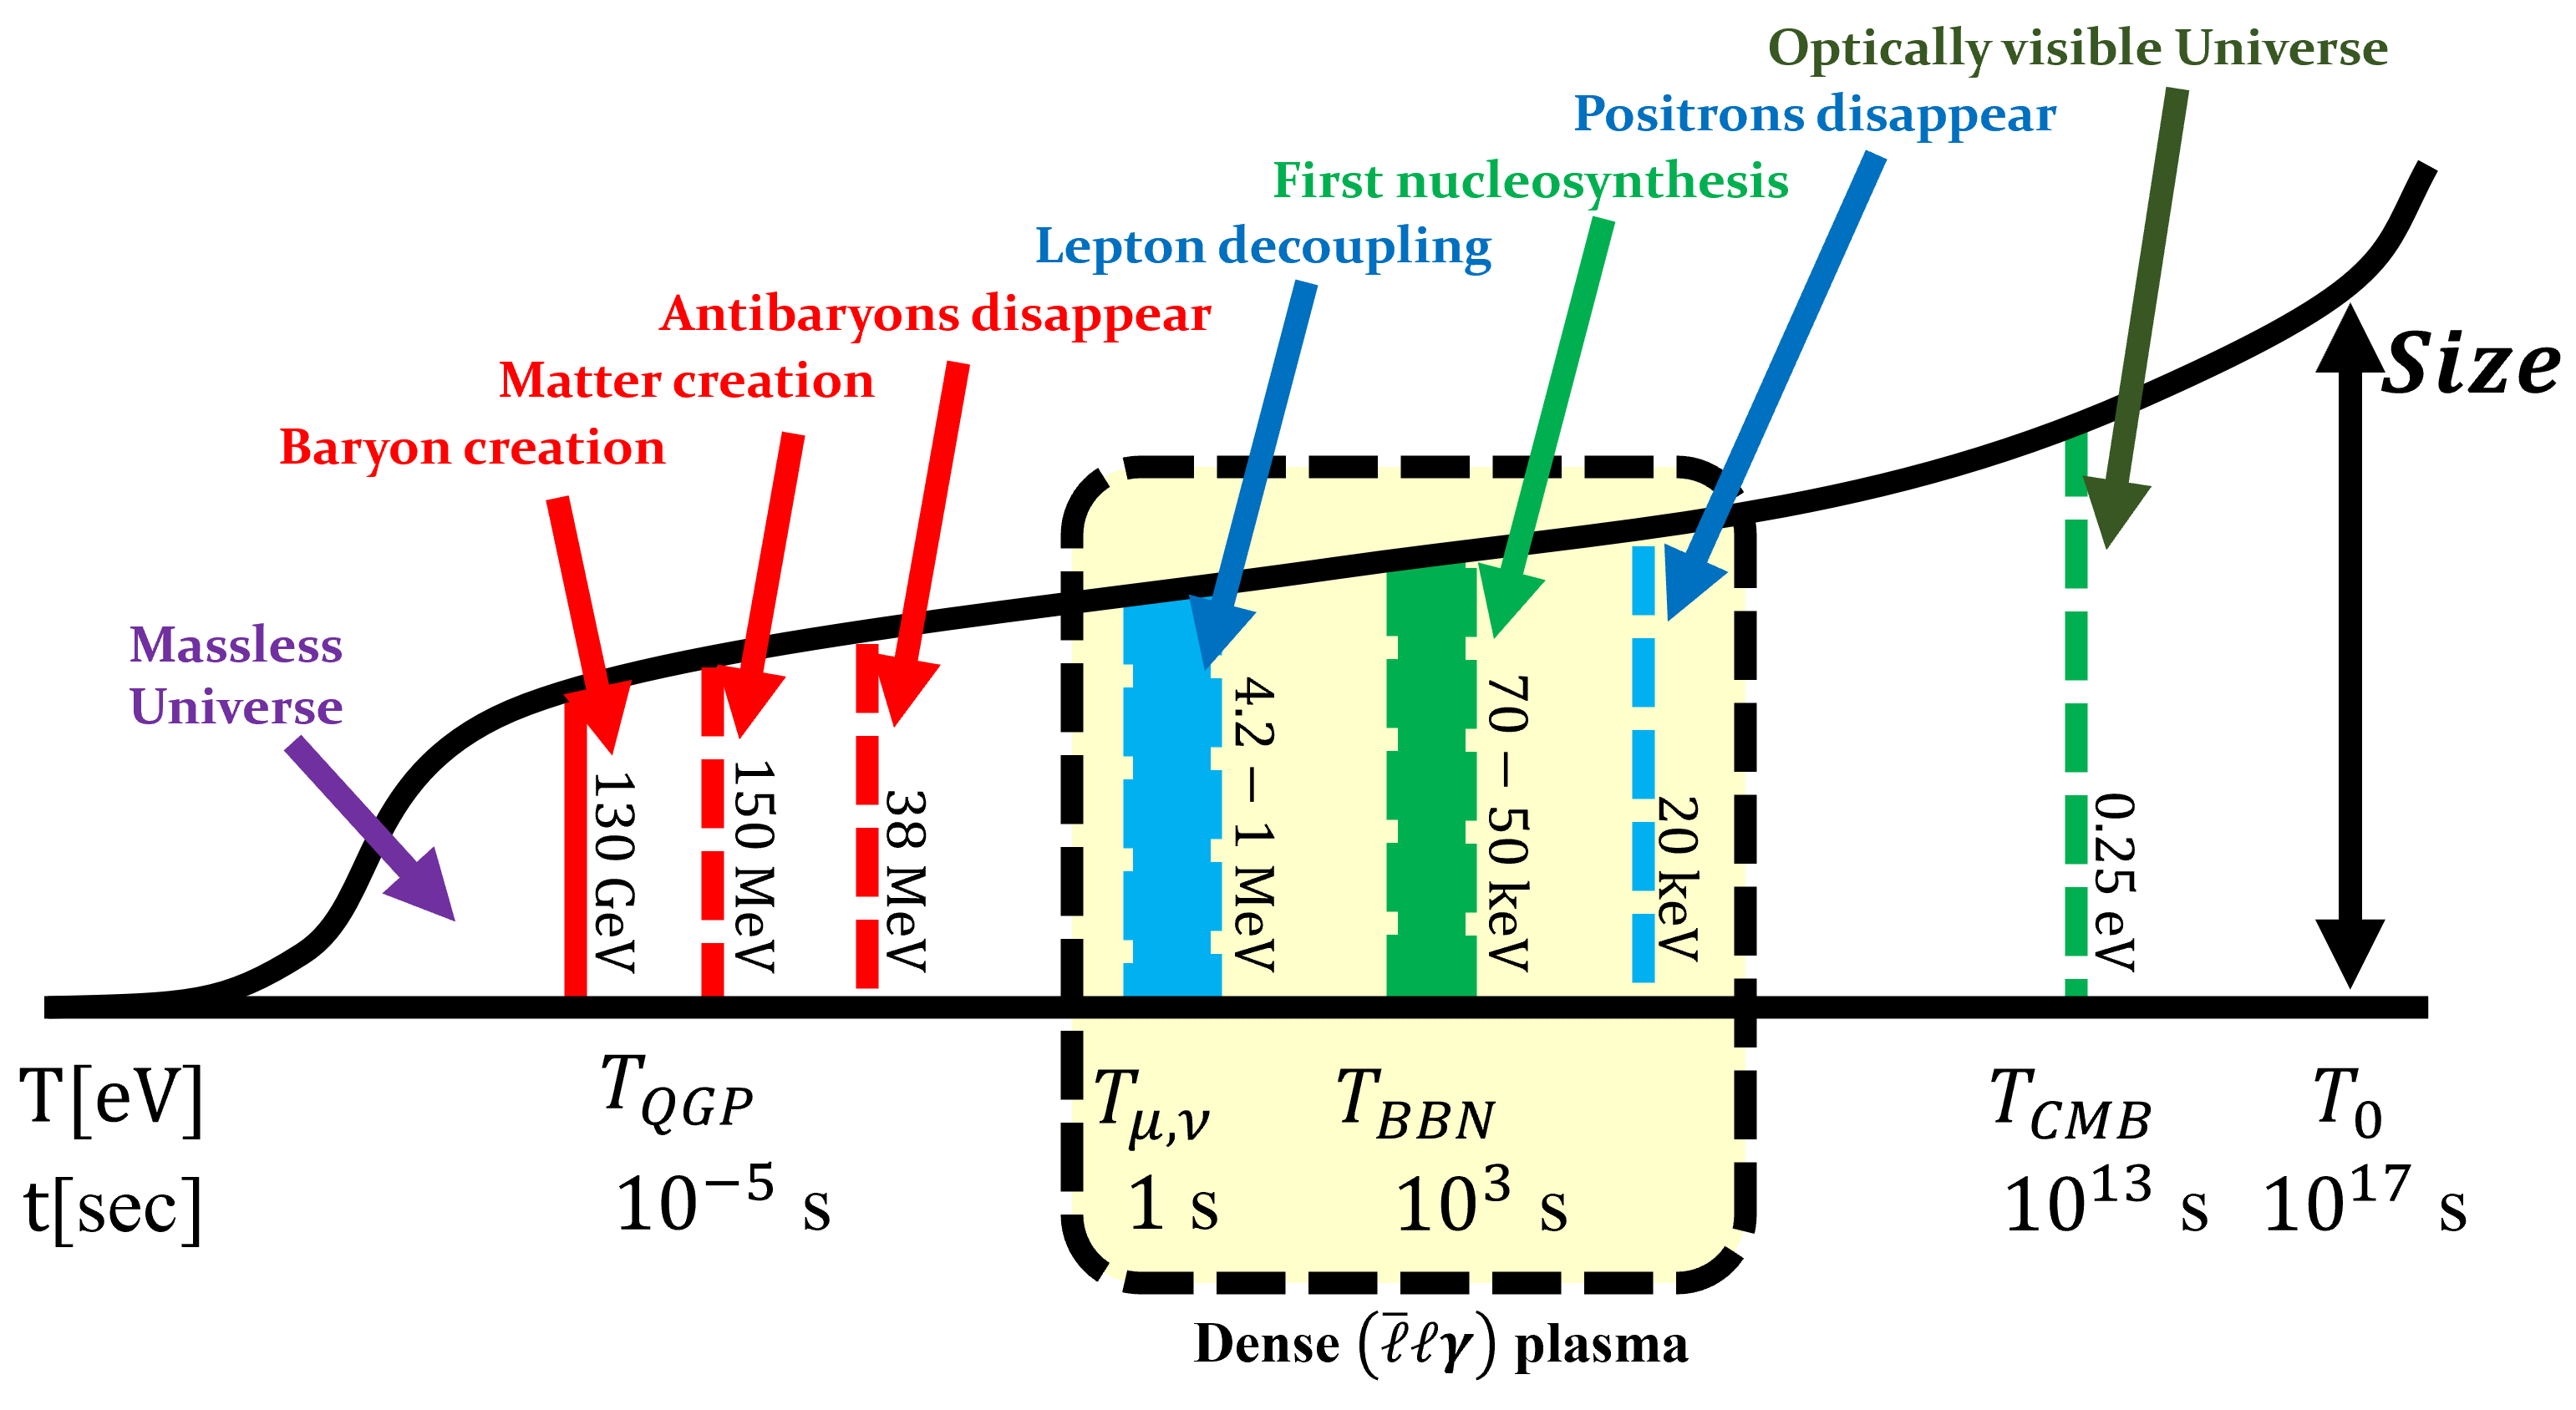
\includegraphics[width=0.95\linewidth]{plots/chap01intro/thesis_universe.png}
 \caption{A schematic of the universe's evolution since the Big Bang. The region of interest studied in this dissertation is emphasized (in the highlighted box) to contain a dense nearly charge neutral matter-antimatter plasma.}
 \label{fig:cosmo} 
\end{figure}
%%%%%%%%%%%%%%%%%%%%%%%%%%%%%%%%%%%%%%%

The scale factor $a(t)$ denotes the change of proper distances $L(t)$ over time as
\begin{gather}
    L(t)=L_{0}\frac{a_{0}}{a(t)}\rightarrow L(z)=L_{0}(1+z)\,,
\end{gather}
where $z$ is the redshift and $L_{0}$ the comoving length. In an expanding (or contracting) universe which is both homogeneous and isotropic. This implies volumes change with $V(t)=V_{0}/a^{3}(t)$ where $V_{0}=L_{0}^{3}$ is the comoving Cartesian volume. The evolutionary expansion of the universe is then traditionally defined in terms of the Hubble parameter $H(t)$ following the conventions in~\cite{weinberg1972gravitation}
\begin{gather}
  \label{Friedmann:1} H(t)^{2}\equiv\left(\frac{\dot a}{a}\right)^2=\frac{8\pi G_{N}}{3}\rho_\mathrm{total},\qquad \rho_\mathrm{total}(t)=\rho_{\Lambda}+\rho_\mathrm{DM}(t)+\rho_\mathrm{Baryons}(t)+\ldots\\
  \label{Friedmann:2}
  \frac{\ddot a}{a}=-qH^2,\qquad 
q\equiv -\frac{a\ddot a}{\dot a^2},\qquad \dot H=-H^2(1+q).
\end{gather}
where $G_N$ is the Newtonian constant of gravitation. \req{Friedmann:1} and \req{Friedmann:2} are also known as the Friedmann equations. The total density $\rho_\mathrm{total}$ is the sum of all contributions from any form of matter, radiation or field. This includes but is not limited to: dark energy $(\Lambda)$, dark matter (DM), baryons (B), leptons $(\ell,\nu)$ and photons $(\gamma)$. Depending on the age of the universe, the relative importance of each group changes as each dilutes differently under expansion with dark energy infamously remaining constant in density and accelerating the universe today.

The parameter $q$ is the cosmic deceleration which for historical reasons is positive $q>0$ under deceleration. This convention was chosen before the discovery of dark energy under the tacit assumption that the universe would be decelerating. The value of $q$ depends on energy content: The early universe was radiation dominated $(q = 1)$, subsequently matter dominated $(q = 1/2)$, and lastly the contemporary universe is undergoing a transition from matter to dark energy dominated approaching the asymptotic value of $q = -1$; see~\cite{Rafelski:2013yka}.

We can consider the expansion to be an adiabatic process~\cite{Abdalla:2022yfr} which results in a smooth shifting of the relevant dynamical quantities. As the universe undergoes isotropic expansion, the temperature decreases as 
\begin{gather}
 \label{tscale}
 T(t)=T_{0}\frac{a_{0}}{a(t)}\rightarrow T(z)=T_{0}(1+z)\,,
\end{gather}
where $z$ is the redshift. The entropy within a comoving volume is kept constant until gravitational collapse effects become relevant. The comoving temperature $T_{0}$ is given by the the present CMB temperature $T_{0}=2.7{\rm\ K}\simeq2.3\times10^{-4}\eV$~\cite{Planck:2018vyg}, with contemporary scale factor $a_{0}=1$.

As the universe expands, redshift reduces the momenta of particles lowering their contribution to the energy content of the universe. This cosmic redshift is written as
\begin{alignat}{1}
  \label{Redshift} p_{i}(t) = p_{i,0}\frac{a_{0}}{a(t)}\,.
\end{alignat}
Momentum (and the energy of massless particles $E=pc$) scales with the same factor as temperature. The energy of massive free particles in the universe however scales differently based on their momentum (and thus temperature).

When hot and relativistic, particle energy decreases inversely with scale factor like radiation. As the particles transition to non-relativistic (NR) energies, they decrease with the inverse square of the scale factor
\begin{alignat}{1}
    \label{EScale} E(t) = E_{0}\frac{a_{0}}{a(t)}\xrightarrow{\mathrm{NR}}\  E_{0}\frac{a_{0}^{2}}{a(t)^{2}}\,.
\end{alignat}
This occurs because of the functional dependence of energy on momentum in the relativistic $E\sim p$ versus non-relativistic $E\sim p^{2}$ cases.

\subsection{The standard FLRW-Universe model}
%In this section we will focus on the following:
%\begin{itemize}
%    \item The Robertson –Walker Universe
%    \item The Friedmann equation (Hubble %    \item The composition of the universe
%\end{itemize}
The Friedmann-Lemaitre-Robertson-Walker (FLRW) Universe is a theoretical model used widely to describe the cosmological evolution of the Universe. It is based on the cosmological principles which assumes homogeneity and isotropy of the Universe on large scales. In general, the FLRW metric can be written as
\begin{align}\label{metric}
ds^2=c^2dt^2-a^2(t)\left[ \frac{dr^2}{1-kr^2}+r^2(d\theta^2+\sin^2\theta\,d\phi^2)\right].
\end{align}
The metric is characterized by the scale factor $a(t)$ which measures the size of the Universe as a function of time $t$. The geometric parameter $k$ identifies the Gaussian geometry of the spatial hyper-surfaces defined by co-moving observers. The metrics are qualitatively different depending on the value of $k$. We have $k=1$ which correspond to the closed Universe,  $k=0$ correspond to flat Universe, and $k=-1$ for open geometries of the Universe. Current observation of cosmic microwave background (CMB) anisotropy preferred value $k=0$~[\cite{Planck:2013pxb,Planck:2015fie,Planck:2018vyg}].


The cosmological equations that describe the evolution of the Universe are derived from the Einstein equations. In general, the Einstein equation with cosmological constant $\Lambda$ can be written as:
\begin{equation}\label{Einstein}
  G^{\mu\nu}=R^{\mu\nu}-\left(\frac R 2 +\Lambda\right) g^{\mu\nu}=8\pi G_N T^{\mu\nu}, 
\quad R= g_{\mu\nu}R^{\mu\nu}.  
\end{equation}
where $G_{N}$ is the Newtonian gravitational constant, and $T^{\mu\nu}$ is the stress-energy tensor. Given the homogeneous and isotropic symmetry conditions imply that the matter context of the Universe can be expressed as a perfect fluid. The stress-energy tensor $T^\mu_\nu$ of perfect fluid can be written as
\begin{align}
 T^\mu_\nu =\mathrm{diag}(\rho, -P, -P, -P).
\end{align}
where $\rho$ is energy density and an $P$ is the isotropic pressure.

Substituting the perfect fluid form of the stress-energy tensor into the Einstein equations, one can derive the cosmological equations that describe the evolution of the Universe. We then obtain Friedmann equations as follows:
\begin{align}
\label{Hubble} 
&H^{2}\equiv\left(\frac{\dot a}{a}\right)^2=\frac{8\pi G_{N}}{3}\rho-\frac{k}{a^2}+\frac{\Lambda}{3},\\
\label{q_value}
&qH^2=\frac{4\pi G_{N}}{3}\left(\rho+3P\right)-\frac{\Lambda}{3},\qquad q\equiv -\frac{a\ddot a}{\dot a^2},
\end{align}
where $H$ is the Hubble parameter,  $q$ is the deceleration parameter. These equations relate the dynamics of the scale factor $a(t)$ to the energy density and pressure of the cosmic plasma. On the other hand, considering the divergence freedom of the total stress-energy tensor $\nabla_\nu T^{\mu\nu}=0$. For $\mu=0$ component, we have
\begin{align}\label{energy_eq}
\nabla_\nu T^{0\nu}=\frac{d\rho}{dt}+3H(\rho+P)=0
\end{align}
which provides dynamical evolution equation for $\rho(t)$ and $P(t)$. Solutions of Eq.~(\ref{energy_eq}) describes the time evolution of  energy density and pressures in the Universe. Given the energy density and pressure as a function of time, we can illustrates how the Universe evolves according to the Friedmann equations Eq.~(\ref{Hubble}) and Eq.~(\ref{q_value}). Solving these equations allows us to understand the dynamics and evolution of the Universe such as the Hubble expansion and the behavior of matter and energy over cosmic time.

\subsection{Cosmic plasma in early Universe $300\,\mathrm{MeV}>T>0.02\,\mathrm{MeV}$}
%In this section we will focus on the following:
%\begin{itemize}
%    \item Five different plasma epoch from $0.3\mathrm{GeV}>T>20$keV
%\end{itemize}

The primordial hot Universe fireball underwent several practically adiabatic phase changes that dramatically evolved its bulk properties as it expanded and cooled~[\cite{Rafelski:2023emw}]. We present an overview of the Universe evolution as a function of temperature from $300\,\mathrm{MeV}>T>0.02\,\mathrm{MeV}$ and main events constituting the history of the early Universe in Fig.~\ref{Overview_fig}. After the electroweak symmetry breaking epoch and presumably inflation, the comic plasma in the early Universe evolves in the following sequence:

%%%%%%%%%%%%%%%%%%%%%%%%%%%%%%%%%%%%%%%
\begin{figure}[ht]
 \centerline{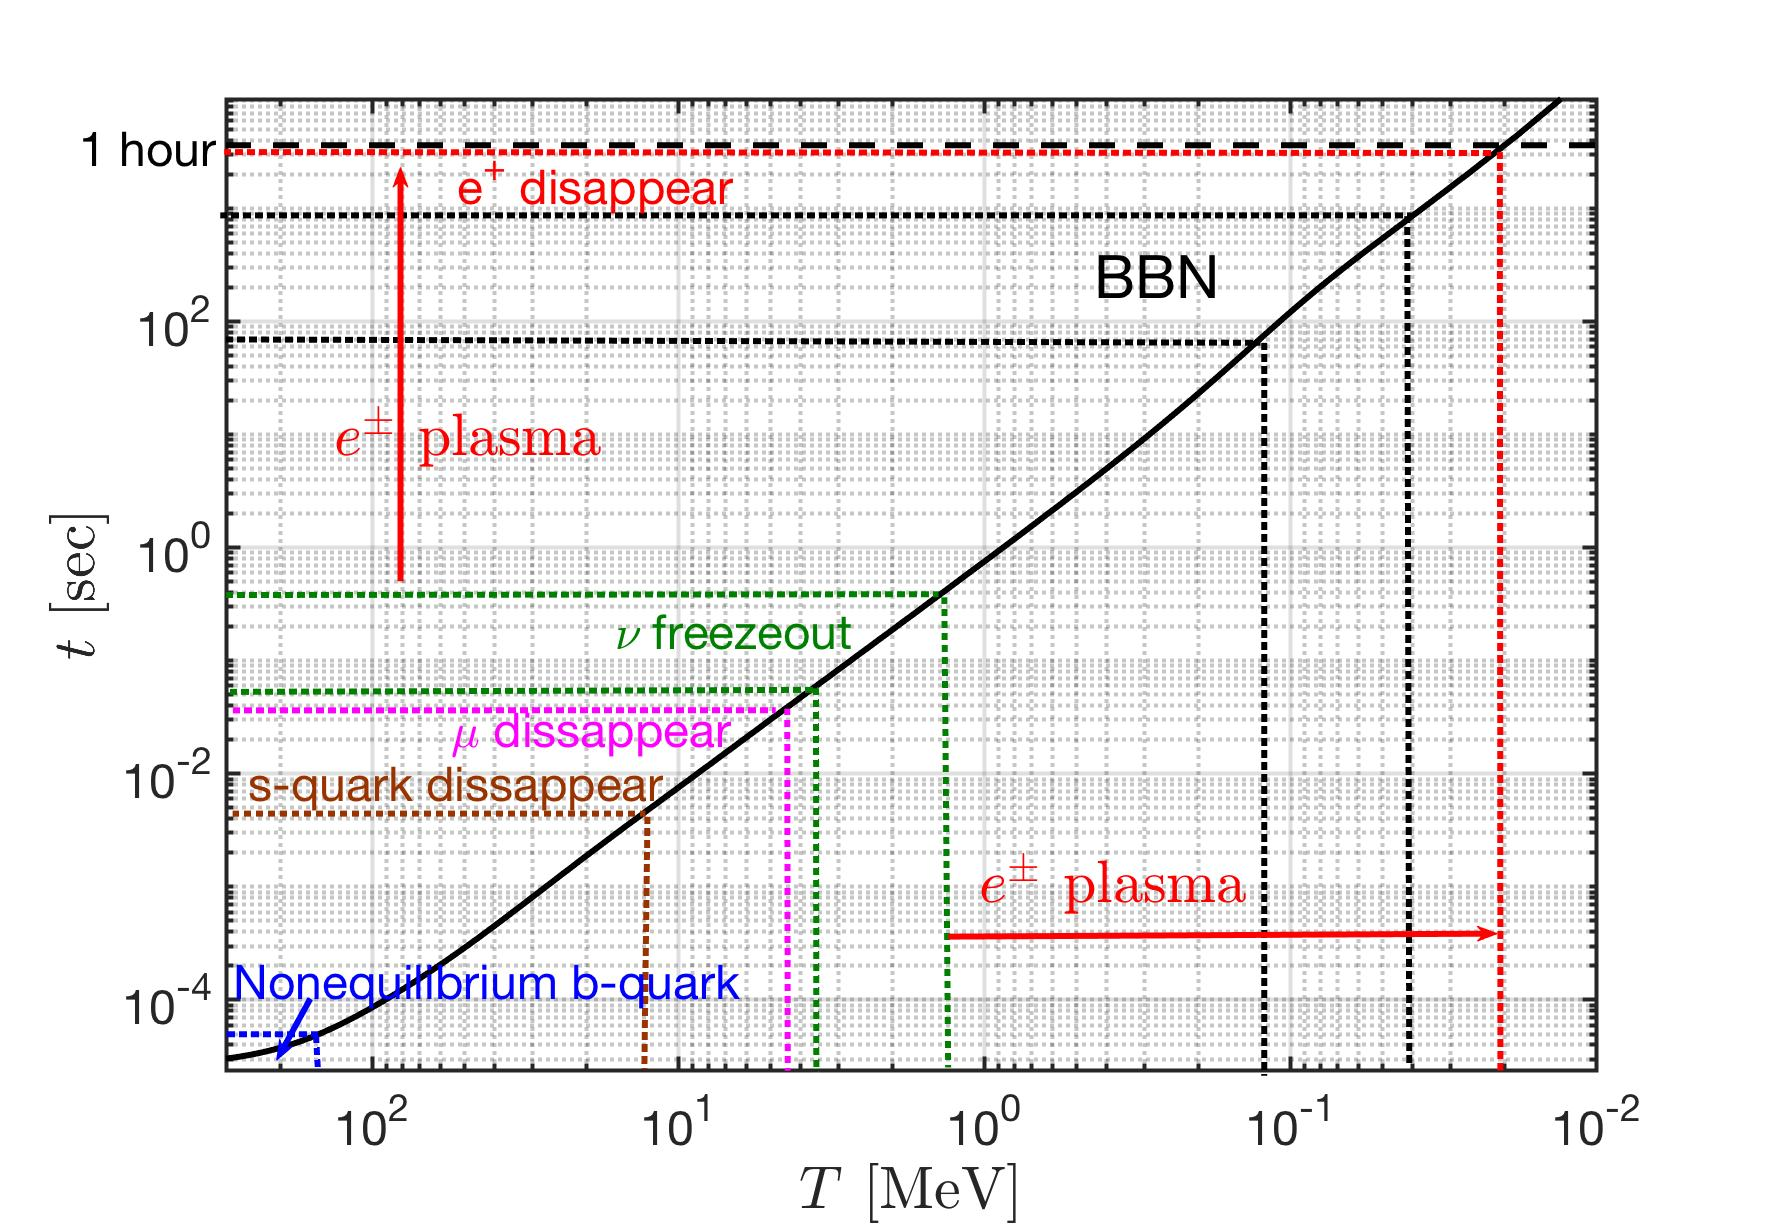
\includegraphics[width=\textwidth,width=\linewidth]{./plots/CosmicTimeTemperature_Project}}
 \caption{The time evolution of the early Universe as a function of temperature from $300\,\mathrm{MeV}>T>0.02\,\mathrm{MeV}$ and 
 different sequence of main events are shown with the temperature/time range in the evolution. }
 \label{Overview_fig}
\end{figure}
%%%%%%%%%%%%%%%%%%%%%%%%%%%%%%%%%%%%%%%

\begin{enumerate}
    \item \textbf{Primordial quark-gluon plasma}: 
    At early times when the temperature was between $130\,\mathrm{GeV}>T>0.15\,\mathrm{GeV}$ we have the building blocks of the Universe as we know them today, including the leptons, vector bosons, and all three families of deconfined quarks and gluons which propagated freely in plasma. As all hadrons are dissolved into their constituents during this time, strongly interacting particles $u,d,s,t,b,c,g$ controlled the fate of the Universe. When temperature is near to the QGP phase transition $300\, \mathrm{MeV}>T>150$ MeV, the bottom quark  breaks the detail balance and disappearance from particle inventory provides the arrow in time (see Chapter~\ref{Bottom} for detail).
    
    \item \textbf{Hadronic epoch}: Around the hadronization temperature $T_H\approx150\,\mathrm{MeV}$, a phase transformation occurred, forcing 
    the free quarks and gluons become confined within baryon and mesons [\cite{Letessier:2005qe}]. In the temperature range $ 150\,\mathrm{MeV}>T>20\,\mathrm{MeV}$, the Universe is rich in physics phenomena involving strange mesons and (anti)baryons including (anti)hyperon abundances~[\cite{Fromerth:2012fe,Yang:2021bko}]. The antibaryons disappear from the Universe at temperature $T=38.2$ MeV, and strangeness can be produced by the inverse decay reactions that are in equilibrium via weak, electromagnetic, and strong interactions in the early Universe until $T\approx13$ MeV (see Chapter~\ref{Strangeness} for detailed discussion).

    
    \item \textbf{Lepton-photon epoch}: For temperature $10\,\mathrm{MeV}>T>2\,\mathrm{MeV}$, the Universe contained relativistic electrons, positrons, photons, and three species of (anti)neutrinos. During this epoch massless leptons and photons controlled the fate of the Universe. Massive $\tau^\pm$ disappear from the plasma at high temperature via decay processes. However $\mu^\pm$ leptons can persist in the early Universe until temperature $T=4.2$ MeV, and positron $e^+$ can persist until the temperature $T=0.02$ MeV (See Chapter~\ref{Electron} for discussion).
    Neutrinos were still coupled to the charged leptons via the weak interaction~[\cite{Birrell:2012gg,Birrell:2014ona}] and freeze-out at temperature range $3\,\mathrm{MeV}>T>2\,\mathrm{MeV}$ which depends on the neutrino's flavors and the magnitude of the Standard Model parameters (See Chapter~\ref{Neutrino} for details). After neutrino freeze-out, they still play a important role in the Universe expansion via the effective number of neutrinos $N_{\nu}^{\mathrm{eff}}$ and affects the Hubble parameter significantly.  
    
    \item \textbf{Electron-positron epoch}: After neutrinos freeze-out at $T=3\sim2\,\mathrm{MeV}$ and become free-streaming in the early Universe, the cosmic plasma was dominated by electrons, positrons, and photons. The $e^\pm$ plasma existed until $T\approx0.02\,\mathrm{MeV}$ such that BBN occurred within a rich electron-positron plasma, and the dense number density of electron/positron also provide the opportunities to investigate magnetization process (See Chapter~\ref{Electron} for detailed discussion). This is the last time the Universe will contain a significant fraction of its content in antimatter.
\end{enumerate}
After $e^\pm$ annihilation, the Universe was still opaque to photons at this point and remained so until the recombination period at $T\approx0.25\,\mathrm{eV}$ starting the era of observational cosmology with the Cosmic Microwave Background. This period has been studied in detail before in~[\cite{Planck:2018vyg}]. Therefore, we focus on the temperature $300\,\mathrm{MeV}>T>0.02\,\mathrm{MeV}$ which corresponds to the first hour of the Universe evolution. We will address the cosmic plasma as follow: In Chapter~\ref{Bottom}, we discuss the heavy quarks (bottom/charm) abundance near to the QGP hadronization and show the nonequilibrium of bottom quark.  In Chapter~\ref{Strangeness} we study the strangeness abundance after hadronization and show the long lasting strangeness in the early Universe. In Chapter~\ref{Neutrino} we focus on the neutrino-matter interactions and the evolution of cosmic neutrino in early universe before/after freeze-out. In Chapter~\ref{Electron} we study the abundance of charged leptons $\mu^\pm$ and $e^\pm$ and show that the present of $e^\pm$ plasma plays an important role in early Universe. In Chapter~\ref{Outlook} we address the ongoing and prospective research projects for future publication.
Finally in Chapter~\ref{Summary} we summarize the important results of our study and conclusion.

\section{Introduction to Cosmology and the Relic Neutrino Background}\label{ch:intro}
At a temperature of $5$ MeV the Universe consisted of a plasma of $e^\pm$, photons, and neutrinos. At around $1$ MeV neutrinos stop interacting, or freeze-out, and begin to free-stream through the Universe. Today they comprise the relic neutrino background. Photons freeze-out around $0.25$ eV and today they make up the Cosmic Microwave Background (CMB), currently at $T_{\gamma,0}=0.235$ meV.  Relic neutrinos have not been directly measured, but their impact on the speed of expansion of the Universe is imprinted on the CMB.  Indirect measurements of the relic neutrino background, such as by the Planck satellite \cite{Planck},  constrain neutrino properties such as mass and number of massless degrees of freedom.

 In later chapters, we will study the details of the neutrino freeze-out process and their impact on observables in detail but first we present an overview of cosmology, from just prior to neutrino freeze-out until today, putting the relic neutrinos in their proper context. Much of this material, including most figures, was adapted from our paper \cite{ErasOfUniverse}.


\subsection{Standard Cosmology}\label{cosmo}
 To follow the history of the relic neutrino distribution, one must first understand the relation between the expansion dynamics of the Universe, its energy content, and the connection to the photon and neutrino temperature. For this purpose we need some preparation in the  Friedmann$-$Lemaitre$-$Robertson$-$Walker (FRW) cosmological  model, see for example \cite{hartle2003gravity,hobson,misner1973gravitation}. Assuming a homogeneous, isotropic Universe, one arrives at the spacetime metric
\beqn\label{metric}
ds^2=dt^2-a^2(t)\left[ \frac{dr^2}{1-kr^2}+r^2(d\theta^2+\sin^2(\theta)d\phi^2)\right]
%g_{00}=1, \quad g_{rr}=-\frac{a^2}{1-kr^2}, \quad g_{\theta\theta}=-a^2r^2, \quad g_{\phi\phi}=-a^2 r^2\sin^2\theta
\eeqn
characterized  by the scale parameter $a(t)$.  $a(t)$ determines the distance between objects at rest in the Universe frame, otherwise known as comoving observers. The geometric parameter $k=-1,0,1$ identifies the geometry of the spacial hypersurfaces defined by comoving observers. Space is a flat-sheet for the observationally preferred value $k=0$ \cite{Planck}, hyperbolic for $k=-1$, and spherical for $k=1$.

The dynamics are governed by the Einstein equations
\beqn\label{Einstine}
G^{\mu\nu}=R^{\mu\nu}-\left(\frac R 2 -\Lambda\right) g^{\mu\nu}=-\frac{1}{M_p^2} T^{\mu\nu},  
\quad R= g_{\mu\nu}R^{\mu\nu}
\eeqn
where $M_p\equiv 1/\sqrt{8\pi G_N}$ is the Planck mass, $G_N$ is the gravitational constant, and we work in units where $\hbar=c=1$. Recall that the Einstein tensor $G^{\mu\nu}$ is divergence free and hence so is the total stress energy tensor, $T^{\mu\nu}$.  Note that our definition of $M_p$, while more convenient in cosmology, differs by a factor of $1/\sqrt{8\pi}$ from the particle physics convention.  Finally, we point out that there are several sign conventions in use regarding the definition of geometrical quantities and Einstein's equation that are clarified in appendix \ref{app:conventions}.

 In a homogeneous isotropic spacetime, the matter content is necessarily characterized by two quantities, the energy density $\rho$ and isotropic pressure $P$
\begin{equation}
  T^\mu_\nu =\mathrm{diag}(\rho, -P, -P, -P).
\end{equation}
 It is common to absorb the Einstein cosmological constant $\Lambda$ into $\rho$ and $P$ by defining
\beqn\label{EpsLam}
\rho_\Lambda=M_p^2\Lambda, \qquad P_\Lambda=-M_p^2 \Lambda.
\eeqn
We implicitly consider this done from now on. 


The global Universe dynamics can be characterized by two  quantities, the Hubble parameter  $H$, a strongly time dependent quantity on cosmological time scales,  and the deceleration parameter $q$
\beqn\label{dynamic}
\frac{\dot a }{a}\equiv H(t) ,\quad 
q\equiv -\frac{a\ddot a}{\dot a^2}.
\eeqn
We note the relations
\beqn
\quad \frac{\ddot a}{a}=-qH^2,\quad \dot H=-H^2(1+q). 
\eeqn

Two dynamically independent equations arise using the metric \req{metric} in \req{Einstine}
\beqn\label{hubble}
\frac{8\pi G_N}{3} \rho =  \frac{\dot a^2+k}{a^2}
=H^2\left( 1+\frac { k }{\dot a^2}\right),
\qquad
\frac{4\pi G_N}{3} (\rho+3P)  =-\frac{\ddot a}{a}=qH^2.
\eeqn
We can eliminate the strength of the interaction, $G_N$,  solving both these equations for ${8\pi G_N}/{3}$, and equating the result to find a relatively simple constraint for the deceleration parameter
\beqn\label{qparam}
q=\frac 1 2 \left(1+3\frac{P}{\rho}\right)\left(1+\frac{k}{\dot a^2}\right).
\eeqn
 From this point on, we work within the  flat cosmological model with $k=0$ and so $q$ is determined entirely by the matter content of the Universe
\begin{equation}\label{qparam}
q=\frac 1 2 \left(1+3\frac{P}{\rho}\right).
\end{equation}


As must be the case for any solution of Einstein's equations,   \req{hubble} implies that the energy momentum tensor of matter is divergence free
\beqn\label{divTmn}
\nabla_\nu T^{\mu\nu} =0 \Rightarrow -\frac{\dot\rho}{\rho+P}=3\frac{\dot a}{a}=3H.
\eeqn
 The same relation also follows from  conservation of entropy, $dE+PdV=TdS=0,\  dE=d(\rho V),\  dV=d(a^3)$. Given an equation of state $P(\rho)$, solution of \req{divTmn} describes the dynamical evolution of matter in the Universe. Combined with the Hubble equation
\begin{equation}\label{Hubble_eq}
H^2=\frac{\rho}{3M_p}
\end{equation}
this allows us to solve for the large scale dynamics of the Universe. 

Using the flat FRW model of cosmology outlined above, we now present several perspectives on the history of the Universe.  First we focus on the reheating history. 

%%%%%%%%%%%%%%%%%%%%%%%%%%%%%%%%%%%%%%%%%%%%%%%%%%%%%%%%%%%%%%%
\subsection{Reheating History of the Universe}\label{Eralink}

At times where dimensional scales are irrelevant, entropy conservation means that  temperature scales inversely with the scale factor $a(t)$. This follows from \req{divTmn} when $ \rho\simeq 3P   \propto T^4$. However, as the temperature drops and at their respective $m\simeq T$ scales, successively less massive particles annihilate and disappear from the thermal Universe. Their entropy reheats the other degrees of freedom and thus in the process, the entropy originating in a massive degree of freedom is shifted into the effectively massless degrees of freedom that still remain.  This causes the  $T\propto 1/a(t)$ scaling to break down; during each of these `reorganization' periods the drop in temperature is slowed by the concentration of entropy in fewer degrees of freedom, leading to a change in the reheating ratio, $R$, defined as
\begin{equation}\label{redshiftratio}
R\equiv \frac{1+z}{ T_\gamma/T_{\gamma,0}}, \qquad 1+z\equiv \frac{a_{0}}{a(t)}.
\end{equation}
The reheating ratio connects the photon temperature redshift to the geometric redshift, where $a_0$ is the scale factor today (often normalized to $1$) and quantifies the deviation from the scaling relation between $a(t)$ and $T$.

As we will see, the change in $R$ can be computed by the drop in the number of degrees of freedom.  At a temperature on the order of the top quark mass, when all standard model particles were in thermal equilibrium, the Universe was pushed apart by 28 bosonic and 90 fermionic degrees of freedom. The total number of degrees of freedom can be computed as follows.  

For bosons we have the following: the doublet of charged Higgs particles has $4=2\times2=1+3$  degrees of freedom -- three will migrate to the longitudinal components of $W^\pm, Z$ when the electro-weak vacuum freezes and the EW symmetry breaking arises, while one is retained in the one single dynamical charge neutral Higgs component. In the massless stage, the SU(2)$\times$U(1) theory has 4$\times$2=8 gauge degrees of freedom where the first coefficient  is  the number of particles $(\gamma, Z, W^\pm)$ and each massless gauge boson has  two transverse polarizations. Adding in $8_c\times2_s=16$ gluonic degrees of freedom we obtain 4+8+16=28  bosonic degrees of freedom. 

The count of fermionic degrees of freedom includes three $f$ families, two spins $s$, another factor two for particle-antiparticle duality. We have in each family of flavors a doublet of $2\times 3_c$ quarks, 1-lepton and 1/2 neutrinos (due left-handedness which was not implemented counting spin). Thus we find that a total $3_f\times 2_p\times 2_s\times(2\times 3_c+1_l+1/2_\nu)=90$ fermionic degrees of freedom. We further recall that massless fermions contribute 7/8 of that of bosons in both pressure and energy density. Thus the total number of massless Standard Model particles at a temperature above the top quark mass scale, referring by convention to bosonic degrees of freedom, is $g_{\rm SM}=28+90\times 7/8=106.75$ 



In figure~\ref{fig:dof}  we show the cube of the reheating ratio \req{redshiftratio} as a function of photon temperature $T_\gamma$ from the primordial high temperature  early Universe on the right to the present on the left, where $R$  must be by definition unity.  The periods of change seen in figure \ref{fig:dof} come when the temperature crosses the mass of a particle species that is in equilibrium. One can see drops corresponding to the disappearance of particles as indicated.   After $e^+e^-$ annihilation on the left, there are no significant degrees of freedom remaining to annihilate and feed entropy into photons, and so $R$  remains constant until today. We show the result using a Fermi gas model with a very rough model for the QGP phase transition and hadronization period near $O(100\MeV)$. The fermi gas model is a poor approximation above the QGP phase transition; a more precise model using lattice QCD, see e.g. \cite{Borsanyi:2013bia}, together with a high temperature perturbative QCD expansion, see e.g. \cite{letessier2002hadrons}, would be needed to improve on this situation but the details do not impact the neutrino freeze-out period near $1\MeV$ which is our primary concern, and so we do not consider these issues further here.

%%%%%%%%%%%%%%%%%%%%%%%%%%%%%%%%%%%%%%%
\begin{figure} 
\centerline{\hspace*{0.4cm}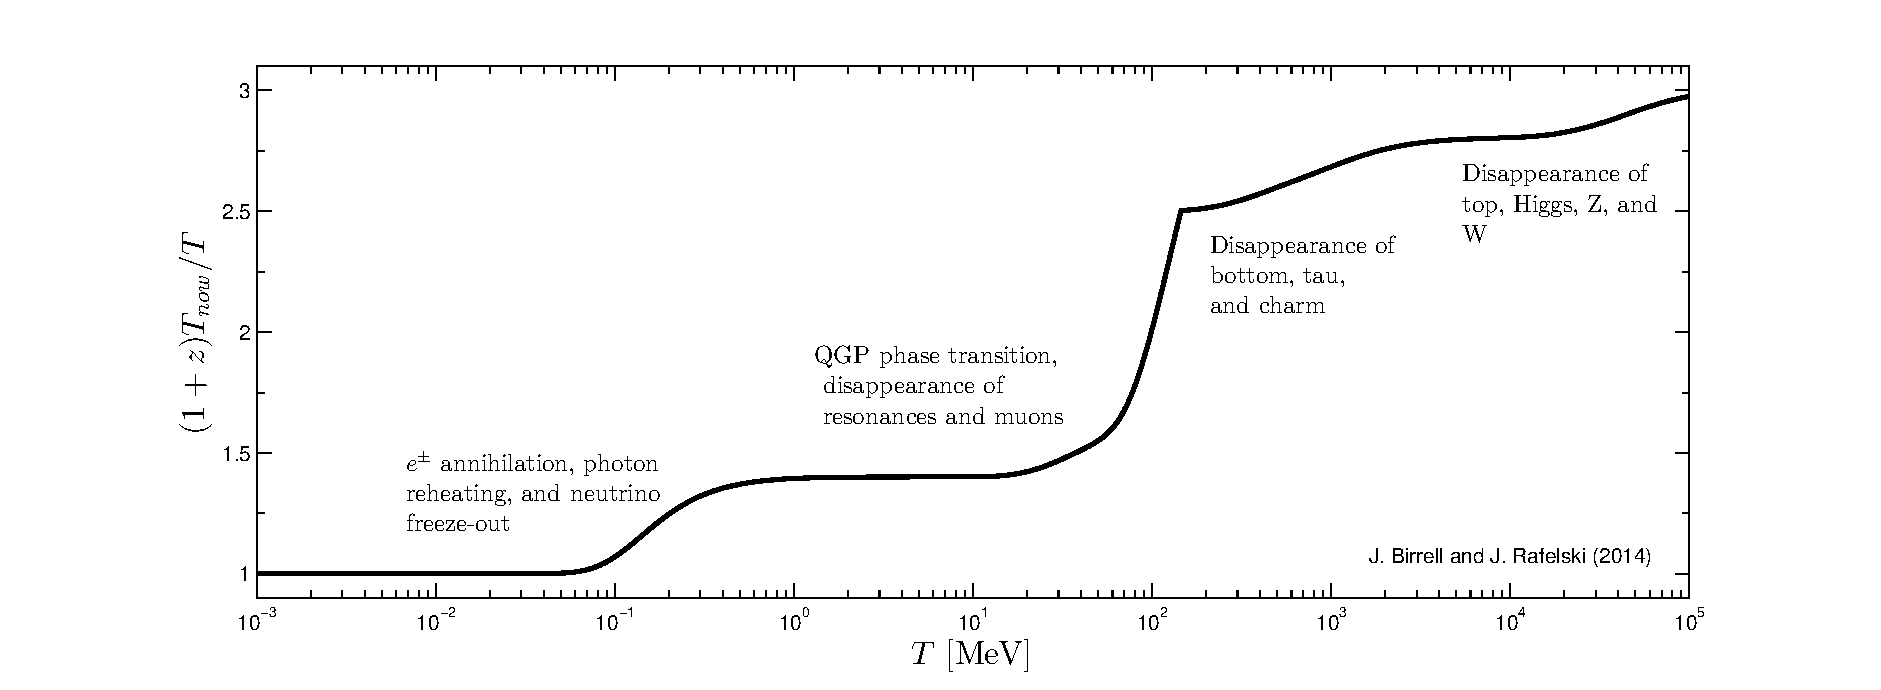
\includegraphics[height=6.6cm]{03-birrell/ErasOfUniverse/z_T_plot.eps}}
\caption{Disappearance of degrees of freedom. The Universe volume inflated approximately by a factor of 27 above the thermal red shift scale as massive particles disappeared successively from the inventory.\label{fig:dof}}
 \end{figure}
%%%%%%%%%%%%%%%%%%%%%%%%%%%%%%%%%%%%%%%



As long as the dynamics are at least approximately entropy conserving, the total drop in $R$ is entirely determined by entropy conservation. Namely, the magnitude of the drop in $R$ figure~\ref{fig:dof} is a measure of the number of degrees of freedom that have disappeared from the Universe. Consider   two times $t_1$ and $t_2$ at which all particle species that have not yet annihilated are effectively massless.  By conservation of comoving entropy and  scaling $T\propto 1/a$ we have
\begin{equation}\label{r_ratio}
1=\frac{a_1^3S_{1}}{a_2^3 S_2}=\frac{a_1^3\sum_ig_i T_{i,1}^3}{a_2^3\sum_j g_j T_{j,2}^3},\qquad \left(\frac{R_1}{R_2}\right)^3=\frac{\sum_ig_i (T_{i,1}/T_{\gamma,1})^3}{\sum_j g_j (T_{j,2}/T_{\gamma,2})^3}
\end{equation}
where the sums are over the total number of degrees of freedom present at the indicated time and the degeneracy factors $g_i$ contain the $7/8$ factor for fermions. In the second form    we divided the numerator and denominator by $a_{0}T_{\gamma,0}$. We distinguish between the temperature of each particle species and our reference temperature, the photon temperature.  This is important since today neutrinos are colder than photons, due to photon reheating from  $e^\pm$ annihilation occurring after neutrinos decoupled (this is only an approximation, a point we will study in detail in subsequent chapters).  By conservation of entropy one obtains the neutrino to photon temperature ratio of
\begin{equation}\label{T_nu_T_gamma}
T_\nu/T_\gamma=({4}/{11})^{1/3}.
\end{equation}
We will call this the reheating ratio in the decoupled limit.  For details on the derivation of this standard result, see for example our paper in appendix \ref{app:model_ind}, where it is obtained as a special case of a more general analysis. 

Using \req{r_ratio}  we  compute the total drop in $R^3$ shown in figure \ref{fig:dof}.  At $T=T_\gamma=\mathcal{O}(100\GeV)$ the number of active degrees of freedom is slightly below $g_{\rm SM}=106.75$ due to the partial disappearance of top quarks, but this approximation will be good enough for our purposes.  At this time, all the species are in thermal equilibrium with photons and so $T_{i,1}/T_{\gamma,1}=1$ for all $i$.  Today we have $2$ photon and $7/8\times 6$ neutrino degrees of freedom and a  neutrino to photon temperature ratio \req{T_nu_T_gamma}.  Therefore we have
\begin{equation}
\left(\frac{R_{100GeV}}{R_{now}}\right)^3= \frac{g_{SM}}{g_{\rm now}}=\frac{106.75}{2+\frac{7}{8}\times 6\times \frac{4}{11}}\approx 27.3
\end{equation}
which is the  fractional change we see in the fermi gas model curve in figure \ref{fig:dof} (as mentioned above, the QCD model is reduced due to interactions). The meaning of this factor is that the Universe approximately inflated by a factor 27 above the thermal red shift scale as massive particles disappeared successively from the inventory. 


\subsection{Composition of the Universe}
From the perspective of reheating, the history of the Universe from the end of $e^\pm$ annihilation until today has been uneventful.  We can shed additional light on this period and others by looking at the composition of the Universe as a function of temperature

%%%%%%%%%%%%%%%%%%%%%%%%%%%%%%%%%%%%
\begin{figure}
\centerline{\hspace*{0.4cm}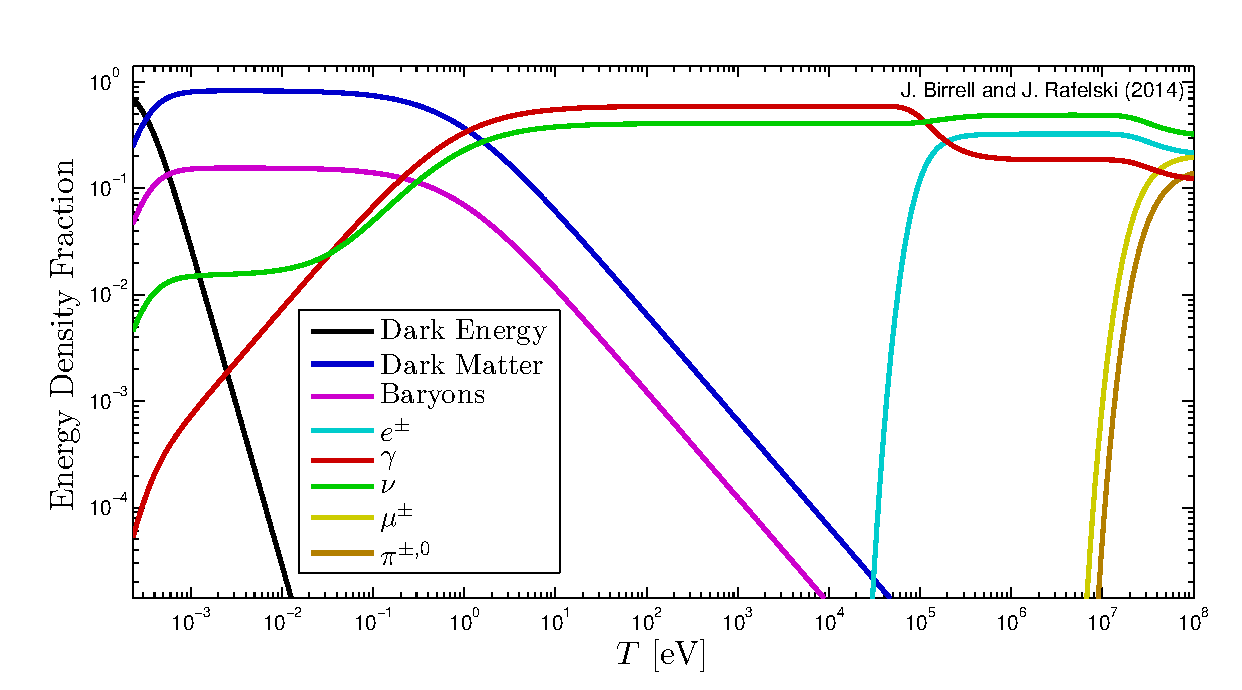
\includegraphics[height=7.6cm]{03-birrell/ErasOfUniverse/energy_densities_total.eps}}\label{fig:energy_frac}
\caption{Current era: $69\%$ dark energy, $26\%$ dark matter, $5\%$ baryons, $<1\%$ photons and neutrinos, $1$ massless and $2\times .1$ eV neutrinos (Neutrino mass choice is just for illustration.  Other values are possible).}
 \end{figure}
%%%%%%%%%%%%%%%%%%%%%%%%%%%%%%%%%%
In figure \ref{fig:energy_frac} we begin on the right at the end of the hadron era with the disappearance of muons and pions.  This constitutes a reheating period, with energy and entropy from these particles being transfered to the remaining $e^\pm$, photon, neutrino plasma.  Continuing to $T=O(1)$ MeV, we come to the annihilation  of $e^\pm$ and the photon reheating period.  Notice that only the photon energy density fraction increases here.  As discussed above, a common simplifying assumption is that neutrinos are already decoupled at this time and hence do not share in the reheating process, leading to a difference in photon and neutrino temperatures \req{T_nu_T_gamma}.

After passing through a long period, from $T=O(1)$ MeV until $T=O(1)$ eV, where the energy density is dominated by photons and free-streaming neutrinos, we then come to the beginning of the matter dominated regime, where the energy density is dominated by dark matter and baryonic matter.  This transition is the result of the redshifting of the photon and neutrino energy, $\rho\propto T^4$, whereas for non-relativistic matter $\rho\propto a^{-3}\propto T^3$.  Note that our inclusion of neutrino mass causes the leveling out of the neutrino energy density fraction during this period, as compared to the continued redshifting of the photon energy.

Finally, as we move towards the present day CMB temperature of $T_{\gamma,0}=0.235$ meV on the left hand side, we have entered the dark energy dominated regime.  For the present day values, we have used the fits from the Planck data \cite{Planck} of  $69\%$ dark energy, $26\%$ dark matter and $5\%$ baryons (and zero spatial curvature).  The photon energy density is fixed by the CMB temperature $T_{\gamma,0}$ and the neutrino energy density is fixed by $T_{\gamma,0}$ along with the photon to neutrino temperature ratio.  Both constitute $<1\%$ of the current energy budget.
In this chapter, we will introduce the fundamental concepts in cosmology for us to explore the properties of the Universe during the `first hour'. I will first present the standard cosmological Friedmann-Lemaitre-Robertson-Walker (FLRW) model, then introduce the general Fermi/Bose distribution with and its application in the early Universe. Finally I present an overview of Universe evolution from $300\,\mathrm{MeV}>T>0.02\,\mathrm{MeV}$.
The Natural unit $c=\hbar=k_{B}=1$ is used throughout the thesis for discussion.
\section{Textbook review: the standard FLRW-Universe model}
%In this section we will focus on the following:
%\begin{itemize}
%    \item The Robertson –Walker Universe
%    \item The Friedmann equation (Hubble %    \item The composition of the universe
%\end{itemize}
The Friedmann-Lemaitre-Robertson-Walker (FLRW) Universe is a theoretical model used widely to describe the cosmological evolution of the Universe. It is based on the cosmological principles which assumes homogeneity and isotropy of the Universe on large scales. In general, the FLRW metric can be written as
\begin{align}\label{metric}
ds^2=c^2dt^2-a^2(t)\left[ \frac{dr^2}{1-kr^2}+r^2(d\theta^2+\sin^2\theta\,d\phi^2)\right].
\end{align}
The metric is characterized by the scale factor $a(t)$ which measures the size of the Universe as a function of time $t$. The geometric parameter $k$ identifies the Gaussian geometry of the spatial hyper-surfaces defined by co-moving observers. The metrics are qualitatively different depending on the value of $k$. We have $k=1$ which correspond to the closed Universe,  $k=0$ correspond to flat Universe, and $k=-1$ for open geometries of the Universe. Current observation of cosmic microwave background (CMB) anisotropy preferred value $k=0$~[\cite{Planck:2013pxb,Planck:2015fie,Planck:2018vyg}].
%%%%%%%%%%%%%%%%%%%%%%%%
\section{Particles and plasma in the Universe} \label{Introduction}
%{Introduction to cosmology and overview}
In this chapter, we will introduce the fundamental concepts in cosmology for us to explore the properties of the Universe during the `first hour'. I will first present the standard cosmological Friedmann-Lemaitre-Robertson-Walker (FLRW) model, then introduce the general Fermi/Bose distribution with and its application in the early Universe. Finally I present an overview of Universe evolution from $300\,\mathrm{MeV}>T>0.02\,\mathrm{MeV}$.
The Natural unit $c=\hbar=k_{B}=1$ is used throughout the thesis for discussion.
%{Introduction\daggerfootnote{This chapter has been published previously as \citet{Gottbrath1999}.}}

%~~~~~~~~~~~~~~~~~~~~~~~~~~~~~~~~~~~~~~~~~~~~~~~~~
%The modern observation in cosmology has demonstrated that the observed universe is highly symmetric in its large-scale structure and 

%~~~~~~~~~~~~~~~~~~~~~~~~~~~~~~~~~~~~~~~~~~~~~~~~~

\subsection{Approaching equilibrium: Fermi/Bose distributions}

In the early Universe, the reaction rates of particles in the cosmic plasma were much greater than the Universe expansion rate $H$. Therefore, the local thermal equilibrium has been maintained. Assuming the particles are in thermal equilibrium, the dynamical information can be obtained from the single-particle distribution function. The general relativistic covariant Fermi/Bose momentum distribution can be written as
\begin{align}
f_{F/B}(\Upsilon_i,p_i)=\frac{1}{\Upsilon^{-1}_i\exp{\left[(u\cdot p_i-\mu_i)/T\right]}\pm1}
\end{align}
where the plus sign applies for fermions, and the minus sign for bosons. The Lorentz scalar $(u_i\cdot p_i)$ is a scalar product of the particle four momentum $p^\mu_i$ with the local four vector of velocity $u^\mu$. In the absence of local matter flow, the local rest frame is the laboratory frame 
\begin{align}
u^\mu=\left(1,\vec{0}\right),\,\,\,\,\,\,\,\,\, p^\mu_i=\left(E_i,\vec{p}_i\right).
\end{align}  
The parameter $\Upsilon_i$ is the fugacity of a given particle which describes the pair density and it is the same for both particles and antiparticles. For $\Upsilon_i=1$ the distribution maximizes the entropy content at a fixed particle energy. The parameter $\mu_i$ is the chemical potential for a given particle which is associated to the density difference between particles and antiparticles. 

In general there are two types of chemical equilibriums associated with the chemical parameters $\Upsilon$ and $\mu$. We have:
\begin{itemize}
\item Absolute chemical equilibrium:\\
The absolute chemical equilibrium is the level to which energy is shared into accessible degrees of freedom, e.g. the particles can be made as energy is converted into matter.
The absolute equilibrium is reached when the phase space occupancy approaches unity $\Upsilon\to1$. 
 \item Relative chemical equilibrium:\\
 The relative chemical equilibrium is associated with the chemical potential $\mu$ which involves reactions that distribute a certain already existent element/property among different accessible compounds. 
 \end{itemize}
The dynamics of absolute chemical equilibrium, in which energy can be converted to and from particles and antiparticles, is especially important. The consequences for the energy conversion to from particles/antiparticle can be seen in the first law of thermodynamics by introducing the general chemical potential $\mu_N$ for particle and $\mu_{\bar{N}}$ for antiparticle as follows:
\begin{align}
\mu_N\equiv\mu+T\ln\Upsilon,\qquad{\mu_{\bar{N}}}\equiv{-\mu}+T\ln\Upsilon.
\end{align}
Then the first law of thermodynamics can be written as
\begin{align}
dE&=-PdV+TdS+{\mu_N}dN+{\mu_{\bar{N}}}d{\bar{N}}
\\&=-PdV+TdS+{\mu}(dN-d{\bar{N}})+T\ln{\Upsilon}(dN+d{\bar{N}}).
\end{align}
It shows that the chemical potential $\mu$ is the energy required to change the difference between particles and antiparticles, and the $T\ln\Upsilon$ is the energy required to change the total number of particle and antiparticle, and the fugacity $\Upsilon$ is the parameter to adjust the energy.

\subsubsection{Boltzmann equation and particle freeze-out}
The Boltzmann equation describes the evolution of distribution function f in phase space. The Boltzmann equation in the FLRW universe can be written as
\begin{align}
\frac{\partial f}{\partial t}-\frac{\left(E^2-m^2\right)}{E}H\frac{\partial f}{\partial E}=\frac{1}{E}\sum_{q}\mathcal{C}_q[f],
\end{align}
where $H=\dot{a}/a$ is the Hubble parameter. Due to homogeneity and isotropy of the Universe, the distribution function depends on time $t$ and energy $E=\sqrt{p^2+m^2}$ only. The collision term $\sum_qC_q$ represents all elastic and inelastic interactions and $q$ labels the corresponding physical process. In general, the collision term is proportional to the relaxation time for given collision as follows \cite{ANDERSON1974466}
\begin{align}
\frac{1}{E}\mathcal{C}_q[f]\propto\frac{1}{\tau_{rel}}
\end{align}
where $\tau_{rel}$ is the relaxation time for the reaction, which is on the order of magnitude of time for the reaction to reach chemical equilibrium. 


As the Universe expands, the collision term in the Boltzmann equation competes with the Hubble term. In general, a given particle freeze-out from the cosmic plasma when its interaction rate $\tau_{rel}^{-1}$ becomes smaller than the Hubble expansion rate
\begin{align}
H\geqslant\tau_{rel}^{-1}.
\end{align}
When this happens, the particle's interactions are not rapid enough to maintain thermal distribution, either because the density of particles becomes so low that the chances of any two particles meeting each other becomes negligible, or because the particle energy becomes too low to interact. The freeze-out process can be categorized into three distinct stages based on the type of freeze-out interactions, we have~\cite{Birrell:2012gg,Rafelski:2023emw}:

\begin{itemize}
\item Chemical freeze-out :\\
As the Universe expands and the temperature drops, the rate of the inelastic scattering (e.g. production and annihilation reaction) that maintain the equilibrium density becomes smaller than the expansion rate. At this point, the inelastic scattering ceases, and a relic population of particles remain. Prior to the chemical freeze-out temperature, number changing processes are significant and keep the particle in thermal equilibrium, implying that the distribution function has the usual Fermi-Dirac form 
\begin{equation}\label{equilibrium}
f_{th}(t,E)=\frac{1}{\exp[(E-\mu)/T]+1},\qquad \text{ for } T(t)> T_{ch}.
\end{equation}
where $T_{ch}$ represents the chemical freeze-out temperature.


\item Kinetic freeze-out:\\
After chemical freeze-out, particles  still scatter elastically from other particles and keep thermal equilibrium in the primordial plasma. As the temperature drops, the rate of elastic scattering reaction that maintain the thermal equilibrium become smaller than the expansion rate. At that time, elastic scattering processes cease, and the relic particles do not interact with other particles in the primordial plasma anymore. Before the kinetic freeze-out, the distribution function has the form
\begin{equation}\label{kinetic_equilib}
f_k(t,E)=\frac{1}{\Upsilon^{-1}\exp[(E-\mu)/T]+1},\qquad \text{ for }T_f< T(t)< T_{ch},
\end{equation}
where $T_f$ represents the kinetic freeze-out temperature. The generalized fugacity $\Upsilon(t)$ controls the occupancy of phase space and is necessary once $T(t)<T_{ch}$ in order to conserve particle number.


\item{Free streaming:}\\
After kinetic freeze-out, the particles have fully decoupled from the primordial plasma, and thereby ceased influencing the dynamics of the Universe and become free-streaming. The Einstein-Vlasov equation can be solved \cite{choquet2008general} and the free-streaming momentum distribution can be written as \cite{Birrell:2012gg}
\begin{equation}\label{free_stream_dist}
f_{fs}(t,E)=\frac{1}{\Upsilon^{-1}\exp{\left[\sqrt{\frac{E^2-m^2}{T_{fs}^2}+\frac{m^2}{T^2_f}}-\frac{\mu}{T_f}\right]+1}},\quad T_{fs}(t)=\frac{T_fa(t_k)}{a(t)},
\end{equation}
where the free-streaming effective temperature $T_{fs}$ is obtained by redshifting the temperature at kinetic freeze-out. If a massive particle (e.g. dark matter) freeze-out from cosmic plasma in the nonrelativistic regime, $m\gg T_f$. We can use the
Boltzmann approximation, and the free-streaming distribution for nonrelativistic particle becomes
\begin{align}
&f^B_{fs}(t,p)=\Upsilon\,e^{-(m+\mu)/T_f}\exp\left[-\frac{1}{ T_{eff}}\frac{p^2}{2m}\right],\quad T_{eff}=\left(\frac{a(t_f)}{a(t)}\right)^2T_f,
\end{align}
where we define the effective temperature $T_{eff}$ for massive free-streaming particle. In this scenario, the effective temperature for massive particles decreases faster than the Universe temperature cools. It's worth emphasizing the different temperatures between cold free-streaming particles and hot cosmic plasma would affect the evolution of the early Universe and require more detailed study. 
\end{itemize}

The division of the freeze-out process into these three regimes is a simplification. However, it is a very useful approximation in the study of cosmology~\cite{Mangano:2005cc,Birrell:2014gea}. For detailed discussion, see \cite{Birrell:2012gg,Rafelski:2023emw}.




\subsection{Thermodynamics of the Early Universe}
In the case of local thermal equilibrium, the laws of thermodynamics can provide a framework for understanding the behavior of particle's energy density, pressure, number density and entropy in the early Universe.

Using the relativistic covariant Fermi/Bose momentum distribution, the corresponding energy density, pressure, and number densities for particle species $i$ are given by
\begin{align}
\rho_i&=g_i\int\!\!\frac{d^3p}{(2\pi)^3}Ef_{F/B}=\frac{g_i}{2\pi^2}\!\int_{m_i}^\infty\!\!\!dE\,\frac{E^2\left(E^2-m_i^2\right)^{1/2}}{\Upsilon_i^{-1}e^{(E-\mu_i)/T}\pm 1},\label{energy_density}\\[0.2cm]
P_i&=g_i\int\!\!\frac{d^3p}{(2\pi)^3}\frac{p^2}{3E}f_{F/B}=\frac{g_i}{6\pi^2}\!\int_{m_i}^\infty\!\!\!dE\,\frac{\left(E^2-m_i^2\right)^{3/2}}{\Upsilon_i^{-1} e^{(E-\mu_i)/T}\pm 1},\label{Pressure_density}\\[0.2cm]
n_i&=g_i\int\!\!\frac{d^3p}{(2\pi)^3}f_{F/B}=\frac{g_i}{2\pi^2}\!\int_{m_i}^\infty\!\!\!dE\,\frac{E(E^2-m_i^2)^{1/2} }{\Upsilon_i^{-1}e^{(E-\mu_i)/T}\pm 1}
\label{number_density}
\end{align}
where $g_i$ is the degeneracy of the particle species. By including the fugacity parameter $\Upsilon_i$ allows us to characterize particle properties in nonchemical equilibrium situations.
On the other hand, the corresponding free-streaming energy density, pressure, and number densities can be written as
\begin{align}
\rho_i&=g_i\int\!\!\frac{d^3p}{(2\pi)^3}Ef_{fs}=\frac{g_i}{2\pi^2}\!\int_{m_i}^\infty\!\!\!dE\,\frac{E^2\left(E^2-m_i^2\right)^{1/2}}{\Upsilon_i^{-1}e^{\sqrt{p^2/T_{fs}^2+m_i^2 /T_f^2}-\mu_i/T_f}\pm 1},\label{free_energy_density}\\[0.2cm]
P_i&=g_i\int\!\!\frac{d^3p}{(2\pi)^3}\frac{p^2}{3E}f_{fs}=\frac{g_i}{6\pi^2}\!\int_{m_i}^\infty\!\!\!dE\,\frac{\left(E^2-m_i^2\right)^{3/2}}{\Upsilon_i^{-1}e^{\sqrt{p^2/T_{fs}^2+m_i^2 /T_f^2}-\mu_i/T_f}\pm1},\label{free_Pressure_density}\\[0.2cm]
n_i&=g_i\int\!\!\frac{d^3p}{(2\pi)^3}f_{fs}=\frac{g_i}{2\pi^2}\!\int_{m_i}^\infty\!\!\!dE\,\frac{E(E^2-m_i^2)^{1/2} }{\Upsilon_i^{-1}e^{\sqrt{p^2/T_{fs}^2+m_i^2 /T_f^2}-\mu_i/T_f}\pm1},
\label{free_number_density}
\end{align} 
which are different from the thermal equilibrium Eq.~(\ref{energy_density}), Eq.~(\ref{Pressure_density}), and Eq.~(\ref{number_density}), by replacing the mass by a time dependant effective mass $m\,T_{fs}(t)/T_f$ in the exponential.





Given the energy density, pressure, and number densities, the entropy density for particle species $i$ can be written as
\begin{align}\label{entropy}
\sigma_i=\frac{S_i}{V}=\left(\frac{\rho_i+P_i}{T}-\frac{\mu_i}{T}\,n_i\right).
\end{align}
In general the chemical potential is associated with the baryon number. Since the net baryon number density relative to the photon number density is of order $10^{-9}$. In this case, we can neglect the small chemical potential when calculating the total entropy density in the Universe. The total entropy density in the early Universe can be written as
\begin{align}
&\sigma=\sum_i\,\sigma_i=\frac{2\pi^2}{45}g^s_\ast\,T^3,\\
&g^s_\ast=\sum_{i=\mathrm{bosons}}g_i\left({\frac{T_i}{T_\gamma}}\right)^3B\left(\frac{m_i}{T_i}\right)+\frac{7}{8}\sum_{i=\mathrm{fermions}}g_i\left({\frac{T_i}{T_\gamma}}\right)^3F\left(\frac{m_i}{T_i}\right),
\end{align}
where $g^s_\ast$ counts the effective number of `entropy' degrees of freedom. The functions $B(m_i/T)$ and $F(m_i/T)$ are defined as
\begin{align}
&B\left(\frac{m_i}{T}\right)=\frac{45}{12\pi^4}\int^\infty_{m_i/T}\,dx\sqrt{x^2-\left(\frac{m_i}{T}\right)^2}\left[4x^2-\left(\frac{m_i}{T}\right)^2\right]\frac{1}{\Upsilon^{-1}_ie^x-1},\\
&F\left(\frac{m_i}{T}\right)=\frac{45}{12\pi^4}\frac{8}{7}\int^\infty_{m_i/T}\,dx\sqrt{x^2-\left(\frac{m_i}{T}\right)^2}\left[4x^2-\left(\frac{m_i}{T}\right)^2\right]\frac{1}{\Upsilon^{-1}_ie^x+1}.
\end{align}
In Fig.~\ref{EntropyDOF_Fig} we plot the $g^s_\ast$ as a function of temperature, the effect of particle mass threshold~\cite{Coc:2006rt} is considered in the calculation for all involved particles. When $T$ decreases below the mass of particle $T\ll m_i$, this particle species becomes nonrelativistic and the contribution to $g^s_\ast$ becomes negligible, creating the dependence on $T$ seen in Fig.\,\ref{EntropyDOF_Fig}.
%~~~~~~~~~~~~~~~~~~~~~~~~~~~~~~~~~~~~~~~~~~~~~~~~~~~~~~~~~~~~~~~~~~~~~~~~~~~~~~~~
\begin{figure}[t]
%\begin{center}
\centering
\includegraphics[width=\linewidth]
%{./plots/DOF_entropy.jpg}
{./plots/g_entropy.jpg}
\caption{The entropy degrees of freedom as a function of $T$ in the early Universe epoch after hadronization $10^{-2}\,\mathrm{MeV} \leqslant  T \leqslant 150 $\,MeV. When particle species becomes nonrelativistic $T\ll m_i$, the contribution to $g^s_\ast$ becomes negligible, as a result creating the dependence $g^s_\ast(T)$.The vertical lines represents the mass of particles: $m_e=0.511$ MeV, $m_\mu=105.6$ MeV, and pion average mass $m_\pi\approx138$ MeV. Adapted from thesis of C.T.Yang \cite{Yang:2024ret}.}
\label{EntropyDOF_Fig}  
\end{figure}
%~~~~~~~~~~~~~~~~~~~~~~~~~~~~~~~~~~~~~~~~~~~~~~~~~~~~~~~~~~~~~~~~~~~~~~~~~~~~~~~~


\subsubsection{Relation between time and temperature}
Considering the comoving entropy conservation, we have
\begin{align}
S=\sigma V\propto g^s_\ast T^3a^3=\mathrm{constant},
\end{align}
where $g^s_\ast$ is the entropy degree of freedom and $a$ is the scale factor. Differentiating the entropy with respect to time $t$ we obtain
\begin{align}
\left[\frac{\dot{T}}{g^s_\ast}\frac{dg^s_\ast}{dT}+3\frac{\dot{T}}{T}+3\frac{\dot{a}}{a}\right]g^s_\ast T^3a^3=0,\qquad \dot{T}=\frac{dT}{dt}.
\end{align}
Solving $dT/dt$ and taking the integral, the relation between time and temperature in early universe can be written as
\begin{align}\label{time}
t(T)=t_0-\int^T_{T_0}dT\frac{1}{HT}\left[1+\frac{T}{3g^s_\ast}\frac{dg^s_\ast}{dT}\right],\qquad H^2=\frac{8\pi G_N}{3}\rho_{tot}
\end{align}
where $T_0$ and $t_0$ represent the initial temperature and time respectively, $H$ is the Hubble parameter and $\rho_{tot}$ is the total energy density in early Universe. From Eq. (\ref{time}) we see that the cosmic time depends on the entropy degrees of freedom $g^\ast_s$, which are characterized by the relativistic components in the early Universe. In the temperature range we consider $300\,\mathrm{MeV}>T>0.02\,\mathrm{MeV}$ the Universe is radiation-dominated and $\Lambda$CDM model is not used in this epoch.

%~~~~~~~~~~~~~~~~~~~~~~~~~~~~~~~~~~~~~~~~~~~~~~~~~~~~~~~~~~~~~~~$

\subsubsection{The baryon-per-entropy density ratio}
An important assumption allowing us to explore the early Universe evolution is that following on the era of matter genesis both baryon and entropy content is conserved in the comoving volume. Both baryon and entropy density scale with the third power of the expansion parameter $a(t)$. Therefore the ratio of baryon number density to visible matter entropy density remains constant throughout the evolution of universe. We have
\begin{align}
\frac{n_B-n_{\overline{B}}}{\sigma}= \left.\frac{n_B-n_{\overline{B}}}{ \sigma}\right|_{t_0}=\mathrm{Const.}\;
\end{align}
The subscript $t_0$ denotes the present day condition, and $\sigma$ is the total entropy density.
The observation gives the present baryon-to-photon ratio ~\cite{ParticleDataGroup:2022pth} $5.8 \times 10^{-10} \leqslant(n_B-n_{\overline{B}})/n_\gamma\leqslant6.5\times10^{-10}$. This small value quantifies the matter-antimatter asymmetry in the present day Universe, and allows the determination of the present value of baryon per entropy ratio~\cite{Rafelski:2019twp,Fromerth:2002wb,Fromerth:2012fe}:
\begin{align}\label{BaryonEntropyRatio}
\left.\frac{n_B-n_{\overline{B}}}{ \sigma}\right|_{t_0}=\eta\left(\frac{n_\gamma}{\sigma_\gamma+\sigma_\nu}\right)_{\!t_0}\!\!\!\!=(8.69\pm0.05)\!\!\times\!\!10^{-11},\qquad \eta=\frac{(n_B-n_{\overline{B}})}{n_\gamma},
\end{align}
where the $\eta=(6.12\pm0.04)\times10^{-10}$~\cite{ParticleDataGroup:2022pth} is used in calculation. To obtain the ratio, we consider that the Universe today is dominated by photons and free-streaming massless neutrinos~\cite{Birrell:2012gg}, and $\sigma_\gamma$ and $\sigma_\nu$ are the entropy densities for photon and neutrino respectively. We have
\begin{align}
    \frac{\sigma_\nu}{\sigma_\gamma}=\frac{7}{8}\,\frac{g_\nu}{g_\gamma}\left(\frac{T_\nu}{T_\gamma}\right)^3\,\qquad\frac{T_\nu}{T_\gamma}=\left(\frac{4}{11}\right)^{1/3}
\end{align}
and the entropy-per-particle for massless bosons and fermions are given by~\cite{Fromerth:2012fe}
\begin{align}
s/n|_\mathrm{boson}\approx 3.60\,,\qquad
s/n|_\mathrm{fermion}\approx 4.20\,.
\end{align}
However, from the neutrino oscillation experiment, we know that the the neutrinos are not massless particles. 
The mass differences between neutrino mass eigenstates are~\cite{ParticleDataGroup:2022pth}:
\begin{align}
&\Delta{m}_{21}^2=7.39^{+0.21}_{-0.20}\times10^{-5}\,\mathrm{eV}^2,\\
&\Delta{m}_{32}^2=2.45^{+0.03}_{-0.03}\times10^{-3}\,\mathrm{eV}^2.
\end{align}
Neutrino mass eigenvalues can be ordered in the normal mass hierarchy ($m_1\ll m_2<m_3$) or inverted mass hierarchy ($m_3\ll m_1<m_2$). All three mass states remained relativistic until the temperature dropped below their rest mass. These results allow for the possibility that one mass eigenstate or two mass eigenstates of neutrinos may become non-relativistic today, which can affect the baryon-per-entropy ratio.




%~~~~~~~~~~~~~~~~~~~~~~~~~~~~~~~~~~~~~~~~~~~~~~~~~~~



\subsubsection{Nonequilibrium: departure from detailed balance}
Thermal equilibrium implies both chemical equilibrium (particles abundances are balanced) and kinetic equilibrium (energy is evenly distributed). In chemical equilibrium, the rates of the forward and reverse reactions are equal, resulting in a balance between production and annihilation/decay rates, which is called detailed balance. The chemical non-equilibrium can be achieved by breaking this detailed balance and leading to change in particle abundance over time. On the other hand, kinetic equilibrium is usually established much quicker and has less impact on the actual particle abundances.
The chemical nonequilibrium condition is more important than the kinetic equilibrium because it relates to the arrow of time for the particle reactions. 

The chemical nonequilibrium conditions in the early Universe are of general interest: they are understood to be prerequisite for the arrow of time dependent processes to take hold in the Hubble expanding Universe. The arrow of time plays an important role in the evolution of the early Universe, for example:
 1.) The Big Bang Nucleosynthesis (BBN)~\cite{Pitrou:2018cgg,Kolb:1990vq,Dodelson:2003ft,Mukhanov:2005sc}  the synthesis of light elements of  e.g. D, $^3$He, $^4$He, and $^7$Li are produced at temperatures around $86\,\mathrm{keV}>T_{BBN}>50\,\mathrm{keV}$. 
 2.) Baryogenesis is believed to occur at or before the Universe underwent electroweak phase transition~\cite{Kolb:1990vq} at a temperature $T\simeq 130$\, GeV, which generates the excess of baryon number compared to anti-baryon number in order to create the observed baryon number today.

When Universe expands and temperature cools down, the chemical non-equilibrium can be achieved by breaking the detailed balance between particle production reaction and annihilation/decay as follows:

1.) The particle production rate becomes slower than the rate of Universe expansion and the production reaction freezeout. Once the production reactions freezeout from the cosmic plasma, the corresponding detailed balance is broken and particle abundance decrease via the decay/annihilation reactions.
 

2.) The non-equilibrium can also be achieved when the production reaction slows down and is not able to keep up with decay/annihilation reaction. In this case, the Hubble expansion rate is much longer than the decay and production rate and is not relevant to the nonequilibrium process. The key factor is competition between production and decay/annihilation  which can result in chemical nonequilibrium in the early Universe.

\noindent We will investigate the nonequilibrium situation for bottom quarks and strang quarks in early universe and their application in Chapter~\ref{Bottom} and Chapter~\ref{Strangeness}, respectively.  

\section{Quark and Hadron Universe}\label{part2}
%%%%%%%%%%%%%%%%%%%%%%%%%%%%%%%%%%%%%%%%%
\subsection{Heavy particles in QGP epoch}
\label{HiggsQGP}
%%%%%%%%%%%%%%%%%%%%%%%%%%%%%%%%%%%%
\para{Matter phases in extreme conditions}
This section will be focused on a few examples of interest to cosmological context. In the temperature domain below electroweak boundary near $T=130$\,GeV we explore in preliminary fashion novel and interesting physical processes. We will consider the Higgs meson and the heavy quarks $t,b,c$ with emphasis on bottom quarks. We will show that the bottom quarks can deviate from chemical equilibrium $\Upsilon\neq 1$ by breaking the detailed balance between production and decay reactions. It is easy to see considering temperature scaling and additional degrees of freedom that the energy density of matter near to electroweak phase transition is a stunning 12 orders of magnitude greater compared to the benchmark we discussed for QGP-hadronization, see~\req{endensval}.
 
The dynamical bottom $ b,\bar b$-quark pair abundance depends on the competition between the strong interaction two gluon fusion process into $b\bar b$-pair and weak interaction decay rate of these heavy quarks. This lead to the off-equilibrium phenomenon of the bottom quark freeze-out in abundance near the hadronization temperature as discussed in Ref.\,\cite{Yang:2020nne} and below. Here we further argue that the same unusual situation could exist for any other heavy particle in QGP at a temperature well below their mass scale. We study as an example the abundance of the Higgs particle at condition $m_H\gg T$. Higgs is a particularly interesting case due to its special position in the particle ZOO and a narrow width.

We also explore the properties of hadronic phase after hadronization with special emphasis on gaining an understanding about the strangeness $s,\bar s$ content of the Universe which persists to unexpectedly low temperature. Many of the methods we use in this context were developed in order to understand the properties of strongly interacting QGP formed in relativistic \ie\ high-energy heavy-ion \ie\ nuclear collision experiments. Such experimental program is in progress at the Relativistic Heavy Ion Collider (RHIC) at BNL-New York\index{BNL!RHIC} and the Large Hadron Collider (LHC) at CERN\index{CERN!LHC}. 

Let us remind the reasons why the dynamics of particles and plasma in the primordial Universe differs greatly from the laboratory environment. We focus here on the case of QGP-hadron phase boundary but a similar tabular list applies to other era boundaries:\index{Big-Bang!difference with laboratory}
\begin{enumerate} 
\item The primordial Big-Bang QGP epoch lasts for about $20\,\mu$s. On the other hand, the QGP formed in collision micro-bangs has a lifespan of around $10^{-23}$\,s. 
\item In the primordial Universe the microscopic transformation of quarks into hadrons proceeded through creation of the so called mixed phase allowing for local equilibration and a full relaxation of strongly interacting degrees of freedom during about $10\,\mu$s~\cite{Fromerth:2002wb}. Current lattice QCD models predict a smooth transformation. The transformation in the laboratory is much closer to what can be called explosive and sudden conversion of quarks into hadronic (confined) degrees of freedom~\cite{Rafelski:2000by}. Such a situation can mimic phenomena usually observed in a true phase transition of first order.
\item Half of the degrees of freedom present in the Universe (charged leptons, photons, neutrinos) are not part of the thermal laboratory micro-bang.
\item Experimental reach today is at and below $T\simeq 0.5$\,GeV allowing to explore the hadronization process of the QGP but not the heavy particle (H,W,Z,$t$) content, $b$ and $c$ quarks are difficult to study. 
\item Though the baryon content of the laboratory QGP is very low it is probably also much higher compared to the observed baryon asymmetry in the Universe. 
\end{enumerate}
 
%%%%%%%%%%%%%%%%%%%%%%%%%%%%%%%%%%%
\para{Higgs equilibrium abundance in QGP} 
We would like to show that it is of interest to study the Higgs particle dynamics at relatively late stage of Universe evolution. This is an ongoing project which is described here for the first time. We are now considering in the primordial Universe the temperature range $10\,\mathrm{GeV}>T>1\,\mathrm{GeV}$, and recall the mass of the Higgs particle $m_H\simeq 125\GeV$. Therefore the number density of the Higgs can be written using the relativistic Boltzmann limit
\begin{align}
n_{H}=\frac{\Upsilon_H}{2\pi^2}T^3\left(\frac{m_H}{T}\right)^2 K_2(m_H/T)\,.
\end{align}\index{Higgs!particle abundance}

We are interested to compare the abundance of the Higgs particle to the net abundance of baryon excess over antibaryons to determine at which temperature the Higgs particle yield drops below this tiny Universe asymmetry. Our interest derives from the question how far down in temperature a baryon number breaking Higgs decay could be of relevance. Clearly, once the Higgs yield falls far below baryon asymmetry it would be difficult to argue it can contribute to grow the baryon asymmetry in the Universe. Moreover, comparing to baryon asymmetry seems to be a reliable measure of more general physical relevance, after all, our present Universe structure derives from this small asymmetry probably developed in the primordial epoch we explore here. 
 
The density between Higgs and baryon asymmetry (quark-antiquark asymmetry) can be written as
\begin{align}
\frac{n_H}{(n_B-n_{\bar{B}})}=\frac{n_{H}}{s_{tot}}\,\left(\frac{s_{tot}}{n_B-n_{\bar{B}}}\right)=
\frac{n_{H}}{s_{tot}}\left[\frac{s_{\gamma,\nu}}{n_B-n_{\bar{B}}}\right]_{t_0}\,.
\end{align}
Assuming no `late' baryon genesis and entropy conserving Universe expansion, we introduce in \req{BaryonEntropyRatio} in the last equality the present day value of baryon per entropy ratio. The entropy density $s_{tot}$ in QGP can be obtained employing the entropic degrees of freedom $g^s_\ast$, \req{eq:entg} and~\rf{EntropyDOF:Fig}
\begin{align}
 &s_{tot}=\frac{2\pi^2}{45}g^s_\ast T_\gamma^3,\qquad g^s_\ast=\sum_{i=\mathrm{g},\gamma}g_i\left({\frac{T_i}{T_\gamma}}\right)^3+\frac{7}{8}\sum_{i=l^\pm,\nu,u,d}g_i\left({\frac{T_i}{T_\gamma}}\right)^3\,.
\end{align}
The entropy content to a good approximation is dominated by all effectively massless particles at given temperature in QGP. 

The baryon-to-photon density ratio $\eta$ today is bracketed by $5.8\times10^{-10} \leqslant\eta\leqslant6.5\times10^{-10}$ \cite{ParticleDataGroup:2018ovx}, a more precise value $\eta=(6.12\pm0.04)\times10^{-10}$~\cite{ParticleDataGroup:2022pth} is used in our study. This observed value is the evidence of baryon asymmetry and quantifies the matter-antimatter asymmetry in the Universe.\index{baryon!photon ratio}

The density ratio between Higgs and baryon asymmetry for the case of chemical equilibrium $\Upsilon_H=1$ is seen in~\rf{HiggsDensity:fig}. At temperature $T=5.7\GeV$ this ratio is equal to unity. This implies that Higgs decay processes could populate and influence the baryon asymmetry down to this relatively low temperature scale. 

%%%%%%%%%%%%%%%%%%%%%%%%%%%%%%%%%%%%%%%%%%%%%%%%%%%%%%%%%%%%%%%%%%
\begin{figure}
\centerline{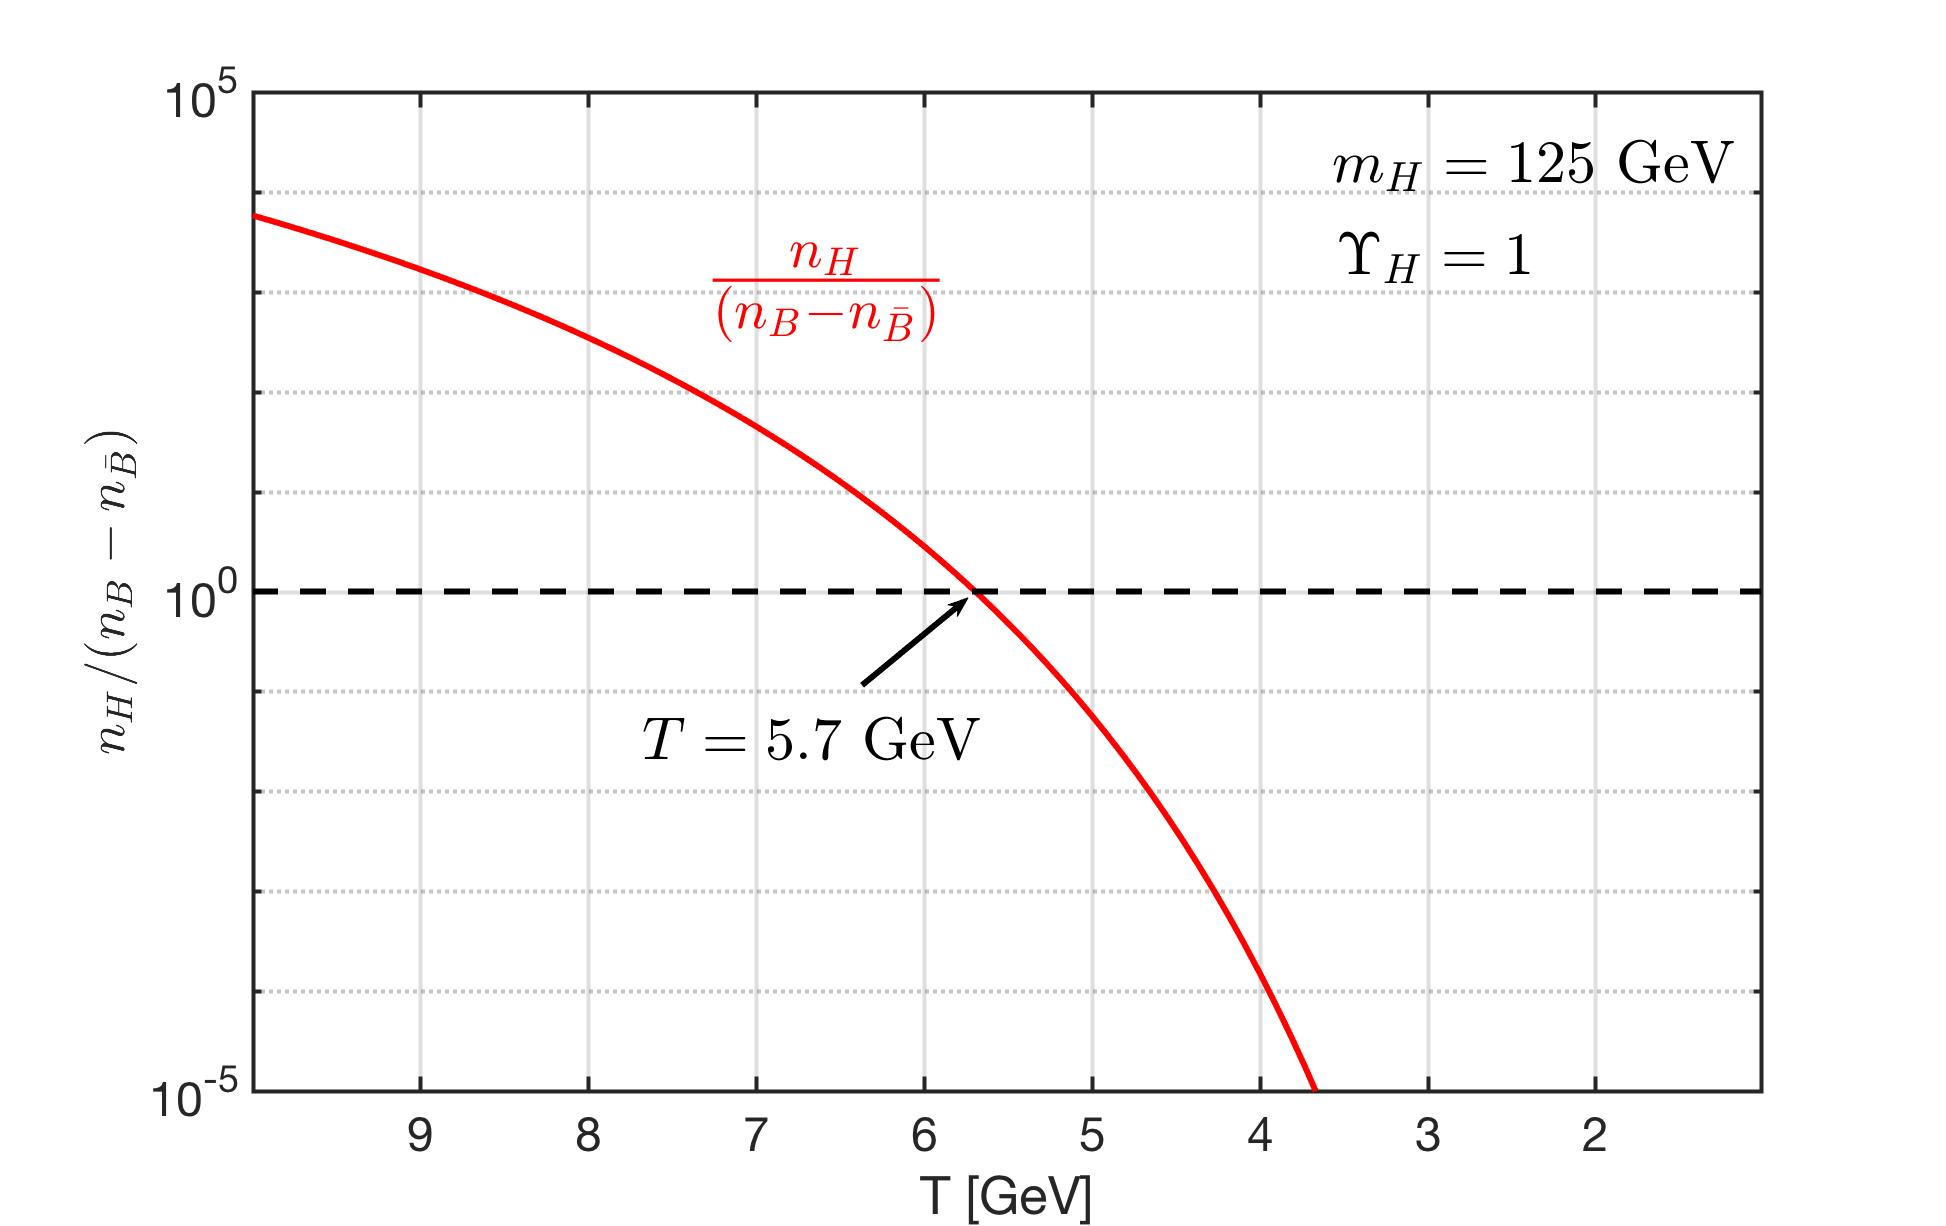
\includegraphics[width=0.9\linewidth]{./plots/HiggsDensityRatio}}
\caption{The ratio between Higgs density $n_H$ and baryon asymmetry density $n_B-n_{\bar B}$ as a function of temperature $T$ assuming chemical Higgs equilibrium $\Upsilon_H=1$ and present day entropy per baryon. Both densities are equal (horizontal line) at the temperature $T=5.7\GeV$. \radapt{Yang:2024ret}}
\label{HiggsDensity:fig} 
\end{figure}
%%%%%%%%%%%%%%%%%%%%%%%%%%%%%%%%%%%%%%%%%%%%%%%%%%%%%%%%%%%%%%%%%%%

%%%%%%%%%%%%%%%%%%%%%%%%%%%%
\para{Baryon asymmetry and Sakhraov conditions}\index{Sakharov conditions!baryogenesis}
The small value of the baryon asymmetry in the Universe could be interpreted as simply due to the initial conditions in the Universe. However, in the current standard cosmological model, it is believed that the inflation event can erase any pre-existing asymmetry between baryons and anti-baryons. In this case, we need a dynamic baryogenesis process to generate excess of baryon number compared to anti-baryon number in order to create the observed baryon number today.

The precise epoch responsible for the observed matter genesis $\eta$ in the primordial Universe has not been established yet. Several mechanisms have been proposed to explain baryogenesis with investigations typically focusing on the temperature range between GUT phase transition $T_\mathrm{G}\simeq10^{16}\,\mathrm{GeV}$ and the electroweak phase transition near $T_\mathrm{W}\simeq130\,\mathrm{GeV}$~\cite{Kuzmin:1985mm,Kuzmin:1987wn,Arnold:1987mh,Kolb:1996jt,Riotto:1999yt,Nielsen:2001fy,Giudice:2003jh,Davidson:2008bu,Morrissey:2012db}.

In following we present arguments that the Sakharov conditions~\cite{Sakharov:1967dj} for matter asymmetry to form also could appear during the QGP era: several heavy particles such as bottom quarks and including the Higgs as described above can fulfill nonequilibrium requirement. We will study below in more detail the bottom case and argue for the Higgs case. Other cases are possible.

In 1967, Andrei Sakharov formulated the three conditions necessary to permit baryogenesis in the primordial Universe~\cite{Sakharov:1967dj} and in 1991 he refined the three conditions as follows~\cite{Sakharov:1988vdp}:
\begin{itemize}
 \item Absence of baryonic charge conservation 
 \item Violation of CP-invariance
 \item Non-stationary conditions in absence of local thermodynamic equilibrium
\end{itemize}
 
In regard to first Sakharov condition: By assumption there is no initial asymmetry in baryon number in the Universe. Toady it is argued that an initial asymmetry could not survive the inflationary expansion. Furthermore ad-hoc Big-Bang baryon-antibaryon inherent asymmetry seems less attractive. In short we believe that the asymmetry between baryons and anti-baryons we observe requires dynamic process and the presence of baryon number non-conserving reactions. 

The other option, an interaction which favors agglomerations of same `sign' baryonic matter creating large domains in the Universe with small baryon-antibaryon asymmetry has never taken hold: We recall that the laws of physics favor opposite outcome, the elementary antimatter is eclectically attracted to matter. Neutral composite baryonic particles present in era in which antimatter is present (e.g. neutrons, $\Lambda(uds)$, charmed baryons etc., emerging just after QGP hadronization) deserve a second look on this account.

The second Sakharov condition requiring $CP$ violation assures us that we can recognize in universal manner the difference between matter and antimatter. Clearly, we could not enhance one form with reference to the other without being able to tell matter from antimatter. CP violation is allowing us to share with another distant civilization that we are made of matter. A nice textbook discussion showing how to do this using Kaon system CP violation is offered by Perkins~\cite{Perkins:1982xb}.

The third Sakharov condition is a requirement for breaking of detailed balance condition: It is evident that in thermal equilibrium, the net effect of baryogenesis processes is cancelled out by the detailed balance between forward and back-reactions. Space-time domains involving phase transitions harbor nonequilibrium thermal distributions leading to breaking of detailed balance. So far efforts to create consistent description of baryogenesis based on well studied electro-weak phase transition near $T=130$\,GeV has not been able to generate the observed baryon asymmetry. 

We distinguish kinetic (momentum distribution) and chemical (particle abundance) equilibrium. This is so since kinetic equilibrium is usually established much more quickly, while abundance yields are more difficult to establish, especially so for particles with masses in excess, or at least similar to ambient temperatures~\cite{Koch:1986ud,Birrell:2014gea}. This distinction has two relevant consequences: a) Detailed balance can arise also outside of strict chemical equilibrium condition which is seen in other physical environments, including the nucleo-synthesis processes in the Universe (BBN) and stars. b) There is a long lasting small violation of detailed balance related to the arrow of time introduced by the Universe expansion. c) Most promissing is for absence of stationary distribution is lack of kinetic equilibrium. 

Specifically for all heavy primordial particles including the top $t$ and bottom $b$ quarks, W and Z gauge bosons, and, the Higgs particle H we observe that when the Universe expands and temperature cools down well below the particle mass, the production process and decay processes create a stationary equilibrium with detailed balance outside of equilibrium. However, Universe expansion disturbs this creating non-stationary effects. Moreover, as we will argue just below, Higgs is an excellent candidate for non-stationary effects due to its small coupling to low mass particle plasma. Thus we interpret the third condition of Sakharov in our specific context as follows:
\begin{itemize}
\item Non-stationary conditions in absence of local thermodynamic equilibrium $\Longrightarrow$ Absence of detailed balance associated with nonequilibrium yields and non-stationary particle momentum abundance evolution.
\end{itemize} 

We believe that the presence of chemical (abundance) nonequilibrium is a required condition for baryogenesis environment which extends the phenomenon to a much wider temperture domain beyond the electro-weak phase transition condition down to a temperature of a few GeV. This is one of our ongoing research challenges. We will use the case of bottom quarks to demonstrate the mechanism we are exploring.
 
%%%%%%%%%%%%%%%%%%%%%%%%%%%%%%%
\para{Production and decay of Higgs in QGP}
The Higgs particle is unique among heavy PP-SM particles also due to its stability: The total width is $\Gamma_H\simeq 2.5\,10^{-5}M_H$. This combines with the unexpected low value of $T=5.7\GeV$ of interest where the Higgs yield equals to the baryon asymmetry in the Universe. This motivates us to examine here in qualitative manner the dynamical abundance of the Higgs particle in the QGP epoch, seeking eventual non-stationary condition needed for baryogenesis 

The Higgs predominantly decays via the $W,Z$ decay channels as follows:
\begin{align}
H\longrightarrow WW^\ast\,. ZZ^\ast\longrightarrow\mathrm{anything}\,.
\end{align}
Here $W^\ast,Z^\ast$ represent the production of virtual off-mass-shell gauge bosons decaying rapidly into relevant particle pairs. Therefore once Higgs decays via this channel at least four particles are ultimately formed and there is no path back for $T\ll m_H$. This is so since the spectral energy of produced particles, $31\GeV$ is highly epithermal compared to the ambient plasma at the low temperature of interest near to $T\simeq 6\GeV$. Therefore a back-reaction production of Higgs cannot be in balance for chemical equilibrium yield. 

In the QGP epoch, the dominant production of the Higgs boson is the bottom quark pair fusion reaction: 
\begin{align}
b+\overline{b}\longrightarrow H\,,
\end{align}
which is the inverse to the important but by far not dominant decay process of $H\to b+\overline{b}$. This means that in first approximation the detailed balance Higgs yield is reached well below the chemical equilibrium.

However, there could be considerable deviation from kinetic momentum equilibrium as well. This is so since bottom fusion will in general produce a Higgs particle out of kinetic momentum equilibrium. A heavy particle immersed into a plasma of lighter particles requires many, many collisions to equilibrate the momentum distribution. This is a well known kinetic theory result. Moreover, the Higgs particle interacts weakly with all lower mass particles in QGP present at $T<10\GeV$. 

Higgs particle is by far the best candidate to fulfill the Sakharov non-stationary condition in the primordial Universe at a temperature range of interest to baryogenesis. A full dynamic study leading to proper understanding of the off-chemical and off-kinetic equilibrium non-stationary abundance of Higgs is one of near future projects we consider and is beyond the scope of this report. 

%%%%%%%%%%%%%%%%%%%%%%%%%%%%%%%%
\subsection{Heavy quark production and decay}
\label{sec:heavyQ}
%%%%%%%%%%%%%%%%%%%%%%%%%%%%%%%%%
\para{Heavy quarks in primordial QGP}\index{quark!abundance}
The primordial quark-gluon plasma (QGP) refers to the state of matter that existed in the primordial Universe, specifically for time $t\approx 20\, \mathrm{\mu s}$ after the Big Bang. At that time the Universe was controlled by the strongly interacting particles: quarks and gluons. In this chapter, we study the heavy bottom and charm flavor quarks near to the QGP hadronization temperature $0.3\,\mathrm{GeV}>T>0.15\,\mathrm{GeV}$ and examine the relaxation time for the production and decay of bottom/charm quarks then show that the bottom quark nonequliibrium occur near to QGP–hadronization and create the arrow in time in the primordial Universe.
 
In the QGP epoch, up and down $(u,d)$ (anti)quarks are effectively massless and provide along with gluons, some leptons, and photons the thermal bath defining the thermal temperature. Strange $(s)$ (anti)quarks are also found to be in equilibrium considering their weak, electromagnetic, and strong interactions, indeed this equilibrium continues in hadronic epoch until $T\approx13\MeV$~\cite{Yang:2021bko}. 

The massive top $(t)$ (anti)quarks couple to the plasma via the channel~\cite{ParticleDataGroup:2018ovx}
\begin{equation}
t\leftrightarrow W+b\,,\qquad \Gamma_t=1.4\pm0.2\,\mathrm{GeV}\,.
\end{equation}
As is well known, the width prevents formation of bound toponium states. Given the large value of $\Gamma_t$ there is no freeze-out of top quarks until $W$ itself freezes out. To address the top quarks in QGP, a dynamic theory for $W$ abundance is needed, a topic we will embark on in the future. 
 
The semi-heavy bottom $(b)$ and charm $(c)$ quarks can be produced by strong interactions via quark-gluon pair fusion processes, these quarks decay via weak interaction decays, their abundance depends on the competition between the strong interaction fusion processes at low temperature inhibited by the mass threshold, and weak decay reaction rates.

In the following we consider the temperature near QGP hadronization $0.3\,\mathrm{GeV}>T>0.15\,\mathrm{GeV}$, and study the bottom and charm abundance by examining the relevant reaction rates of their production and decay.
In thermal equilibrium the number density of light quarks can be evaluated in the massless limit, and we have\index{number density of quark}
\begin{align}\label{FermiN}
n_q=\frac{g_{q}}{2\pi^2}\,T^3 F(\Upsilon_q)\;, \quad F=\int_0^\infty \frac{x^2dx}{1+\Upsilon_q^{-1}e^x}\;,
\end{align}
where $\Upsilon_q$ is the quark fugacity. We have $ F(\Upsilon_q=1)=3\,\zeta(3)/2$ with the Riemann zeta function $\zeta(3)\approx1.202$.
The thermal equilibrium number density of heavy quarks with mass $m\gg T$ can be well described by the Boltzmann expansion of the Fermi distribution function, giving
\begin{align}\label{BoltzN}
n_{q}\!=\!\frac{g_{q}T^3}{2\pi^2}\sum_{n=1}^{\infty}\frac{(-1)^{n+1}\Upsilon_q^n}{n^4}\left(\frac{n\,m_{q}}{T}\right)^{\!2}\!K_2\left(\frac{n\,m_{q}}{T}\right),
\end{align} 
where $K_2$ is the modified Bessel functions of integer order `$2$'. In the case of interest, when $m\gg T$, it suffices to consider the Boltzmann limit and keep the first term $n=1$ in the expansion. The first term $n=1$ also suffices for both charmed $c$-quarks and bottom $b$-quarks, giving
\begin{align}
&n_{b,c}={\Upsilon_{b,c}\,}n^{th}_{b,c},\qquad n^{th}_{b,c}=\frac{g_{b,c}}{2\pi^2}\,T^3\left(\frac{m_{b,c}}{T}\right)^2\,K_2(m_{b,c}/T).
\end{align}
However, for strange $s$ quarks, several terms are needed. 

In~\rf{number_entropy_b002} we show the equilibrium ($\Upsilon=1$) bottom and charm number density per entropy density ratio as a function of temperature $T$. The $b$-quark mass parameters shown are $m_b=4.2\,\mathrm{GeV}$ (blue) dotted line, $m_b=4.7\,\mathrm{GeV}$ (black) solid line, and $m_b=5.2\,\mathrm{GeV}$ (red) dashed line. For $c$-quark $m_c=0.93\,\mathrm{GeV}$ (blue) dotted line, $m_c=1.04\,\mathrm{GeV}$ (black) solid line, and $m_c=1.15\,\mathrm{GeV}$ (red) dashed line. The entropy density is given by~\req{entropy} and only light particles contribute significantly. Thus the result we consider is independent of actual abundance of $c$, $b$ and other heavy particles. 

%%%%%%%%%%%%%%%%%%%%%%%%%%%%%%%%%%%%%%%
\begin{figure}
\centerline{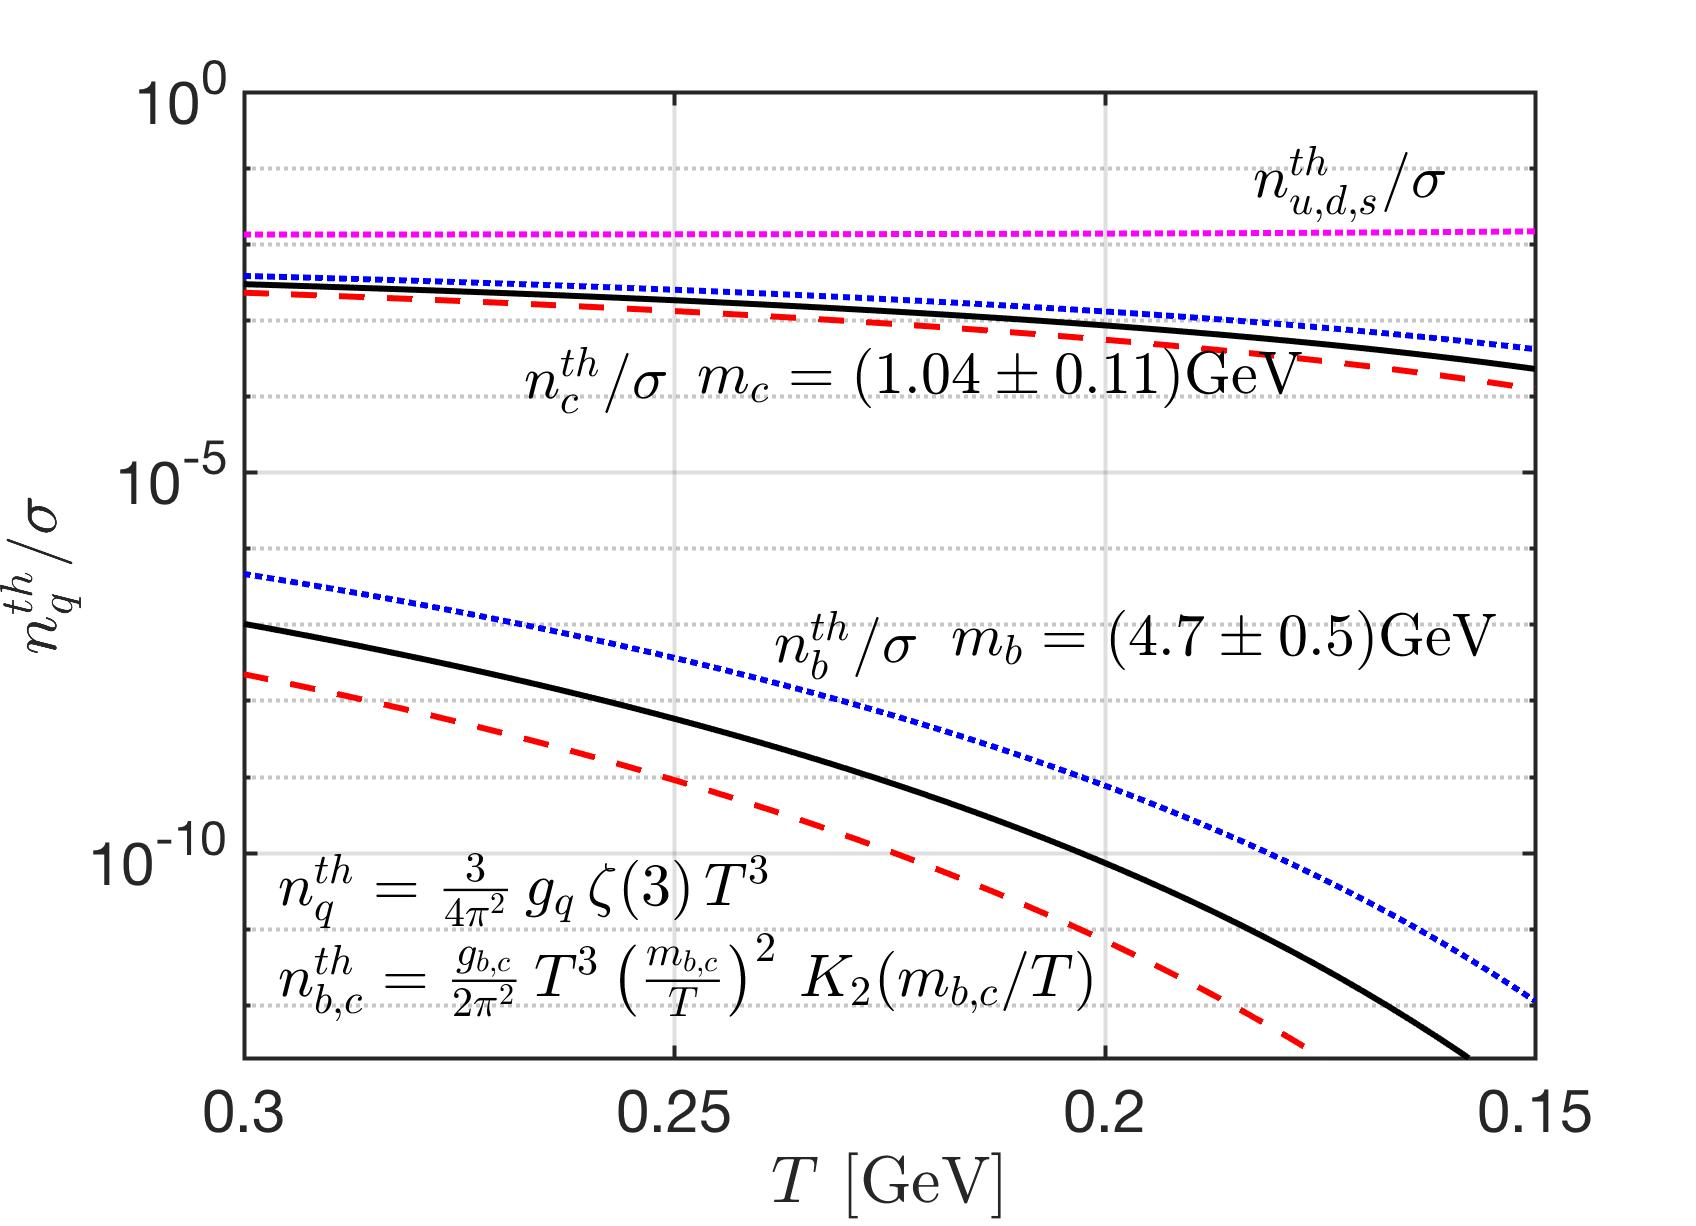
\includegraphics[width=0.9\linewidth]{./plots/bcQuarkDensity_new}}
\caption{
The equilibrium charm and bottom quark number density normalized by entropy density, as a function of temperature in the primordial Universe, see text for discussion of different mass values. \radapt{Yang:2024ret}}
\label{number_entropy_b002} 
\end{figure}
%%%%%%%%%%%%%%%%%%%%%%%%%%%%%%%%%%%%%%%%%%% 

The $m_b\simeq 5.2\,\mathrm{GeV}$ is a typical potential model mass used in modeling bound states of bottom, and $m_b=4.2,\,4.7\,\mathrm{GeV}$ is the current quark mass at low and high energy scales. In~\rf{number_entropy_b002} we see that the charm abundance in the domain of interest $0.3\,\mathrm{GeV}>T>0.15\,\mathrm{GeV}$ is about $10^4\sim 10^{9}$ times greater than the abundance of bottom quarks. This implies that the small $b$,$\bar b$ quark abundance is embedded in a large background comprising all lighter $u,d,s,c$ quarks and anti-quarks, as well as gluons $g$.

In the following we will calculate the production and decay rate for bottom and charm quarks and compare to the Universe expansion rate. We will show that in the epoch of interest to us the characteristic Universe expansion time $1/H$ is much longer than the lifespan and production time of the bottom/charm quark. In this case, the dilution of bottom/charm quark due to the Universe expansion is slow compare to the the strong interaction production, and the weak interaction decay of the bottom/charm. Any abundance nonequilibrium will therefore be nearly stationary.    

It is important for following analysis to know that the expansion of the Universe is the slowest process, allowing many microscopic reactions at a `fixed' temperature range $T$ to proceed. To show this we evaluate the Hubble relation to obtain $1/H$\,[s]
\begin{align}
H^2=\frac{8\pi G_N}{3}\left(\rho_\gamma+\rho_{\mathrm{lepton}}+\rho_{\mathrm{quark}}+\rho_{g,{W^\pm},{Z^0}}\right),
\end{align}
The effectively massless particles and radiation dominate particle energy density $\rho_i$ defining the speed of expansion of the Universe within  temperature range $130\, \mathrm{GeV}>T>0.15\,\mathrm{GeV}$; we have the following particles: photons, $8$ color charge gluons, $W^\pm$, $Z^0$, three generations of $3$ color charge quarks and leptons in the primordial QGP. The characteristic Universe expansion time constant $1/H$ is seen in~\rf{BCreaction:fig} below. In the epoch of interest to us $0.3\,\mathrm{GeV}>T>0.15\,\mathrm{GeV}$, the Hubble time $1/H\approx10^{-5}$ sec which is much longer than the microscopic lifespan and production time of the bottom and charm quarks we study 

%%%%%%%%%%%%%%%%%%%%%%%%%%%%%%%%%%%%%
\para{Quark production rate via strong interaction}\index{quark!production rate}
In primordial QGP, the bottom and charm quarks can be produced from strong interactions via quark-gluon pair fusion processes. For production, we have the following processes
\begin{align}
 q+\bar{q}&\longrightarrow b+\bar b,\qquad q+\bar{q}\longrightarrow c+\bar c,\\
 g+g&\longrightarrow b+\bar b,\qquad g+g\longrightarrow c+\bar c\,.
\end{align}

For the quark-gluon pair fusion processes\index{bottom quark!production rate}
%\begin{align}
% q+q&\longrightarrow b+\bar b,\qquad q+q\longrightarrow c+\bar c,\\
% g+g&\longrightarrow b+\bar b,\qquad g+g\longrightarrow c+\bar c,
%\end{align}
the evaluation of the lowest-order Feynman diagrams yields the cross sections~\cite{Letessier:2002ony}:
\begin{align}
&\sigma_{q\bar{q}\rightarrow b\bar{b},c\bar{c}}=\frac{8\pi\alpha_s^2}{27s}\left(1+\frac{2m_{b,c}^2}{s}\right)w(s),\,\qquad w(s)=\sqrt{1-{4m^2_{b,c}}/{s}},\\
&\sigma_{gg\rightarrow b\bar{b},c\bar{c}}=\!\frac{\pi\alpha_s^2}{3s}\bigg[\left(1\!+\!\frac{4m^2_{b,c}}{s}\!+\!\frac{m^4_{b,c}}{s^2}\right)\ln{\left(\frac{1+w(s)}{1-w(s)}\right)}\!-\!\left(\frac{7}{4}\!+\!\frac{31m^2_{b,c}}{4s}\right)w(s)\bigg],
\end{align} 
where $m_{b,c}$ represents the mass of bottom or charm quark, $s$ is the Mandelstam variable, and $\alpha_s$ is the QCD coupling constant. Considering the perturbation expansion of the coupling constant $\alpha_s$ for the two-loop approximation~\cite{Letessier:2002ony}, we have:
\begin{align}
\alpha_s(\mu^2)=\frac{4\pi}{\beta_0\ln({\mu^2/\Lambda^2})}\bigg[1-\frac{\beta_1}{\beta_0}\frac{\ln(\ln{(\mu^2/\Lambda^2)})}{\ln(\mu^2/\Lambda^2)}\bigg],
\end{align}
where $\mu$ is the renormalization energy scale and $\Lambda^2$ is a parameter that determines the strength of the interaction at a given energy scale in QCD. The energy scale we consider is based on required gluon/quark collisions above $b\bar b$ energy threshold, so we have $\mu=2m_b+T$. For the energy scale $\mu>2m_b$ we have $\Lambda=180\sim230\MeV$ ($\Lambda\approx205\MeV$ in our calculation), and the parameters $\beta_0=11-2n_f/3$, $\beta_1=102-38n_f/3$ with the number of active fermions $n_f=4$. 

%%%%%%%%%%%%%%%%%%%%%%%%%%%%%%%%%%%%%%%
\begin{figure} 
\centerline{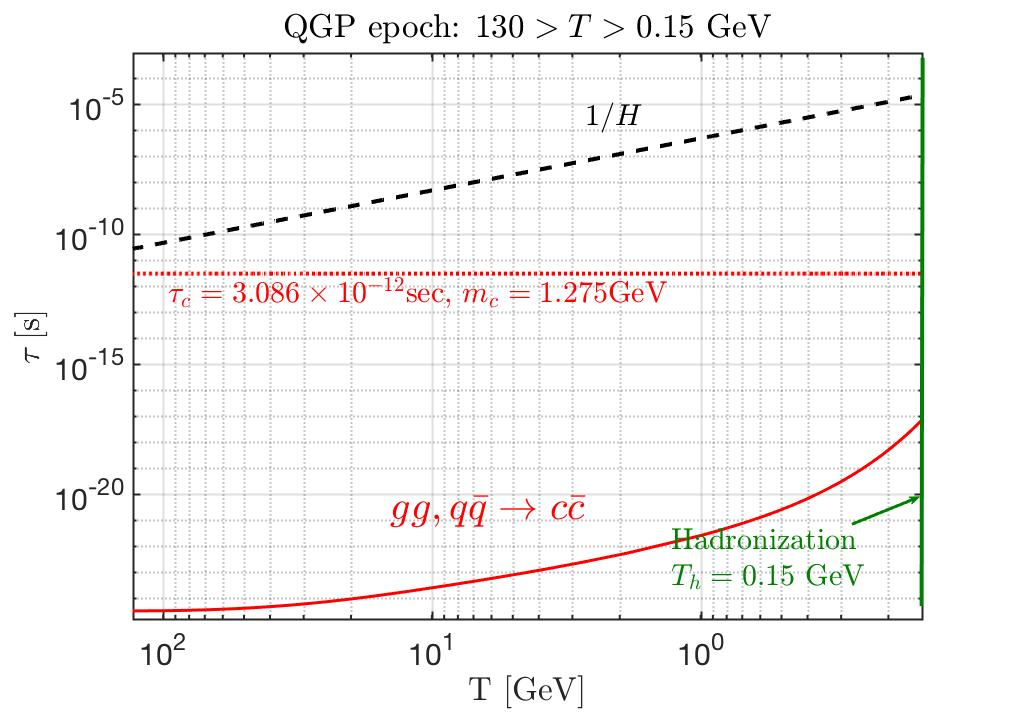
\includegraphics[width=0.9\linewidth]{./plots/CharmQuark_QGP.jpg}}
\centerline{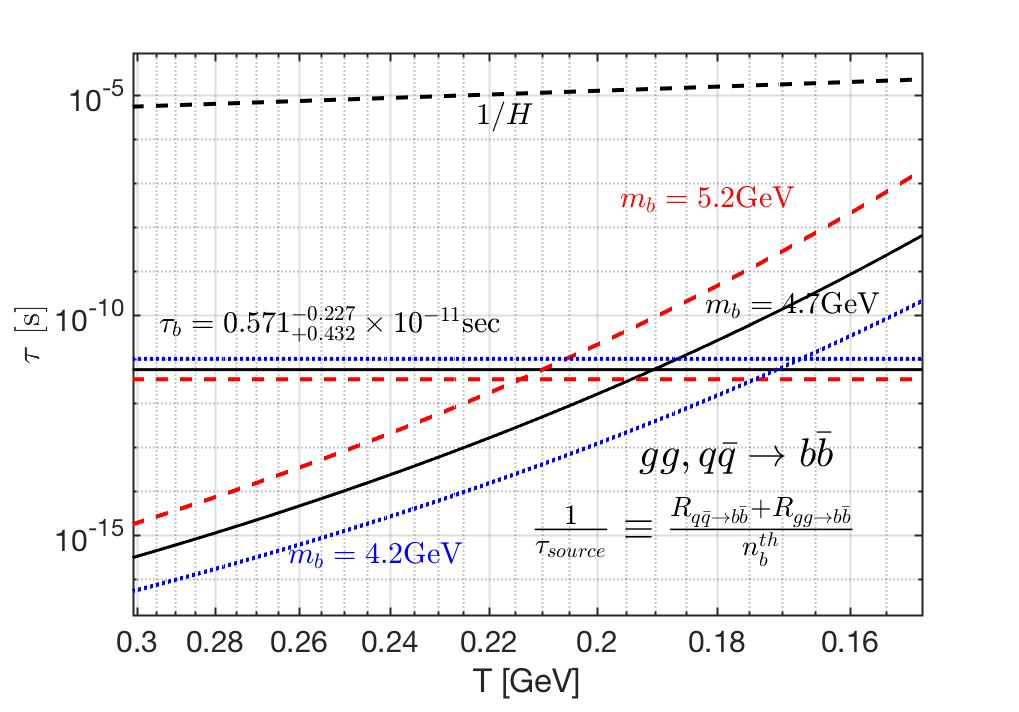
\includegraphics[width=0.9\linewidth]{./plots/BQuarkReactionTime_bottom.jpg}}
\caption{Comparison of Hubble time $1/H$, quark lifespan $\tau_{q}$, and characteristic time for production via quark, gluon pair fusion. The upper frame for charm $c$-quark in the entire QGP epoch $T$ rang; the lower frame for bottom $b$-quark amplifying the dynamic detail balance $T\simeq 200\MeV$. Both figures end at the hadronization temperature of $T_{H}\approx150\MeV$. See text for additional information. \cccite{Rafelski:2023emw}. \radapt{Yang:2024ret}}
\label{BCreaction:fig}
\end{figure}
%%%%%%%%%%%%%%%%%%%%%%%%%%%%%%%%%%%%%%%

In general the thermal reaction rate per unit time and volume $R$ can be written in terms of the scattering cross section as follows~\cite{Letessier:2002ony}:
\begin{align}
R\equiv\sum_i\int_{s_{th}}^\infty\!ds\,\frac{dR_i}{ds}=\sum_i\int_{s_{th}}^\infty\!ds\,\sigma_i(s)\,P_i(s),
\end{align}
where $\sigma_i(s)$ is the cross section of the reaction channel $i$, and $P_i(s)$ is the number of collisions per unit time and volume. Considering the quantum nature of the colliding particles (i.e., Fermi and Bose distribution) with the massless limit and chemical equilibrium condition ($\Upsilon=1$), we obtain~\cite{Letessier:2002ony}
\begin{align}
&P_i(s)=\frac{g_1g_2}{32\pi^4}\,\frac{T}{1+I_{12}}\frac{\lambda_2}{\sqrt{s}}\!\sum_{l,n=1}^{\infty}\!(\pm)^{l+n}\frac{K_1(\sqrt{lns}/T)}{\sqrt{ln}},\\
&\lambda_2\equiv\left[s-\left(m_1+m_2\right)^2\right]\,\left[s-\left(m_1-m_2\right)^2\right],
\end{align}
where $+$ is for boson and $-$ is for fermions, and the factor $1/(1+I_{12})$ is introduced to avoid double counting of indistinguishable pairs of particles. $I_{12}=1$ for identical pair of particles, otherwise $I_{12}=0$. Hence the total thermal reaction rate per volume for bottom quark production can be written as
\begin{align}
\label{Bquark_Source}
R^{\mathrm{Source}}_{b,c}=\int^\infty_{s_{th}}ds\,\bigg[\sigma_{q\bar{q}\rightarrow b\bar{b},c\bar{c}}\,P_q+\sigma_{gg\rightarrow b\bar{b},c\bar{c}}\,P_g\bigg]%=R_{q\bar{q}\rightarrow b\bar{b},c\bar{c}}+R_{gg\rightarrow b\bar{b},c\bar{c}}.
\end{align}
We introduce the bottom/charm quark relaxation time for the quark-gluon pair fusion as follows:
\begin{align}
\label{relaxation_time}
&{\tau_{b,c}^{\mathrm{Source}}}\equiv\frac{dn_{b,c}/d\Upsilon_{b,c}}{R^{\mathrm{Source}}_{b,c}}\;,\quad
\end{align}
where $dn_{b,c}/d\Upsilon_{b,c}=n^{th}_{b,c}$ in the Boltzmann approximation. The relaxation time is on the order of magnitude of time needed to reach chemical equilibrium. 

In~\rf{BCreaction:fig} we show the characteristic time for $b$ and $c$ quark strong interaction production. The $c$ quark (upper frame) is shown in the entire QGP temperature range. We note the vast 15 orders of magnitude difference between the Hubble time and the rate of production. This means that there will be very many microscopic cycles of charm production decay erasing any non-stationary effect.  For $b$ (lower frame) we restrict the view to temperature range in the domain of interest, $ 0.3\,\mathrm{GeV}>T> 0.15\,\mathrm{GeV}$. Three different masses $m_{b}=4.2\GeV$ (blue short dashes), $4.7\GeV$, (solid black), $5.2\GeV$ (red long dashes) for bottom quarks are shown. 
 
%%%%%%%%%%%%%%%%%%%%%%%%%%%%%%%%
\para{Quark decay rate via weak interaction}\index{quark!weak decay rate}
The bottom/charm quark decay via the weak interaction \index{bottom quark!decay rate} 
\begin{align}
 &b\longrightarrow c+l+\overline{\nu_l}, \qquad b\longrightarrow c+q+\bar{q},\\
&c\longrightarrow s+l+\overline{\nu_l},\qquad c\longrightarrow s+q+\bar{q}\,.
\end{align}

%\begin{align}
% &b\longrightarrow c+l+\nu_l, \qquad %b\longrightarrow c+q+\bar{q},\\
%&c\longrightarrow s+l+\nu_l,\qquad c\longrightarrow s+q+\bar{q},
%\end{align}
The vacuum decay rate for $1\to2+3+4$ in vacuum can be evaluated via the weak interaction:
\begin{align}
\frac{1}{\tau_1}=&\frac{64G^2_F\,V^2_{12}\,V^2_{34}}{(4\pi)^3g_1}\,m^5_1\times\left[\frac{1}{2}{\left(1-\frac{m^2_2}{m^2_1}-\frac{m^2_3}{m^2_1}+\frac{m^2_4}{m^2_1}\right)}\mathcal{J}_1-\frac{2}{3}\mathcal{J}_2\right],
\end{align}
where the Fermi constant is $G_F=1.166\times10^{-5}\,\mathrm{GeV}^{-2}$, $V_{ij}$ is the element of the Cabibbo-Kobayashi-Maskawa (CKM) matrix~\cite{Czarnecki:2004cw} for quark channel and $V_{l\nu_l}=1$ for lepton channel. The functions $\mathcal{J}_1$ and $\mathcal{J}_2$ are given by
\begin{align}
&\mathcal{J}_1\!=\!\!\!\int_0^{(1-m^2_2/m^2_1)/2}\!\!\!\!\!\!\!\!dx\left(1\!-\!2x\!-\!\frac{m^2_2}{m_1^2}\right)^{\!\!2}\left[\frac{1}{(1-2x)^2}-1\right]\\
&\mathcal{J}_2\!=\!\!\!\int_0^{(1-m^2_2/m^2_1)/2}\!\!\!\!\!\!\!\!dx\left(1\!-\!2x\!-\!\frac{m^2_2}{m_1^2}\right)^{\!\!3}\left[\frac{1}{(1-2x)^3}-1\right]
\end{align}
The modification due to the heat bath(plasma) is small because the bottom and charm mass $m_{b,c}\gg T$~\cite{Kuznetsova:2008jt}. In the temperature range we are interested in, the decay rate in the vacuum is a good approximation for our calculation. 

We show the lifespan for bottom and charm quarks in~\rf{BCreaction:fig}. For charm (upper frame) the decay is always much slower compared to production. This assures that the strong interaction processes can maintain equilibrium easily. Thus during the entire era of QGP charm quarks can be assumed to be in equilibrium condition. 

After hadronization, charm quarks form heavy mesons that decay into several hadronic particles. The daughter particles from charm meson decay can interact and reequilibrate within the hadron plasma. There are very many branching reactions and some involve production of only light particles. In this case the energy required to drive inverse reaction to produce heavy charm mesons is difficult to overcome. We believe this is causing the charm quark to vanish from the inventory shortly after hadronization but a detailed study has not been carried out due to complexity of the situation. 

Looking at the lower frame in~\rf{BCreaction:fig} we see that  in the case of bottom quarks the decay crosses the production rate, and this happens within QGP near to $T=200\MeV$. The intersection implies that the bottom quark freeze-out from the primordial plasma before hadronization as the production process slows down at low temperatures and the subsequent weak interaction decay leads to a dilution of the bottom quark content within the QGP plasma. All of this occurs with rates significantly faster than Hubble expansion and thus as the Universe expands, the system departs from  chemical equilibrium in near stationary manner, because of the competition between decay and production reactions in QGP. We will show how the dynamic equation cause  the distribution to deviate from equilibrium with $\Upsilon\neq1$ in the temperature range below the crossing point but before the hadronization. 

%%%%%%%%%%%%%%%%%%%%%%%%%%%%
\subsection{Is baryongenesis possible in QGP phase?}\label{Bottom}
%%%%%%%%%%%%%%%%%%%%%%%%%%%%%%%%%%%%%%%%%%%%
\index{quark!bottom nonequilibrium}
\para{Bottom quark abundance nonequilibrium}
The competition between weak interaction decay and strong interaction production rates can lead to a nonequilibrium dynamic heavy quark abundance. We explore as example the case of bottom quarks in QGP. Similar considerations apply to all heavier PP-SM particles including in particular Higgs, W,Z gauge bosons, top $t$ quark. However, the case of $b$-quarks attracted our attention early on in context of baryogenesis since there is strong known CP violation also present.
 
The dynamic equation for bottom quark abundance in QGP can be written as \index{bottom quark!population equation}
\begin{align}
\label{Bquark_eq}
\frac{1}{V}\frac{dN_b}{dt}=\big(\,1-\Upsilon^2_{b}\,\big)\,R^{\mathrm{Source}}_{b}-\Upsilon_b\,R^{\mathrm{Decay}}_{b}\;,
\end{align}
where $R^{\mathrm{Source}}_{b}$ and $R^{\mathrm{Decay}}_{b}$ are the thermal reaction rates per volume of production and decay of bottom quark, respectively. The bottom source rates are the gluon and quark fusion rates \req{Bquark_Source}. The decay rate depends on whether the bottom quarks are freely present in the plasma or are bounded within mesons. We consider two extreme scenarios for the bottom quark population: 1.) all bottom flavor is free, and 2.) all bottom flavor is bounded into mesons in QGP. In~\rf{ReactionTime} we show the characteristic interaction times relevant to the abundance of bottom quarks, as well as the Hubble time $1/H$ for the temperature range of interest, $0.3\,\mathrm{GeV}> T> 0.15\,\mathrm{GeV}$.

%%%%%%%%%%%%%%%%%%%%%%%%%%%%%%%%%%%%%%
\begin{figure} 
\centerline{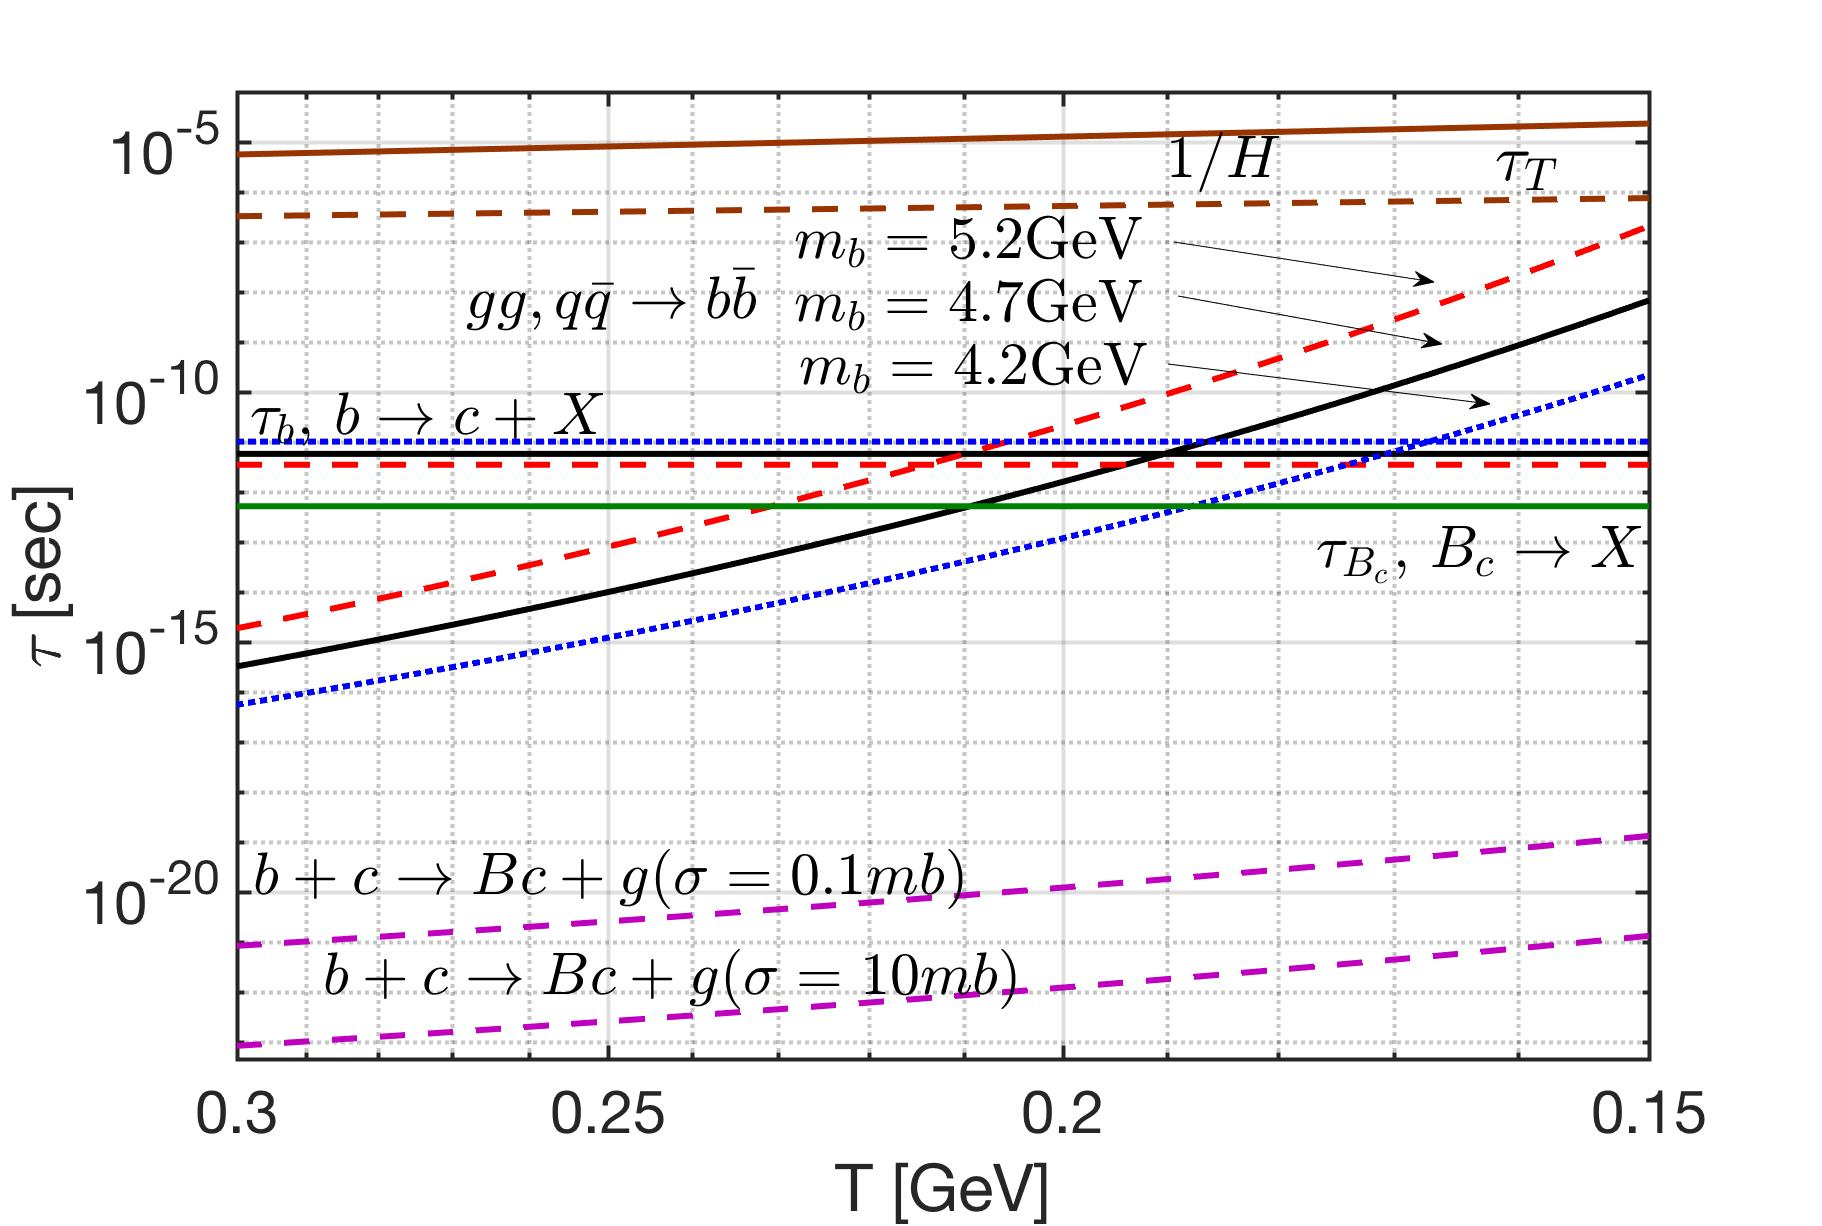
\includegraphics[width=0.9\linewidth]{./plots/BQuarkReactionTime003}}
\caption{Characteristic production, decay, times of bottom quark as a function of temperature $T$ for $0.3\,\mathrm{GeV}>T> 0.15\MeV$. Near the top of figure $1/H$ (brown solid line) and $\tau_T$ (brown dashed line); other horizontal lines are bottom-quark (in QGP) weak interaction lifetimes $\tau_b$ for the three different masses: $m_b=4.2\,\mathrm{GeV}$ (blue dotted line), $m_b=4.7\,\mathrm{GeV}$ (black solid line), $m_b=5.2\,\mathrm{GeV}$ (red dashed line), and the vacuum lifespan $\tau_B$ of the B$_c$ meson (green solid line). The relaxation time for strong interaction bottom production $g+g, q+\bar q\rightarrow b+\bar{b}$ is shown with three different bottom masses and same type-color coding as weak interaction decay rate. At bottom of figure the in plasma formation process (dashed lines, purple) $b+c\rightarrow \mathrm{B}_c+g$ with cross section range $\sigma=0.1,10\,\mathrm{mb}$. \radapt{Yang:2024ret}}
\label{ReactionTime}
\end{figure}
%%%%%%%%%%%%%%%%%%%%%%%%%%%%%%%%%

Considering all bottom flavor is free in QGP, the bottom decay rate per volume is the bottom lifespan weighted with density of particles \req{BoltzN}, see Ref.\,\cite{Kuznetsova:2008jt}. We have
\begin{align}\hspace{0.5cm}
R^{\mathrm{Decay}}_b=\frac{dn_b/d\Upsilon_b}{\tau_b},\,\,\,\,\, \tau_b\approx0.57\times10^{-11} \mathrm{sec}.
\end{align}
On the other hand, $b$,\,$\bar b$ quark abundance is embedded in a large background comprising all lighter quarks and antiquarks (see~\rf{number_entropy_b002}). After formation the heavy $b,\,\bar b$ quark can bind with any of the available lighter quarks, with the most likely outcome being a chain of reactions 
\begin{align}
&b+q\longrightarrow\mathrm{B}+g\;,\\
&\mathrm{B}+s\longrightarrow\mathrm{B}_s+q\;,\\
&\mathrm{B}_s+c\longrightarrow\mathrm{B}_c+s\;,
\end{align}
with each step providing a gain in binding energy and reduced speed due to the diminishing abundance of heavier quarks $s, c$. To capture the lower limit of the rate of $\mathrm{B}_c$ production we show in~\rf{ReactionTime} the expected formation rate by considering the direct process $b+\overline c\rightarrow \mathrm{B}_c+g$, considering the range of cross section $\sigma=0.1\sim10\,\mathrm{mb}$ ~\cite{Schroedter:2000ek}. The rapid formation rate of B$_c(b\bar c)$ states in primordial plasma is shown by purple dashed lines at bottom in~\rf{ReactionTime}, we have
\begin{align}
\tau (b+\overline c\rightarrow \mathrm{B}_c+g)\approx(10^{-16}\sim10^{-14})\times\frac{1}{H} \;.
\end{align}

Despite the low abundance of charm, the rate of $\mathrm{B}_c$ formation is relatively fast, and that of lighter flavored B-mesons is substantially higher. Note that as long as we have bottom quarks made in gluon/quark fusion bound practically immediately with any quarks $u, d, s$ into B-mesons, we can use the production rate of $b, \bar b$ pairs as the rate of B-meson formation in the primordial-QGP, which all decay with lifespan of pico-seconds. We believe that this process is fast enough to allow consideration of bottom decay from the B$_c(b\bar c)$, $\overline{\mathrm{B}}_c(\bar b c)$ states~\cite{Yang:2020nne}. 
 
Based on the hypothesis that all bottom flavor is bound rapidly into $\mathrm{B}_c^\pm$ mesons, we have 
\begin{align}\label{Bc_source}
g+g, q+q \longleftrightarrow &b+\bar b\;[b(\bar{b})+\bar{c}(c)]\longrightarrow \mathrm{B}_c^\pm\longrightarrow\mathrm{anything}.
\end{align}
In this case, the decay rate per volume can be written as
\begin{align}\hspace{0.5cm}
 R^{\mathrm{Decay}}_b=\frac{dn_b/d\Upsilon_b}{\tau_{\mathrm{B}_c}},\,\,\,\,\, \tau_{\mathrm{B}_c}\approx0.51\times10^{-12} \mathrm{sec}.
 \end{align}


%%%%%%%%%%%%%%%%%%%%%%%%%%%%%%%
\para{Stationary and non-stationary deviation from equilibrium}
To investigate the nonequilibrium phenomena of bottom quarks, we aim to replace the variation of particle abundance seen on LHS in \req{Bquark_eq} by the time variation of abundance fugacity $\Upsilon$.
This substitution allows us to derive the dynamic equation for the fugacity parameter and enables us to study the fugacity as a function of time. Considering the expansion of the Universe we have
\begin{align}\label{number_dilution}
\frac{1}{V}\frac{dN_b}{dt}=\frac{dn_b}{d\Upsilon_b}\frac{d\Upsilon_b}{dt}+\frac{dn_b}{dT}\frac{dT}{dt}+3Hn_b,\;
\end{align}
where we use $d\ln(V)/dt=3H$ for the Universe expansion. Substituting \req{number_dilution} into \req{Bquark_eq} and dividing both sides of equation by $dn_b/{d\Upsilon_b}=n^{th}_b$, the fugacity equation becomes
\begin{align}
\frac{d\Upsilon_b}{dt}+&3H\Upsilon_b+\Upsilon_b\frac{dn^{th}_b/dT}{n^{th}_b}\frac{dT}{dt}=\left(1-\Upsilon_b^2\right)\frac{1}{\tau_{b}^{\mathrm{Source}}}-\Upsilon_b\frac{1}{\tau^{\mathrm{Decay}}_b}\;,
\end{align}
where relaxation time for bottom production is obtained using \req{relaxation_time}. It is convenient to introduce the relaxation time $1/\tau_T$ as follows,
\begin{align}
\frac{1}{\tau_T}\equiv-\frac{dn^{th}_b/dT}{n^{th}_b}\frac{dT}{dt},
\end{align}
where we put '$-$' sign in the definition to have $\tau_T>0$. The relaxation time $\tau_T$ represents how the bottom density changes due to the Universe temperature cooling. In this case, the fugacity equation can be written as
\begin{align}\label{Fugacity_Eq0}
\frac{d\Upsilon_b}{dt}\!\!=&(1-\Upsilon_{b}^2)\frac{1}{\tau_{b}^{\mathrm{Source}}}
\!-\!\Upsilon_{b}\left(\frac{1}{\tau^{\mathrm{Decay}}_b}+3H\!-\!\frac{1}{\tau_T}\right).
\end{align}
In following sections we will solve the fugacity differential equation in two different scenarios: stationary and non-stationary Universe.

%%%%%%%%%%%%%%%%%%%%%%%%%%%%%%%%%%%%%%%%%%%
In~\rf{BCreaction:fig} (bottom) we show that the relaxation time for both production and decay are faster than the Hubble time $1/H$ for the duration of QGP, which implies that $H,1/\tau_T\ll1/\tau_{b}^{\mathrm{Source}},1/\tau^{\mathrm{Decay}}_b$. In this scenario, we can solve the fugacity equation by considering the stationary Universe first, i.e., the Universe is not expanding and we have
\begin{align}\label{stationary}
H=0,\qquad 1/\tau_T=0.
\end{align} 
In the stationary Universe at each given temperature we consider the dynamic equilibrium condition (detailed balance) between production and decay reactions that keep
\begin{align}
\frac{d\Upsilon_b}{dt}=0.
\end{align}
Neglecting the time dependence of the fugacity $d\Upsilon_b/dt$ and substituting the condition \req{stationary} into the fugacity equation \req{Fugacity_Eq0}, then we can solve the quadratic equation to obtain the stationary fugacity as follows: %\index{bottom quark!stationary fugacity}
\begin{align}
\label{Fugacity_Sol}
\Upsilon_{\mathrm{st}}&=\sqrt{1+\left(\frac{\tau_{source}}{2\tau_{decay}}\right)^2}-\left(\frac{\tau_{source}}{2\tau_{decay}}\right).
\end{align} 

%%%%%%%%%%%%%%%%%%%%%%%%%%%%%%%%%%%%%%
\begin{figure} 
\centerline{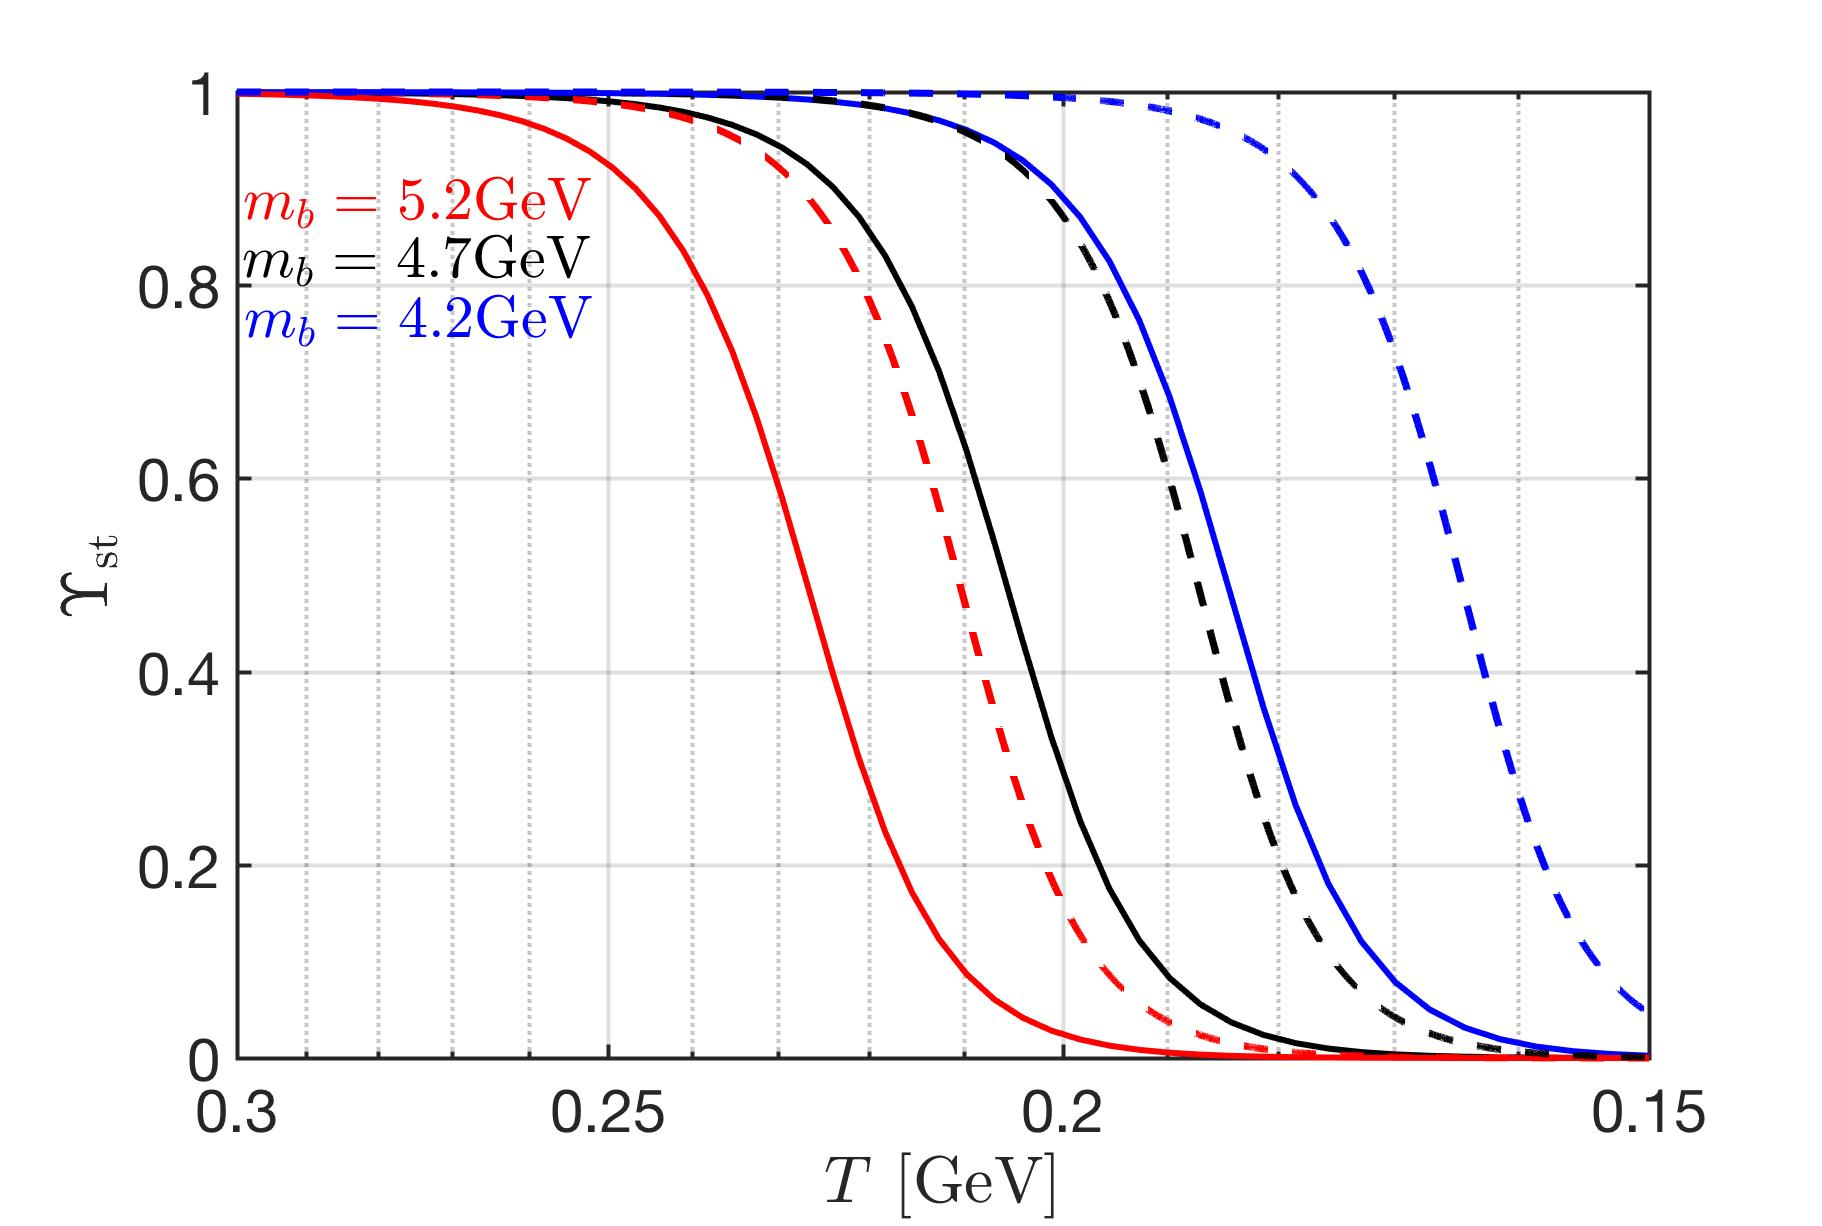
\includegraphics[width=0.9\linewidth]{./plots/BquarkFugacity_tot}}
\caption{Dynamical fugacity of bottom quark as a function of temperature in primordial Universe. Solid line shows bottom quark bound into $B_c$, dashed lines the case of free bottom quark: $m_b=4.2\,\mathrm{GeV}$ (blue), $m_b=4.7\,\mathrm{GeV}$ (black), and $m_b=5.2\,\mathrm{GeV}$ (red). \cccite{Rafelski:2023emw}. \radapt{Yang:2024ret}}
\label{fugacity_bc}
\end{figure}
%%%%%%%%%%%%%%%%%%%%%%%%%%%%%%%%%%%%%%%%%

In~\rf{fugacity_bc} the fugacity of bottom quark $\Upsilon_{\mathrm{st}}$ as a function of temperature, \req{Fugacity_Sol} is shown around the temperature $T=0.3\,\mathrm{GeV}>T>0.15\,\mathrm{GeV}$ for different masses of bottom quarks. In all cases we see prolonged nonequilibrium, this happens since the decay and reformation rates of bottom quarks are comparable to each other as we have noted in~\rf{ReactionTime} where both lines cross. One of the key results shown in~\rf{fugacity_bc} is that the smaller mass of bottom quark slows the strong interaction formation rate to the value of weak interaction decays just near the phase transformation of QGP to HG phase. Finally, the stationary fugacity corresponds to the reversible reactions in the stationary Universe. In this case, there is no arrow in time for bottom quark because of the detailed balance.

We now consider non-stationary correction in expanding Universe allowing for the Universe expanding and thus temperature being a function of time. This leads to non-stationary correction related to time dependent fugacity in the expanding Universe. 

In general, the fugacity of bottom quark can be written as 
\begin{align}\label{Nonstationary_sol}
&\Upsilon_b=\Upsilon_{\mathrm{st}}+\Upsilon^{\mathrm{non}}_{\mathrm{st}}=\Upsilon_\mathrm{st}\left(1+x\right),\quad x\equiv{\Upsilon_\mathrm{st}^{\mathrm{non}}}/{\Upsilon_\mathrm{st}},
\end{align}
where the variable $x$ corresponds to the correction due to non-stationary Universe. Substituting the general solution \req{Nonstationary_sol} into differential equation \req{Fugacity_Eq0}, we obtain
\begin{align}\label{Nonstationary_eq}
\frac{dx}{dt}=-x^2\frac{\Upsilon_\mathrm{st}}{\tau_{source}}&-x\left[\frac{1}{\tau_{eff}}+3H-\frac{1}{\tau_T}\right]-\left[\frac{d\ln\Upsilon_\mathrm{st}}{dt}+3H-\frac{1}{\tau_T}\right],
\end{align}
where the effective relaxation time $1/\tau_{eff}$ is defined as
\begin{align}
\frac{1}{\tau_{eff}}\equiv\left[\frac{2\Upsilon_\mathrm{st}}{\tau_{source}}+\frac{1}{\tau_{decay}}+\frac{d\ln\Upsilon_\mathrm{st}}{dt}\right].
\end{align}

%%%%%%%%%%%%%%%%%%%%%%%%%%%%%%
\begin{figure} 
\centerline{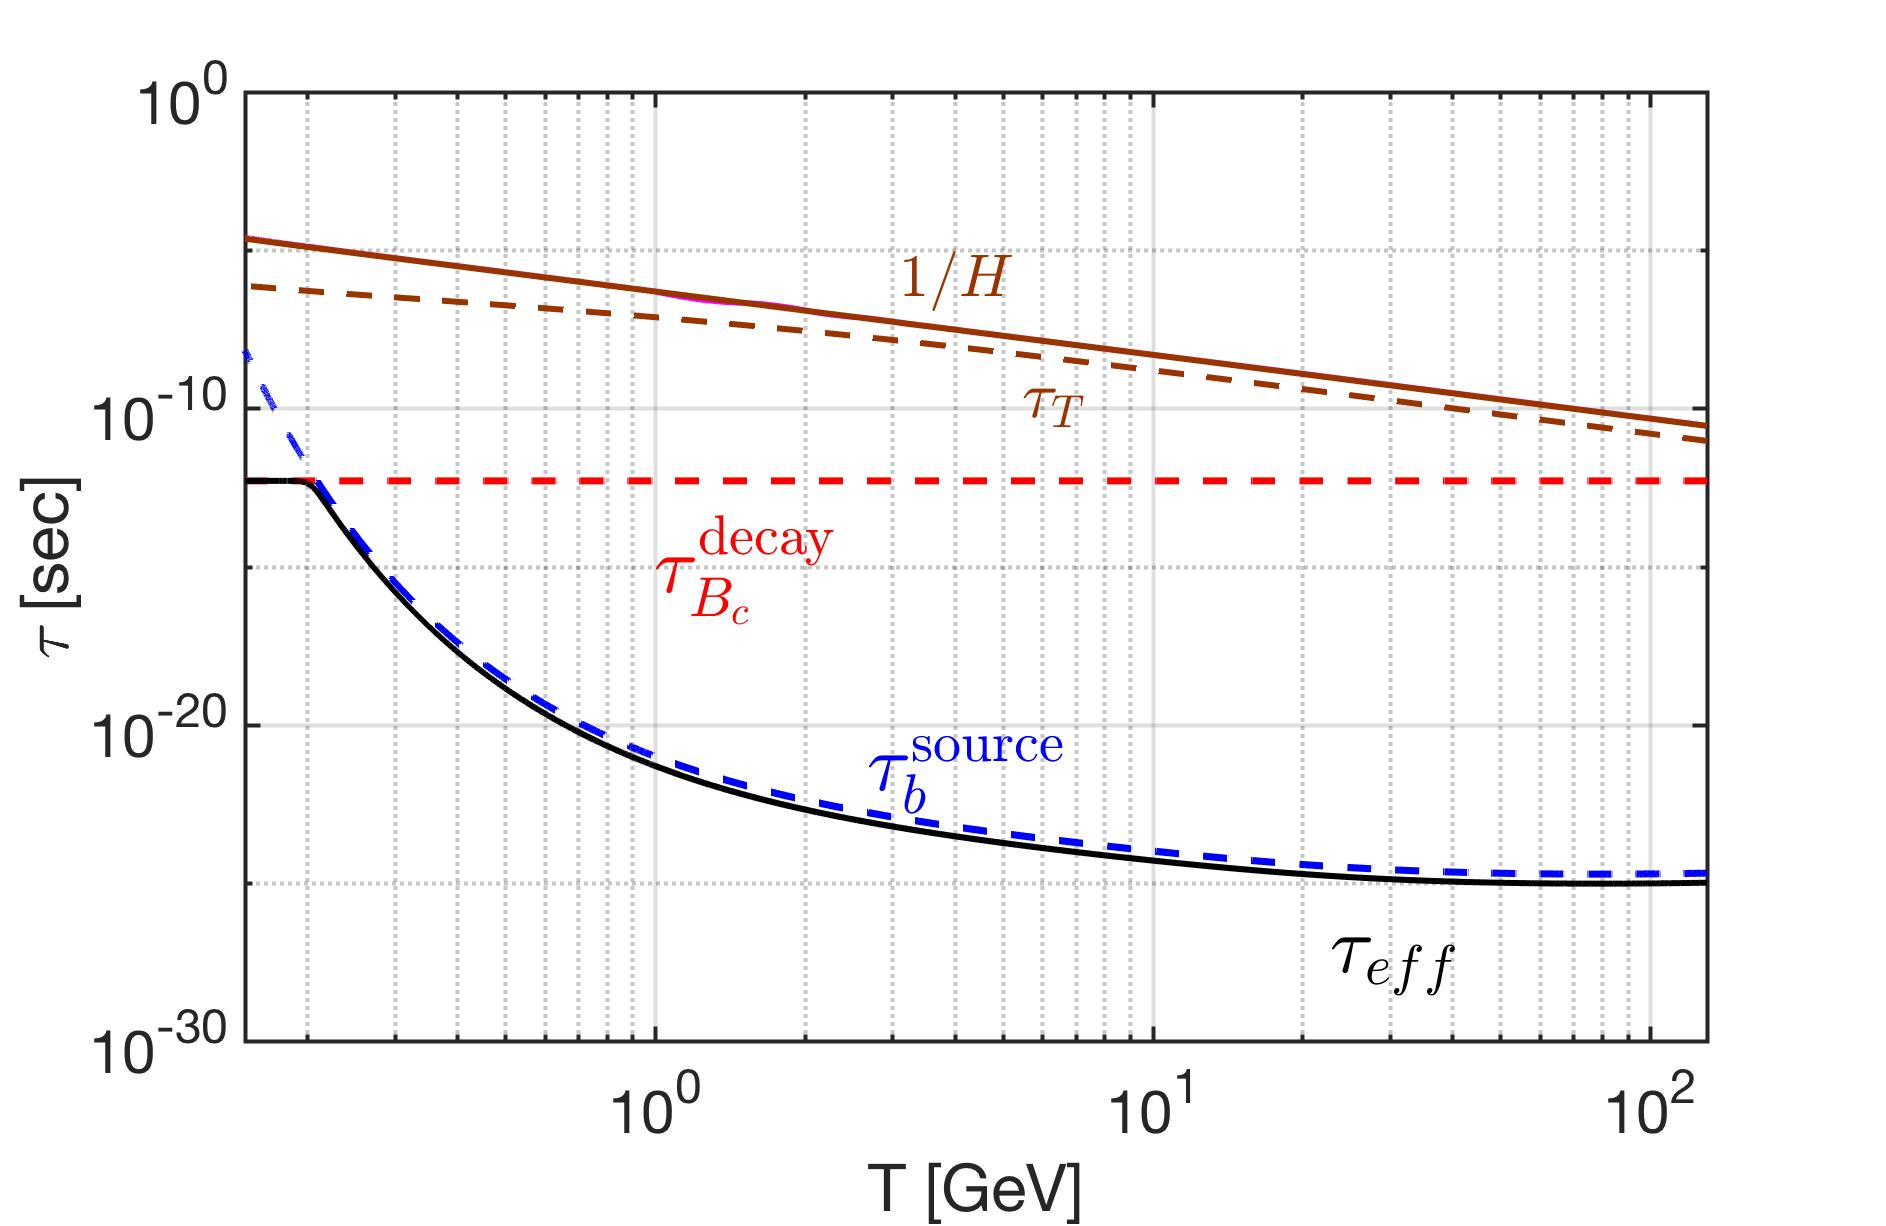
\includegraphics[width=0.9\linewidth]{./plots/Tau_RelaxationTime002}}
\caption{The effective relaxation time $\tau_{eff}$ as a function of temperature in the primordial Universe for bottom mass $m_b=4.7$\,GeV. For comparison, we also plot the vacuum lifespan of $B_c$ meson $\tau_{B_c}^{decay}$ (red dashed-line), the relaxation time for bottom production $\tau^b_{source}$ (blue dashed-line), Hubble expansion time $1/H$(brown solid line) and relaxation time for temperature cooling $\tau_T$ (brown dashed-line). \radapt{Yang:2024ret}}
\label{RelaxationTime_eff}
\end{figure}
%%%%%%%%%%%%%%%%%%%%%%%%%%%%%%%%%

In~\rf{RelaxationTime_eff} we see that when temperature is near to $T=0.2\GeV$, we have $1/\tau_{eff}\approx10^{7}H$, and $1/\tau_{eff}\approx10^5/\tau_T$. In this case, the last two terms in \req{Nonstationary_eq} compare to $1/\tau_{eff}$ can be neglected, and the differential equation becomes
\begin{align}\label{nonstationary_eq}
\frac{dx}{dt}=-\frac{x^2\,\Upsilon_\mathrm{st}}{\tau_{source}}&-\frac{x}{\tau_{eff}}-\left[\frac{d\ln\Upsilon_\mathrm{st}}{dt}+3H-\frac{1}{\tau_T}\right],
\end{align}

To solve the variable $x$ we consider the case $dx/dt,x^2\ll1$ first, we neglect the terms $dx/dt$ and $x^2$ in \req{nonstationary_eq} then solve the linear fugacity equation. We will establish that these approximations are justified by checking the magnitude of the solution. Neglecting terms $dx/dt$ and $x^2$ in \req{nonstationary_eq} we obtain
\begin{align}
x\approx\tau_{eff}\left[\frac{d\ln\Upsilon_\mathrm{st}}{dt}+3H-\frac{1}{\tau_T}\right].
\end{align}
It is convenient to change the variable from time to temperature. For an isentropically-expanding universe, we have
\begin{align}\label{tau_H}
\frac{dt}{dT}=-\frac{\tau^\ast_H}{T},\qquad \tau^\ast_H=\frac{1}{H}\left(1+\frac{T}{3g^s_\ast}\frac{dg^s_\ast}{dT}\right).
\end{align}
In this case, we have
\begin{align}
x=\tau_{eff}\left[\frac{1}{\Upsilon_\mathrm{st}}\frac{d\Upsilon_\mathrm{st}}{dT}\frac{T}{\tau^\ast_H}+3H-\frac{1}{\tau_T}\right].
\end{align}
Finally, we can obtain the non-stationary fugacity by multiplying the fugacity ratio $x$ with $\Upsilon_\mathrm{st}$, giving \index{bottom quark! non-stationary fugacity}
\begin{align}
\Upsilon_{\mathrm{st}}^{\mathrm{non}}
&\approx\left(\frac{\tau_{eff}}{\tau^\ast_H}\right)\left[\frac{d\Upsilon_\mathrm{st}}{dT}T-\Upsilon_{\mathrm{st}}\left(3H\tau^\ast_H-\frac{\tau^\ast_H}{\tau_T}\right)\right].
\end{align}

In~\rf{NonFugacity} we plot the non stationary $\Upsilon^{\mathrm{non}}_\mathrm{st}$ as a function of temperature. The non stationary fugacity $\Upsilon^{\mathrm{non}}_\mathrm{st}$ follows the behavior of $d\Upsilon_{\mathrm{st}}/dT$, which corresponds to the irreversible process in expanding Universe. In this case, the irreversible nonequilibrium process creates the arrow in time for bottom quark in the Universe. The large value of Hubble time compares to the effective relaxation time suppressing the value of non-stationary fugacity to $\mathcal{O}\sim10^{-7}$, which shows that the neglecting $dx/dt,x^2\ll1$ is a good approximation for solving the non-stationary fugacity in the primordial Universe.


%%%%%%%%%%%%%%%%%%%%%%%%%%%%%%%%%%%
\begin{figure}
\centerline{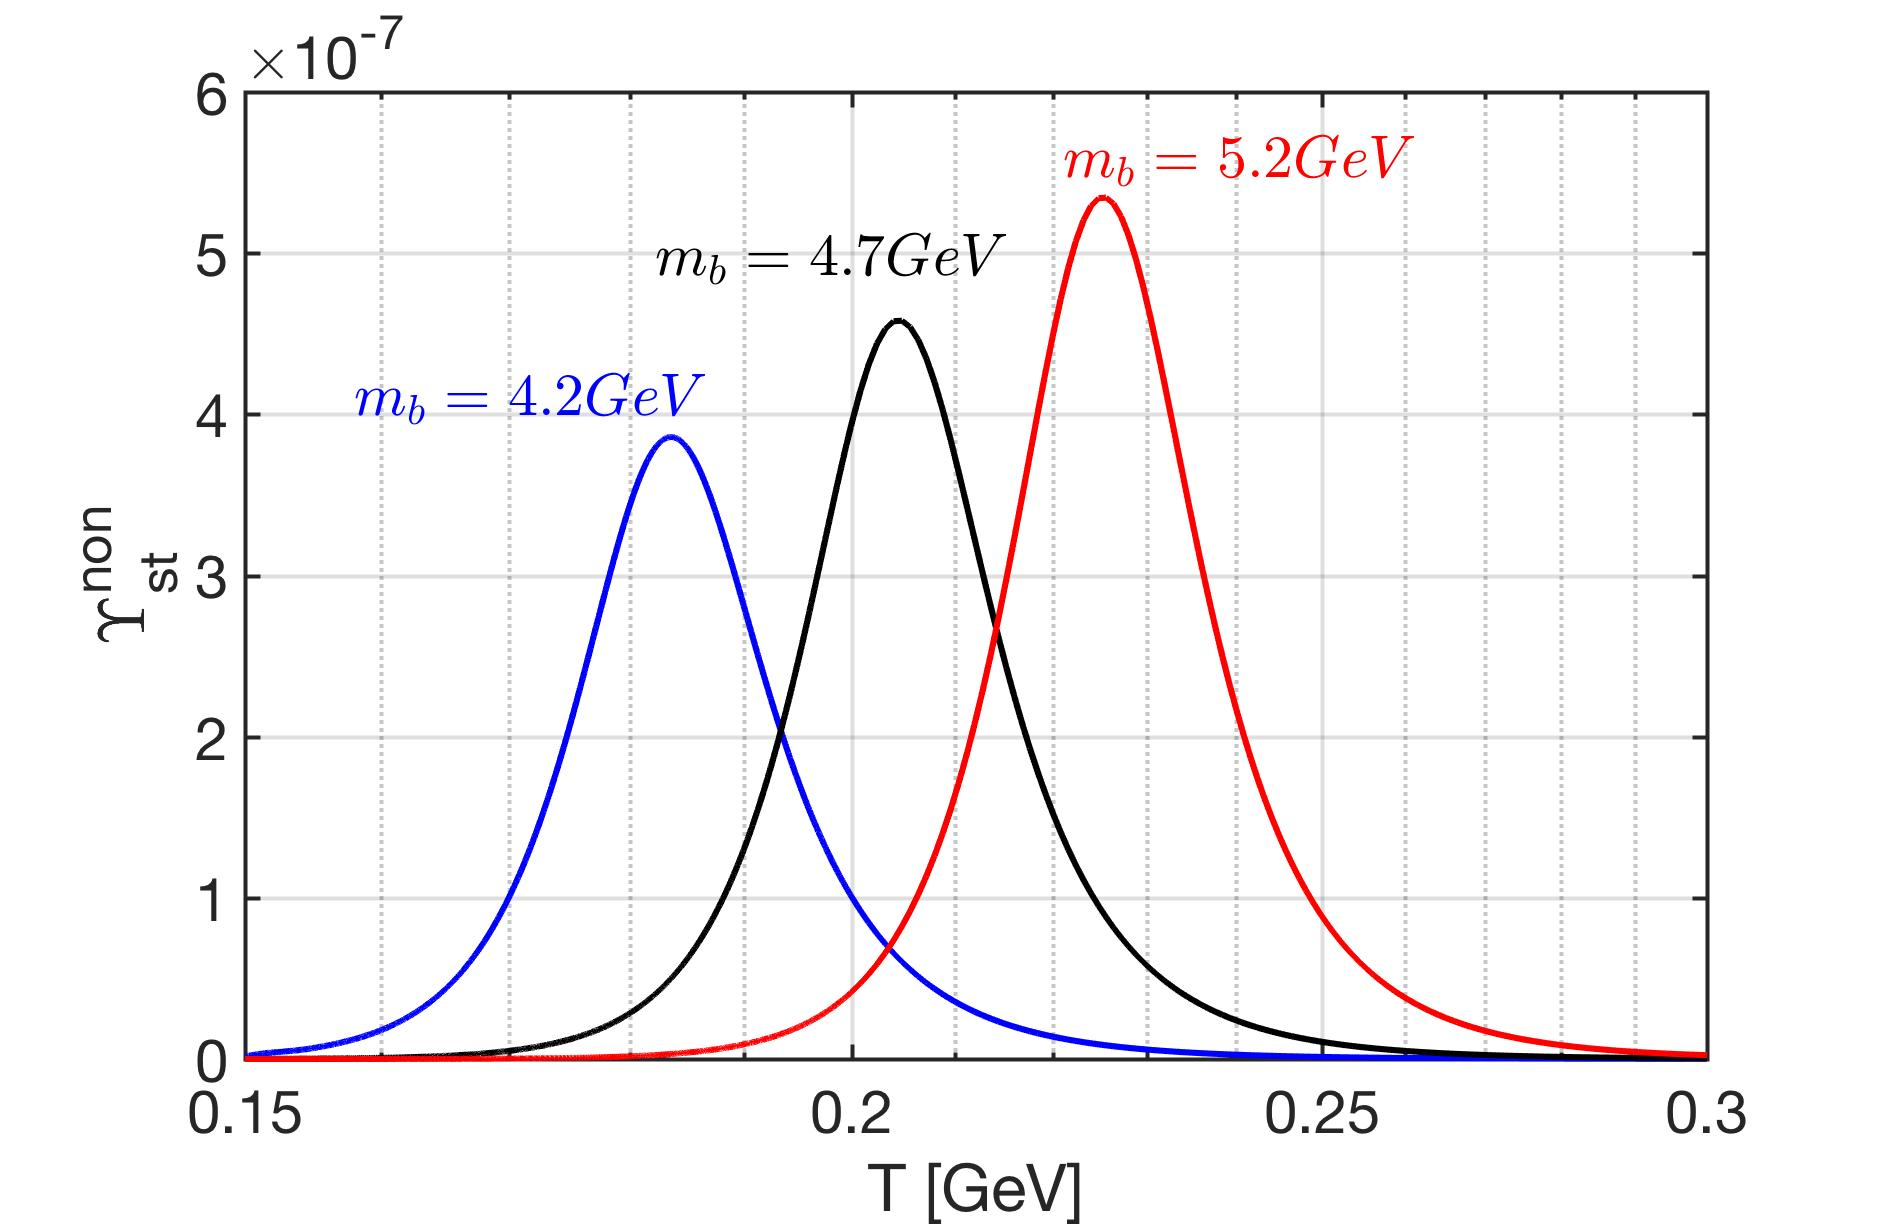
\includegraphics[width=0.9\linewidth]{./plots/NonstationaryFugacity}}
\caption{The non-stationary fugacity $\Upsilon_\mathrm{st}^{\mathrm{non}}$ as a function of temperature in the Universe for different bottom mass $m_b=4.2\,\mathrm{GeV}$ (blue), $m_b=4.7\,\mathrm{GeV}$ (black), and $m_b=5.2\,\mathrm{GeV}$ (red) for the case bottom quarks bound into $B_c$ mesons. \radapt{Yang:2024ret}}
\label{NonFugacity}
\end{figure}
%%%%%%%%%%%%%%%%%%%%%%%%%%%%%%%%%%%%%%
 

%%%%%%%%%%%%%%%%%%%%%%%%%%%%%%%%%%
\para{Is there enough bottom flavor to matter?} Considering that FLRW-Universe evolves conserving entropy, and that baryon and lepton number following on the era of matter genesis is conserved, the current day baryon $B$ to entropy $S$, $B/S$-ratio must be achieved during matter genesis. The estimates of present day baryon-to-photon density ratio $\eta$ allows the determination of the present value of baryon per entropy ratio \cite{Rafelski:2019twp,Letessier:2002ony,Fromerth:2002wb,Fromerth:2012fe}:
\begin{align}
\left(\frac{B}{S}\right)_{t_0}\!\!\!\!=\eta\left(\frac{n_\gamma}{\sigma_\gamma+\sigma_\nu}\right)_{\!t_0}\!\!\!\!=(8.69\pm0.05)\!\!\times\!\!10^{-11},
\end{align}
where the subscript $t_0$ denotes the present day value, where $\eta=(6.12\pm0.04)\times10^{-10}$~\cite{ParticleDataGroup:2018ovx} is used in calculation. Here we consider that the Universe today is dominated by photons and free-streaming low mass neutrinos~\cite{Birrell:2012gg}, and $\sigma_\gamma$ and $\sigma_\nu$ are the entropy density for photons and neutrinos, respectively. 
 
In chemical equilibrium the ratio of bottom quark (pair) density $n_b^{th}$ to entropy density $\sigma=S/V$ just above quark-gluon hadronization temperature $T_\mathrm{H}=150\sim160\MeV$ is $n_b^{th}/\sigma=10^{-10}\sim 10^{-13}$ (see~\rf{number_entropy_b002}. By studying the bottom density per entropy near to the hadronization temperature and comparing it to the baryon-per-entropy ratio $B/S$ we found that there is sufficient abundance of bottom quarks for the proposed matter genesis mechanism to be relevant.

%%%%%%%%%%%%%%%%%%%%%%%%%%%%%%%%
\para{Example of bottom-catalyzed matter genesis}
Given that the nonequilibrium non-stationary component of bottom flavor arises at relatively low QGP temperature, this Sakharov condition is available around QGP hadronization. Let us now look back and see how different requirements are fulfilled
%%%%%%%%%%%%%%%%%%%%%%%%%%%%%%%%%%%%
\begin{itemize}
\item
 We have demonstrated non-stationary conditions with absence of detailed balance: The competition between weak interaction decay and the strong interaction gluon fusion process is responsible for driving the bottom quark departure from the equilibrium in the primordial Universe near to QGP hadronization condition around the temperature $T=0.3\sim0.15\GeV$ as shown in~\rf{fugacity_bc}. Albeit small there is clear non-stationary component required for baryogenesis, see~\rf{NonFugacity}.
%%%%%%%%%%%%%%%%%%%%%%%%%%%%%%%
\item Violation of $CP$ asymmetry were observed in the amplitudes of hadron decay including neutral B-mesons, see for example~\cite{LHCb:2019jta,LHCb:2020vut}. The weak interaction $CP$ violation\index{CP!violation}\index{CKM!mtrix} arises from the components of Cabibbo-Kobayashi-Maskawa (CKM) matrix associated with quark-level transition amplitude and $CP$-violating phase. There is clear coincidence of non stationary component of bottom yield with the bottom quark $CP$ violating decays of preformed $\mathrm{B}_x$ meson states, $x=u,d,s,c$~\cite{Karsch:1987pv,Brambilla:2010vq,Aarts:2011sm,Brambilla:2017zei,Bazavov:2018wmo,Offler:2019eij}. The exploration of the here interesting $CP$ symmetry breaking in B$_c(b\bar c)$ decay is in progress~\cite{Tully:2019ltb,HFLAV:2019otj,ParticleDataGroup:2018ovx}. % Present measurements of $CP$-violation suggest that the CP asymmetry parameter is around $\delta_{CP}\approx10^{-3}$ ~\cite{ParticleDataGroup:2018ovx}.
\item
We do not know if there is baryon number violating process in which one of the heavy particles, including bottom quark, is participating. However, if such a process were to exist it is likely, considering mass thresholds, that it would be most active in the decays of heaviest standard model particles. It is thus of considerable interest to study in lepton colliders baryon number non conserving processes at resonance condition. Such a research program will additionally be motivated by our demonstration of an extended period of baryogenesis in the primordial Universe. 
\end{itemize}

%%%%%%%%%%%%%%%%%%%%


\para{Circular Urca amplification}
The off equilibrium phenomenon of bottom quark around the temperature range $T=0.3\sim0.15\GeV$ can provide the non-chemical equilibrium non-stationary condition for baryogenesis to occur in the primordial-QGP hadronization era. The processes of interest as we saw are small. However there is additional amplifying factor. 
 
 Let us consider the scenario where all bottom quarks are confined within $B_c^\pm$ meson. In this case, the decay of charged mesons in the primordial-QGP can be a source of $CP$ violation. However, it remains uncertain whether the decay of $B_c^\pm$ mesons contributes to baryon violation. Our postulation is as follows: the baryon asymmetry is produced by the bottom quark disappearance via the irreversible decay of $B^\pm_c$ meson during the off-equilibrium process. Once a baryon symmetry exists in universe, it will also produce the asymmetry between leptons and anti-leptons which is similar to the baryon asymmetry by the $L=B$.

The heavy $B_c^\pm$ meson decay into multi-particles in plasma is associated with the irreversible process. This is because after decay the daughter particles can interact with plasma and distribute their energy to other particles and reach equilibrium with the plasma quickly. In this case the energy required for the inverse reaction to produce $B_c^\pm$ meson is difficult to overcome and therefore we have an irreversible process for multi-particle decay in plasma.


The rapid $B_c^\pm$ decay and bottom reformation speed at picosecond scale assures that there are millions of individual microscopic processes involving bottom quark production and decay before and during the hadronization epoch of QGP. In this case, we have an Urca process for the bottom quark, i.e. a cycling reaction that produces the bottom quark which subsequently disappears via the $B_c^\pm$ meson decay. 

The Urca process is a fundamental physical process and has been studying the realms of in astrophysics and nuclear physics. In our case, for bottom quark as a example: at low temperature, the number of bottom quark cycling can be estimated as
\begin{align}
\left.\mathrm{C_{cycle}}\right|_{T=0.2\mathrm{GeV}}=\frac{\tau_H}{\tau_{B_c}}\approx2\times10^7,
\end{align}
where the lifespan of $B_c^\pm$ is $\tau_{\mathrm{B}_c}\approx0.51\times10^{-12}\,\mathrm{sec}$ and at temperature $T=0.2\GeV$ the Hubble time is $\tau_H=1/H=1.272\times10^{-5}$ sec. The Urca process plays a significant role by potentially amplifying any small and currently unobserved violation of baryon number associated with the bottom quark. The small baryon asymmetry is enhanced by the Urca-like process with cycling ${\tau^\ast_H}/{\tau_\ast}$ in the primordial Universe.
This amplification would be crucial for achieving the required strength for today's observation. 


%%%%%%%%%%%%%%%%%%%%%%%%%%%%%%%%%%%%%%%%%%%%%%%%
\subsection{Strange hadron abundance in cosmic plasma}
\label{Strangeness}\index{strangeness}
%%%%%%%%%%%%%%%%%%%%%%%%%%%%%%%%%%
\para{Hadron populations in equilibrium}
As the Universe expanded and cooled down to the QGP Hagedorn temperature $T_H\approx150\MeV$, the primordial QGP underwent a phase transformation called hadronization. Quarks and gluons fragmented, combined and formed matter and antimatter  we are familiar with. After hadronization, one may think that all relatively short lived massive hadrons decay rapidly and disappear from the Universe. However, the most abundant hadrons, pions $\pi(q\bar q)$, can be produced via their inverse decay process $\gamma\gamma\rightarrow\pi^0$. Therefore they retain their chemical equilibrium  down to $T=3\sim5\MeV$~\cite{Kuznetsova:2008jt}. 

We begin by determining the Universe particle population composition assuming both kinetic and particle abundance equilibrium (chemical equilibrium) of non-interacting bosons and fermions. By considering the charge neutrality and a prescribed conserved baryon-per-entropy-ratio ${(n_B-n_{\overline{B}})}/{\sigma}$ we can  determine the baryon chemical potential $\mu_B$~\cite{Fromerth:2002wb,Fromerth:2012fe,Rafelski:2013yka}. We extend this approach  allowing for the presence of strange hadrons, and imposing conservation of strangeness in the primordial Universe -- the  strange quark content in hadrons must equal the anti-strange quark content in statistical average $\langle s-\bar s \rangle=0$. 

Given $\mu_B(T)$, $\mu_s(T)$ the baryon and strangeness chemical potentials as a function of temperature, we can obtain the particle number densities for different strange and non-strange species and study their population in the primordial Universe. Our approach prioritizes strangness pair production into bound hadron states by strong or electromagnetic interactions over the also possible weak interaction strangness changing processes capable to amplify the effect of baryon asymmetry. This is another topic beyond scope of this work and deserving further attention.

To characterize the baryon and strangeness content of a hadron we employ the chemical fugacity for strangeness $\lambda_s$ and for light quarks $\lambda_q$ \index{quark!fugacity}
\begin{align}
\lambda_s=\exp(\mu_s/T)\,\quad \lambda_q=\exp(\mu_B/3T)\,.
\end{align}
Here $\mu_s$ and $\mu_B$ are the chemical potential of strangeness and baryon, respectively. To obtain quark fugacity $\lambda_q$, we divide the baryo-chemical potential of baryons by quark content in the baryon, \ie\ three.

When the baryon chemical potential does not vanish the chemical potential of strangeness in the primordial Universe is obtained imposing the conservation of strangeness constraint $\langle s-\bar s \rangle=0$, see Section 11.5 in Ref.\,\cite{Letessier:2002ony}\index{strangeness! chemical potential}
\begin{align}\label{museq}
\lambda_s=\lambda_q\sqrt{\frac{F_K+\lambda^{-3}_q\,F_Y}{F_K+\lambda^3_q\,F_Y}}\,.
\end{align}
where we employ the phase-space function $F_i$ for sets of nucleon $N$, kaons $K$, and hyperon $Y$ particles 
\begin{align}
&F_N=\sum_{N_i}\,g_{N_i}W(m_{N_i}/T)\;, \quad N_i=n, p, \Delta(1232),\\
&F_K=\sum_{K_i}\,g_{K_i}W(m_{K_i}/T)\;, \quad K_i=K^0, \overline{K^0}, K^\pm, K^\ast(892),\\
&F_Y=\sum_{Y_i}\,g_{Y_i}W(m_{Y_i}/T)\;, \quad Y_i=\Lambda, \Sigma^0,\Sigma^\pm, \Sigma(1385),
\end{align}
$g_{N_i,K_i,Y_i}$ are the degeneracy factors, $W(x)=x^2K_2(x)$ with $K_2$ is the modified Bessel functions of integer order `$2$'. 

Considering the massive particle number density in the Boltzmann approximation we obtain
\begin{align}
\label{Density_N}
&n_N=\frac{T^3}{2\pi^2}\lambda_q^3F_N,\quad\qquad\qquad n_{\overline N}=\frac{T^3}{2\pi^2}\lambda^{-3}_qF_N,\\
\label{Density_K}
&n_K=\frac{T^3}{2\pi^2}\left(\lambda_s\lambda_q^{-1}\right)F_K,\,\qquad n_{\overline{K}}=\frac{T^3}{2\pi^2}\left(\lambda_s^{-1}\lambda_q\right)F_K,\\
\label{Density_Y}
&n_Y=\frac{T^3}{2\pi^2}\left(\lambda_q^2\lambda_s\right)F_Y,\quad\qquad n_{\overline Y}=\frac{T^3}{2\pi^2}\left(\lambda^{-2}_q\lambda_s^{-1}\right)F_Y.
\end{align}
In this case, the net baryon density in the primordial Universe with temperature range $150\MeV> T>10\MeV$ can be written as 
\begin{align}
\frac{\left(n_B-n_{\overline{B}}\right)}{\sigma}&=\frac{1}{\sigma}\left[\left(n_p-n_{\overline{p}}\right)+\left(n_n-n_{\overline{n}}\right)+\left(n_Y-n_{\overline{Y}}\right)\right]\notag\\
&=\frac{T^3}{2\pi^2\,\sigma}\left[\left(\lambda_q^3-\lambda^{-3}_q\right)F_N+\left(\lambda_q^2\lambda_s-\lambda^{-2}_q\lambda_s^{-1}\right)F_Y\right]\notag\\
&=\frac{T^3}{2\pi^2\sigma}\left(\lambda_q^3-\lambda_q^{-3}\right)F_N\left[1+\frac{\lambda_s}{\lambda_q}\left(\frac{\lambda_q^3-\lambda^{-1}_q\lambda_s^{-2}}{\lambda^3_q-\lambda^{-3}_q}\right)\,\frac{F_Y}{F_N}\right]\notag\\
&\approx\frac{T^3}{2\pi^2\sigma}\left(\lambda_q^3-\lambda_q^{-3}\right)F_N\left[1+\frac{\lambda_s}{\lambda_q}\,\frac{F_Y}{F_N}\right],
\end{align}
where we can neglect the term $F_Y/F_K$ in the expansion of \req{museq} in our temperature range. 

Introducing the strangeness conservation $\langle s-\bar s\rangle=0$ constraint and using the entropy density in primordial Universe, the explicit relation for baryon to entropy ratio becomes
\begin{align}\label{muBeq}
\frac{n_B-n_{\overline{B}}}{\sigma}&=\frac{45}{2\pi^4g^s_\ast}\sinh\left[\frac{\mu_B}{T}\right]F_N\times\left[1+\frac{F_Y}{F_N}\sqrt{\frac{1+e^{-\mu_B/T}\,F_Y/F_K}{1+e^{\mu_B/T}\,F_Y/F_K}}\right].
\end{align}
The present-day baryon-per-entropy-ratio is needed  in \req{muBeq}  and we obtain the value 
\begin{align}\label{BdS}
\frac{n_B-n_{\overline{B}}}{\sigma}= \left.\frac{n_B-n_{\overline{B}}}{ \sigma}\right|_{t_0}=(0.865\pm0.008)\times10^{-10} \;.
\end{align}

For a details of evaluation method we refer to our earlier work, however we have updated results to the updated baryon-to-photon ratio~\cite{ParticleDataGroup:2018ovx}: $\left(n_B-n_{\overline{B}}\right)/n_\gamma= (0.609\pm0.06)\times10^{-9}$, supplemented by quantum value of entropy per particle for a massless boson $\sigma/n|_\mathrm{boson}\approx 3.60$, and for a massless fermion $\sigma/n|_\mathrm{fermion}\approx 4.20$. We solve \req{museq}) and \req{muBeq} numerically to obtain baryon and strangeness chemical potentials as a function of temperature shown in~\rf{ChemPotFig}.

%%%%%%%%%%%%%%%%%%%%%%%%
\begin{figure} 
\centerline{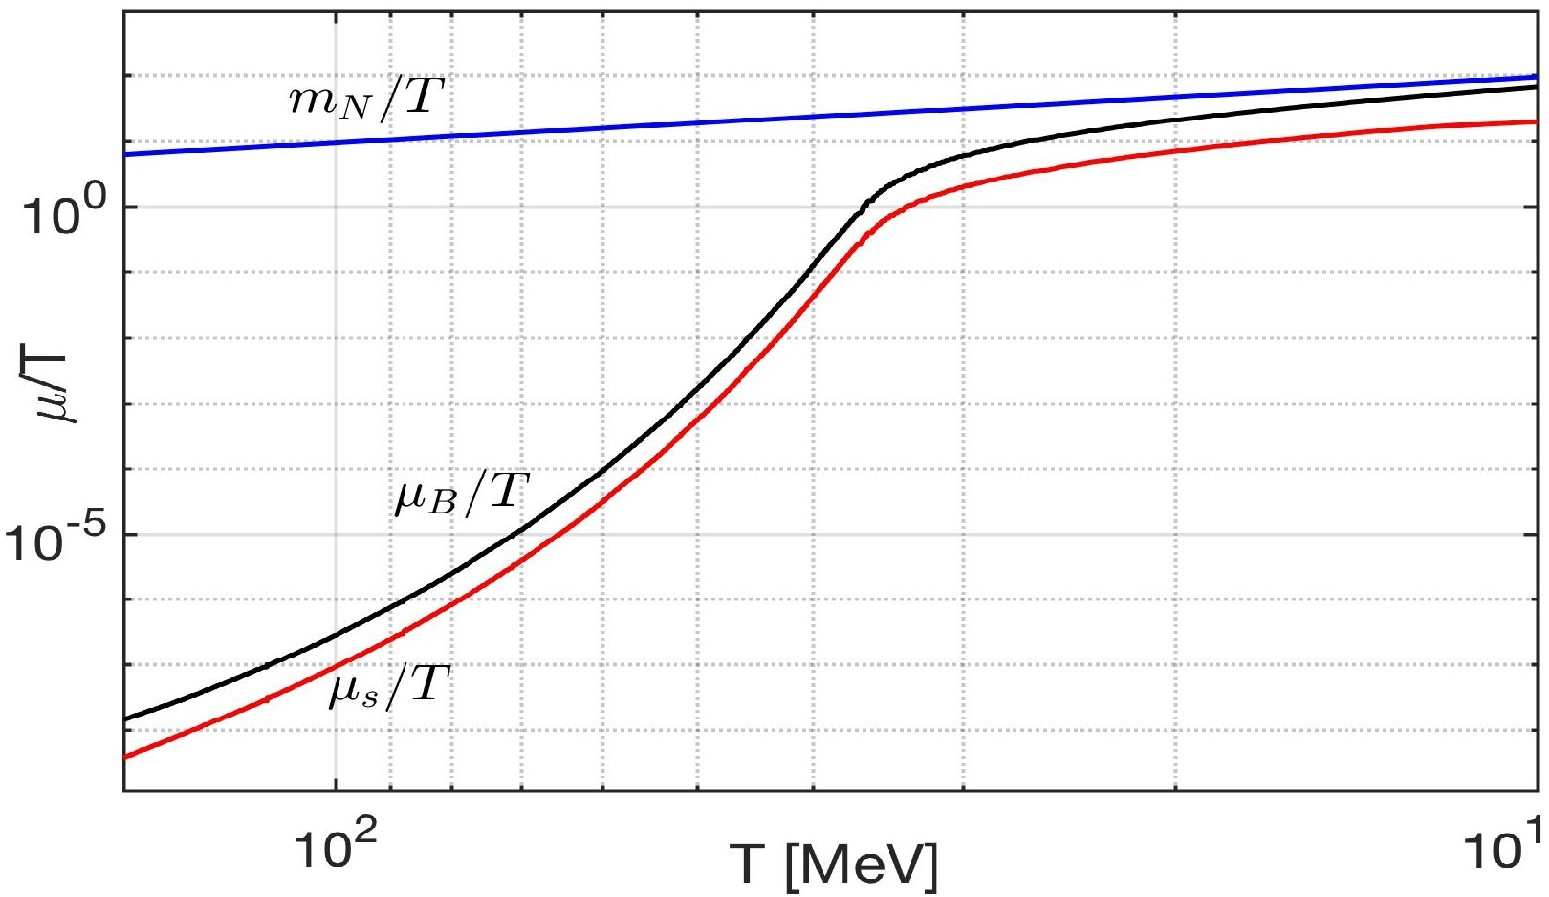
\includegraphics[width=0.9\linewidth]{./plots/New_Chemical_Potential_C.jpg}}
\caption{The chemical potential of baryon number $\mu_B/T$ and strangeness $\mu_s/T$ as a function of temperature $150\MeV> T>10\MeV$ in the primordial Universe; for comparison we show $m_N/T $ with $m_N=938.92\MeV$, the average nucleon mass. \cccite{Yang:2021bko}. \radapt{Yang:2024ret}}
\label{ChemPotFig}\index{baryon!chemical potential}\index{strangeness!chemical potential} 
\end{figure}
%%%%%%%%%%%%%%%%%%%%%%%%%%%%%%

The chemical potential in~\rf{ChemPotFig} changes dramatically in the temperature window $50\MeV\le T\le 30\MeV$, its behavior is describing the antibaryon disappearance from Universe inventory. Substituting the chemical potential $\lambda_q$ and $\lambda_s$ into particle density \req{Density_N}, \req{Density_K}, and \req{Density_Y}, we can obtain the particle number densities for different species as a function of temperature.

%%%%%%%%%%%%%%%%%%%%%%%%%%%%%%%%%%%%%%%
\begin{figure} 
\centerline{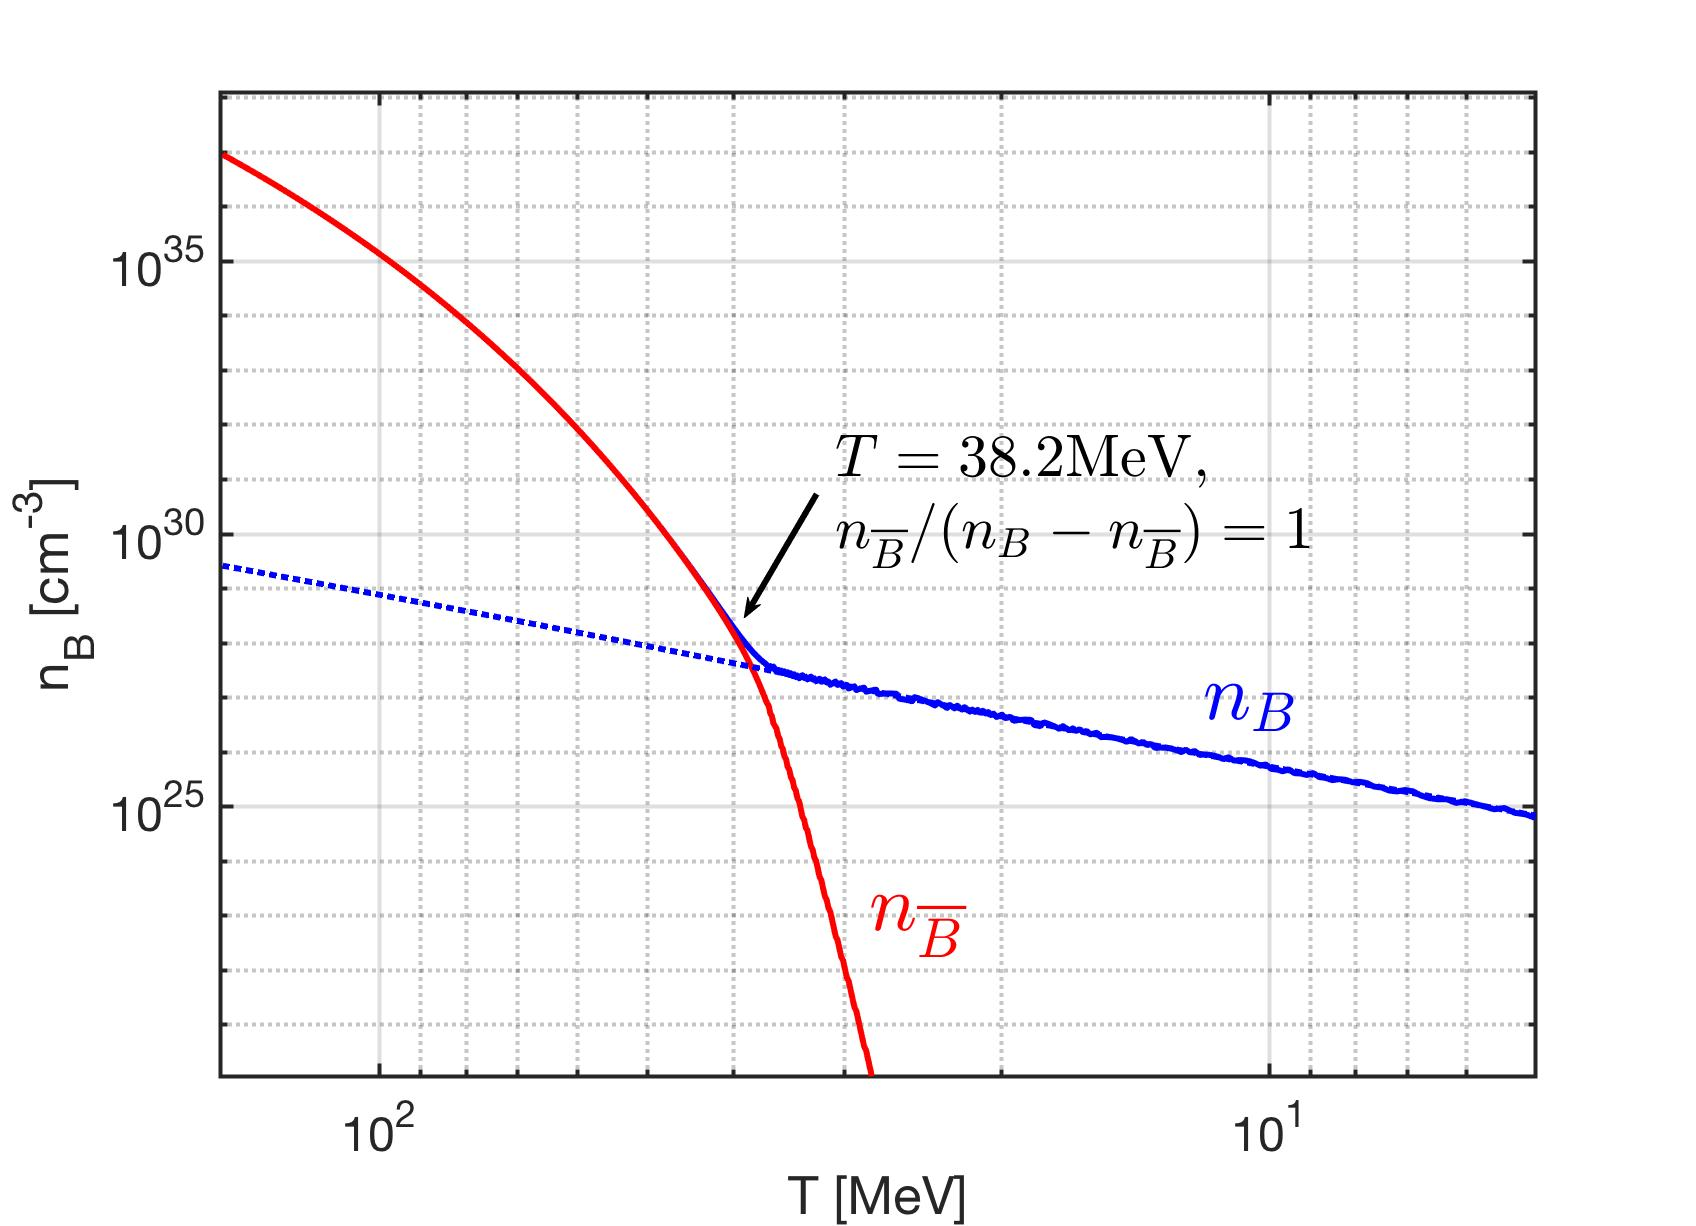
\includegraphics[width=0.9\linewidth]{./plots/Baryon_Antibaryon_cm.jpg}}
\caption{The antibaryon $n_{\overline  B}$ (red solid line) number density as a function of temperature in the range $150\MeV>T>5\MeV$. The blue solid line for baryons  $n_{B}$ merges into the antibaryon yield so that net baryon number $n_{B}-n_{\overline r B}$ (dashed blue line) continues the net  baryon yield seen as solid blue line. At temperature $T=38.2\MeV$  we have $n_{\overline B}/(n_B-n_{\overline B})=1$, antibaryons disappear from the Universe. \cccite{Rafelski:2023emw}. \radapt{Yang:2024ret}}
\label{Baryon:fig}\index{antibaryon!yield}
\end{figure}
%%%%%%%%%%%%%%%%%%%%%%%%%%%%%%%%%%%%%%%

In~\rf{Baryon:fig} we plot the number density of antibaryons (red line),  baryons (solid blue) and net baryon $n_B-n_{\overline B}$ (dashed blue) as a function of temperature. We determine the value of temperature $T=38.2\MeV$ to correspond to the condition $n_{\overline B}\ll(n_B-n_{\overline B})=1$, the effective antibaryon  disappearance temperature from the Universe inventory   $T=38.2\MeV$ is in agreement with the qualitative result presented in 1990 by Kolb and Turner~\cite{Kolb:1990vq}. Below this temperature, there antibaryons rapidly disappear, the net baryon density is the baryon asymmetry which dilutes keeping baryon to entropy ratio constant.

In~\rf{EquilibPartRatiosFig} we show examples of particle abundance ratios of interest\index{hadron!ratios}.   Pions $\pi(q\bar q)$ are the most abundant hadrons $n_\pi/n_B\gg1$, because of their low mass and the reaction $\gamma\gamma\rightarrow\pi^0$, which assures chemical yield equilibrium~\cite{Kuznetsova:2008jt} in the era of interest here. For $150\MeV>T>20.8\MeV$, we see the ratio $n_{{\overline K}(\bar q s)}/n_B\gg1$, which implies pair abundance of strangeness is more abundant than baryons, and is dominantly present in mesons, since $n_{\overline K}/n_Y\gg1$.  Considering $n_Y/n_B$ we see that hyperons $Y(sqq)$ remain a noticeable 1\% component in the baryon yield through the domain of antibaryon decoupling.

%%%%%%%%%%%%%%%%%%%%%%%%%%%%
\begin{figure} 
\centerline{
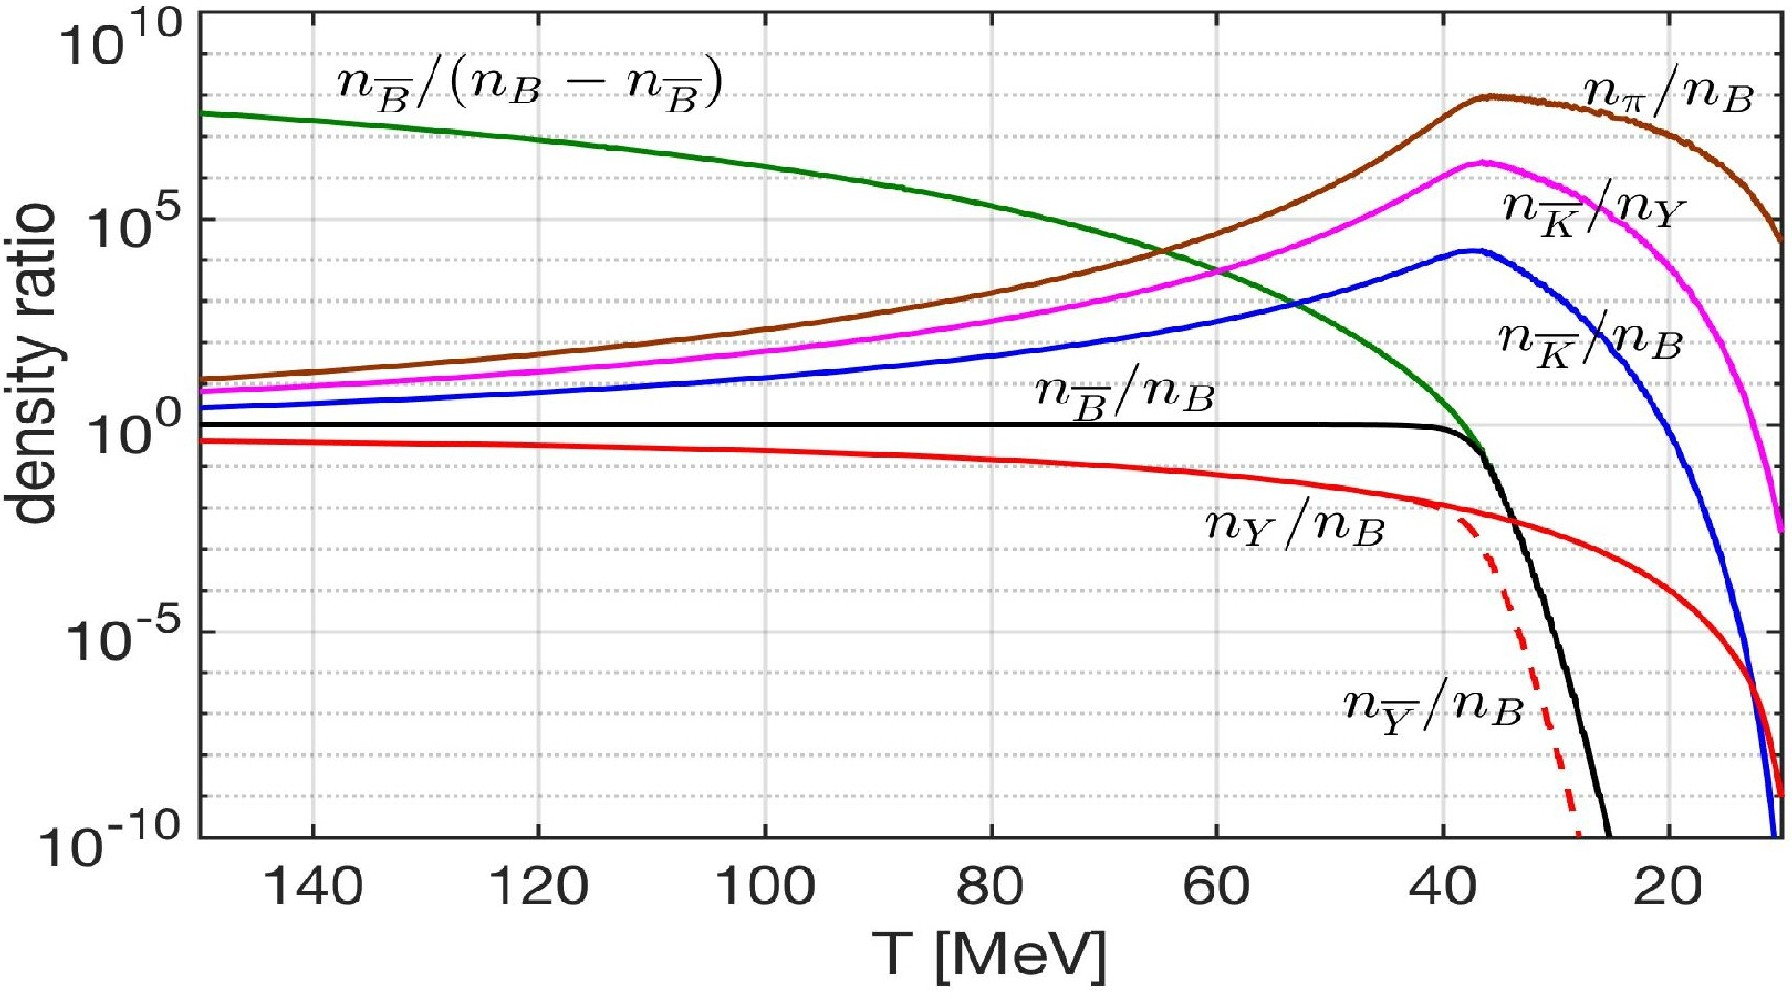
\includegraphics[width=0.9\linewidth]{./plots/Meson_Baryon_density_ratio_C.jpg}}
\caption{Ratios of hadronic particle number densities  with baryon $B$ yields as a function of temperature $150\MeV> T>10\MeV$: Pions $\pi$ (brown line), kaons $K( q\bar s)$ (blue), antibaryon $\overline B$ (black), hyperon $Y$ (red) and anti-hyperons $\overline Y$ (dashed red). Also shown $\overline K/Y$(purple). \cccite{Rafelski:2023emw}. \radapt{Yang:2021bko}}
\label{EquilibPartRatiosFig} 
\end{figure}
%%%%%%%%%%%%%%%%%%%%%%%%%%%
\index{strangeness!equilibrium among baryons and mesons} 

For $20.8\MeV>T$, the  baryon abundance becomes dominant over strange mesons $n_{\overline K}/n_B<1$, which implies that the strange meson is embedded in a large background of baryons, and the exchange reaction $\overline{K}+N\rightarrow \Lambda+\pi$ can re-equilibrate kaons and hyperons in the temperature range; therefore strangeness symmetry $s=\bar s$ can be maintained. For $12.9\MeV>T$ we have $n_Y/n_B>n_{\overline K}/n_B$, now the still existent tiny abundance of strangeness is found predominantly in hyperons.

%%%%%%%%%%%%%%%%%%%%%%%%%%%%%%%%%
\para{Strangeness dynamic population}\index{strangeness!dynamic population}
Given the equilibrium abundances of hadrons in the epoch of interest is $150\MeV\ge T\ge 10\MeV$ we turn now to study the freeze-out temperature for different particles and strangeness  by comparing the relevant reaction rates with each other and with the Hubble expansion rate.  We will need to explore a large number of reactions, going well beyond the relative simplicity of the case of QGP phase of matter. We find that strangeness is kept in equilibrium in the primordial Universe down until $T\approx 13\MeV$. This study addresses non-interacting particles, nuclear interactions can be many times greater compared to this temperature. Thus further exploration of this result seems necessary in the future.

Let us first consider an unstable strange particle $S$ decaying into two particles $1$ and $2$, which themselves have no strangeness content. In a dense and high-temperature plasma with particles $1$ and $2$ in thermal equilibrium, the inverse reaction populates the system with particle $S$. This is written schematically as
\begin{align}
 S\Longleftrightarrow1+2,\qquad \mathrm{Example}: K^0\Longleftrightarrow\pi+\pi\,.
\end{align}
As long as both decay and production reactions are possible, particle $S$ abundance remains in thermal equilibrium; as already discussed this balance between production and decay rates is the `detailed balance'.

Once the primordial Universe expansion rate $1/H$ overwhelms the strongly temperature dependent back-reaction and the back reaction freeze-out, then the decay $S\rightarrow 1+2$ occurs out of balance and particle $S$ disappears rather rapidly from the inventory. 

Second on our list are the two-on-two strangeness producing and burnup reactions. These have a significantly higher strangeness production reaction threshold, thus especially near to strangeness decoupling their influence is negligible. Such reactions are more important near the QGP hadronization temperature $T_H\simeq 150\MeV$. Typical  strangeness exchange reaction is $\mathrm{K}+N\leftrightarrow \Lambda+\pi$, (see Chapter 18 in~Ref.\,\cite{Letessier:2002ony}).

In~\rf{Strangeness_map2} we show some reactions relevant to strangeness evolution in the considered Universe evolution epoch $150\MeV\ge T\ge 10\MeV$ and their pertinent reaction strength. Specifically:
\begin{itemize}
\item
We study strange quark abundance in baryons and mesons, considering both open and hidden strangeness (hidden: $s\bar s$-content). Important source reactions are $l^-+l^+\rightarrow\phi$, $\rho+\pi\rightarrow\phi$, $\pi+\pi\rightarrow K_\mathrm{S}$, $\Lambda \leftrightarrow \pi+ N$, and $\mu^\pm+\nu\rightarrow K^\pm$. 
\item
Muons and pions are coupled through electromagnetic reactions $\mu^++\mu^-\leftrightarrow\gamma+\gamma$ and $\pi\leftrightarrow\gamma+\gamma$ to the photon background and retain their chemical equilibrium until the temperature $T =4$\, MeV and $T=5\MeV$, respectively~\cite{Rafelski:2021aey,Kuznetsova:2008jt}. The large $\phi\leftrightarrow K+K$ rate assures $\phi$ and $K$ are in relative chemical equilibrium.
\end{itemize}

%%%%%%%%%%%%%%%%%%%%%%%%%%%%%%%%%%%%%%%
\begin{figure} 
\centerline{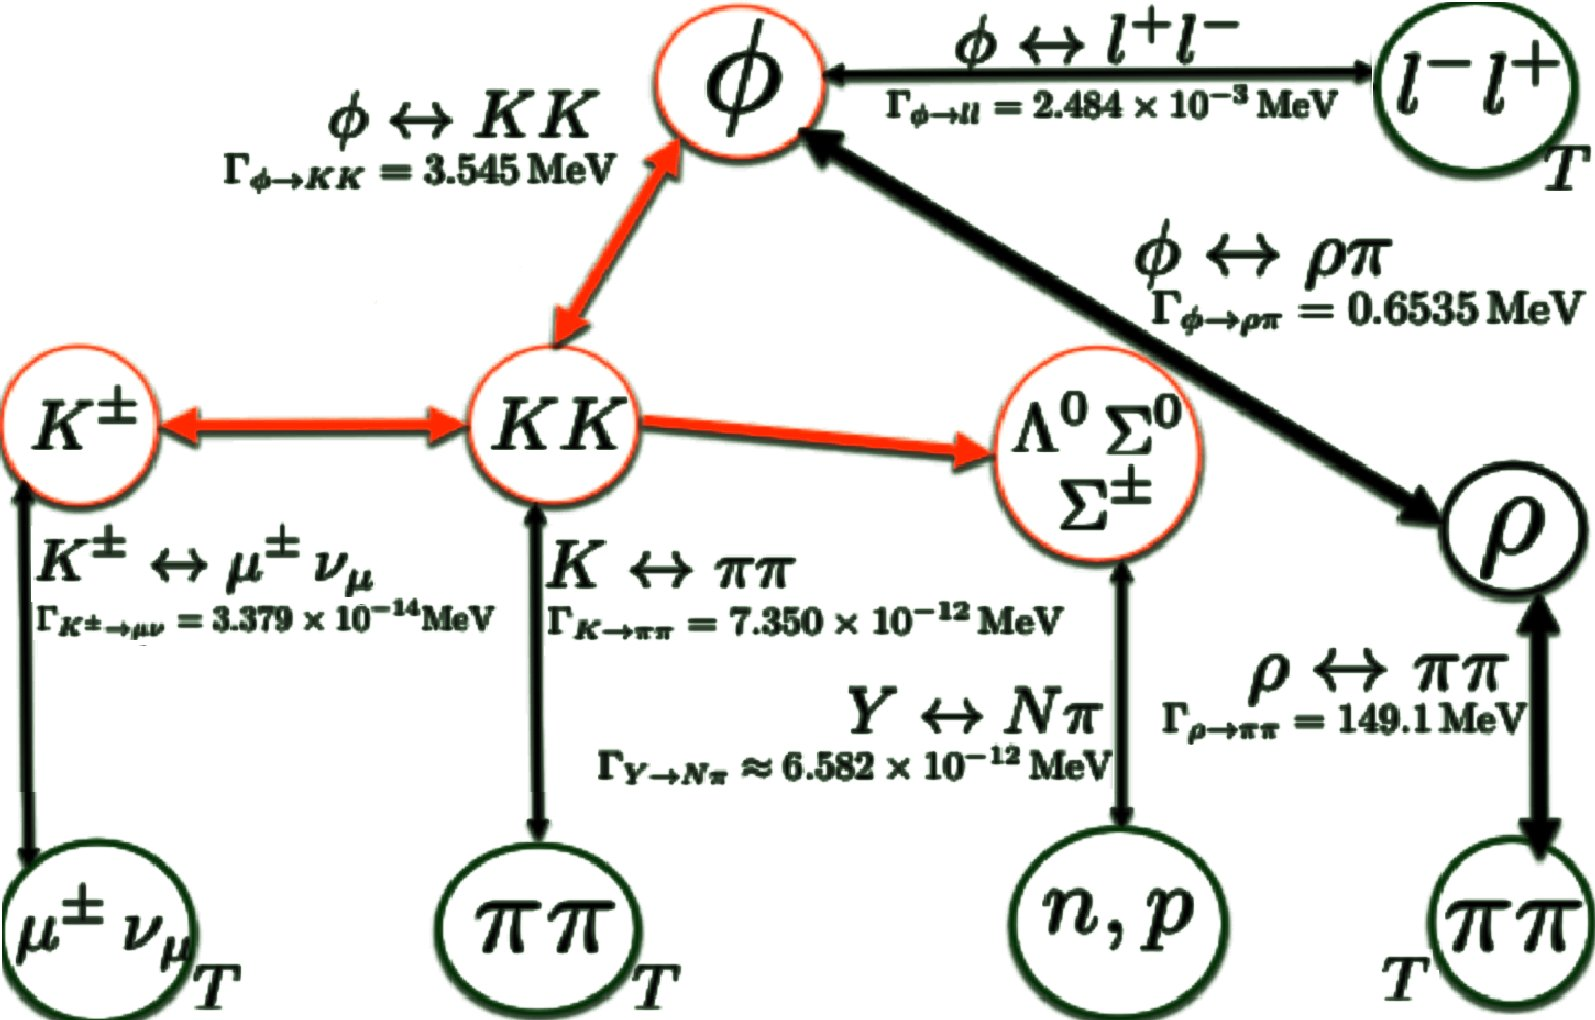
\includegraphics[width=0.9\linewidth]{./plots/Strangeness002_newJ.jpg}}
\caption{The strangeness abundance changing reactions in the primordial Universe. The red circles show strangeness carrying hadronic particles; red thick lines denote effectively instantaneous reactions. Black thick lines show relatively strong hadronic reactions. The reaction rates required to describe strangeness time evolution are presented in Ref.~\cite{Rafelski:2020ajx}. \cccite{Rafelski:2023emw}. \radapt{Yang:2024ret,Yang:2021bko}}
\label{Strangeness_map2} 
\end{figure}
%%%%%%%%%%%%%%%%%%%%%%%%%%%%%%%%%%%%

In order to determine where exactly strangeness disappears from the Universe inventory, we explore the magnitudes of different rates of production and decay processes in mesons and hyperons.
 
%%%%%%%%%%%%%%%%%%%%%%%%%%%%%%%%%%%%%
\para{Strangeness creation and annihilation rates in mesons}
From~\rf{Strangeness_map2} in the meson domain, the relevant interaction rates competing with Hubble time are the reactions\index{strangeness!mesons production rate}
\begin{align}
 &\pi+\pi\leftrightarrow K\,,\quad\mu^\pm+\nu\leftrightarrow K^\pm\,,\quad l^++l^-\leftrightarrow\phi\,,\\
 &\rho+\pi\leftrightarrow\phi\,,\quad \pi+\pi\leftrightarrow\rho\,.
\end{align}
The thermal reaction rate per time and volume for two body-to-one particle reactions $1+2\rightarrow 3$ has been presented before~\cite{Koch:1986ud,Kuznetsova:2008jt,Kuznetsova:2010pi}. 

In full kinetic and chemical equilibrium, the reaction rate per time per volume can be written as~\cite{Kuznetsova:2010pi} :\index{inverse decay rate}
\begin{align}
&R_{12\to 3}=\frac{g_3}{(2\pi)^2}\,\frac{m_3}{\tau^0_3}\,\int^\infty_0\frac{p^2_3dp_3}{E_3}\frac{e^{E_3/T}}{e^{E_3/T}\pm1}\Phi(p_3)\;,
\end{align}
where $\tau^0_3$ is the vacuum lifetime of particle $3$. The positive sign `$+$' is for the case when particle $3$ is a boson, and negative sign `$-$' for a fermion. The function $\Phi(p_3)$ for the nonrelativistic limit $m_3\gg p_3,T$ can be written as 
\begin{align}
\Phi(p_3\to0)=2\frac{1}{(e^{E_1/T}\pm1)(e^{E_2/T}\pm1)}.
\end{align}

Considering the Boltzmann limit, the thermal reaction rate per unit time and volume becomes
\begin{align}
\label{Thermal_Rate}
R_{12\rightarrow3}=\frac{g_3}{2\pi^2}\left(\frac{T^3}{\tau^0_3}\right)\left(\frac{m_3}{T}\right)^2\,K_1(m_3/T),
\end{align}
where $K_1$ is the modified Bessel functions of integer order `$1$'. 

In order to compare the reaction time with Hubble time $1/H$, it is convenient to define the relaxation time for the process $1+2\rightarrow 3$ as follows:
\begin{align}
\label{Reaction_Time}
\tau_{12\rightarrow 3}\equiv\frac{n^{eq}_{1}}{R_{12\rightarrow n}}\,,\quad
n^{eq}_1=\frac{g_1}{2\pi^2}\int_{m_1}^\infty\!\!\!\!dE\,\frac{E\,\sqrt{E^2-m_1^2}}{\exp{\left(E/T\right)}\pm1}\;, 
\end{align}
where $n^{eq}_1$\,is the thermal equilibrium number density of particle\,$1$ with the `heavy' mass $m_1>T$. Combining \req{Thermal_Rate} with \req{Reaction_Time} we obtain
\begin{align}\label{RelaxationTime}
&\frac{\tau_{12\rightarrow3}}{ \tau^0_3}= 
\frac{2\pi^2 n^{eq}_1/T^3}{g_3(m_3/T)^2\,K_1(m_3/T)}\,, \quad 
n^{eq}_1\simeq g_1\left(\frac{m_1 T}{2\pi}\right)^{3/2}e^{-m_1/T}\,,
\end{align}
where, conveniently, the relaxation time does not depend on the abundant and often relativistic heat bath component $2$, \eg\ $l^\pm,\pi,\nu,\gamma$. The density of heavy particles\,$1$\,and\,$3$ can in general be well approximated using the leading and usually nonrelativistic Boltzmann term as shown above.

In general, the reaction rates for inelastic collision process capable of changing particle number, for example $\pi\pi\to K^0$, is suppressed by the factor $\exp{(-m_{K^0}/T)}$. On the other hand, there is no suppression for the elastic momentum and energy exchanging particle collisions in plasma. In general for the case $m\gg T$, the dominant collision term in the relativistic Boltzmann equation is the elastic collision term, keeping all heavy particles in kinetic energy equilibrium with the plasma. This allows us to study the particle abundance in plasma presuming the energy-momentum statistical distribution  equilibrium shape exists.  This insight was discussed in detail in the preparatory phase of laboratory exploration of hot hadron and quark matter, see~\cite{Koch:1986ud}. 

In order to study the particle abundance in the Universe when $m\gg T$, instead of solving the exact Boltzmann equation, we can separate the fast energy-momentum equilibrating collisions from the slow particle number changing inelastic collisions. This approach makes it possible to explore the rates of inelastic collision and compare the relaxation times of particle production in all relevant reactions with the Universe expansion rate at a fixed temperature which governs the shape of particle distributions.

It is common to refer to particle freeze-out as the epoch where a given type of particle ceases to interact with other particles. In this situation the particle abundance decouples from the cosmic plasma, a chemical nonequilibrium and even complete abundance disappearance of this particle can accompany this; the condition for the given reaction $1+2\rightarrow 3$ to decouple is
\begin{align}
\tau_{12\rightarrow 3}(T_f)=1/H(T_f),
\end{align}
where $T_f$ is the freeze-out temperature.

In the epoch of interest, $150\MeV>T>10\MeV$, the Universe is dominated by radiation and effectively massless matter behaving like radiation. The Hubble parameter can be obtained from the Hubble equation and written as~\cite{Kolb:1990vq}
\begin{align}\label{H2g}
H^2=H^2_{rad}\left(1+\frac{\rho_{\pi,\,\mu,\,\rho}}{\rho_\mathrm{rad}}+\frac{\rho_\mathrm{strange}}{\rho_\mathrm{rad}}\right)=\frac{8\pi^3G_\mathrm{N}}{90}g^e_\ast T^4,\qquad H^2_\mathrm{rad}=\frac{8\pi G_\mathrm{N}\,\rho_\mathrm{rad}}{3},
\end{align}
where: $g^e_\ast$ is the total number of effective relativistic `energy' degrees of freedom; $G_\mathrm{N}$ is the Newtonian constant of gravitation; the `radiation' energy density includes $\rho_\mathrm{rad}=\rho_\gamma+\rho_\nu+\rho_{e^\pm}$ for photons, neutrinos, and massless electrons(positrons). The massive-particle correction is $\rho_{\pi,\,\mu,\,\rho}=\rho_\pi+\rho_\mu+\rho_\rho$; and at highest $T$ of interest, also of (minor) relevance, $\rho_\mathrm{strange}=\rho_{K^0}+\rho_{K^\pm}+\rho_{K^\ast}+\rho_{\eta}+\rho_{\eta^\prime}$.
Equating $1/H$ to the computed reaction rate we obtain the freeze-out temperature $T_f$. 

When considering the reaction rates and quoting $T_f$,   we must check allowing for a finite reaction time how sudden the freeze-out happens. We refer to this temperature uncertainty as  $\Delta T_f$, which by a simple scale consideration can be defined by
\begin{equation}\label{eq:DeltaT}
\Delta T_f\simeq \frac{1}{R(T_f)}\times \frac{dT}{dt}\,. 
\end{equation}
$R$\,[MeV] is the value of reaction rate at freeze-out. The greater is the rate $R_f$ the sharper is the freeze-out, thus smaller $\Delta T_f$.\index{freeze-out!uncertainty}

For the temperature range $50\MeV>T>5\MeV$, we have $10^{-1}<dT/dt<10^{-4}\MeV$/$\mu$s. We estimate the  width of freeze-out temperature interval $\Delta T_f$ using reaction rates for $dt$ as follows
\begin{align}
\frac{1}{\Delta T_f}\equiv \left[\frac{1}{(\Gamma_{12\to3}/H)}\frac{d(\Gamma_{12\to3}/H)}{dT}\right]_{T_f},\quad \Gamma_{12\to3}\equiv\frac{1}{\tau_{12\to3}}.
\end{align}
Using \req{H2g} and \req{RelaxationTime} and considering the temperature range $50\MeV>T>5\MeV$ with $g^e_\ast\approx\mathrm{constant}$ we obtain using the Boltzmann approximation to describe the massive particles\,$1$\,and\,$3$
\begin{align}\label{DeltaFreezeout}
 \frac{\Delta T_f}{ T_f} \approx\frac{T_f }{ m_3 - m_1 -2T_f}\,,\quad m_3 - m_1>> T_f\,.
\end{align}
The width of freeze-out domain is shown in the right column in Table~\ref{FreezeoutTemperature_table}. We see a range of $2$-$10\%$. Therefore it is nearly justified to consider as a decoupling condition in time the value of temperature at which the pertinent rate crosses the Hubble expansion rate, see~\rf{reaction_time_tot}.\index{freeze-out!duration}
 
%%%%%%%%%%%%%%%%%%%%%%%%%%%
\begin{table} 
\centering
\begin{tabular}{c| c| c}
\hline\hline
Reactions &Freeze-out $T_f$\,[MeV] & {Uncertainty $\Delta T_f$\,[MeV]} \\
\hline
$\mu^\pm\nu\rightarrow K^\pm$ & $T_f=33.8\MeV$ & {$3.5$ \,MeV}\\ 
\hline
$e^+e^-\rightarrow \phi$ & $T_f=24.9\MeV$ &{$0.6\MeV$}\\
$\mu^+\mu^-\rightarrow\phi$ & $T_f=23.5\MeV$ &{$0.6\MeV$}\\
\hline
 $\pi\pi\rightarrow K$ & $T_f=19.8\MeV$&{$1.2\MeV$}\\
\hline
$\pi\pi\rightarrow\rho$ & $T_f=12.3\MeV$&{$0.2\MeV$}\\
\hline\hline
\end{tabular}
\caption{Strangeness producing reactions in primordial Universe, their freeze-out temperature $T_f$; and temperature uncertainty $\Delta T_f$}
\label{FreezeoutTemperature_table} 
\end{table}
%%%%%%%%%%%%%%%%%%%%%%%%%%%%%%%%%%%%%%

%%%%%%%%%%%%%%%%%%%%%%%%%%%%%%%%%%%%%%%%%
\begin{figure}
%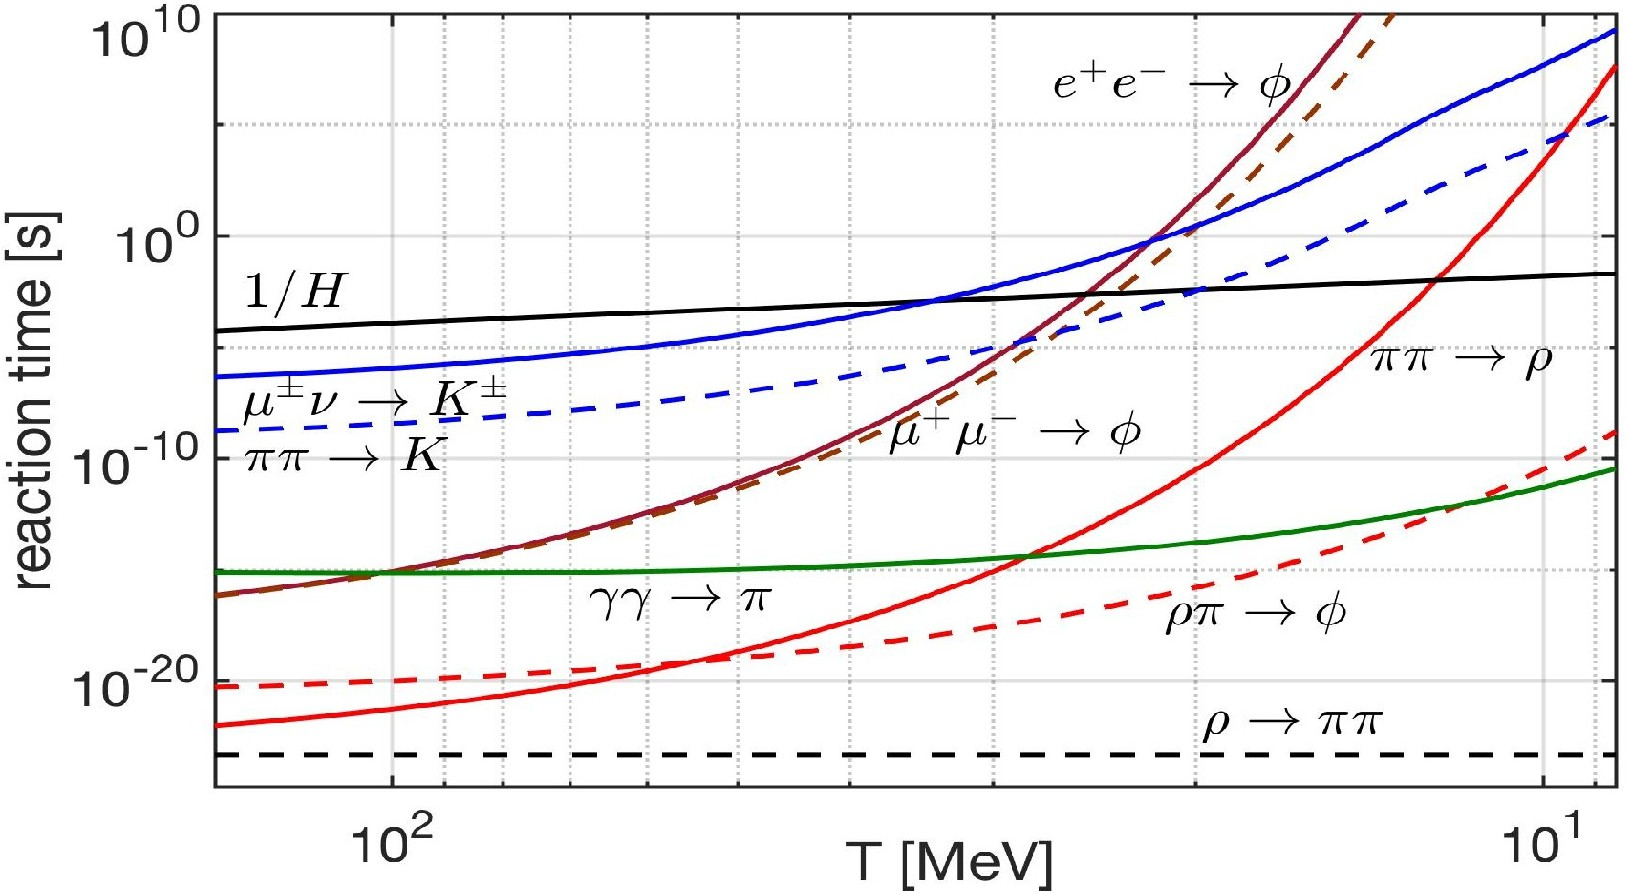
\includegraphics[width=0.95\linewidth]{./plots/Strangeness_Hubble_C.jpg}
\centerline{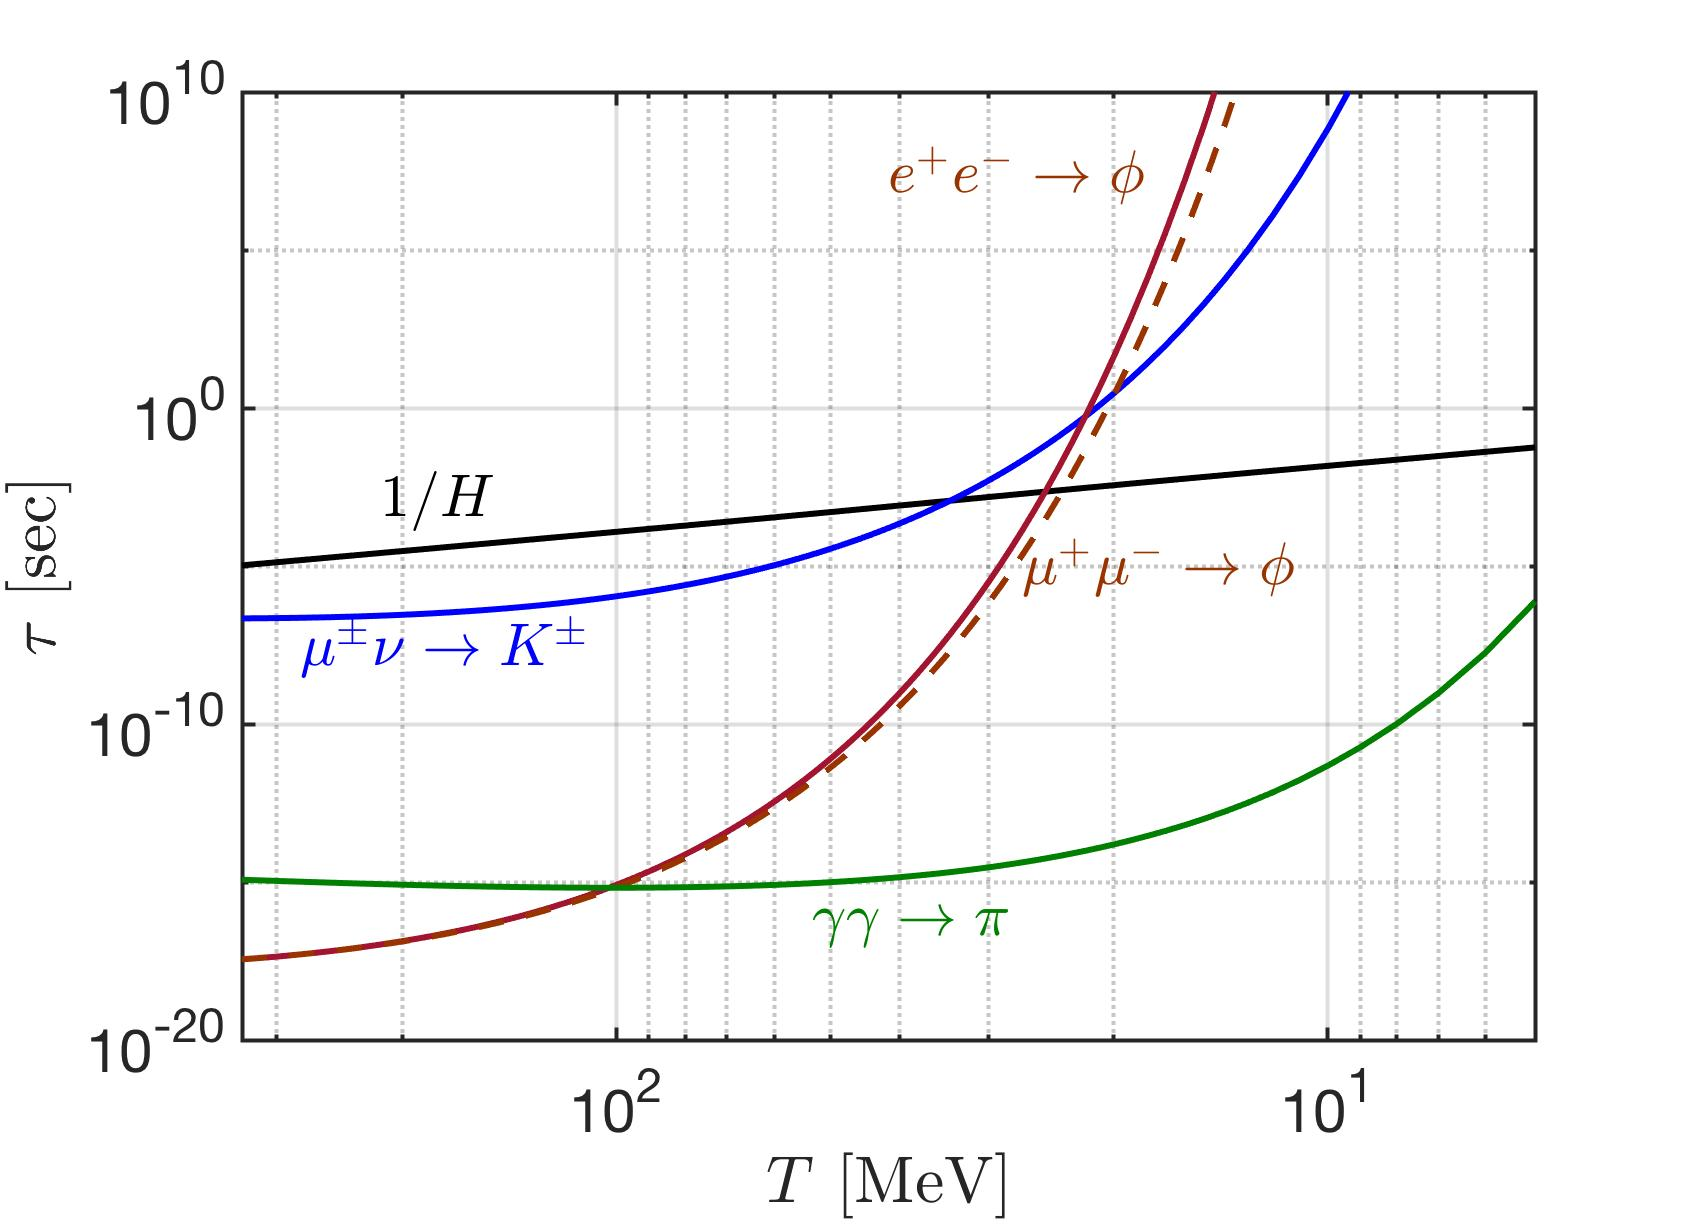
\includegraphics[width=0.9\linewidth]{./plots/Strangeness_Hubble002.jpg}}
\centerline{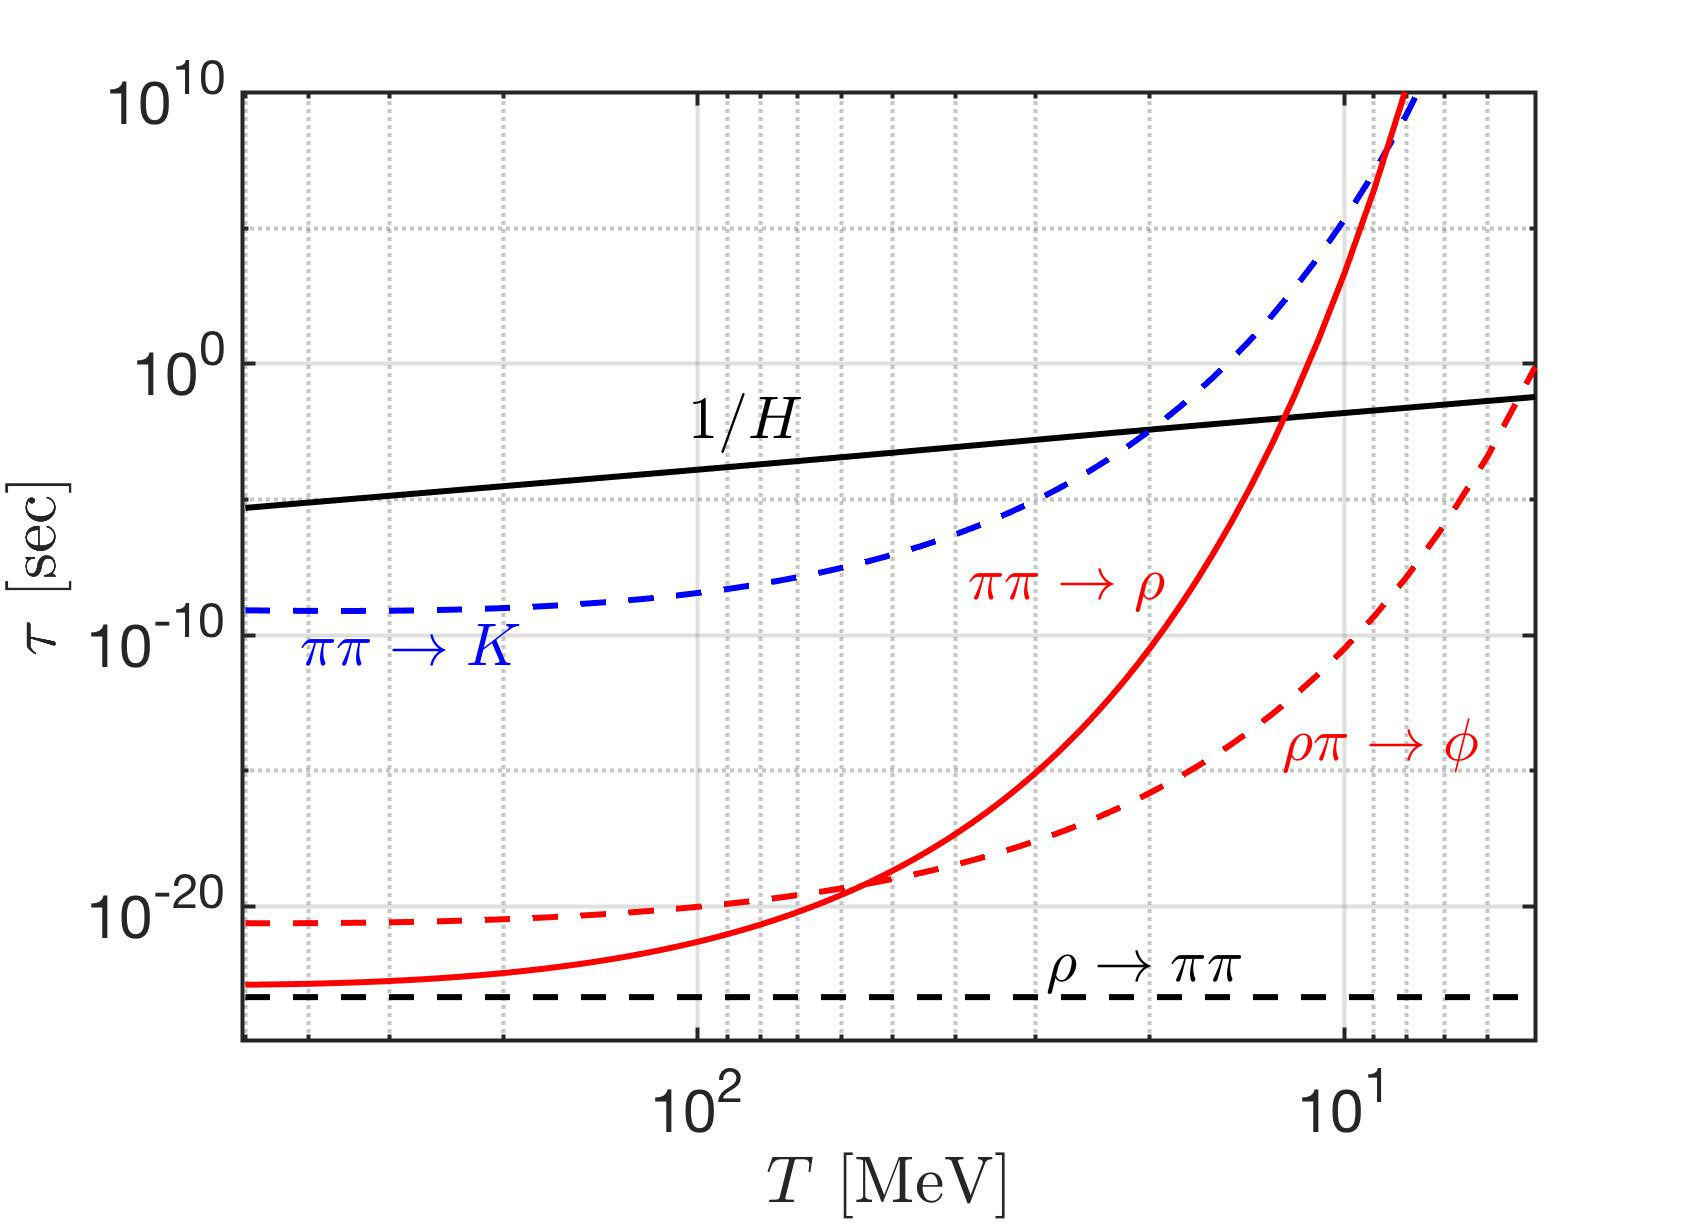
\includegraphics[width=0.9\linewidth]{./plots/Strangeness_Hubble003.jpg}}
\caption{Hadronic relaxation reaction times, see \req{Reaction_Time}, as a function of temperature $T$, are compared to Hubble time $1/H$ (black solid line). At bottom the horizontal black-dashed line is the natural (vacuum) lifespan of $\rho$. \cccite{Rafelski:2023emw}. \radapt{Yang:2024ret,Yang:2021bko}}
\label{reaction_time_tot} 
\end{figure}
%%%%%%%%%%%%%%%%%%%%%%%%

In~\rf{reaction_time_tot} we plot the hadronic reaction relaxation times $\tau_{i}$ in the meson sector as a function of temperature compared to Hubble time $1/H$. We note that the weak interaction reaction $\mu^\pm+\nu_{\mu}\rightarrow K^\pm$ becomes slower compared to the Universe expansion near temperature $T_f^{K^\pm}=33.8\MeV$, signaling the onset of abundance nonequilibrium for $K^\pm$. For $T<T_f^{K^\pm}$, the reactions $\mu^\pm+\nu_{\mu}\rightarrow K^\pm$ decouples from the cosmic plasma; the corresponding detailed balance can be broken and the decay reactions $K^\pm\rightarrow\mu^\pm+\nu_{\mu}$ are acting like a (small) ``hole'' in the strangeness abundance ``pot''. If other strangeness production reactions did not exist, strangeness would disappear as the Universe cools below $T_f^{K^\pm}$. However, there are other reactions: $l^++l^-\leftrightarrow\phi$, $\pi+\pi\leftrightarrow K$, and $\rho+\pi\leftrightarrow\phi$ can still produce the strangeness in cosmic plasma and the rate is very large compared to the weak interaction decay.

In Table~\ref{FreezeoutTemperature_table} we also show the characteristic strangeness reactions and their freeze-out temperatures in the primordial Universe. The intersection of strangeness reaction times with $1/H$ occurs for $l^-+l^+\rightarrow\phi$ at $T_f^\phi=25\sim23\MeV$, and for $\pi+\pi\rightarrow K$ at $T_f^K=19.8\MeV$, for $\pi+\pi\rightarrow\rho$ at $T_f^\rho=12.3\MeV$. The reactions $\gamma+\gamma\rightarrow\pi$ and $\rho+\pi\leftrightarrow\phi$ are faster compared to $1/H$. However, the $\rho\to\pi+\pi$ lifetime (black dashed line in~\rf{reaction_time_tot}) is smaller than the reaction $\rho+\pi\leftrightarrow\phi$; in this case, most of $\rho$-meson decays faster, thus are absent and cannot contribute to the strangeness creation in the meson sector. Below the temperature $T<20\MeV$, all the detail balances in the strange meson reactions are broken and the strangeness in the meson sector should disappear rapidly, were it not for the small number of baryons present in the Universe.

%%%%%%%%%%%%%%%%%%%%%%%%%%%%%%%%%%%%%%%%%%%%
\para{Strangeness production and exchange rates involving hyperons}\index{strangeness!hyperons}
In order to understand strangeness in hyperons in the baryonic domain, we now consider the strangeness production reaction $\pi +N\rightarrow K+\Lambda$, the strangeness exchange reaction $\overline{K}+N\rightarrow \Lambda+\pi$; and the strangeness decay $\Lambda\rightarrow N+\pi$. The competition between different strangeness reactions allows strange hyperons and antihyperons to influence the dynamic nonequilibrium condition, including development of $\langle s-\bar s\rangle \ne 0$.

To evaluate the reaction rate in two-body reaction $1+2\rightarrow3+4$ in the Boltzmann approximation we can use the reaction cross section $\sigma(s)$ and the relation~\cite{Letessier:2002ony}:\index{hyperon!production rate}
\begin{align}
R_{12\rightarrow34}=\frac{g_1g_2}{32\pi^4}\frac{T}{1+I_{12}}\!\!\int^\infty_{s_{th}}\!\!\!\!ds\,\sigma(s)\frac{\lambda_2(s)}{\sqrt{s}}\!K_1\!\!\left({\sqrt{s}}/{T}\right),
\end{align}
where $K_1$ is the Bessel function of order $1$ and the function $\lambda_2(s)$ is defined as
\begin{align}
\lambda_2(s)=\left[s-(m_1+m_2)^2\right]\left[s-(m_1-m_2)^2\right],
\end{align}
with $m_1$ and $m_2$, $g_1$ and $g_2$ as the masses and degeneracy of the initial interacting particle. The factor $1/(1+I_{12})$ is introduced to avoid double counting of indistinguishable pairs of particles; we have $I_{12}=1$ for identical particles and $I_{12}=0$ for others. 

The thermal averaged cross sections for the strangeness production and exchange processes are about $\sigma_{\pi N\rightarrow K\Lambda}\sim0.1\,\mathrm{mb}$ and $\sigma_{\overline{K}N\rightarrow \Lambda\pi}=1\sim3\,\mathrm{mb}$ in the energy range in which we are interested~\cite{Koch:1986ud}. The cross section can be parameterized as follows:\\
1) For the cross section $\sigma_{\overline{K}N\rightarrow \Lambda\pi}$ we use~\cite{Koch:1986ud}
 \begin{align}
 \sigma_{\overline{K}N\rightarrow \Lambda\pi}=\frac{1}{2}\left(\sigma_{K^-p\rightarrow \Lambda\pi^0}+\sigma_{K^-n\rightarrow \Lambda\pi^-}\right)\,.
\end{align}
Here the experimental cross sections can be parameterized as 
\begin{align}
&\sigma_{K^-p\rightarrow \Lambda\pi^0}\!\!=\!\!\left(\begin{array}{l}\!\!1479.53\mathrm{mb}\!\cdot\!\exp{\left(\frac{-3.377\sqrt{s}}{\mathrm{GeV}}\right)},\; \mathrm{for}\,\sqrt{s_m}\!\!<\!\!\sqrt{s}\!<\!3.2\mathrm{GeV} \\ \\0.3\mathrm{mb}\!\cdot\!\exp{\left(\frac{-0.72\sqrt{s}}{\mathrm{GeV}}\right)},\; \mathrm{for}\sqrt{s}>3.2\mathrm{GeV}\end{array}\right.\\
&\sigma_{K^-n\rightarrow \Lambda\pi^-}\!\!=\!\!1132.27\mathrm{mb}\!\cdot\!\exp{\left(\frac{-3.063\sqrt{s}}{\mathrm{GeV}}\right)},\; \mathrm{for}\sqrt{s}>1.699\mathrm{GeV},
\end{align}
where $\sqrt{s_m}=1.473\GeV$.\\
2) For the cross section $\sigma_{\pi N\rightarrow K\Lambda}$ we use~\cite{Cugnon:1984pm}
\begin{align}
&\sigma_{\pi N\rightarrow K\Lambda}=\frac{1}{4}\times\sigma_{\pi p\rightarrow K^0\Lambda}\,.
\end{align}
The experimental $\sigma_{\pi p\rightarrow K^0\Lambda}$ can be approximated as follows
\begin{align}
\sigma_{\pi p\rightarrow K^0\Lambda}=\left(\begin{array}{l}\frac{0.9\mathrm{mb}\cdot\left(\sqrt{s}-\sqrt{s_0}\right)}{0.091\mathrm{GeV}},\; \mathrm{for} \sqrt{s_0}<\sqrt{s}<1.7\mathrm{GeV} \\ \\ \frac{90\mathrm{MeV\cdot mb}}{\sqrt{s}-1.6\mathrm{GeV}},\; \mathrm{for}\sqrt{s}>1.7\mathrm{GeV},\end{array}\right.
 \end{align}
 with $ \sqrt{s_0}=m_\Lambda+m_K$. 

Given the cross sections, we obtain the thermal reaction rate per volume for strangeness exchange reaction seen in~\rf{Lambda_Rate_volume.fig}. We see that near to $T=20\MeV$, the dominant reactions for the hyperon $\Lambda$ production is $\overline{K}+N\leftrightarrow\Lambda+\pi$. At the same time, the $\pi+\pi\to K$ reaction becomes slower than Hubble time and kaon $K$ decay rapidly in the primordial Universe. However, the anti-kaons $\overline K$ produce the hyperon $\Lambda$ because of the strangeness exchange reaction $\overline{K}+N\rightarrow\Lambda+\pi$ in the baryon-dominated Universe. We have strangeness in $\Lambda$ and it disappears from the Universe via the decay $\Lambda\rightarrow N+\pi$. Both strangeness and anti-strangeness disappear because of the $K\rightarrow\pi+\pi$ and $\Lambda\rightarrow N+\pi$, while the strangeness abundance $s = \bar{s}$ in the primordial Universe remains.

%%%%%%%%%%%%%%%%%%%%%%%%%%%%%%%%
\begin{figure} 
\centerline{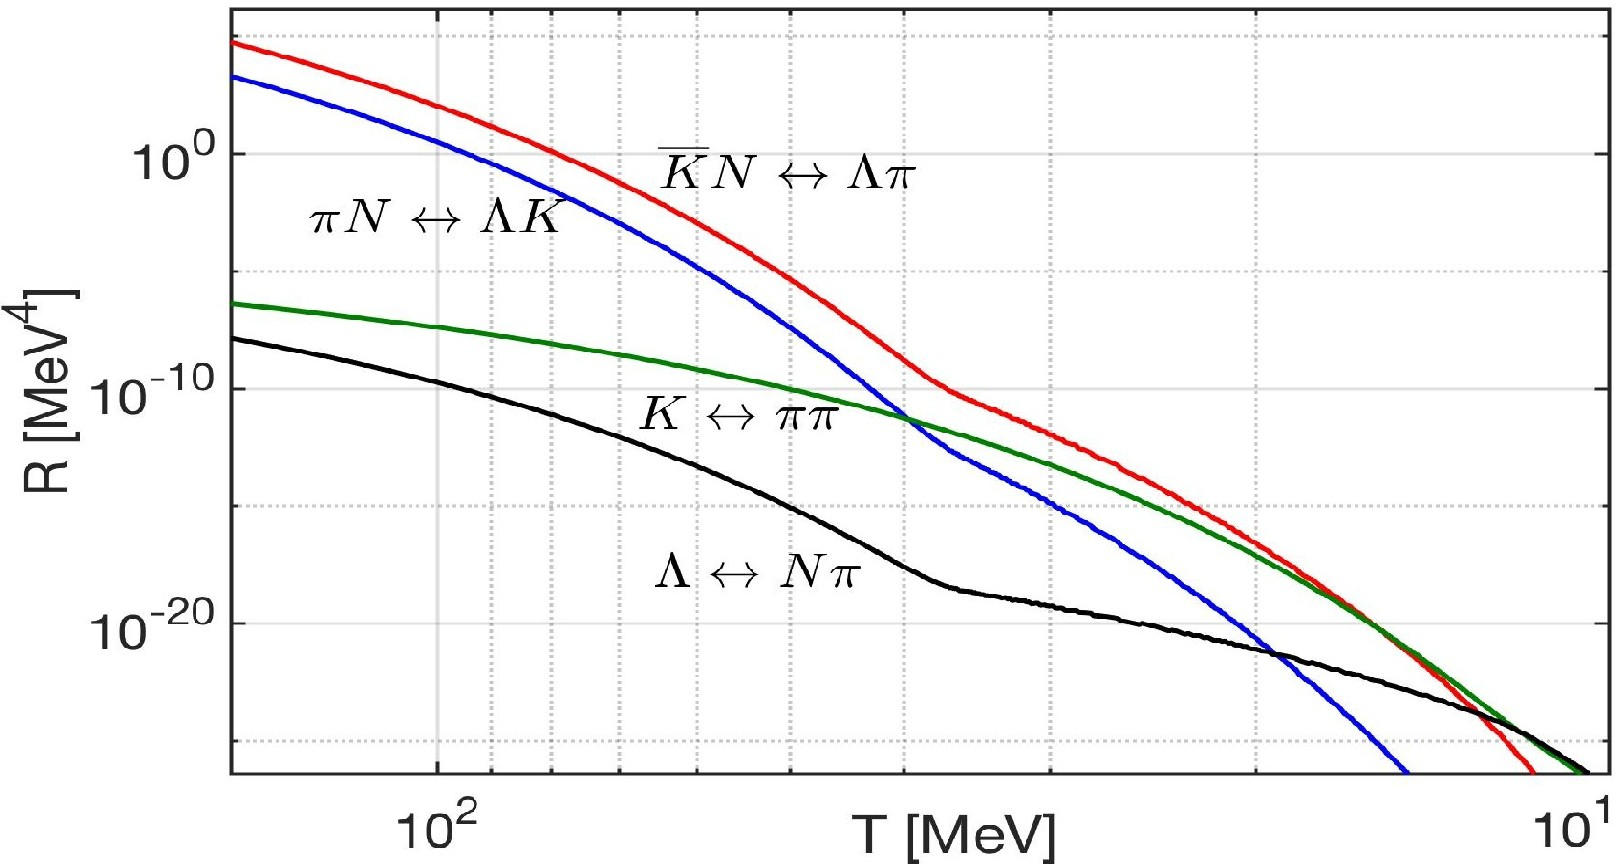
\includegraphics[width=0.9\linewidth]{./plots/NewHyperonRate_C.jpg}}
\caption{Thermal reaction rate $R$ per volume and time for important hadronic strangeness production and exchange processes as a function of temperature $150\MeV> T>10\MeV$ in the primordial Universe. \cccite{Rafelski:2023emw}. \radapt{Yang:2024ret,Yang:2021bko}}
\label{Lambda_Rate_volume.fig} 
\end{figure}
%%%%%%%%%%%%%%%%%%%%%%%%%%%%%%%%%%%%

Near to $T=12.9\MeV$ the reaction $\Lambda+\pi\rightarrow\overline{K}+N$ becomes slower than the strangeness decay $\Lambda\leftrightarrow N+\pi$ and shows that at the low temperature the $\Lambda$ particles are still in equilibrium via the reaction $\Lambda\leftrightarrow N+\pi$ and little strangeness remains in the $\Lambda$. Then strangeness abundance becomes asymmetric $s\gg \bar{s}$, which implies that the assumption for strangeness conservation can only be valid until the temperature $T\sim13\MeV$. Below this temperature a new regime opens up in which the tiny residual strangeness abundance is governed by weak decays with no re-equilibration with mesons. Also, in view of baron asymmetry, $\langle s-\bar s\rangle \ne 0$.

\chapter
{Strangeness abundance in cosmic plasma}
\label{Strangeness}
%{Heavy-quark in primordial QGP: after hadronization}
As the Universe expanded and cooled down to the hadronization temperature $T_H\approx150$ MeV, the primordial QGP underwent a phase transformation called hadronization. This transition resulted in the confinement of the strong force, causing quarks and gluons to combine and form matter 
and antimatter. After hadronization, one may think the relatively short lived massive hadrons decay rapidly and disappear from the Universe. However, the most abundant hadrons, pions $\pi(q\bar q)$, can be produced via their inverse decay process $\gamma\gamma\rightarrow\pi^0$ and retain their chemical equilibrium until temperature $T=3\sim5$ MeV~[\cite{Kuznetsova:2008jt}]. 

Following the idea and the framework presented by~[\cite{Kuznetsova:2008jt}], we investigate the strange particle composition of the expanding early Universe in the epoch $150\,\mathrm{MeV}\ge T\ge 10$\,MeV, and examine the freeze-out temperature for strangeness-producing  by comparing the relevant reaction rates to the Hubble expansion rate. We show that strangeness is kept in equilibrium via weak, electromagnetic, and strong interactions in the early Universe until $T\approx13$ MeV.


 
%~~~~~~~~~~~~~~~~~~~~~~~~~~~~~~~~~~~~~~~~~~~~~~~~~



%~~~~~~~~~~~~~~~~~~~~~~~~~~~~~~~~~~~~~~~~~~~~~~~~~

\section{Chemical equilibrium in the hadronic Universe}
%In this section we will focus on the following:
%\begin{itemize}
%    \item Chemical potentials of $\mu_B$ and $\mu_s$
%    \item Composition of universe (strangeness abundance)
%\end{itemize}

In this section, we explore the Universe composition assuming both kinetic and particle abundance equilibrium (chemical equilibrium) by considering the charge neutrality and prescribed conserved baryon-per-entropy-ratio ${(n_B-n_{\overline{B}})}/{\sigma}$ to determine the baryon chemical potential $\mu_B$~[\cite{Fromerth:2012fe,Rafelski:2013yka}]. With the chemical potential as a function of temperature, we can obtain the particle number densities for different species and study their composition in the early Universe.

We improve the prior work~[\cite{Fromerth:2012fe}] by considering the conserved entropy per baryon ratio with conservation of strangeness in the early Universe. To study the baryon and strange quark chemical potential, it is convenient to introduce the chemical fugacity for strangeness $\lambda_s$ and quark $\lambda_q$ as follows:
\begin{align}
\lambda_s=\exp(\mu_s/T)\,\quad \lambda_q=\exp(\mu_B/3T),
\end{align}
where $\mu_s$ and $\mu_B$ are the chemical potential of strangeness and baryon, respectively. For the quark fagucity $\lambda_q$, we divide the chemical potential of baryons by 3 as an approximation for quark chemical potential. Imposing the conservation of strangeness  
$\langle s-\bar s \rangle=0$, we have, when the baryon chemical potential does not vanish the chemical potential of strangeness in the early Universe satisfying (see Section 11.5 in \,[\cite{Letessier:2002ony}])
\begin{align}\label{museq}
\lambda_s=\lambda_q\sqrt{\frac{F_K+\lambda^{-3}_q\,F_Y}{F_K+\lambda^3_q\,F_Y}}.
\end{align}
where we employ the phase-space function $F_i$ for sets of nucleon $N$, kaon $K$, and hyperon $Y$ particles defined as (see [\cite{Letessier:2002ony}], Section 11.4):
\begin{align}
&F_N=\sum_{N_i}\,g_{N_i}W(m_{N_i}/T)\;, \quad N_i=n, p, \Delta(1232),\\
&F_K=\sum_{K_i}\,g_{K_i}W(m_{K_i}/T)\;, \quad K_i=K^0, \overline{K^0}, K^\pm, K^\ast(892),\\
&F_Y=\sum_{Y_i}\,g_{Y_i}W(m_{Y_i}/T)\;, \quad Y_i=\Lambda, \Sigma^0,\Sigma^\pm, \Sigma(1385),
\end{align}
where $g_{N_i,K_i,Y_i}$ are the degenerate factors, $W(x)=x^2K_2(x)$ with $K_2$ is the modified Bessel functions of integer order "$2$".  

Considering the Boltzmann approximation for the massive particle number density we have
\begin{align}
\label{Density_N}
&n_N=\frac{T^3}{2\pi^2}\lambda_q^3F_N,\quad\qquad\qquad n_{\overline N}=\frac{T^3}{2\pi^2}\lambda^{-3}_qF_N,\\
\label{Density_K}
&n_K=\frac{T^3}{2\pi^2}\left(\lambda_s\lambda_q^{-1}\right)F_K,\,\qquad n_{\overline{K}}=\frac{T^3}{2\pi^2}\left(\lambda_s^{-1}\lambda_q\right)F_K,\\
\label{Density_Y}
&n_Y=\frac{T^3}{2\pi^2}\left(\lambda_q^2\lambda_s\right)F_Y,\quad\qquad n_{\overline Y}=\frac{T^3}{2\pi^2}\left(\lambda^{-2}_q\lambda_s^{-1}\right)F_Y.
\end{align}
In this case, the net baryon density in the early Universe with temperature range $150\,\mathrm{MeV}> T>10$\,MeV can be written as 
\begin{align}
\frac{\left(n_B-n_{\overline{B}}\right)}{\sigma}&=\frac{1}{\sigma}\left[\left(n_p-n_{\overline{p}}\right)+\left(n_n-n_{\overline{n}}\right)+\left(n_Y-n_{\overline{Y}}\right)\right]\notag\\
&=\frac{T^3}{2\pi^2\,\sigma}\left[\left(\lambda_q^3-\lambda^{-3}_q\right)F_N+\left(\lambda_q^2\lambda_s-\lambda^{-2}_q\lambda_s^{-1}\right)F_Y\right]\notag\\
&=\frac{T^3}{2\pi^2\sigma}\left(\lambda_q^3-\lambda_q^{-3}\right)F_N\left[1+\frac{\lambda_s}{\lambda_q}\left(\frac{\lambda_q^3-\lambda^{-1}_q\lambda_s^{-2}}{\lambda^3_q-\lambda^{-3}_q}\right)\,\frac{F_Y}{F_N}\right]\notag\\
&\approx\frac{T^3}{2\pi^2\sigma}\left(\lambda_q^3-\lambda_q^{-3}\right)F_N\left[1+\frac{\lambda_s}{\lambda_q}\,\frac{F_Y}{F_N}\right],
\end{align}
where we can neglect the term $F_Y/F_K$ in the expansion of Eq.(\ref{museq}) in our temperature range. Introducing the strangeness $\langle s-\bar s\rangle=0$ constraint and using the entropy density in early universe, the explicit relation for baryon to entropy ratio becomes
\begin{align}\label{muBeq}
\frac{n_B-n_{\overline{B}}}{\sigma}&=\frac{45}{2\pi^4g^s_\ast}\sinh\left[\frac{\mu_B}{T}\right]F_N\times\left[1+\frac{F_Y}{F_N}\sqrt{\frac{1+e^{-\mu_B/T}\,F_Y/F_K}{1+e^{\mu_B/T}\,F_Y/F_K}}\right].
\end{align}
Governing Eq.\,(\ref{muBeq}) is the present-day baryon-per-entropy-ratio, and we obtain the value 
\begin{align}\label{BdS}
\frac{n_B-n_{\overline{B}}}{\sigma}= \left.\frac{n_B-n_{\overline{B}}}{ \sigma}\right|_{t_0}=(0.865\pm0.008)\times10^{-10} \;.
\end{align}
For a detailed evaluation method we refer to this earlier work now using a baryon-to-photon ratio~[\cite{ParticleDataGroup:2018ovx}]: $\left(n_B-n_{\overline{B}}\right)/n_\gamma= (0.609\pm0.06)\times10^{-9}$, as well as the entropy per particle for a massless boson $\sigma/n|_\mathrm{boson}\approx 3.60$ and a massless fermion $\sigma/n|_\mathrm{fermion}\approx 4.20$. 

%~~~~~~~~~~~~~~~~~~~~~~~~~~~~~~~~~~~~~~~~~~~~~~~~~~~~~~~~~~~~~~~~~~~~~~~~~~~~~~~~
\begin{figure}[t]
%\begin{center}
\centering
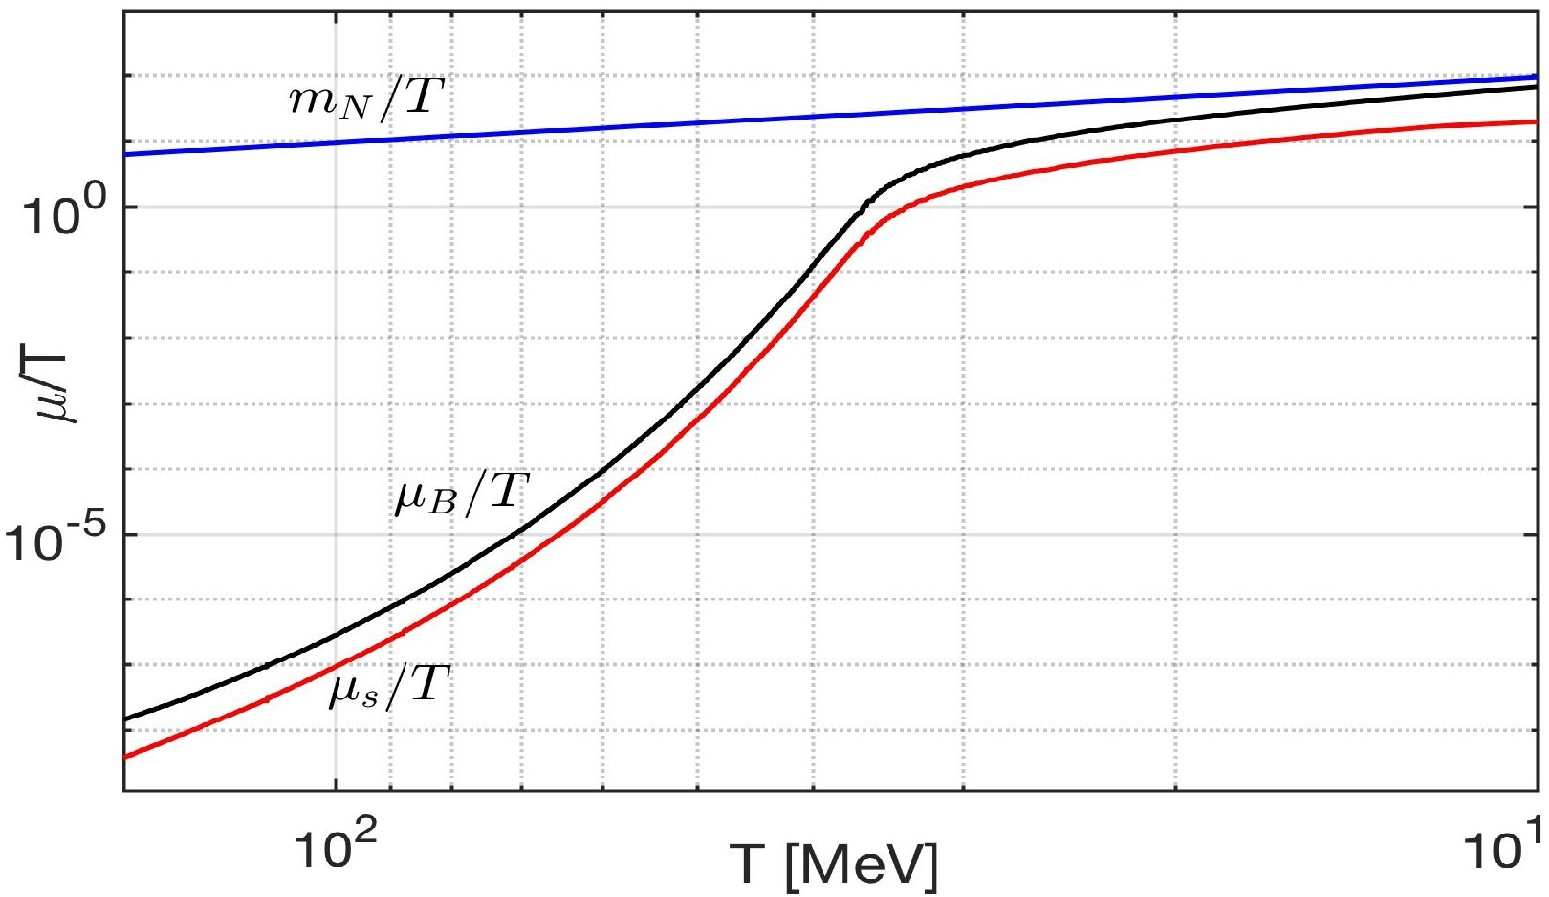
\includegraphics[width=0.8\linewidth]{./plots/New_Chemical_Potential_C.jpg}
\caption{The chemical potential of baryon $\mu_B/T$ and strangeness $\mu_s/T$ as a function of temperature $150\,\mathrm{MeV}> T>10\,\mathrm{MeV}$ in the early Universe; for comparison we show $m_N/T $ with $m_N=938.92$\,MeV, the average nucleon mass.}
\label{ChemPotFig}
%\end{center}
\end{figure}
%~~~~~~~~~~~~~~~~~~~~~~~~~~~~~~~~~~~~~~~~~~~~~~~~~~~~~~~~~~~~~~~~~~~~~~~~~~~~~~
%%%%%%%%%%%%%%%%%%%%%%%%%%%%%%%%%%%%%%%
\begin{figure}[h]
\centering
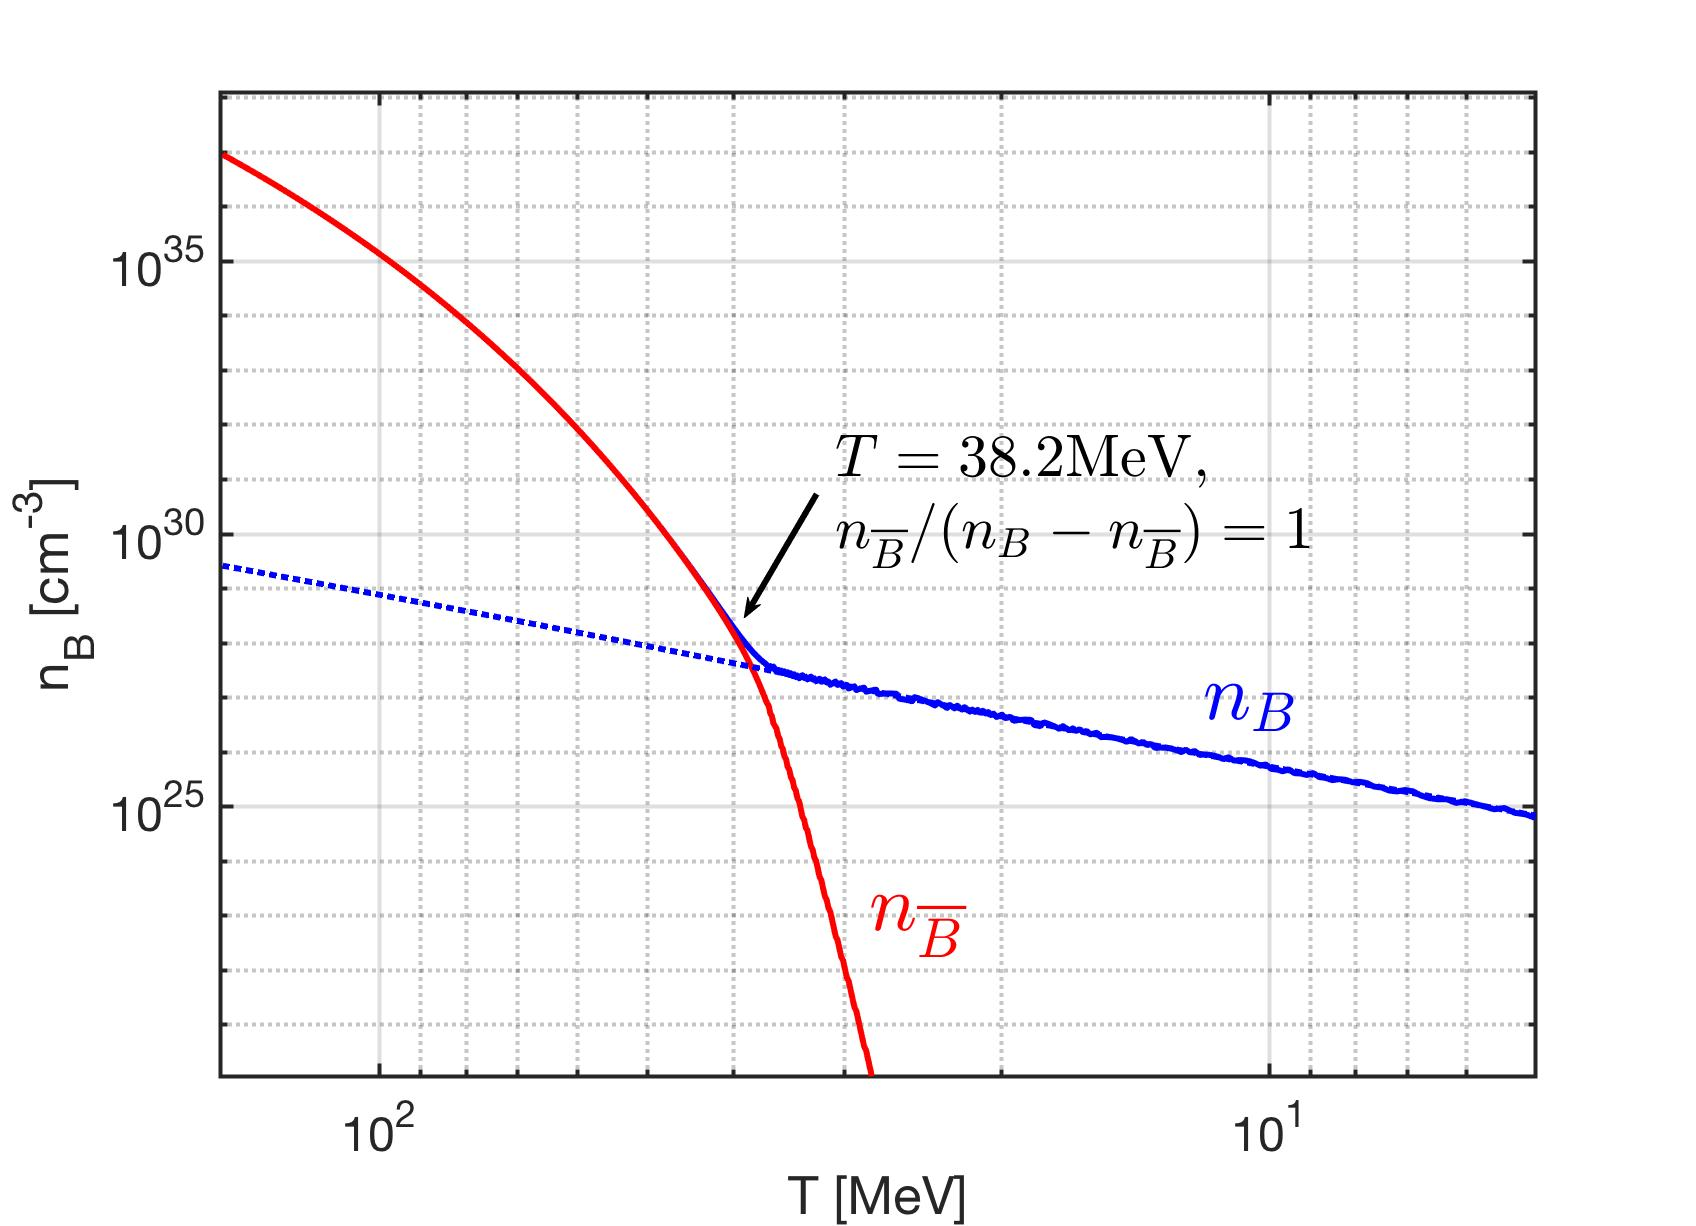
\includegraphics[width=\textwidth]{./plots/Baryon_Antibaryon_cm.jpg}
\caption{The baryon (blue solid line) and antibaryon (red solid line) number density as a function of temperature in the range $150\,\mathrm{MeV}>T>5\,\mathrm{MeV}$. The green dashed line is the extrapolated value for baryon density. The temperature $T=38.2\,\mathrm{MeV}$ (black dashed vertical line) is denoted when the ratio $n_{\overline B}/(n_B-n_{\overline B})=1$ which defines the condition where antibaryons disappear from the Universe.}
\label{Baryon_fig}
\end{figure}
%%%%%%%%%%%%%%%%%%%%%%%%%%%%%%%%%%%%%%%


We solve Eq.~(\,\ref{museq}) and Eq~(\ref{muBeq}) numerically to obtain baryon and strangeness chemical potentials as a function of temperature in Fig.~\ref{ChemPotFig}. The chemical potential changes dramatically in the temperature window $50\,\mathrm{MeV}\le T\le 30$\,MeV, its behavior describing the process of antibaryon disappearance. Substituting the chemical potential $\lambda_q$ and $\lambda_s$ into particle density Eq.~(\ref{Density_N}), Eq.~(\ref{Density_K}), and Eq.~(\ref{Density_Y}), we can obtain the particle number densities for different species as a function of temperature.

In Fig.~\ref{Baryon_fig} we plot the number density of baryon and antibaryon as a function of temperature. We consider that when the  $n_{\overline B}\ll(n_B-n_{\overline B})$ the anitbaryons density is sufficient low and disappear from the Universe inventory quickly. To determine the temperature where antibaryons is sufficient law in the Universe inventory we defined the condition when the ratio $n_{\overline B}/(n_B-n_{\overline B})=1$. This condition is reached in an expanding Universe at $T=38.2$\,MeV, which is in agreement with the qualitative result in [\cite{kolb1990early}]. After this temperature, the net baryon density dilutes with a residual co-moving conserved quantity determined by the observed baryon asymmetry.



%~~~~~~~~~~~~~~~~~~~~~~~~~~~~~~~~~~~~~~~~~~~~~~~~~~~~~~~~~~~~~~~~~~~~~~~~~~~~~~~~
\begin{figure}[bt]
%\begin{center}
\centering
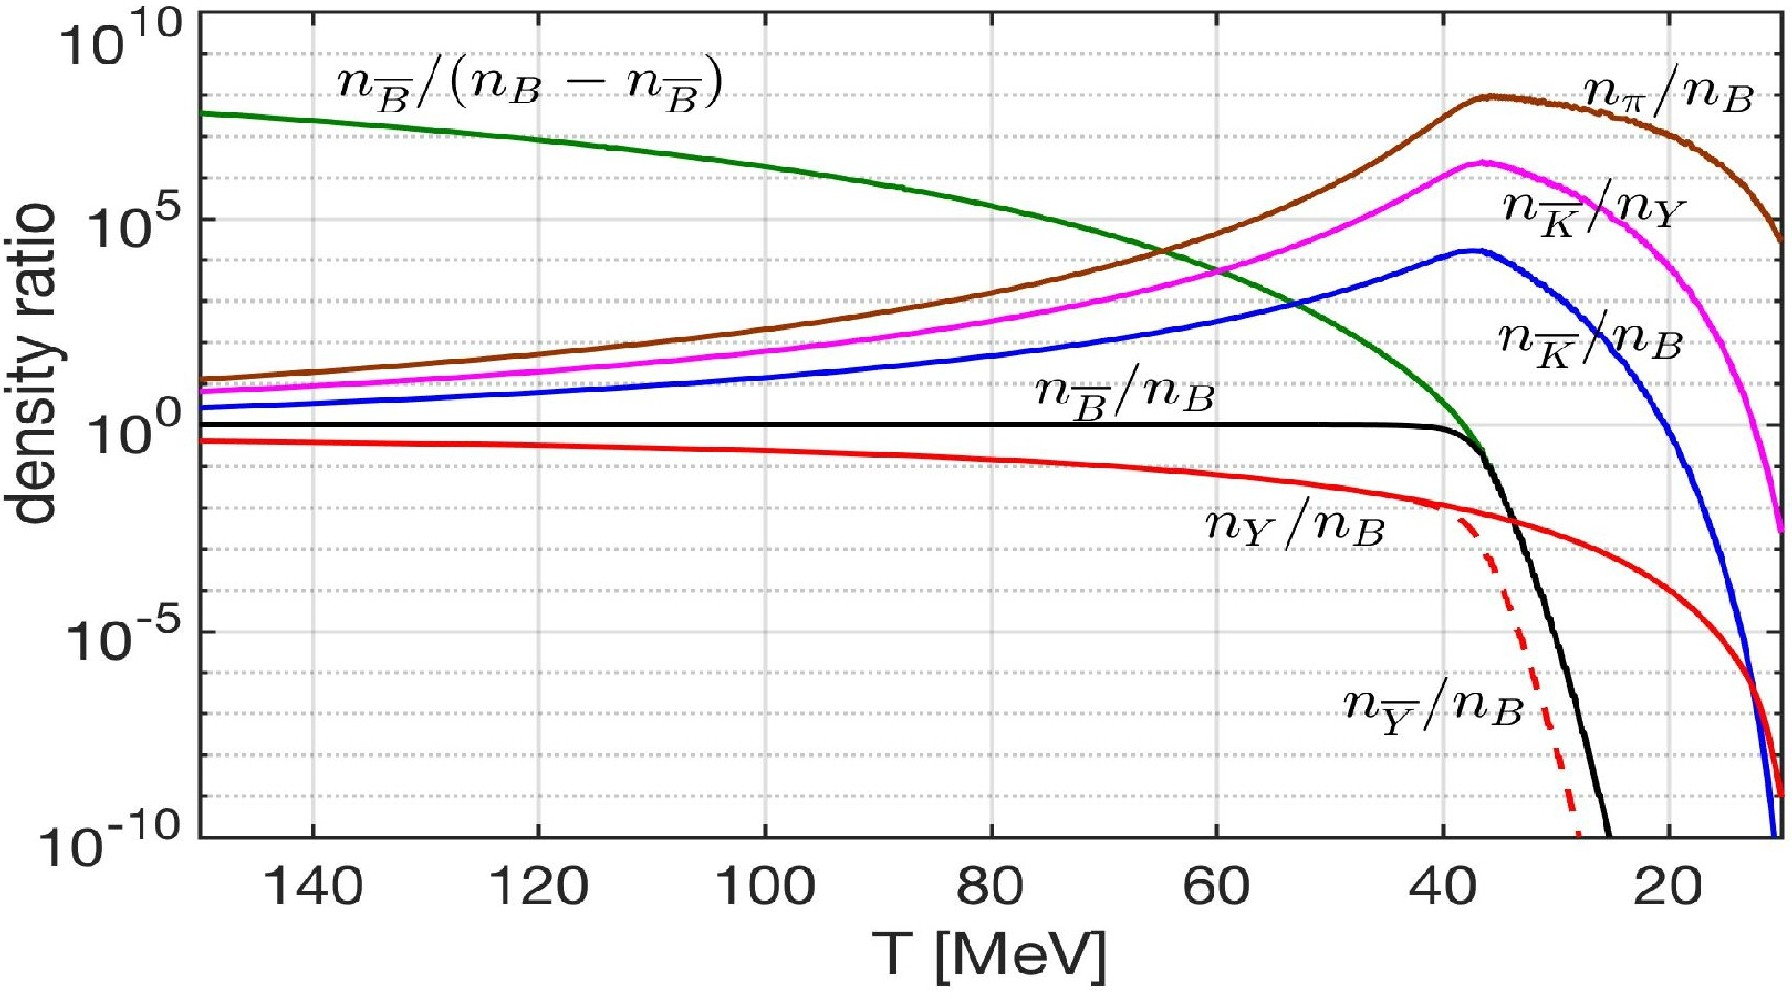
\includegraphics[width=0.85\linewidth]{./plots/Meson_Baryon_density_ratio_C.jpg}
\caption{Ratios of hadronic particle number densities as a function of temperature $150\,\mathrm{MeV}> T>10\,\mathrm{MeV}$ in the early Universe, with baryon $B$ yields: pions $\pi$ (brown line), kaons $K( q\bar s)$ (blue), antibaryon $\overline B$ (black), hyperon $Y$ (red) and anti-hyperons $\overline Y$ (dashed red). Also shown $\overline K/Y$(purple).}
\label{EquilibPartRatiosFig}
%\end{center}
\end{figure}
%~~~~~~~~~~~~~~~~~~~~~~~~~~~~~~~~~~~~~~~~~~~~~~~~~~~~~~~~~~~~~~~~~~~~~~~~~~~~~~

In Fig.~\ref{EquilibPartRatiosFig} we show examples of particle abundance ratios of interest. %Considering $n_Y/n_B$ we see that hyperons $Y(sqq)$ remain a noticeable 1\% component in baryon yield through this domain of antibaryon decoupling.
Pions $\pi(q\bar q)$ are the most abundant hadrons $n_\pi/n_B\gg1$, because of their low mass and the reaction $\gamma\gamma\rightarrow\pi^0$, which assures chemical yield equilibrium~[\cite{Kuznetsova:2008jt}]. For $150\,\mathrm{MeV}>T>20.8\,\mathrm{MeV}$, we see the ratio $n_{{\overline K}(\bar q s)}/n_B\gg1$, which implies pair abundance of strangeness is more abundant than baryons, and is dominantly present in mesons, since $n_{\overline K}/n_Y\gg1$. 
For $20.8\,\mathrm{MeV}>T$, the baryon becomes dominant $n_{\overline K}/n_B<1$, which implies that the strange meson is embedded in a large background of baryons, and the exchange reaction $\overline{K}+N\rightarrow \Lambda+\pi$ can re-equilibrate kaons and hyperons in the temperature range; therefore strangeness symmetry $s=\bar s$ is maintained. For $12.9\,\mathrm{MeV}>T$ we have $n_Y/n_B>n_{\overline K}/n_B$, now the still existent tiny abundance of strangeness is found predominantly in hyperons.


%~~~~~~~~~~~~~~~~~~~~~~~~~~~~~~~~~~~~~~~~~~~~~~~~~


\section{Seeking strangeness freeze-out chemical nonequilibrium
}
%In this section we will focus on the following:
%\begin{itemize}
%    \item Relevant strangeness reactions
%    \item Strangeness creation/annihilation in mesons
%    \item Strangeness production/ exchange in hyperons
%    \item Strangeness epochs in  the Universe 
%\end{itemize}

%In this section, we focus on investigating the strangeness abundance and decoupling following the formation of normal matter during the hadronization process of the quark-gluon plasma (QGP). Nonequilibrium conditions in the early Universe are of general interest: they are understood to be prerequisite for the arrow of time dependent processes to take hold in the Hubble expanding Universe.
%~~~~~~~~~~~~~~~~~~~~~~~~~~~~~~~~~~~~~~~~~~~~~~~~~~~~~~~~~~~~

%\subsection{Relevant strangeness reactions}
This section considers an unstable strange particle $S$ decaying into two particles $1$ and $2$, which themselves have no strangeness content. In a dense and high-temperature plasma with particles $1$ and $2$ in thermal equilibrium, the inverse reaction populates the system with particle $S$. This is written schematically as
\begin{align}
 S\Longleftrightarrow1+2,\qquad \mathrm{Example}: K^0\Longleftrightarrow\pi+\pi\,.
\end{align}
The natural decay of the daughter particles provides the intrinsic strength of the inverse strangeness production reaction rate. As long as both decay and production reactions are possible, particle $S$ abundance remains in thermal equilibrium. This balance between production and decay rates is called a detailed balance.

Once the primordial Universe expansion rate $1/H$ overwhelms the strongly temperature dependent back-reaction and the back reaction freeze-out, then the decay $S\rightarrow 1+2$ occurs out of balance and particle $S$ disappears from the inventory. The two-on-two strangeness producing reactions have a significantly higher strangeness production reaction threshold, thus especially near to strangeness decoupling their influence is negligible. Such reactions are more important near the QGP hadronization temperature $T_H\simeq 150$\,MeV, and they characterize strangeness exchange reactions such as $\mathrm{K}+N\leftrightarrow \Lambda+\pi$, (see Chapter 18 in [\cite{Letessier:2002ony}]).


In Fig.~\ref{Strangeness_map2} we show reactions relevant to strangeness evolution in the considered Universe evolution epoch $150\,\mathrm{MeV}\ge T\ge 10$\,MeV  and their pertinent reaction strength. As shown:
\begin{itemize}
\item
We study strange quark abundance in baryons and mesons, considering both open and hidden strangeness (hidden: $s\bar s$-content). Important source reactions are $l^-+l^+\rightarrow\phi$, $\rho+\pi\rightarrow\phi$, $\pi+\pi\rightarrow K_\mathrm{S}$, $\Lambda \leftrightarrow \pi+ N$, and $\mu^\pm+\nu\rightarrow K^\pm$. 
\item
Muons and pions are coupled through electromagnetic reactions $\mu^++\mu^-\leftrightarrow\gamma+\gamma$ and $\pi\leftrightarrow\gamma+\gamma$ to the photon background and retain their chemical equilibrium until the temperature $T =4$\, MeV and $T=5$\,MeV, respectively~[\cite{Rafelski:2021aey,Kuznetsova:2008jt}]. The large $\phi\leftrightarrow K+K$ rate assures $\phi$ and $K$ are in relative chemical equilibrium.
\end{itemize}
In order to determine where exactly strangeness disappears from the Universe inventory, we explore the magnitudes of different rates of production and decay processes in mesons and hyperons.
%~~~~~~~Figure~~~~~~~~~~~~~~~~~~~~~~~~~~~~~~~~~~~~~~~~~~~~~~~~~~~~~~~~~~~~~~~~~~~~
\begin{figure} %[h]
%\begin{center}
\centering
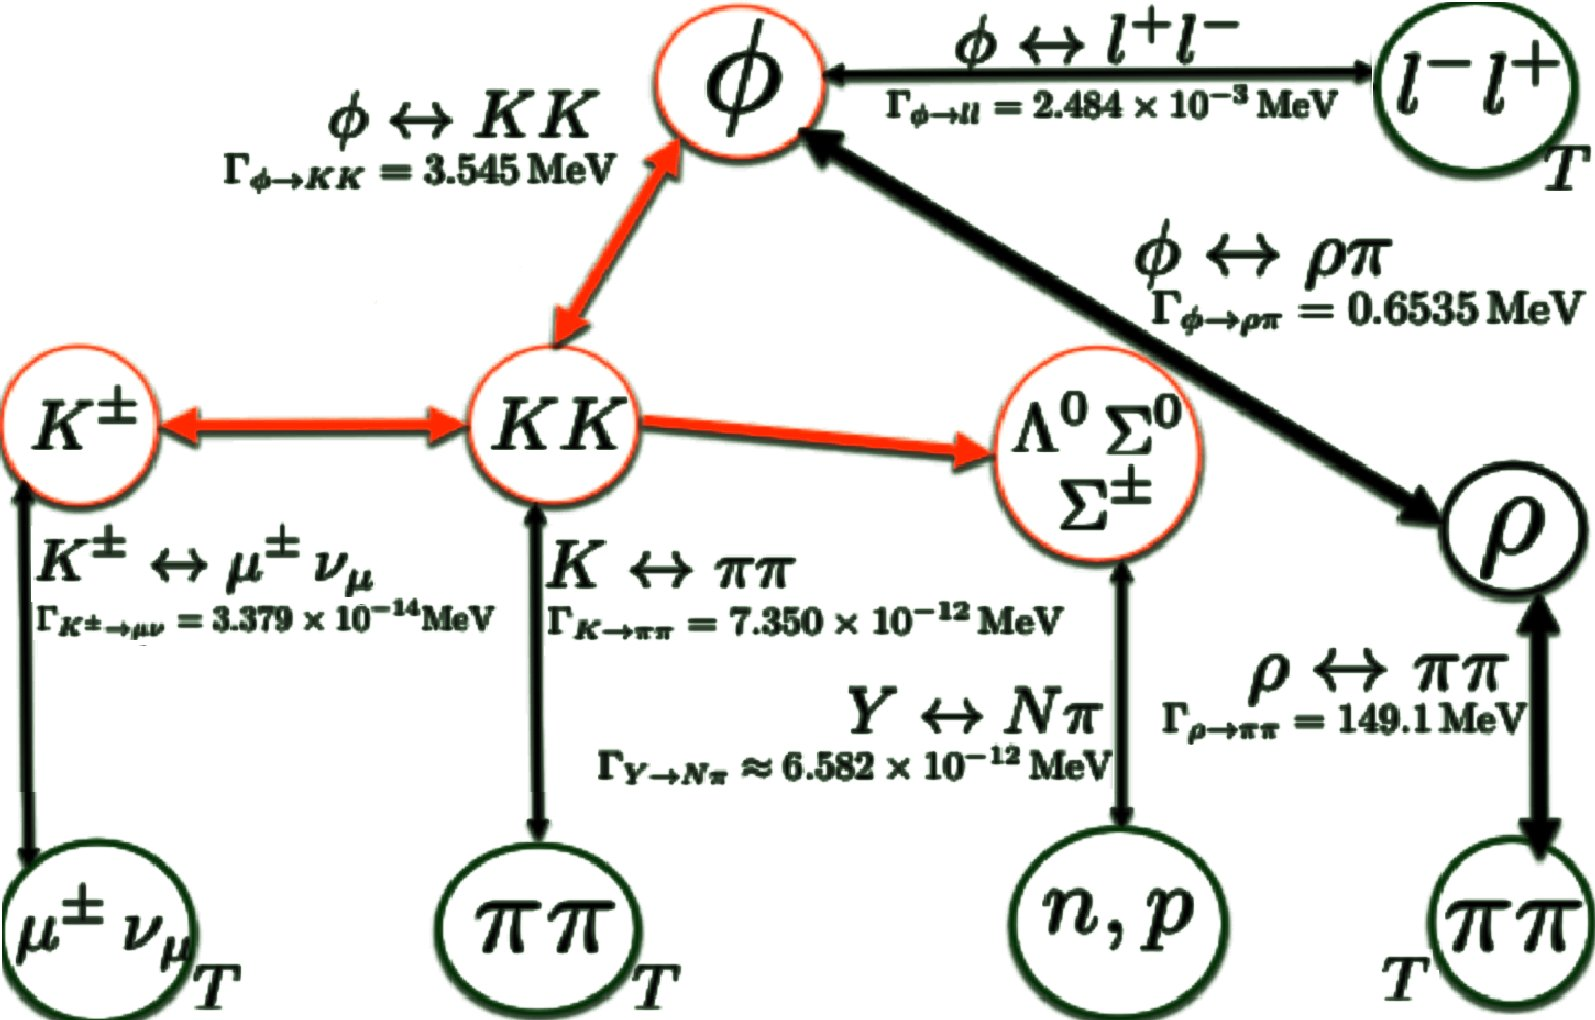
\includegraphics[width=0.75\linewidth]{./plots/Strangeness002_newJ.jpg}
\caption{
The strangeness abundance changing reactions in the primordial Universe. The red circles show strangeness carrying hadronic particles; red thick lines denote effectively instantaneous reactions. Black thick lines show relatively strong hadronic reactions. The reaction rates required to describe  strangeness time evolution are shown in [\cite{Rafelski:2020ajx}].
}
\label{Strangeness_map2}
%\end{center}
\end{figure}
%~~~~~~~~~~~~~~~~~~~~~~~~~~~~~~~~~~~~~~~~~~~~~~~~~~~~~~~~~~~~~~~~~~~~~~~~~~



\subsection{Strangeness creation/annihilation rate in mesons}
From Fig.~\ref{Strangeness_map2} in the meson domain, the relevant interaction rates competing with Hubble time are the reactions
\begin{align}
 &\pi+\pi\leftrightarrow K\,,\quad\mu^\pm+\nu\leftrightarrow K^\pm\,,\quad l^++l^-\leftrightarrow\phi\,,\\
 &\rho+\pi\leftrightarrow\phi\,,\quad \pi+\pi\leftrightarrow\rho\,.
\end{align}
The thermal reaction rate per time and volume for two body-to-one particle reactions $1+2\rightarrow 3$ has been presented before~[\cite{Koch:1986ud,Kuznetsova:2008jt,Kuznetsova:2010pi}]. In full kinetic and chemical equilibrium, the reaction rate per time per volume can be written as~[\cite{Kuznetsova:2010pi}] :
\begin{align}
&R_{12\to 3}=\frac{g_3}{(2\pi)^2}\,\frac{m_3}{\tau^0_3}\,\int^\infty_0\frac{p^2_3dp_3}{E_3}\frac{e^{E_3/T}}{e^{E_3/T}\pm1}\Phi(p_3)\;,
\end{align}
where $\tau^0_3$ is the vacuum lifetime of particle $3$. The positive sign $``+"$ is for the case when particle $3$ is a boson, and negative sign $``-"$ for fermion. The function $\Phi(p_3)$ for the non-relativistic limit $m_3\gg p_3,T$ can be written as 
\begin{align}
\Phi(p_3\to0)=2\frac{1}{(e^{E_1/T}\pm1)(e^{E_2/T}\pm1)}.
\end{align}


Considering the Boltzmann limit, the thermal reaction rate per unit time and volume becomes
\begin{align}
\label{Thermal_Rate}
R_{12\rightarrow3}=\frac{g_3}{2\pi^2}\left(\frac{T^3}{\tau^0_3}\right)\left(\frac{m_3}{T}\right)^2\,K_1(m_3/T),
\end{align}
where $K_1$ is the modified Bessel functions of integer order "$1$". In order to compare the reaction time with Hubble time $1/H$, it is convenient to define the relaxation time for the process $1+2\rightarrow 3$ as follows:
\begin{align}
\label{Reaction_Time}
\tau_{12\rightarrow 3}\equiv\frac{n^{eq}_{1}}{R_{12\rightarrow n}}\,,\quad
n^{eq}_1=\frac{g_1}{2\pi^2}\int_{m_1}^\infty\!\!\!\!dE\,\frac{E\,\sqrt{E^2-m_1^2}}{\exp{\left(E/T\right)}\pm1}\;, 
\end{align}
where $n^{eq}_1$\,is the thermal equilibrium number density of particle\,$1$ with the `heavy' mass $m_1>T$.  Combining Eq.\,(\ref{Thermal_Rate}) with  Eq.\,(\ref{Reaction_Time}) we obtain
\begin{align}\label{RelaxationTime}
&\frac{\tau_{12\rightarrow3}}{ \tau^0_3}=  
\frac{2\pi^2 n^{eq}_1/T^3}{g_3(m_3/T)^2\,K_1(m_3/T)}\,, \quad 
n^{eq}_1\simeq g_1\left(\frac{m_1 T}{2\pi}\right)^{3/2}e^{-m_1/T},
\end{align}
where, conveniently, the relaxation time does not depend on the abundant and often relativistic heat bath component $2$, {\it e.g.\/} $l^\pm,\pi,\nu,\gamma$. The density of heavy particles\,$1$\,and\,$3$ can in general be well approximated using the leading and usually nonrelativistic Boltzmann term as shown above.

In general, the reaction rates for inelastic collision process capable of changing particle number, for example $\pi\pi\to K^0$, is suppressed by the factor $\exp{(-m_{K^0}/T)}$. On the other hand, there is no suppression for the elastic momentum and energy exchanging particle collisions in plasma. We conclude that for the case $m\gg T$, the dominant collision term in the relativistic Boltzmann equation is the elastic collision term, keeping all heavy particles in kinetic energy equilibrium with the plasma. This allows us to study the particle abundance in plasma presuming the energy-momentum statistical distribution equilibrium exists. This insight was discussed in detail in the preparatory phase of laboratory exploration of hot hadron and quark matter, see~[\cite{Koch:1986ud}]. In order to study the particle abundance in the Universe when $m\gg T$, instead of solving the exact Boltzmann equation, we can separate the fast energy-momentum equilibrating collisions from the slow particle number changing inelastic collisions. In the following we explore the rates of inelastic collision and compare the relaxation times of particle production in all relevant reactions with the Universe expansion rate.



It is common to refer to particle freeze-out as the epoch where a given type of particle ceases to interact with other particles. In this situation the particle abundance decouples from the cosmic plasma, a chemical nonequilibrium and even complete abundance disappearance of this particle can happen; the condition for the given reaction $1+2\rightarrow 3$ to decouple is
\begin{align}
\tau_{12\rightarrow 3}(T_f)=1/H(T_f),
\end{align}
where $T_f$ is the freeze-out temperature.
In the epoch of interest, $150\,\mathrm{MeV}>T>10\,\mathrm{MeV}$, the Universe is dominated by radiation and effectively massless matter behaving like radiation. The Hubble parameter can be written as~[\cite{Kolb:1990vq}]
\begin{align}\label{H2g}
H^2=H^2_{rad}\left(1+\frac{\rho_{\pi,\,\mu,\,\rho}}{\rho_\mathrm{rad}}+\frac{\rho_\mathrm{strange}}{\rho_\mathrm{rad}}\right)=\frac{8\pi^3G_\mathrm{N}}{90}g^e_\ast T^4,\qquad H^2_\mathrm{rad}=\frac{8\pi G_\mathrm{N}\,\rho_\mathrm{rad}}{3},
\end{align}
where: $g^e_\ast$ is the total number of effective relativistic `energy' degrees of freedom; $G_\mathrm{N}$ is the Newtonian constant of gravitation; the `radiation' energy density includes $\rho_\mathrm{rad}=\rho_\gamma+\rho_\nu+\rho_{e^\pm}$ for photons, neutrinos, and massless electrons(positrons). The massive-particle correction is $\rho_{\pi,\,\mu,\,\rho}=\rho_\pi+\rho_\mu+\rho_\rho$; and at highest $T$ of interest, also of (minor) relevance, $\rho_\mathrm{strange}=\rho_{K^0}+\rho_{K^\pm}+\rho_{K^\ast}+\rho_{\eta}+\rho_{\eta^\prime}$.
%~~~~~~~Figure~~~~~~~~~~~~~~~~~~~~~~~~~~~~~~~~~~~~~~~~~~~~~~~~~~~~~~~~~~~~~~~~~~~~~~~~~~
\begin{figure}[ht]
%\begin{center}
\centering
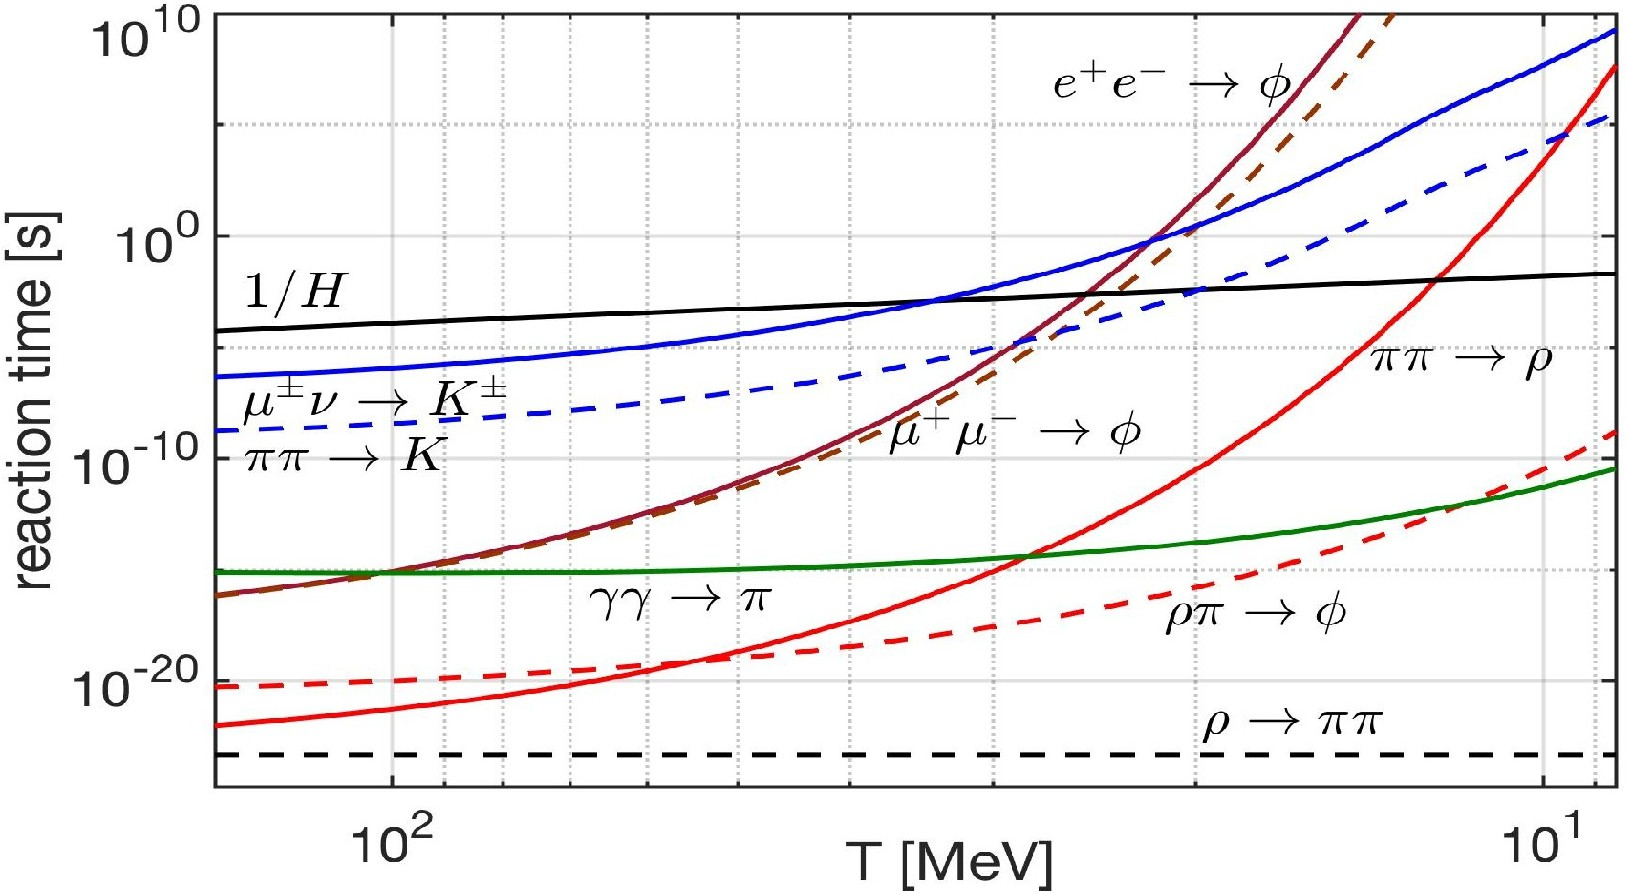
\includegraphics[width=0.95\linewidth]{./plots/Strangeness_Hubble_C.jpg}
\caption{Hadronic relaxation reaction times, see Eq.\,(\ref{Reaction_Time}), as a function of temperature $T$, are compared to Hubble time $1/H$ (black solid line). At bottom the horizontal black-dashed line is the natural (vacuum) lifespan of $\rho$.}
\label{reaction_time_tot}
%\end{center}
\end{figure}
%~~~~~~~~~~~~~~~~~~~~~~~~~~~~~~~~~~~~~~~~~~~~~~~~~~~~~~~~~~~~~~~~~~~~~~~~~~~~~~~~~~~~~


When presenting the reaction rates and quoting decoupling as a function of temperature $T$, we must remember that for a temperature range $50\,\mathrm{MeV}>T>5$\,MeV, we have $10^{-1}<dT/dt<10^{-4}$\,MeV/$\mu$s. We estimate the width of freezeout temperature interval $\Delta T_f$  as follows:
\begin{align}
\frac{1}{\Delta T_f}\equiv \left[\frac{1}{(\Gamma_{12\to3}/H)}\frac{d(\Gamma_{12\to3}/H)}{dT}\right]_{T_f},\quad \Gamma_{12\to3}\equiv\frac{1}{\tau_{12\to3}}.
\end{align}
Using Eq.(\ref{H2g}) and Eq.(\ref{RelaxationTime}) and considering the temperature range $50\,\mathrm{MeV}>T>5$\,MeV with $g^e_\ast\approx\mathrm{constant}$ we obtain using the Boltzmann approximation to describe the  massive particles\,$1$\,and\,$3$
\begin{align}\label{DeltaFreezeout}
 \frac{\Delta T_f}{ T_f} \approx\frac{T_f  }{ m_3 - m_1 -2T_f}\,,\quad m_3 - m_1>> T_f\,.
\end{align}
The width of freeze-out is shown in the right column in Table~\ref{FreezeoutTemperature_table}. We see a range of $2$-$10\%$. Therefore it is justified to consider as a decoupling condition in time the value of temperature at which the pertinent rate cross the Hubble expansion rate, see Fig.~\ref{reaction_time_tot}.
 
In Fig.~\ref{reaction_time_tot} we plot the  hadronic reaction relaxation times $\tau_{i}$ in the meson sector as a function of temperature compared to Hubble time $1/H$.
It shows that the weak interaction reaction $\mu^\pm+\nu_{\mu}\rightarrow K^\pm$ becomes slower compared to the Universe expansion near temperature $T_f^{K^\pm}=33.8\,\mathrm{MeV}$, signaling the onset of abundance nonequilibrium for $K^\pm$. For $T<T_f^{K^\pm}$, the reactions $\mu^\pm+\nu_{\mu}\rightarrow K^\pm$ decouples from the cosmic plasma; the corresponding detailed balance can be broken and the decay reactions $K^\pm\rightarrow\mu^\pm+\nu_{\mu}$ are acting like a (small) ``hole'' in the strangeness abundance ``pot''. If other strangeness production reactions did not exist, strangeness would disappear as the Universe cools below $T_f^{K^\pm}$. However, we have other reactions: $l^++l^-\leftrightarrow\phi$, $\pi+\pi\leftrightarrow K$, and $\rho+\pi\leftrightarrow\phi$ can still produce the strangeness in cosmic plasma and the rate is very large compared to the weak interaction decay.
%~~~~~~~~~~~~~~~~~~~~~~~~~~~~~~~~~~~~~~~~~~~~~~~~~~~~~~~~~~~~~~~~~~~~~~~~~~~~~~~~~~~~~~~~~
\begin{table}%[h]
\centering
\begin{tabular}{c| c| c}
\hline\hline
Reactions &Freeze-out Temperature (MeV) & {$\Delta T_f$\,(MeV)} \\
\hline
$\mu^\pm\nu\rightarrow K^\pm$ & $T_f=33.8$\,MeV & {$3.5$ \,MeV}\\ 
\hline
$e^+e^-\rightarrow \phi$ & $T_f=24.9$\,MeV &{$0.6$\,MeV}\\
$\mu^+\mu^-\rightarrow\phi$ & $T_f=23.5$\,MeV &{$0.6$\,MeV}\\
\hline
 $\pi\pi\rightarrow K$ & $T_f=19.8$\,MeV&{$1.2$\,MeV}\\
\hline
$\pi\pi\rightarrow\rho$ & $T_f=12.3$\,MeV&{$0.2$\,MeV}\\
\hline\hline
\end{tabular}
\caption{The characteristic strangeness reaction and their freeze-out temperature and temperature width in early Universe.}
\label{FreezeoutTemperature_table} 
\end{table}

%~~~~~~~~~~~~~~~~~~~~~~~~~~~~~~~~~~~~~~~~~~~~~~~~~~~~~~~~~~~~~~~~~~~~~~~~~ 

In Table~\ref{FreezeoutTemperature_table} we show the characteristic strangeness reactions and their freeze-out temperatures in the early Universe. The intersection of strangeness reaction times with $1/H$ occurs for $l^-+l^+\rightarrow\phi$ at $T_f^\phi=25\sim23\,\mathrm{MeV}$, and for $\pi+\pi\rightarrow K$ at $T_f^K=19.8\,\mathrm{MeV}$, for $\pi+\pi\rightarrow\rho$ at $T_f^\rho=12.3\,\mathrm{MeV}$. The reactions $\gamma+\gamma\rightarrow\pi$ and $\rho+\pi\leftrightarrow\phi$ are faster compared to $1/H$. However, the $\rho\to\pi+\pi$ lifetime (black dashed line in Fig.~\ref{reaction_time_tot}) is smaller than the reaction $\rho+\pi\leftrightarrow\phi$; in this case, most of $\rho$-meson decays faster, thus are absent and cannot contribute to the strangeness creation in the meson sector. Below the temperature $T<20$\,MeV, all the detail balances in the strange meson reactions are broken and the strangeness in the meson sector should disappear rapidly, were it not for the small number of baryons present in the Universe.



%~~~~~~~~~~~~~~~~~~~~~~~~~~~~~~~~~~~~~~~~~~~~~~~~~~~~~~~~



\subsection{Strangeness production/ exchange rate in hyperons}
In order to understand strangeness in hyperons in the baryonic domain, we now consider the strangeness production reaction $\pi +N\rightarrow K+\Lambda$, the strangeness exchange reaction $\overline{K}+N\rightarrow \Lambda+\pi$; and the strangeness decay $\Lambda\rightarrow N+\pi$. The competition between different strangeness reactions allows strange hyperons and antihyperons to influence the dynamic nonequilibrium condition, including development of $\langle s-\bar s\rangle \ne 0$. %The cross sections $\sigma_{\overline{K}N\rightarrow \Lambda\pi}$ and $\sigma_{\pi N\rightarrow K\Lambda}$ are obtained from experiment.

To evaluate the reaction rate in two-body reaction $1+2\rightarrow3+4$ in the Boltzmann approximation we can use the reaction cross section $\sigma(s)$ and the relation~[\cite{Letessier:2002ony}]:
\begin{align}
R_{12\rightarrow34}=\frac{g_1g_2}{32\pi^4}\frac{T}{1+I_{12}}\!\!\int^\infty_{s_{th}}\!\!\!\!ds\,\sigma(s)\frac{\lambda_2(s)}{\sqrt{s}}\!K_1\!\!\left({\sqrt{s}}/{T}\right),
\end{align}
where $K_1$ is the Bessel function of order $1$ and the function $\lambda_2(s)$ is defined as
\begin{align}
\lambda_2(s)=\left[s-(m_1+m_2)^2\right]\left[s-(m_1-m_2)^2\right],
\end{align}
with $m_1$ and $m_2$, $g_1$ and $g_2$ as the masses and degeneracy of the initial interacting particle. The factor $1/(1+I_{12})$ is introduced to avoid double counting of indistinguishable pairs of particles; we have $I_{12}=1$ for identical particles and $I_{12}=0$ for others. 

The thermal averaged cross sections for the strangeness production and exchange processes are about $\sigma_{\pi N\rightarrow K\Lambda}\sim0.1\,\mathrm{mb}$ and $\sigma_{\overline{K}N\rightarrow \Lambda\pi}=1\sim3\,\mathrm{mb}$ in the energy range in which we are interested~[\cite{Koch:1986ud}]. The cross section can be parameterized as follows:\\
1) For the cross section $\sigma_{\overline{K}N\rightarrow \Lambda\pi}$ we use~[\cite{Koch:1986ud}]
 \begin{align}
 \sigma_{\overline{K}N\rightarrow \Lambda\pi}=\frac{1}{2}\left(\sigma_{K^-p\rightarrow \Lambda\pi^0}+\sigma_{K^-n\rightarrow \Lambda\pi^-}\right)\,.
\end{align}
Here the experimental cross sections can be parameterized as 
\begin{align}
&\sigma_{K^-p\rightarrow \Lambda\pi^0}\!\!=\!\!\left(\begin{array}{l}\!\!1479.53\mathrm{mb}\!\cdot\!\exp{\left(\frac{-3.377\sqrt{s}}{\mathrm{GeV}}\right)},\; \mathrm{for}\,\sqrt{s_m}\!\!<\!\!\sqrt{s}\!<\!3.2\mathrm{GeV} \\ \\0.3\mathrm{mb}\!\cdot\!\exp{\left(\frac{-0.72\sqrt{s}}{\mathrm{GeV}}\right)},\; \mathrm{for}\sqrt{s}>3.2\mathrm{GeV}\end{array}\right.\\
&\sigma_{K^-n\rightarrow \Lambda\pi^-}\!\!=\!\!1132.27\mathrm{mb}\!\cdot\!\exp{\left(\frac{-3.063\sqrt{s}}{\mathrm{GeV}}\right)},\; \mathrm{for}\sqrt{s}>1.699\mathrm{GeV},
\end{align}
where $\sqrt{s_m}=1.473$ GeV.\\
2) For the cross section $\sigma_{\pi N\rightarrow K\Lambda}$ we use~[\cite{Cugnon:1984pm}]
\begin{align}
&\sigma_{\pi N\rightarrow K\Lambda}=\frac{1}{4}\times\sigma_{\pi p\rightarrow K^0\Lambda}\,.
\end{align}
The experimental $\sigma_{\pi p\rightarrow K^0\Lambda}$  can be approximated as follows
\begin{align}
\sigma_{\pi p\rightarrow K^0\Lambda}=\left(\begin{array}{l}\frac{0.9\mathrm{mb}\cdot\left(\sqrt{s}-\sqrt{s_0}\right)}{0.091\mathrm{GeV}},\; \mathrm{for} \sqrt{s_0}<\sqrt{s}<1.7\mathrm{GeV} \\ \\ \frac{90\mathrm{MeV\cdot mb}}{\sqrt{s}-1.6\mathrm{GeV}},\; \mathrm{for}\sqrt{s}>1.7\mathrm{GeV},\end{array}\right.
 \end{align}
 with $ \sqrt{s_0}=m_\Lambda+m_K$. 


Given the cross sections, we obtain the thermal reaction rate per volume for strangeness exchange reaction seen in Fig.~\ref{Lambda_Rate_volume.fig}. We see that around $T=20$\,MeV, the dominant reactions for the hyperon $\Lambda$ production is $\overline{K}+N\leftrightarrow\Lambda+\pi$. At the same time, the $\pi+\pi\to K$ reaction becomes slower than Hubble time and kaon $K$ decay rapidly in the early Universe. However, the anti-kaons $\overline K$ produce the hyperon $\Lambda$ because of the strangeness exchange reaction $\overline{K}+N\rightarrow\Lambda+\pi$ in the baryon-dominated Universe. We have strangeness in $\Lambda$ and it disappears from the Universe via the decay $\Lambda\rightarrow N+\pi$. Both strangeness and anti-strangeness disappear because of the $K\rightarrow\pi+\pi$ and $\Lambda\rightarrow N+\pi$, while the strangeness abundance $s = \bar{s}$ in the early Universe remains.

%~~~~~~~~~~~~~~~~~~~~~~~~~~~~~~~~~~~~~~~~~~~~~~~~~~~~~~~~~~~~~~~~~~~~~~~~~~~~~~~~
\begin{figure}[ht]
%\begin{center}
\centering
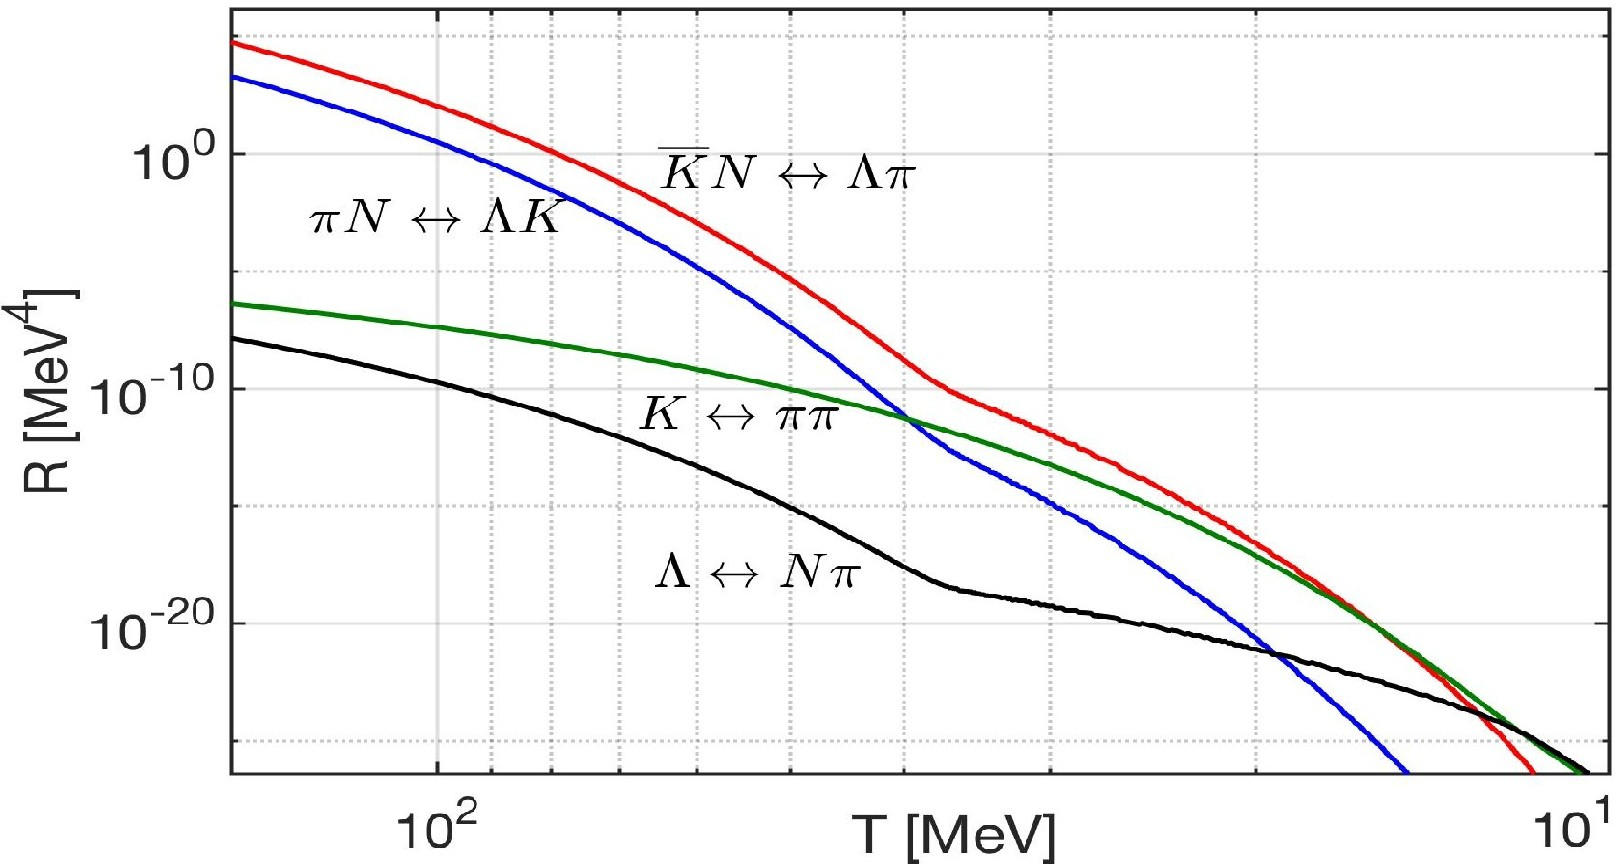
\includegraphics[width=0.9\linewidth]{./plots/NewHyperonRate_C.jpg}
\caption{Thermal reaction rate $R$ per volume and time for important hadronic strangeness production and exchange processes as a function of temperature $150\,\mathrm{MeV}> T>10\,\mathrm{MeV}$ in the early Universe.}
\label{Lambda_Rate_volume.fig}
%\end{center}
\end{figure}
%~~~~~~~~~~~~~~~~~~~~~~~~~~~~~~~~~~~~~~~~~~~~~~~~~~~~~~~~~~~~~~~~~~~~~~~~~~~~~~

Around $T=12.9$\,MeV, the reaction $\Lambda+\pi\rightarrow\overline{K}+N$ becomes slower than the strangeness decay $\Lambda\leftrightarrow N+\pi$ and shows that at the low temperature the $\Lambda$ particles are still in equilibrium via the reaction $\Lambda\leftrightarrow N+\pi$ and little strangeness remains in the $\Lambda$. Then strangeness abundance becomes asymmetric $s\gg \bar{s}$, which implies that the assumption for strangeness conservation can only be valid until the temperature $T\sim13$\,MeV. Below this temperature a new regime opens up in which the tiny residual strangeness abundance is governed by weak decays with no re-equilibration with mesons. Also, in view of baron asymmetry, $\langle s-\bar s\rangle \ne 0$.

The primary conclusion of this first study of strangeness production and content in the early Universe, following on QGP hadronization, is that the relevant temperature domains indicate a complex interplay between baryon and meson (strange and non-strange) abundances and non-trivial decoupling from equilibrium for strange and non-strange mesons. We believe that this work contributes to the opening of a new and rich domain in the study of the Universe evolution in the future. 

%~~~~~~~~~~~~~~~~~~~~~~~~~~~~~~~~~~~~~~~~~~~~~~~~~

%{Introduction\daggerfootnote{This chapter has been published previously as \citet{Gottbrath1999}.}}


\section{Neutrino Plasma}\label{Neutrino}
\subsection{Neutrino properties and reactions}\label{ssec:nuproperties}
Neutrinos are fundamental particles which play an important role in the evolution of the Universe. In the early Universe the neutrinos are kept in equilibrium with cosmic plasma via the weak interaction. The neutrino-matter interactions plays a crucial role in  understanding of neutrinos evolution in the early Universe (such as neutrino freeze-out) and the later Universe (the property of today's neutrino background). In this chapter, we will examine the neutrino coherent and incoherent scattering with matter and their application in cosmology. The investigation of the relation between the effective number of neutrinos\index{neutrino!effective number} $N^{\mathrm{eff}}_\nu$ and lepton asymmetry\index{lepton!asymmetry} $L$ after neutrino freeze-out\index{neutrino!freeze-out} and its impact on Universe expansion is also discussed in this chapter. 

%%%%%%%%%%%%%%%%%%%%%%%%%%%%%%
\para{Matrix elements for neutrino coherent \& incoherent scattering}
 According to the standard model, neutrinos interact with other particles via the Charged-Current(CC) and Neutral-Current(NC) interactions. Their Lagrangian can be written as~\cite{Giunti:2007ry}
\begin{align}
&\mathcal{L}^{CC}=\frac{g}{2\sqrt{2}}\left(j^\mu_W\,W_\mu+{j^\mu_W}^\dagger\,W^\dagger_\mu\right),\qquad\mathcal{L}^{NC}=-\frac{g}{2\cos{\theta_w}}\,j^\mu_Z\,Z_\mu,
\end{align}
where $g=e\sin\theta_w$, $W^\mu$ and $Z^\mu$ are W and Z boson gauge fields, and $j^\mu_W$ and $j^\mu_Z$ are the charged-current and neutral-current separately. In the limit of energies lower than the $W(m_w=80\,\mathrm{GeV})$ and $Z(m_z=91\,\mathrm{GeV})$ gauge bosons, the effective Lagrangians are given by
\begin{align}\label{L_low}
\mathcal{L}^{CC}_{eff}=-\frac{G_F}{\sqrt{2}}\,j^\dagger_{W\,\mu}\,j^\mu_W,\qquad
\mathcal{L}^{NC}_{eff}=-\frac{G_F}{\sqrt{2}}\,j^\dagger_{Z\,\mu}\,j^\mu_Z,\qquad \frac{G_F}{\sqrt{2}}=\frac{g^2}{8m^2_W},
\end{align}
where $G_F=1.1664\times10^{-5}\,\mathrm{GeV}^{-2}$ is the Fermi constant, which is one of the important parameters that determine the strength of the weak interaction rate. When neutrinos interact with matter, based on the neutrino's wavelength, they can undergo two types of scattering processes: coherent scattering and incoherent scattering with the particles in the medium. 

With coherent scattering, neutrinos interact with the entire  composite system rather than individual particles within the system. The coherent scattering is particularly relevant for low-energy neutrinos when the wavelength of neutrino is much larger than the size of system. In $1978$, Lincoln Wolfenstein pointed out that the coherent forward scattering of neutrinos off matter could be very important in studying the behavior of neutrino flavor oscillation\index{neutrino!flavor oscillation} in a dense medium~\cite{Wolfenstein:1977ue}. The fact that neutrinos propagating in matter may interact with the background particles can be described by the picture of free neutrinos traveling in an effective potential.

For incoherent scattering, neutrinos interact with particles in the medium individually. Incoherent scattering is typically more prominent for high-energy neutrinos, where the wavelength of neutrino is smaller compared to the spacing between particles. Study of incoherent scattering of high-energy neutrinos is important for understanding the physics in various astrophysical systems (e.g. supernova, stellar formation) and the evolution of the early Universe.

In this section, we discuss the coherent scattering between long wavelength neutrinos and atoms, and study the effective potential for neutrino coherent interaction. Then we present the matrix elements that describe the incoherent interaction between high energy neutrinos and other fundamental particles in the early Universe. Understanding these matrix elements is crucial for comprehending the process of neutrino freeze-out in the early Universe.

%%%%%%%%%%%%%%%%%%%%%%%%%%%%%%%%
\para{Long wavelength limit of neutrino-atom coherent scattering}
%\label{LongWavelength}
According to the standard cosmological model, the Universe today is filled with the cosmic neutrinos with temperature $T_{\nu}^0=1.9 \,\mathrm{K}=1.7\times10^{-4}\,\mathrm{eV}$. The average momentum of present-day relic neutrinos is given by $\langle p_\nu^0\rangle\approx3.15\,T_\nu^0$ and the typical wavelength $\lambda_{\nu}^{0}={2\pi}/{\langle p_{\nu}^{0}\rangle}\approx2.3\times10^5\,$\AA, which is much larger than the radius at the atomic scale, such as the Bohr radius $R_{\mathrm{atom}}=0.529\,$\AA. In this case we have the long wavelength condition $\lambda_\nu\gg\,R_{\mathrm{atom}}$ for cosmic neutrino background today.  

Under the condition $\lambda_\nu\gg\,R_{\mathrm{atom}}$, when the neutrino is scattering off an atom, the interaction can be coherent scattering~\cite{PhysRevD.38.32,Lewis:1979mu,Papavassiliou:2005cs}. According to the principles of quantum mechanics, with neutrino scattering it is impossible to identify which scatters the neutrino interacts with and thus it is necessary to sum over all possible contributions. In such circumstances, it is appropriate to view the scattering reaction as taking place on the atom as a whole, i.e.,\index{neutrino!coherent scattering}
\begin{align}
\nu+\mathrm{Atom}\longrightarrow\nu+\mathrm{Atom}.
\end{align}

Considering a neutrino elastic scattering off an atom which is composed of $Z$ protons, $N$ neutrons and $Z$ electrons. For the elastic neutrino atom scattering, the low-energy neutrinos scatter off both atomic electrons and nucleus. For nucleus parts, we consider that the neutrinos interact via the $Z^0$ boson with a nucleus as
\begin{align}
\nu+A^{Z}_N\longrightarrow\nu+A^{Z}_N.
\end{align}
In this process a neutrino of any flavor scatters off a nucleus with the same strength. Therefore, the scattering will be insensitive to neutrino flavor. On the other hand, the neutrons can also interact via the $W^\pm$ with nucleus as 
\begin{align}
\nu_l+A^{Z}_N\longrightarrow\,l^-+A^{{Z}+1}_N,
\end{align}
which is a quasi-elastic process for neutrino scattering with the nucleus; we have $A^{Z_e}_N\rightarrow\,A^{{Z_e}+1}_N$. Since this process will change the nucleus state into an excited one, we will not consider its effect here. For detail discussion pf quasi-elastic scattering see ~\cite{SajjadAthar:2022pjt}.

For atomic electrons, the neutrinos can interact via the $Z^0$ and $W^\pm$ bosons with electrons for different flavors, we have
\begin{align}
&\nu_e+e^-\longrightarrow\nu_e+e^-\,\,\,(\mathrm{Z^0,\,W^\pm\,exchange}),\\
&\nu_{\mu,\tau}+e^-\longrightarrow\nu_{\mu,\tau}+e^-\,\,\,(\mathrm{Z^0\,exchange}).
\end{align}
Because of the fact that the coupling of $\nu_e$ to electrons is quite different from that of $\nu_{\mu,\tau}$, one may expect large differences in the behavior of $\nu_e$ scattering compared to the other neutrino types.


%~~~~~~~~~~~~~~~~~~~~~~~~~~~~~~~~~~~~~~~~~~~~~~~~~~
\para{Neutrino-atom coherent scattering amplitude \& matrix element} 
This section considers how a neutrino scatters from a composite system, assumed to consist of $N$ individual constituents at positions $x_i,\,i=1,2,....N$. Due to the superposition principle, the scattering amplitude $\mathcal{M}_\mathrm{sys}(\mathbf{p}^\prime,\mathbf{p})$ for scattering from an incoming momentum $\mathbf{p}$ to an outgoing momentum $\mathbf{p}^\prime$ is given as the sum of the contributions from each constituent~\cite{Freedman:1977xn,Papavassiliou:2005cs}:
\begin{align}
\mathcal{M}_\mathrm{sys}(\mathbf{p}^\prime,\mathbf{p})=\sum_i^N\,\mathcal{M}_i(\mathbf{p}^\prime,\mathbf{p})\,e^{i\mathbf{q}\cdot\mathbf{x}_i},
\end{align}
where $\mathbf{q}=\mathbf{p}^\prime-\mathbf{p}$ is the momentum transfer and the individual amplitudes $\mathcal{M}_i(\mathbf{p}^\prime,\mathbf{p})$ are added with a relative phase factor determined by the corresponding wave function. %The transition probability is then given by
%\begin{align}
%\mathcal{P}_{\mathrm{sys}}(\mathbf{p}^\prime,\mathbf{p})&=|\mathcal{M}_\mathrm{sys}(\mathbf{p}^\prime,\mathbf{p})|^2\notag\\
%&=\sum_i|\mathcal{M}_i(\mathbf{p}^\prime,\mathbf{p})|^2+\sum_{i,j}^{i\neq\,j}\mathcal{M}_i(\mathbf{p}^\prime,\mathbf{p})\mathcal{M}_j^\dagger(\mathbf{p}^\prime,\mathbf{p})\,e^{i\mathbf{q}\cdot\left(\mathbf{x}_j-\mathbf{x}_i\right)}.
%\end{align} 
In principle, due to the presence of the phase factors, major cancellation may take place among the terms for the condition $|\mathbf{q}|R\gg1$, where $R$ is the size of the composite system, and the scattering would be incoherent. However, for the momentum small compared to the inverse target size, i.e., $|\mathbf{q}|R\ll1$, then all phase factors may be approximated by unity and contributions from individual scatters add coherently. 


In the case of neutrino coherent scattering with an atom: If we consider sufficiently small momentum transfer to an atom from a neutrino which satisfies the coherence condition, i.e., $|\mathbf{q}|R_{\mathrm{atom}}\ll1$, then the relevant phase factors have little effect, allowing us to write the transition amplitude as \cite{Nicolescu:2013rxa}
\begin{align}
\label{M_atom}
\mathcal{M}_\mathrm{atom}=\sum_t\frac{G_F}{\sqrt{2}}\left[\overline{u}(p^\prime_\nu)\gamma_\mu\left(1-\gamma_5\right)u(p_\nu)\right]\left[\overline{u}(p^\prime_t)\gamma^\mu\left(c^t_V-c^t_A\gamma^5\right)u(p_t)\right],
\end{align}
where $t$ is all the target constituents (Z protons, N neutrons and Z electrons). The transition amplitude includes contributions from both charged and neutral currents, with
\begin{align}\label{CC_int}
&\mathrm{Charged\,\,Current}: c^t_V=c^t_A=1\\
\label{NC_int}
&\mathrm{Neutral\,\, Current}: c^t_V=I_3-2\mathcal{Q}\sin^2\theta_w,\qquad c^t_A=I_3
\end{align}
where $I_3$ is the weak isospin, $\theta_w$ is the Weinberg angle, and $\mathcal{Q}$ is the particle electric charge. 

Considering the target can be regarded as an equal mixture of spin states $s_z=\pm1/2$, and we can simplify the transition amplitude by summing the coupling constants of the constituents \cite{Lewis:1979mu,Sehgal:1986gn}. We have
\begin{align}
\label{Transition}
\mathcal{M}_\mathrm{atom}=&\frac{G_F}{2\sqrt{2}}\left[\overline{u}(p^\prime_\nu)\gamma_\mu\left(1-\gamma_5\right)u(p_\nu)\right]\notag\\&\bigg[\overline{u}(p^\prime_{a})\sum_t\left(C_L+C_R\right)_t\gamma^\mu\,u(p_{a})-\overline{u}(p^\prime_{a})\sum_t\left(C_L-C_R\right)_t\gamma^\mu\gamma^5u(p_{a})\bigg],
\end{align}
where the $u(p_\nu)$, $u(p^\prime_\nu)$ are the initial and final neutrino states and $u(p_a)$, $u_(p^\prime_a)$ are the initial and final states of the target atom. 
The coupling coefficients $C_L$ and $C_V$ are defined as
\begin{align}
&C_L=c_V+c_A,\,\,\,\,\,C_R=c_V-c_A,
\end{align}
where the coupling constants for neutrino scattering with proton, neutron, and electron are given by \rt{Table_coupling}. The coupling constants for  $\nu_{\mu,\tau}$ are the same as for the $\nu_e$, excepting  the absence  of a charged current in neutrino-electron scattering.

%%%%%%%%%%%%%%%%%%%%%%%%%%%%%%%%%%%%%%%%%%%%%%%%%%%%%%
\begin{table}
\begin{tabular}[c]{c|c|c|c|c}
\hline\hline
& Electron ($Z^0$ boson) & Electron ($W^\pm$ boson) & Proton (uud) & Neutron (udd)\\
\hline
$C_L$ & $-1+2\sin^2\theta_w$ & $2$ & $1-2\sin^2\theta_w$ & $-1$ \\
\hline
$C_R$ & $2\sin^2\theta_w$ & $0$ &$-2\sin^2\theta_w$ & $0$ \\
\hline\hline
\end{tabular}
\caption{The coupling constants for neutrino scattering with proton, neutron, and electron.}
\label{Table_coupling}  
\end{table}
%%%%%%%%%%%%%%%%%%%%%%%%%%%%%%%%%%%%%%%%%%%%%%%%%%%%%

Given the neutrino-atom coherent scattering amplitude Eq.(\ref{Transition}), the transition matrix element can be written as
\begin{align}
\label{scattering_matrix}
|\mathcal{M}_{\mathrm{atom}}|^2=\frac{G^2_F}{8}L_{\alpha\beta}^{\mathrm{neutrino}}\,\Gamma^{\alpha\beta}_{\mathrm{atom}},
\end{align}
where the neutrino tensor $L_{\alpha\beta}^{\mathrm{neutrino}}$ is given by
\begin{align}
\label{neutrino_tensor}
L_{\alpha\beta}^{\mathrm{neutrino}}
&=\mathrm{Tr}\left[\gamma_\alpha\left(1-\gamma_5\right)(\slashed{p}_\nu+m_\nu)\gamma_\beta\left(1-\gamma_5\right)(\slashed{p}^\prime_\nu+m_\nu)\right]\notag\\
&=8\left[(p_\nu)_\alpha\,(p^\prime_{\nu})_\beta+(p_\nu)^\prime_\alpha\,(p_\nu)_\beta-g_{\alpha\beta}(p_\nu\cdot\,p_\nu^\prime)+i\epsilon_{\alpha\sigma\beta\lambda}(p_\nu)^\sigma(p^\prime_\nu)^\lambda\right],
\end{align}
and the atomic tensor $\Gamma^{\alpha\beta}_\mathrm{atom}$ can be written as
\begin{align}
\label{atomic_tensor}
\Gamma^{\alpha\beta}_\mathrm{atom}
&=\mathrm{Tr}\bigg[(C_{LR}\gamma^\alpha-C^\prime_{LR}\gamma^\alpha\gamma^5)(\slashed{p}_a+M_a)(C_{LR}\gamma^\beta-C^\prime_{LR}\gamma^\beta\gamma^5)(\slashed{p}^\prime_a+M_a)\bigg]\notag\\
&=4\bigg\{(C^2_{LR}+C^{\prime2}_{LR})\left[(p_a)^\alpha\,(p^\prime_a)^\beta+(p_a)^{\prime\alpha}\,(p_a)^\beta\right]\notag\\
&\qquad-g^{\alpha\beta}\bigg[(C^2_{LR}-C^{\prime2}_{LR})(p_a\cdot\,p_a^\prime)-(C^2_{LR}-C^{\prime2}_{LR})M^2_a\bigg]\notag\\&\qquad\qquad+2iC_{LR}C^\prime_{LR}\epsilon^{\alpha\sigma^\prime\beta\lambda^\prime}(p_a)_{\sigma^\prime}(p^\prime_a)^{\lambda^\prime}\bigg\},
\end{align}
where $M_a$ is the target atom's mass $(M_a = AM_\mathrm{nucleon}, A=Z+N)$, the coupling constants $C_{LR}$ and $C^\prime_{LR}$ are defined by
\begin{align}
C_{LR}=\sum_t(C_L+C_R)_t,\,\,\,\,\,\,C^\prime_{LR}=\sum_t(C_L-C_R)_t.
\end{align}
Substituting Eq.(\ref{neutrino_tensor}) and Eq.(\ref{atomic_tensor}) into Eq.(\ref{scattering_matrix}), then the transition matrix element for coherent elastic neutrino atom scattering is given by:\index{neutrino!scattering matrix element}
\begin{align}
|\mathcal{M}_{\mathrm{atom}}|^2&=\frac{G^2_F}{8}L_{\alpha\beta}^{\mathrm{neutrino}}\,\Gamma^{\alpha\beta}_{\mathrm{atom}}\notag\\
&=8G^2_F\bigg[(C_{LR}+C^\prime_{LR})^2\,(p_\nu\cdot\,p_a)(p^\prime_\nu\cdot\,p^\prime_a)+(C_{LR}-C^\prime_{LR})^2\,(p_\nu\cdot\,p^\prime_a)(p^\prime_\nu\cdot\,p_a)\notag\\&
\,\,\,\,\,\,-(C^2_{LR}-C^{\prime2}_{LR})M^2_a(p_\nu\cdot\,p_\nu^\prime)\bigg].
\end{align}
Taking the atom at rest in the laboratory frame, and considering small momentum transfer to an atom from a neutrino, i.e., $q^2=(p_\nu-p^\prime_\nu)^2=(p_a^\prime-p_a)^2\ll\,M^2_a$, we have
\begin{align}
&p_\nu\cdot\,p_a=E_\nu\,M_a,\\
&p_\nu^\prime\cdot\,p_a=E_\nu^\prime\,M_a\approx\,E_\nu\,M_a,\\
&p^\prime_\nu\cdot\,p^\prime_a=p^\prime_\nu\cdot(p_a+q)=E^\prime_\nu\,M_a\left[\left(1+\frac{q_0}{M_a}\right)-\frac{|p^\prime_\nu||q|}{M_a}\cos\theta\right]\approx\,E_\nu\,M_a,\\
&p_\nu\cdot\,p^\prime_a=p_\nu\cdot(p_a+q)=E_\nu\,M_a\left[\left(1+\frac{q_0}{M_a}\right)-\frac{|p^\prime_\nu||q|}{M_a}\cos\theta\right]\approx\,E_\nu\,M_a.
\end{align}
Then the transition matrix element for neutrino coherent elastic scattering off a rest atom can be written as
\begin{align}\label{M_general}
|\mathcal{M}_{\mathrm{atom}}|^2&=8\,G^2_F\,M_a\,E_\nu^2\left[C^2_{LR}\left(1+\frac{|p_\nu|^2}{E^2_\nu}\cos\theta\right)+3C^{\prime2}_{LR}\left(1-\frac{|p_\nu|^2}{3E_\nu^2}\cos\theta\right)\right],
\end{align}
which is consistent with the results in papers \cite{PhysRevD.38.32,Lewis:1979mu,Papavassiliou:2005cs,Smith:1984gym}.
From the above formula we found that the scattering matrix neatly divides into two distinct components: a vector-like component (first term) and an axial-vector like component (second term). They have different angular dependencies: the vector part has a $\left({|p_\nu|^2}/{E^2_\nu}\cos\theta\right)$ dependence, while the axial part has a $\left(-{|p_\nu|^2}/{3E_\nu^2}\cos\theta\right)$ behavior. However, in the case of the nonrelativistic neutrino, both angular dependencies can be neglected because of the limit $p_\nu\ll\,m_\nu$. 

Next, we consider the nonrelativistic electron neutrino $\nu_e$ scattering off an general atom with $Z$ protons, $N$ neutrons and $Z$ electrons. Then from Eq.~(\ref{M_general}), the matrix element can be written as
\begin{align}
\label{Probability_e}
|\mathcal{M}_{\mathrm{atom}}|^2&=8\,G^2_F\,M_a\,E_\nu^2\left[\left(3Z-A\right)^2\left(1+\frac{|p_\nu|^2}{E^2_\nu}\cos\theta\right)+3\left(3Z-A\right)^2\left(1-\frac{|p_\nu|^2}{3E_\nu^2}\cos\theta\right)\right]\notag\\
&\approx32\,G^2_F\,M_a\,E_\nu^2\left(3Z-A\right)^2,
\end{align}
where we neglect the angular dependence because of the nonrelativistic limit, and the coefficient $\left(3Z-A\right)^2$ for different target atoms are given in \rt{Table001}. 

%%%%%%%%%%%%%%%%%%%%%%%%%%%%%%%%%%%%%%%%%%%%%%%%%%%%%%%%%%%%%%
\begin{table}[ht]
\centering
\begin{tabular}{c|c|c}
\hline\hline
 Neutrino Flavor:&$\nu_e$ &$\nu_{\mu,\tau}$\\
\hline\hline
Target Atom & $(3Z-A)^2$  & $(Z-A)^2$\\
\hline
$H_2(A=2, Z=2)$ & $16$ & $0$\\
\hline
${}^{3}H_e(A=3, Z=2)$  & $9$ & $1$\\
\hline
$HD(A=3, Z=2)$ & $9$   & $1$\\
\hline
${}^{4}_2H_e(A=4, Z=2)$  &$4$ & $4$\\
\hline
$DD(A=4, Z=2)$  & $4$ & $4$\\
\hline
${}^{12}_{{}6}C(A=12, Z=6)$  & $36$& $36$\\
\hline\hline
\end{tabular}
\caption{The coefficients for transition amplitude and scattering probability of $\nu_e$ and $\nu_{\mu,\tau}$  coherent elastic scattering off different target atoms. The definition of atomic mass is $A=Z+N$, where $Z$ and $N$ are the number of protons and neutron respectively.}
\label{Table001}  
\end{table}%
%%%%%%%%%%%%%%%%%%%%%%%%%%%%%%%%%%%%%%%%%%%%%%%%%%%%%%%%%%%%%%

For nonrelativistic $\nu_{\mu,\tau}$, the scattering matrix is given by
\begin{align}
\label{Probability_mt}
|\mathcal{M}_{\mathrm{atom}}|^2&=8\,G^2_F\,M_a\,E_\nu^2\left[\left(A-Z\right)^2\left(1+\frac{|p_\nu|^2}{E^2_\nu}\cos\theta\right)+3\left(A-Z\right)^2\left(1-\frac{|p_\nu|^2}{3E_\nu^2}\cos\theta\right)\right]\notag\\
&\approx32\,G^2_F\,M_a\,E_\nu^2\left(Z-A\right)^2,
\end{align}
where the coefficient $\left(Z-A\right)^2$ different target atoms are given in \rt{Table001}. The transition matrix for $\nu_e$ differs from that of $\nu_{\mu,\tau}$; this is due to the charged current reaction with the atomic electrons. Furthermore, the neutral current interaction for the electron and proton will cancel each other because of the opposite weak isospin $I_3$ and charge $\mathcal{Q}$. As a result, the coherent neutrino scattering from an atom is sensitive to the method of the neutrino-electron coupling.
%%%%%%%%%%%%%%%%%%%%%%%%%%%%%%%%%%%%%%%%%%

%%%%%%%%%%%%%%%%%%%%%%%%%%%%%%%%%%%%%%%%%%%%%%%%%%%%%%%%%%%%%%%%%%%%%%%%
\para{Mean field potential for neutrino coherent scattering}
When neutrinos are propagating in matter and interacting with the background particles, they can be described by the picture of free neutrinos traveling in an effective potential~\cite{Wolfenstein:1977ue}. In the following we describe the effective potential between neutrinos and the target atom, and generalize the potential to the case of neutrino coherent scattering with a multi-atom system.


Let us consider a neutrino elastic scattering off an atom which is composed of Z protons, N neutrons and Z electrons. For the elastic neutrino atom scattering, the low-energy neutrinos are scattering off both atomic electrons and the nucleus. Considering the effective low-energy CC and NC interactions, the effective Hamiltonian in current-current interaction form can be written as 
\begin{align}
\label{H_atom}
\mathcal{H}_I^{\mathrm{atom}}&=\mathcal{H}^\mathrm{electron}_I+\mathcal{H}^\mathrm{nucleon}_I=\frac{G_F}{\sqrt{2}}\,\left(j_\mu\,\mathcal{J}^\mu_{\mathrm{electron}}+j_\mu\,\mathcal{J}^\mu_\mathrm{nucleon}\right),
\end{align}
where $\mathcal{J}^\mu_{\mathrm{nucleon}}$ denote the hadronic current for nucleus, $j^\mu$ and $\mathcal{J}^\mu_{\mathrm{electron}}$ are the lepton\index{lepton} currents for neutrino and electron respectively. According to the weak interaction theory, the lepton current for neutrino and  electron can be written as
\begin{align}
&j_\mu=\overline{\psi_{\nu}}\,\gamma_\mu\,\left(1-\gamma_5\right)\,\psi_\nu,\\
\label{Current_e}
&\mathcal{J}^\mu_{\mathrm{electron}}=\overline{\psi_{e}}\,\gamma_\mu\,\left(1-\gamma_5\right)\,\psi_e\,\,\,\,\,(\mathrm{W^\pm\,exchange}),\\
&\mathcal{J}^\mu_{\mathrm{electron}}=\overline{\psi_{e}}\,\gamma_\mu\,\left(c_V^e-c_A^e\gamma_5\right)\,\psi_e\,\,\,\,\,(\mathrm{Z^0\,exchange}),
\end{align}
where  $\psi_\nu$ and $\psi_e$ represent the spinor for the neutrino and electron, respectively. From Eq.~(\ref{NC_int}) the coupling coefficient for electrons are $c^e_V=-1/2+2\sin^2\theta_w$ and $c^e_A=-1/2$. The hadronic current for is given by the expression~\cite{Giunti:2007ry}
\begin{align}
\label{Current_h}
\mathcal{J}^\mu_\mathrm{nucleon}\equiv\overline{\psi_t}\,\gamma^\mu\left(c^t_V-c^t_A\gamma^5\right)\psi_t,
\end{align}
where subscript $t$ means the target constituents (protons and neutrons). From Eq.~(\ref{NC_int}) the coupling constants for proton(uud) and neutron(udd) are given by
\begin{align}
&c^p_V=\frac{1}{2}-2\sin^2\theta_w,\,\,\,\,c^p_A=\frac{1}{2},\,\,\,\,\,\mathrm{proton}\\
&c^n_V=-\frac{1}{2}\,\,\,\,c^n_A=-\frac{1}{2},\,\,\,\,\,\mathrm{neutron}.
\end{align}


To obtain the effective potential for atom, we need to average the effective Hamiltonian over the electron and nucleon background. For the neutrino-nucleon (proton,neutron) interaction, we only have the neutral current interaction via $Z^0$ boson. However, for the neutrino-electron interaction, we can have charged-current or neutral current interaction depending on the flavor or neutrino. In following, we consider interaction between $\nu_e$ and electrons first which includes both charged and neutral-currents interaction for general discussion.

Considering atomic electrons as a gas of unpolarized electrons with a statistical distribution function $f(E_e)$, the effective potential for neutrino-electron interaction can be obtained by averaging the effective Hamiltonian over the electron background~\cite{Giunti:2007ry}
\begin{align}
\langle{\mathcal{H}^\mathrm{electron}_{I}}\rangle&=\frac{G_F}{\sqrt{2}}\int\,\frac{d^3p_e}{(2\pi)^32E_e}\,f(E_e,T)\left[\overline{\psi_\nu}(x)\,\gamma_\mu\left(1-\gamma_5\right)\,\psi_\nu(x)\right]\notag\\&\times\frac{1}{2}\!\sum_{h_e=\pm1}\!\!\langle\,e^-(p_e,h_e)|\overline{\psi_e}\,\gamma^\mu\big((1+c^e_V)\!-\!(1+c^e_A)\gamma_5\big)\,\psi_e|e^-(p_e,h_e)\rangle,
\end{align}
where $h_e$ denotes the helicity of the electron. The average over helicity of the electron matrix element can be calculated with Dirac spinor and gamma matrix traces ~\cite{Giunti:2007ry}. Then the average effective Lagrangian can be written as
\begin{align}
\langle{\mathcal{H}^\mathrm{electron}_{I}}\rangle&=\frac{G_F}{\sqrt{2}}(1+c^e_V)\int\,\frac{d^3p_e}{(2\pi)^3}f(E_e)\left[\overline{\psi_\nu}(x)\,\frac{\gamma^\mu{p_e}_\mu}{E_e}\left(1-\gamma_5\right)\,\psi_\nu(x)\right]\notag\\
&=\frac{G_F}{\sqrt{2}}\,(1+c^e_V)\,\left[\int\,\frac{d^3p_e}{(2\pi)^3}f(E_e)\left(\gamma^0-\frac{\vec{\gamma}\cdot\vec{{p}}_e}{E_e}\right)\right]\overline{\psi_\nu}(x)\left(1-\gamma_5\right)\psi_\nu(x)\notag\\
&=\left[\frac{G_F}{\sqrt{2}}\left(1+c^e_V\right)n_{e}\right]\,\overline{\psi_\nu}(x)\gamma^0\left(1-\gamma_5\right)\psi_\nu(x),
\end{align}
where $n_e$ is the number density of the electron. In this case, the effective potential for neutrino-atomic electron interaction can be written as\index{neutrino!effective potential}
\begin{align}
V^{\mathrm{electron}}_{I}=\frac{G_F}{\sqrt{2}}\left(1+c^e_V\right)n_{e}=\frac{G_F}{\sqrt{2}}\left(4\sin^2\theta_w+1\right)n_{e}.
\end{align}
The same method can be applied to the neutrino-nuclear interactions. Following the same approach and averaging the effective neutrino-nuclear Hamiltonian over the nuclear background, the effective potential experienced by a neutrino in a background of neutron/proton is given by~\cite{Giunti:2007ry} 
\begin{align}
&V_{I}^{\mathrm{proton}}=\frac{G_F}{\sqrt{2}}\left(1-4\sin^2\theta_w\right)n_{p},\qquad V_{I}^{\mathrm{neutron}}=-\frac{G_F}{\sqrt{2}}\,n_{n},
\end{align}
where $n_p$ and $n_n$ represent the number density of proton and neutron.
Combining the neutron and proton potential together, we define the effective nucleon potential experienced by neutrino as 
\begin{align}
V_I^{\mathrm{nucleon}}\equiv-\frac{G_F}{\sqrt{2}}\bigg[1-\left(1-4\sin^2\theta_w\right)\xi\bigg]n_{n},\qquad\xi=n_{p}/n_{n},
\end{align}
where $\xi$ is the ratio between proton and neutron number density.

In our study, we generalize the effective potential to the case of neutrino coherent scattering with multi-atom system, we consider a neutrino coherent forward scatters from a spherical symmetric system which is composed by atoms. In this case, the neutrino scatters off every atom, and it is impossible to identify which scatterer the neutrino interacts with and thus it is necessary to sum over all possible contributions from each atom. In such circumstances, it is appropriate to assume that the number density of electrons and neutrons can be written as
\begin{align}
&n_e=Z_e\,\left(\frac{N_\mathrm{atom}}{V}\right),\,\,\,\,\mathrm{and}\,\,\,\,n_n=N\,\,\left(\frac{N_\mathrm{atom}}{V}\right),
\end{align}
where $N_\mathrm{atom}$ is the number of atoms inside the system, $V$ is the volume of system, $Z$ is the number of electrons, and $N$ is the number of neutrons.
%%%%%%%%%%%%%%%%%%%%%%%%%%%%%%%%%%%%%%%%%%%%%%%%%%%%%%%%%%%%%%%%%%%%%
Then the effective potential is given by
\begin{align}
\label{Potential}
V_{I}&=V_I^{\mathrm{electron}}+V_I^{\mathrm{nucleon}}\notag\\&=\frac{G_F}{\sqrt{2}}\left(\frac{N_\mathrm{atom}}{V}\right)\bigg\{\left(4\sin^2\theta_w\pm1\right)\,Z_e-\bigg[1-\left(1-4\sin^2\theta_w\right)\xi\bigg]\,N\bigg\},
\end{align}
where the $+$ sign is for electron neutrinos $\nu_e$ and the $-$ sign is for muon(tau)\index{muon} neutrinos $\nu_{\mu,\tau}$, separately. 
From Eq.~(\ref{Potential}), it shows that the effective potential depends on the number density of electrons and nucleons contained within the wavelength. 
Thus by increasing the  atoms contained in the wavelength or selecting different atoms as targets, we can enhance the effective potential and may be able to provide a sensitive way to detect the cosmic neutrino background. Beside the detection of cosmic neutrino background, the effective potential for multi-atom can also provide new approaches for studying other aspects of neutrino physics in the future.

%%%%%%%%%%%%%%%%%%%%
%%%%%%%%%%%%%%%%%%%%%%%%%%%%%%%%%%%%%%%%%%%%%%%%%%%%%%%%%%%%%%%%%%%%%%%%
\para{Matrix elements of incoherent neutrino scattering}
To determine the freeze-out temperature (chemical/kinetic freeze-out) for a given flavor of neutrinos, we need to know all the elastic and inelastic interaction processes in the early Universe and compare their interaction rate with Hubble expansion rate. In this section we summarize the matrix elements for the neutrino annihilation/production processes and elastic scattering processes which are relevant for investigating neutrino freeze-out. These matrix elements serve as one of the fundamental ingredients for solving the Boltzmann equation ~\cite{Birrell:2014uka}.

%If we assume the neutrinos are so light that they decoupled from the primordial cosmic plasma at temperature $T>m_\nu$ and 
Considering the Universe with temperature $T\approx\mathcal{O}$(MeV), the   particle species in cosmic plasma are given by:
\begin{align}
\mathrm{Particle\,\,species\,\, in \,\,plasma:}
\left\{\gamma,\, l^-,\,l^+,\, \nu_e,\, \nu_\mu,\, \nu_\tau,\, \bar{\nu}_e,\, \bar{\nu}_\mu,\, \bar{\nu}_\tau\right\},
\end{align}
where $l^\pm$ represents the charged leptons. In this case, neutrinos can interact with all these particles via weak interactions and remain in equilibrium. In~\rt{T005} and \rt{T006} we present the matrix elements $|M|^2$ for different weak interaction processes in the early Universe.

%%%%%%%%%%%%%%%%%%%%%%%%%%%%%%%%%%%%%%%%%%%%%%%%%%%%%%%%%%%%%
\begin{table} 
\centering
\begin{tabular}{p{0.21\textwidth}p{0.79\textwidth}}
\hline\hline
Annihilation   \\
\& Production  & Transition Amplitude $|M|^2$ \\
\hline
$l^-+l^+\longrightarrow\nu_l+\bar{\nu}_l$&$ 32G^2_F\bigg[\left(1+2\sin^2\theta_w\right)^2\left(p_1\cdot p_4\right)\left(p_2\cdot p_3\right)+\left(2\sin^2\theta_w\right)^2\left(p_1\cdot p_3\right)\left(p_2\cdot p_4\right)$
%
$+2\sin^2\theta_w\left(1+2\sin^2\theta_w\right)m^2_l\left(p_3\cdot p_4\right)\bigg]$ \\
\hline
$l^{\prime-}+l^{\prime+}\longrightarrow\nu_l+\bar{\nu}_l$ & $32G^2_F\bigg[\left(1-2\sin^2\theta_w\right)^2\left(p_1\cdot p_4\right)\left(p_2\cdot p_3\right)$
%
$+\left(2\sin^2\theta_w\right)^2\left(p_1\cdot p_3\right)\left(p_2\cdot p_4\right)$
%
$-2\sin^2\theta_w\left(1-2\sin^2\theta_w\right)m^2_{l^\prime}\left(p_3\cdot p_4\right)\bigg]$ \\
\hline
$\nu_l+\bar{\nu}_l\longrightarrow\nu_l+\bar{\nu}_l$ &
$32G^2_F\bigg[\left(p_1\cdot p_4\right)\left(p_2\cdot p_3\right)\bigg]$ \\
\hline
$\nu_{l^\prime}+\bar{\nu}_{l^\prime}\longrightarrow\nu_l+\bar{\nu}_l$ &
$32G^2_F\bigg[\left(p_1\cdot p_4\right)\left(p_2\cdot p_3\right)\bigg]$ \\
\hline\hline
\end{tabular}
\caption{The transition amplitude for different annihilation and production processes. The definition of particle number is given by $1+2\leftrightarrow3+4$, where $l,\,l^\prime=e,\,\mu,\,\tau\,(l\neq\,l^\prime)$.}
\label{T005}
\end{table}
%%%%%%%%%%%%%%%%%%%%%%%%%%%%%%%%%%%%%%%%%%%%%%%%%%%

In the calculation of transition amplitude, we use the low energy approximation for $W^\pm$ and $Z^0$ massive propagators, i.e.
\begin{align}
&\mbox{$Z^0$ boson}:\frac{-i\left[g_{\mu\nu}-\frac{q_\mu q_\nu}{M^2_z}\right]}{q^2-M^2_z}\approx\frac{ig_{\mu\nu}}{M^2_z},\quad
&\mbox{$W^\pm$ boson}:\frac{-i\left[g_{\mu\nu}-\frac{q_\mu q_\nu}{M^2_w}\right]}{q^2-M^2_w}\approx\frac{ig_{\mu\nu}}{M^2_w},
\end{align}
and consider the tree-level Feynman diagram contributions only. Then, following the Feynman rules of weak interaction~\cite{Griffiths:2008zz}, we obtain the matrix elements $|M|^2$ for different interaction processes.\index{neutrino!incoherent scattering}

%%%%%%%%%%%%%%%%%%%%%%%%%%%%%%%%%%%%%%%%%%%%%%%%%%%%%%%%%%%%%
\begin{table} 
\centering
\begin{tabular}{p{0.21\textwidth}p{0.79\textwidth}}
\hline\hline
Elastic ($\nu_e$) \\
Scattering Process & Transition Amplitude $|M|^2$\\
\hline
$\nu_l+l^-\longrightarrow\nu_l+l^-$ & 
$ 32G^2_F\bigg[
   \left(1+2\sin^2\theta_w\right)^2\left(p_1\cdot p_2\right)\left(p_3\cdot p_4\right)+\left(2\sin^2\theta_w\right)^2\left(p_1\cdot p_4\right)\left(p_2\cdot p_3\right)$ 
%
 $-2\sin^2\theta_w\left(1+2\sin^2\theta_w\right)m^2_l\left(p_1\cdot p_3\right)\bigg]$ \\
\hline
$\nu_l+l^+\longrightarrow\nu_l+l^+$ &
$ 32G^2_F\bigg[
   \left(1+2\sin^2\theta_w\right)^2\left(p_1\cdot p_4\right)\left(p_2\cdot p_3\right)+\left(2\sin^2\theta_w\right)^2\left(p_1\cdot p_2\right)\left(p_3\cdot p_4\right)$ 
%   
 $-2\sin^2\theta_w\left(1+2\sin^2\theta_w\right)m^2_l\left(p_1\cdot p_3\right)\bigg]$ \\
\hline
$\nu_l+l^{\prime-}\longrightarrow\nu_l+l^{\prime-}$ &
$ 32G^2_F\bigg[
   \left(1-2\sin^2\theta_w\right)^2\left(p_1\cdot p_2\right)\left(p_3\cdot p_4\right)+\left(2\sin^2\theta_w\right)^2\left(p_1\cdot p_4\right)\left(p_2\cdot p_3\right)$\hfill
%  
  \hspace{1cm}$+2\sin^2\theta_w\left(1-2\sin^2\theta_w\right)m^2_{l^\prime}\left(p_1\cdot p_3\right)\bigg]$ \\
\hline
$\nu_l+l^{\prime+}\longrightarrow\nu_l+l^{\prime+}$ &
$ 32G^2_F\bigg[
   \left(1-2\sin^2\theta_w\right)^2\left(p_1\cdot p_4\right)\left(p_2\cdot p_3\right)+\left(2\sin^2\theta_w\right)^2\left(p_1\cdot p_2\right)\left(p_3\cdot p_4\right)$ 
%   
    $+2\sin^2\theta_w\left(1-2\sin^2\theta_w\right)m^2_{l^\prime}\left(p_1\cdot p_3\right)\bigg]$ \\
\hline
$\nu_l+\nu_l\longrightarrow\nu_l+\nu_l$ &
$\frac{1}{2!}\frac{1}{2!}\times32G^2_F\bigg[4\left(p_1\cdot p_2\right)\left(p_3\cdot p_4\right)\bigg]$ \\
\hline
$\nu_l+\bar{\nu}_l\longrightarrow\nu_l+\bar{\nu}_l$ &
$32G^2_F\bigg[4\left(p_1\cdot p_4\right)\left(p_2\cdot p_3\right)\bigg]$ \\
\hline
$\nu_l+\nu_{l^\prime}\longrightarrow\nu_l+\nu_{l^\prime}$ &
$32G^2_F\bigg[\left(p_1\cdot p_2\right)\left(p_3\cdot p_4\right)\bigg]$ \\
\hline
$\nu_l+\bar{\nu}_{l^\prime}\longrightarrow\nu_l+\bar{\nu}_{l^\prime}$ &
$32G^2_F\bigg[\left(p_1\cdot p_4\right)\left(p_2\cdot p_3\right)\bigg]$ \\
\hline\hline
\end{tabular}
\caption{The transition amplitude for different elastic scattering processes. The definition of particle number is given by $1+2\leftrightarrow3+4$, where $l,\,l^\prime=e,\,\mu,\,\tau\,(l\neq\,l^\prime)$.}
\label{T006}
\end{table}

\clearpage
\section{Charged leptons in cosmic plasma - CTY}\label{Electron}

Charged leptons played significant roles in the dynamics and evolution of the early Universe. They were kept in equilibrium via electromagnetic and weak interactions.  In this chapter, I examine a dynamical model of the abundance of charged leptons $\mu^\pm$ and $e^\pm$ in the early Universe obtaining their disappearance temperature, the condition when they disappear from the particle inventory. Of particular interest is the dense electron-positron plasma present during the early Universe evolution. I study the damping rate and the magnetization process in this dense $e^\pm$ plasma in the early Universe.


%{Introduction\daggerfootnote{This chapter has been published previously as \citet{Gottbrath1999}.}}
%~~~~~~~~~~~~~~~~~~~~~~~~~~~~~~~~~~~~~~~~~~~~~~~~~

\subsection{Overview of charge leptons in early Universe}
%In this section we will focus on the following:
%\begin{itemize}
%    \item Charged leptons in early universe
%    \item Remarks on tau leptons
%\end{itemize}


%In the early universe, charged leptons are kept equilibrium with the cosmic plasma via electromagnetic and weak interactions which played significant roles in the dynamics and evolution of the Universe.  For example, the present $e^\pm$ in early universe can affect  the neutrino decoupling, photon heating, and big bang nucleosynthesis. Although, the massive lepton $\tau^\pm, \mu^\pm$ decay into light leptons ($\nu$, $l^\pm$) and hadrons in their lifespan. These high-energy leptons ($\nu$, $l^\pm$) originating from the decay of $\tau^\pm, \mu^\pm$ continue played a significant role in shaping the particle energy distribution which can affect the property of cosmic plasma.



The $\tau^\pm$ leptons can undergo various decay processes via the weak interaction in the early Universe, and is the only charged lepton that can decay into hadrons because of its heavy mass ($m_\tau=1776.86$ MeV). The principle decay channels of $\tau^\pm$ are given by
\begin{align}
&\tau^-\rightarrow\nu_\tau+e^-+\bar{\nu}_e,\qquad \tau^-\rightarrow\nu_\tau+\mu^-+\bar{\nu}_\mu,\\
&\tau^-\rightarrow\nu_\tau+\pi^-,\qquad\qquad\,\tau^+\rightarrow\bar{\nu}_\tau+\pi^+,
\end{align}
 where the vacuum lifespan for $\tau^\pm$ is given by ~[\cite{ParticleDataGroup:2022pth}]
\begin{align}
&\tau_{\tau}=(290.3\pm0.5)\times10^{-15}\,\mathrm{sec}.
\end{align}

Moreover, following the decay of $\tau^\pm$ into pions, these pions subsequently decay into a muon and a neutrino through the reaction
\begin{align}
\pi^-\rightarrow\nu_\mu+\mu^-,\qquad\qquad\,\pi^+\rightarrow\bar{\nu}_\mu+\mu^+,
\end{align}
with pion vacuum lifespan $\tau_\pi=2.6033\times10^{-8}$ sec~[\cite{ParticleDataGroup:2022pth}].
In this scenario, $\tau^\pm$ disappears from the Universe via multiparticle decay processes.
These decay processes can contribute as one of the sources for the production of neutrinos and muons in the early Universe.

The $\mu^\pm$ lepton abundance is an important quantity required for the understanding of several fundamental questions regarding properties of the primordial Universe,  particularly in relation to the freeze-out of strangeness flavor in the early Universe. We recall that the strangeness decay often proceeds into muons, energy thresholds permitting, as the charged kaons K$^\pm$ have a 63\% branching into $\mu+\bar \nu_\mu$. Should muons fall out of thermal abundance equilibrium this would directly impact the detailed balance back-reaction processes. Another, indirect influence on strangeness in early Universe arises through the nearly exclusive decay of charged pions into $\mu+\bar \nu_\mu$. Without chemical abundance equilibrium this back reaction stops too impacting pions and thus all other hadronic particles in the Universe. 

On the other hand, we will show that the lightest charged leptons $e^\pm$ can persist via the reaction $\gamma\gamma\to e^-e^+$ until the temperature $T=20$ keV in the early Universe.  After $T=20$ keV, the positron rapidly disappears through annihilation, leaving only residual electrons to maintain the Universe's charge neutrality. The existence of an electron-positron plasma plays a pivotal role in several aspects of the early Universe as follows: 

1. The role of electron-positron plasma has not received the appropriate attention in the days of precision Big-Bang nucleosynthesis studies. The standard BBN model indicates that the synthesis of light elements typically takes place at temperatures around  $86\,\mathrm{keV}>T_{BBN}>50\,\mathrm{keV}$~[\cite{Pitrou:2018cgg}]. Within this temperature range there are millions of electron-positron pairs per charged nucleon, providing an electron-positron-rich plasma environment for nucleosynthesis which leads to modifications in the Coulomb potential due to the screening effect. Furthermore, the electron-positron densities can reach millions of times normal atomic densities. The presence of  these $e\bar e$-pairs before and during BBN has been acknowledged by Wang, Bertulani and Balantekin~[\cite{Wang:2010px}] nearly a decade ago.

2. The Universe today is filled with magnetic fields at various scales and strengths both within galaxies and in deep extra-galactic space. The origin of these magnetic fields is currently unknown. In the early Universe, when temperature $T>20$ keV, we have dense $e^\pm$ plasma. The significant magnetic moments of electrons and positrons also provide opportunities to investigate spin magnetization process.

Understanding the abundances of muons and electrons/positrons provides essential insights into the evolution of the primordial Universe.  In the following we discuss the muon density at persistence temperature in section \ref{section_muon}, and explore the electron/positron plasma properties, including the damped rate and magnetization in section \ref{section_electron}.

%~~~~~~~~~~~~~~~~~~~~~~~~~~~~~~~~~~~~~~~~~~~~~~~~~

\subsection{Muon–antimuon in the early Universe}\label{section_muon}
%In this section we will focus on the following:
%\begin{itemize}
%    \item Vanishing of muon in early Universe
%    \item Muon density at persistence temperature
%\end{itemize}

%\subsection{Vanishing of muon in early Universe}
Our interest in strangeness flavor freeze-out in the early Universe requires the understanding of the abundance of muons in the early Universe. The specific question needing an answer is at which temperature muons remain in abundance (chemical) equilibrium established predominantly by electromagnetic and weak interaction processes, allowing detailed-balance back-reactions to influence strangeness abundance.


In the early Universe in the the cosmic plasma muons of mass $m_\mu=105.66$\,MeV can be produced by the following interaction processes
\begin{align} 
&\gamma+\gamma\longrightarrow\mu^++\mu^-,\qquad & e^++e^-\longrightarrow \mu^++\mu^-\;,\\
&\pi^-\longrightarrow\mu^-+\bar{\nu}_\mu,\qquad & \pi^+\longrightarrow\mu^++\nu_\mu\;.
\end{align}
The back reactions for all above processes are in detailed balance, provided all particles shown on the right hand side (RHS) exist in chemical abundance equilibrium in the Universe. We recall the empty space (no plasma) at rest lifetime of pions $\tau_\pi=2.6033\times10^{-8}$ sec. 

However, all produced muons can also decay via the reactions
\begin{equation}
\mu^-\rightarrow\nu_\mu+e^-+\bar{\nu}_e,\qquad \mu^+\rightarrow\bar{\nu}_\mu+e^++\nu_e\,,
\end{equation} 
with the empty space (no plasma) at rest lifetime $\tau_{\mu}=2.197 \times 10^{-6}\,\mathrm{sec}$. We thus must establish the range of temperature in which production processes exceed in speed the decay process.
 
 The temperature range of our interests is the Universe when $m_\mu\gg T$. In this case the the Boltzmann approximation is appropriate for studying massive particles muons and pions. The thermal decay rate per volume and time  for muons $\mu^\pm$ (and pions $\pi^\pm$) in the Boltzmann limit  are given by~[\cite{PhysRevC.82.035203}]:
\begin{align}
&R_\mu=\frac{g_\mu}{2\pi^2}\left(\frac{T^3}{\tau_\mu}\right)\left(\frac{m_\mu}{T}\right)^2K_1(m_\mu/T)\;,\\
&R_\pi=\frac{g_\pi}{2\pi^2}\left(\frac{T^3}{\tau_\pi}\right)\left(\frac{m_\pi}{T}\right)^2K_1(m_\pi/T)\;, 
\end{align}
where the lifespan of $\mu^\pm$ and $\pi^\pm$ in the vacuum were given above. This rate accounts for both the density of particles in chemical abundance equilibrium and the effect of time dilation present when particles are in thermal motion with respect to observer at rest in the local reference frame. The effects of Fermi blocking or boson stimulated emission have been neglected.

The thermal averaged reaction rate per volume for the reaction $a\overline{a}\rightarrow b\overline{b}$ in Boltzmann approximation is given by [\cite{Letessier:2002ony}]
\begin{align}\label{pairR}
R_{a\overline{a}\rightarrow b\overline{b}}=\frac{g_ag_{\overline{a}}}{1+I}\frac{T}{32\pi^4}\int_{s_{th}}^\infty ds\frac{s(s-4m^2_a)}{\sqrt{s}}\sigma_{a\overline{a}\rightarrow b\overline{b}}~K_1(\sqrt{s}/T),
\end{align}
where $s_{th}$ is the threshold energy for the reaction, $\sigma_{a\overline{a}\rightarrow b\overline{b}}$ is the cross section for the given reaction, and $K_1$ is the modified
Bessel function of integer order ``$1$". We introduce the factor $1/1+I$ to avoid the double counting of indistinguishable pairs of particles; we have $I=1$ for an identical pair and $I=0$ for a distinguishable pair.

The leading order invariant matrix elements for the reactions $e^++e^-\to\mu^++\mu^-$ and $\gamma+\gamma\to\mu^++\mu^-$, are introduced in this work by [\cite{Kuznetsova:2008jt}]
\begin{align}\label{Mee}
|M_{e\bar e\to\mu\bar\mu}|^2=&32\pi^2\alpha^2\frac{(m_\mu^2-t)^2+(m_\mu^2-u)^2+2m_\mu^2s}{s^2},\quad m_\mu\gg m_e\;,\\[0.2cm]
\label{Mgg}
|M_{\gamma\gamma\to\mu\bar\mu}|^2=&32\pi^2\alpha^2\bigg[\left(\frac{m_\mu^2-u}{m_\mu^2-t}+\frac{m_\mu^2-t}{m_\mu^2-u}\right)+4\left(\frac{m_\mu^2}{m_\mu^2-t}+\frac{m_\mu^2}{m^2_\mu-u}\right)\\[0.1cm]  \nonumber
&\hspace{1cm}-4\left(\frac{m_\mu^2}{m^2_\mu-t}+\frac{m^2_\mu}{m^2_\mu-u}\right)^2\bigg]\;,
\end{align}
 where $s, t, u$ are the Mandelstam variables. The cross section required in Eq.\,(\ref{pairR}) can be obtained by integrating the matrix elements Eq.\,(\ref{Mee}) and Eq.\,(\ref{Mgg}) over the Mandelstam variable $t$ ~[\cite{PhysRevC.82.035203}]. We have
\begin{align}
&\sigma_{e\bar e\to\mu\bar\mu} 
=\frac{64\pi\alpha^2}{48\pi}\left(\frac{1+2m^2_\mu/s}{s-4m_e^2}\right)\sqrt{1-\frac{4m^2_\mu}{s}},\\
&\sigma_{\gamma\gamma\to\mu\bar\mu}=\frac{\pi}{2}\left(\frac{\alpha}{m_\mu}\right)^2(1-\beta^2)\left[(3-\beta^4)\ln\frac{1+\beta}{1-\beta}-2\beta(2-\beta^2)\right],\\
&\beta=\sqrt{1-4m^2_\mu/s}
\end{align}
Substituting the cross sections into Eq.\,(\ref{pairR}) we obtain the production rates for $e\bar e\to\mu\bar\mu$ and $\gamma\gamma\to\mu\bar\mu$ respectively.

 
In Fig.~\ref{MuonRatenew_fig} we show the invariant thermal reaction rates per volume and time for rates of relevance, as a function of temperature $T$.
As the temperature decreases in the expanding Universe, the initially dominant production rates ($e\bar e,\gamma\gamma\to\mu\bar\mu$) decrease with decreasing temperature, and eventually cross the $\mu^\pm$ decay rates. 
Muon abundance disappears as soon as any decay rate is faster than the fastest production rate. Specifically after the Universe cools below the temperature $T_\mathrm{disappear}=4.195$ MeV, the dominant reaction is the muon decay. Due to the relatively slow expansion of the Universe, the disappearance of muons is sudden, and the abundance of muons vanishes as soon as a decay rate surpasses the dominant production rate.
 

%~~~~~~~Figure~~~~~~ ~~~~~~~~~~~~~~~~~~~~~~~~~~~~~~~~~~~~~~~~~~~~~~~~~~~~~~~~~~~~~~~~~~~
\begin{figure}[ht]
\begin{center}
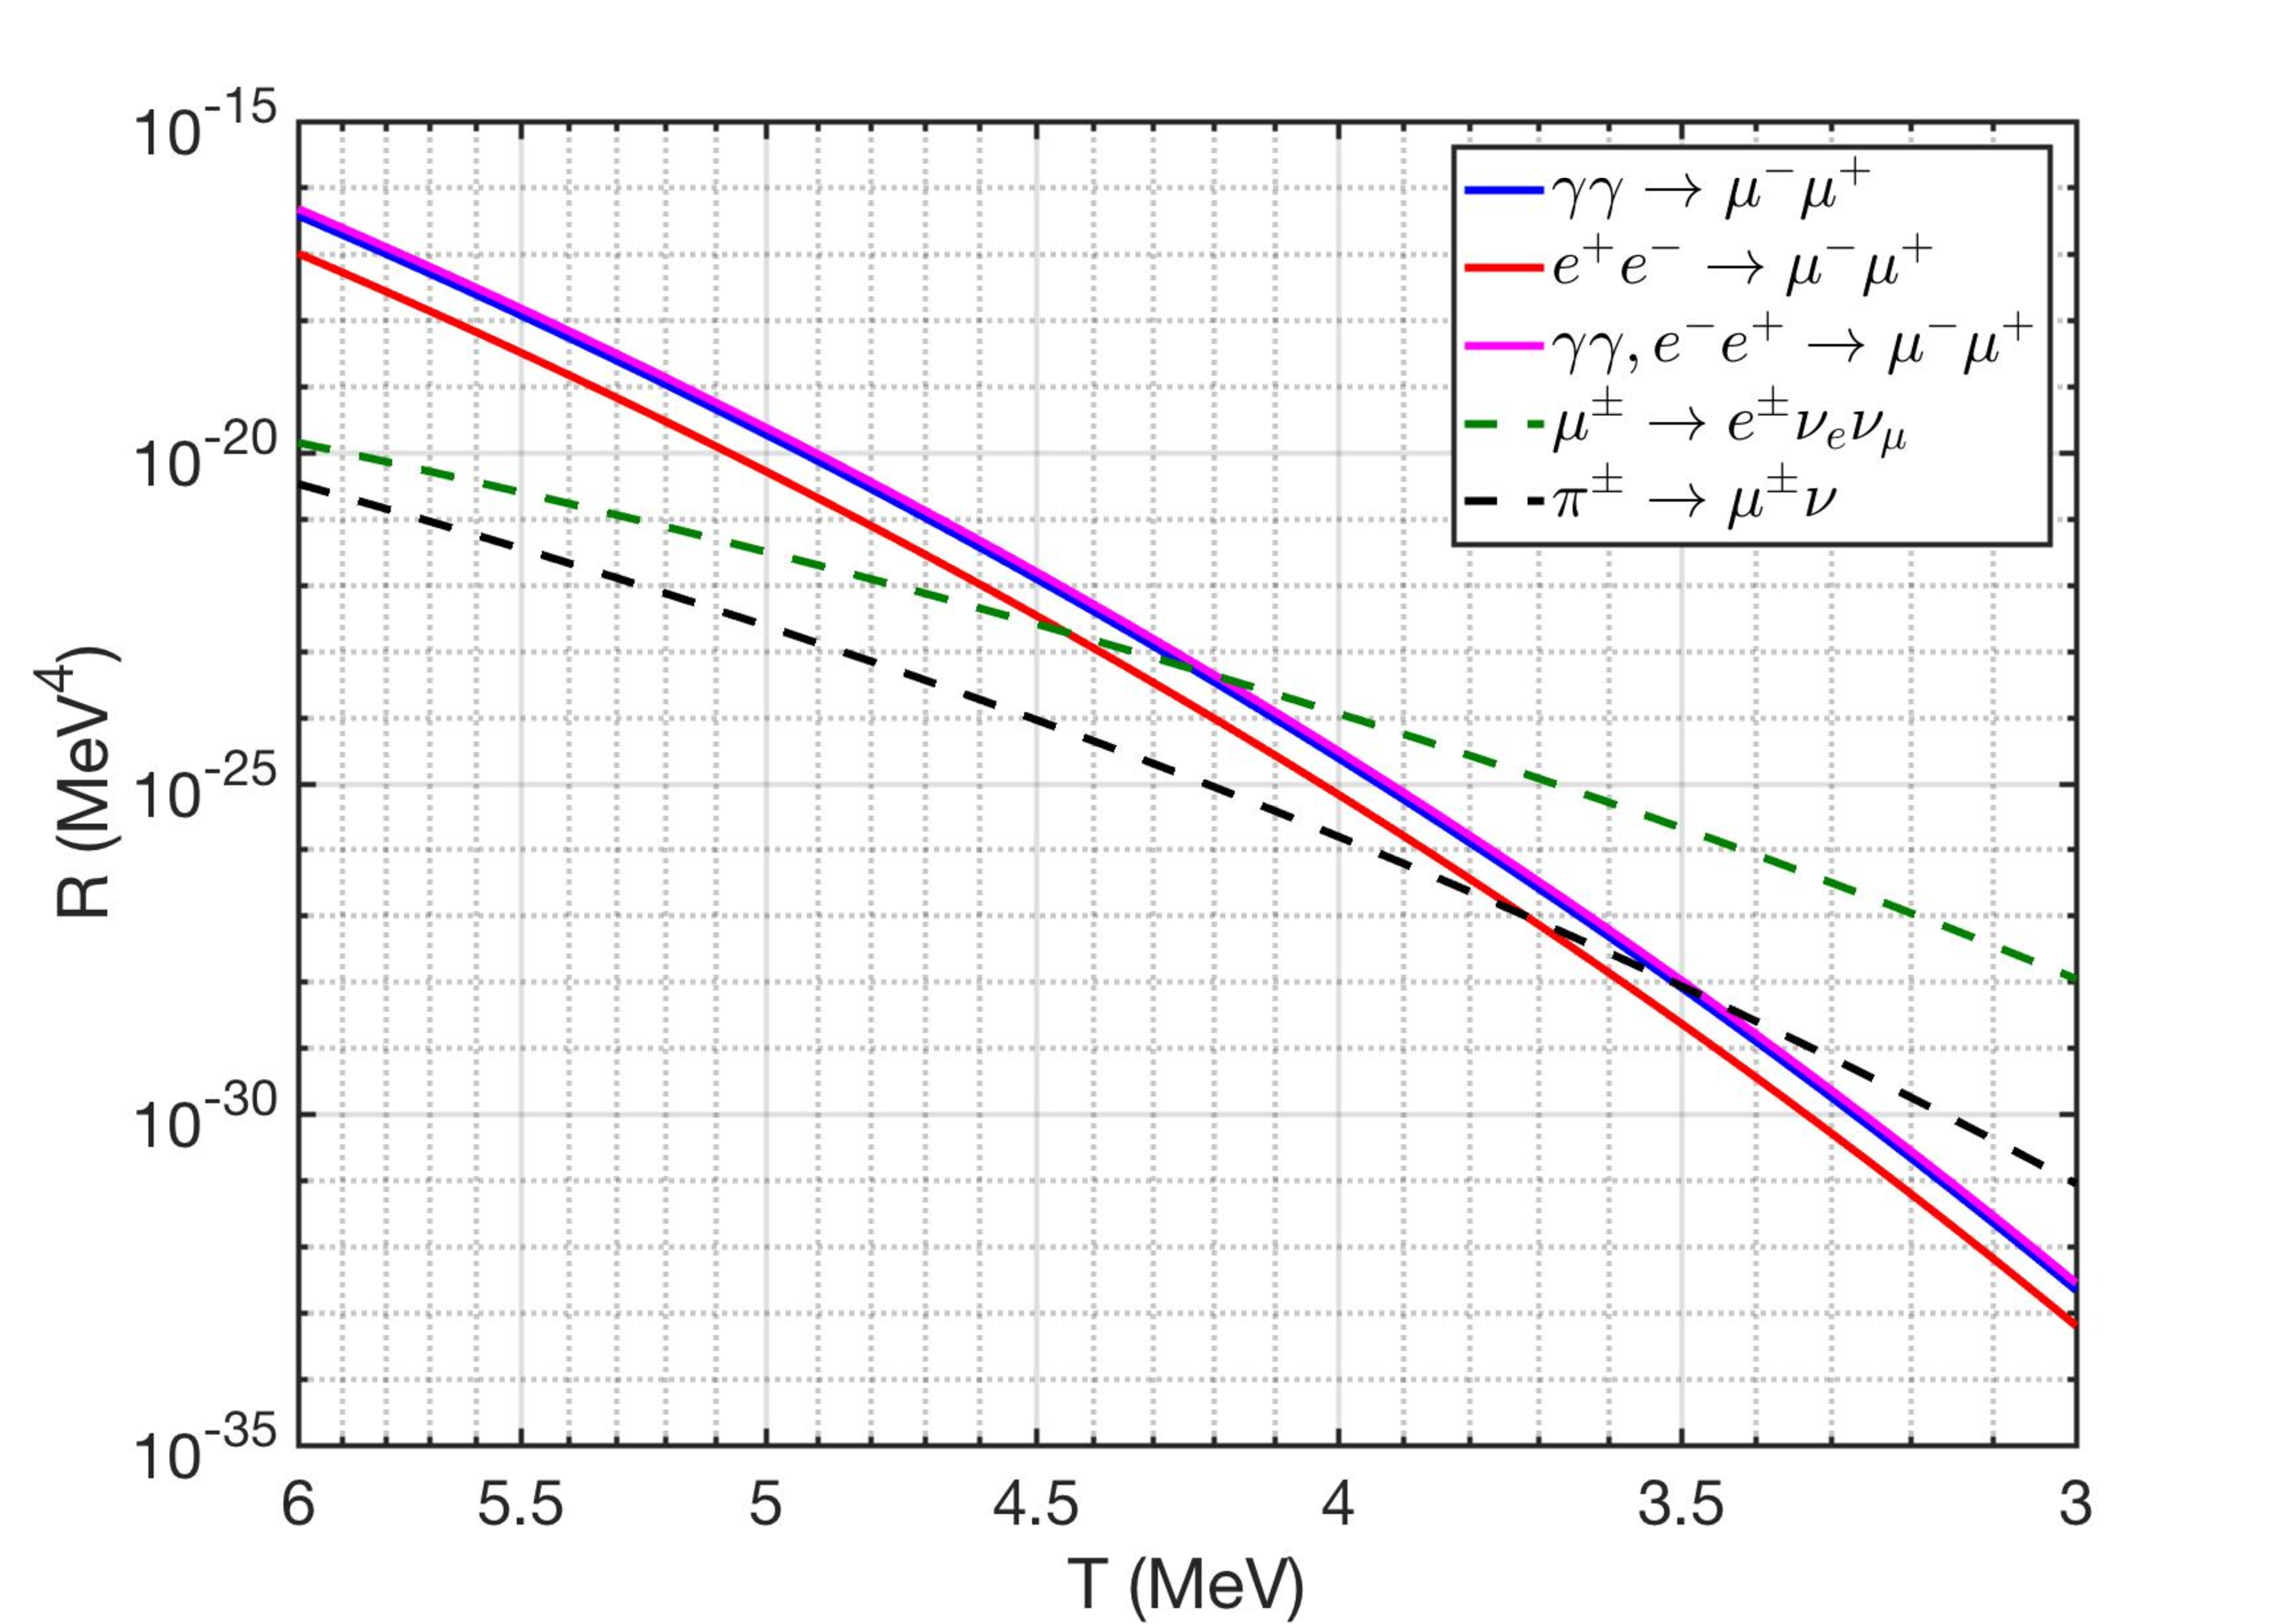
\includegraphics[width=5.0in]{./plots/MuonRate_new2.pdf}
\caption{We plot the thermal reaction rate per volume for different reactions as a function of temperature. We found that dominant reactions for $\mu^\pm$ production are ${\gamma+\gamma\to\mu^++\mu^-}$ and $e^++e^-\to\mu^++\mu^-$, and the total production rate crosses the decay rate of $\mu^\pm$ at temperature $T_{dissapear}\approx 4.195$ MeV.}
\label{MuonRatenew_fig}
\end{center}
\end{figure}
%~~~~~~~~~~~~~~~~~~~~~~~~~~~~~~~~~~~~~~~~~~~~~~~~~~~~~~~~~~~~~~~~~~~~~~~~~~~~~~~~~~~~~~~~~~~~~~~~

On the other hand, considering the number density for nonrelativistic $\mu^\pm$ in the Boltzmann approximation, we have
\begin{align}\label{nmupm}
n_{\mu^\pm}=\frac{g_{\mu^\pm}}{2\pi^2}T^3\left(\frac{m_\mu}{T}\right)^2 K_2(m_\mu/T)=g_{\mu^\pm}\left(\frac{m_\mu T}{2\pi}\right)^{3/2}e^{-{m_\mu}/{T}}\;. 
\end{align}
then the number density between $n_{\mu^\pm}$ and baryon $n_B$ can be written as
\begin{align}
\frac{n_{\mu^\pm}}{n_\mathrm{B}}=\frac{n_{\mu^\pm}}{s}\frac{s}{n_\mathrm{B}}=
\frac{n_{\mu^\pm}}{s}\left(\frac{s}{n_\mathrm{B}}\right)_{\!t_0},
\end{align}
where we used that $s/n_\mathrm{B}$ remains constant and $t_0$ represent present day value. The present value is given by $(n_B/s)_{t_0}\approx8.69\times10^{-11}$ (detail please see Chapter~\ref{Introduction}). The entropy density $s$ can be characterized introducing $g^s_\ast$, the total number of \lq entropic\rq\ degrees of freedom
\begin{align}\label{entrop}
s=\frac{2\pi^2}{45}g^s_\ast T^3\;.
\end{align}
For temperature $10\,\mathrm{MeV} >T>3 $\,MeV, the massless photons, nearly relativistic electron/positrons, and practically massless neutrinos contribute to the degree of freedom $g^s_\ast$.  In this case, the number density between $n_{\mu^\pm}$ and baryon $n_B$ in the temperature interval we consider $10\,\mathrm{MeV} >T>3 $\,MeV is given by
\begin{align}\label{nmuperbF} 
\frac{n_{\mu^\pm}}{n_\mathrm{B}}=\frac{45}{2\pi^2}\frac{g_{\mu^\pm}}{g^s_\ast}\left(\frac{m_\mu}{2\pi T}\right)^{3/2}e^{-{m_\mu}/{T}}\;\left(\frac{s}{n_\mathrm{B}}\right)_{\!t_0}.
\end{align}


%Figure~~~~~~~~~~~~~~~~~~~~~~~~~~~~~~~~~~~~~~~~~~~~~~~~~~~~~~~~~~~~~~~~~~~~~~~~~
\begin{figure}[t]
\begin{center}
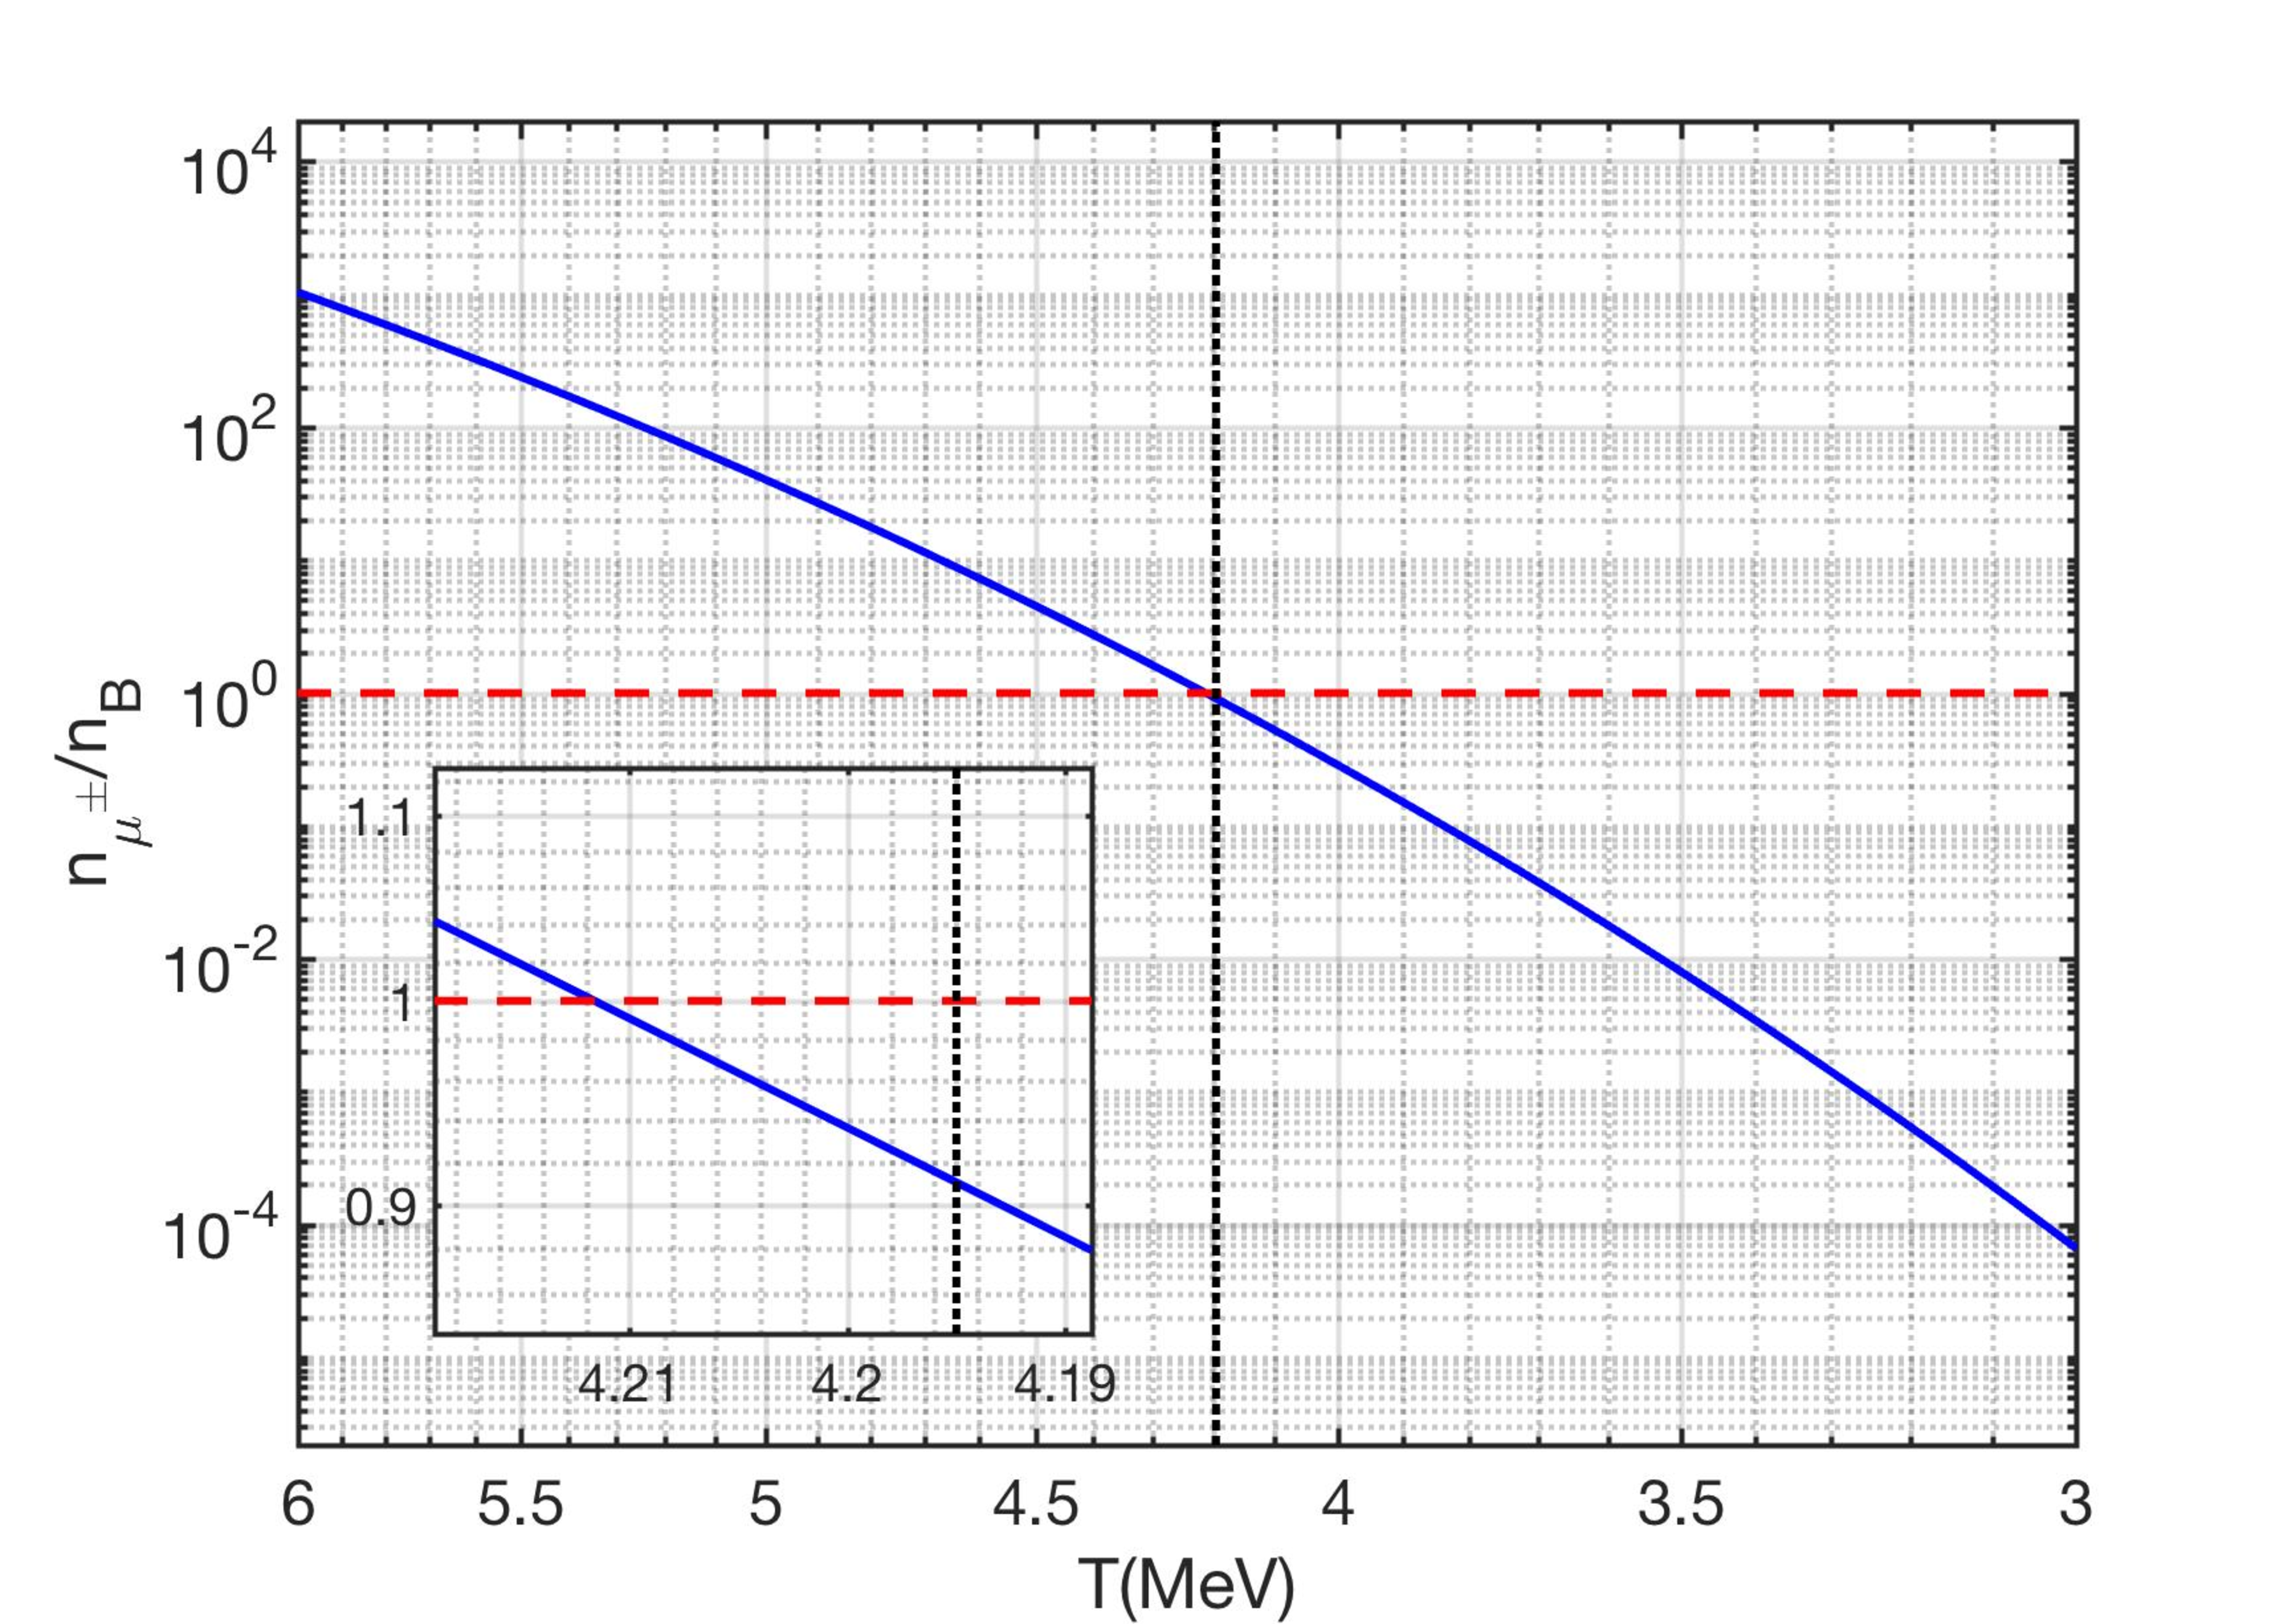
\includegraphics[width=\linewidth]{./plots/DensityRatio_new2.pdf}
\caption{
The density ratio between $\mu^\pm$ and baryons as a function of temperature. The density ratio at muon disappearance temperature is about $n_{\mu^\pm}/n_\mathrm{B}(T_\mathrm{disappear})\approx0.911$, and around the temperature $T\approx4.212$ MeV the density ratio $n_{\mu^\pm}/n_\mathrm{B}\approx1$.}
\label{DensityRatio_fig}
\end{center}
\end{figure}
%~~~~~~~~~~~~~~~~~~~~~~~~~~~~~~~~~~~~~~~~~~~~~~~~~~~~~~~~~~~~~~~~~~~~~~~~~~~~~


In Fig.\,\ref{DensityRatio_fig} we show the muon to baryon density ratio Eq.\,(\ref{nmuperbF}) as a function of $T$. We see that the muon abundance $T=10$\,MeV exceeds that of baryons by a factor 500,000 while at muon disappearance temperature $n_{\mu^\pm}/n_\mathrm{B}(T_\mathrm{disappear})\approx0.911$. The number density $n_{\mu^\pm}$ and $n_\mathrm{B}$  abundances are equal at around the temperature $T_\mathrm{equal}\approx4.212\,\mathrm{MeV} >  T_\mathrm{disappear}$.  This means that the muon abundance may still be able to influence baryon evolution because their number density is comparable to the baryon density.% However, we also find that at the temperature $T_\mathrm{equal}\approx4.212$\,MeV the density ratio is unity $n_{\mu^\pm}/n_\mathrm{B}\approx1$.

The primary insight of this work is that aside of protons, neutrons and other nonrelativistic particles, both positively and negatively charged muons $\mu^\pm$ are present in thermal equilibrium and in non-negligible abundance for $T>T_\mathrm{dissapear}\approx 4.195$\,MeV. This offers a new and tantalizing model building opportunity for anyone interested in baryon-antibaryon separation in the primordial Universe, strangelet formation, and perhaps other exotic primordial structure formation mechanisms.

%%%%%%%%%%%%%%%%%%%%%%%%
\include{03-birrell/birrell}
%%%%%%%%%%%%%%%%%%%%%%%%
\include{04-grayson/grayson}
%%%%%%%%%%%%%%%%%%%%%%%%
%%%%%%%%%%%%%%%%%%%%%%%%%%%%%%%%%%%%%%%
%\chapter{Matter-antimatter origin of cosmic magnetism}
%\label{chap:cosmo}
%%%%%%%%%%%%%%%%%%%%%%%%%%%%%%%%%%%%%%%
\noindent We investigate the hypothesis that the observed intergalactic magnetic fields (IGMF) are primordial in nature, predating the recombination epoch. Specifically, we explore the role of the extremely large electron-positron $(e^{+}e^{-})$ pair abundance in the temperature range of $2000\keV>T>20\keV$ which only disappeared after Big Bang nucleosynthesis (BBN). We review the status of cosmic magnetism in \rsec{sec:universe} which motivates our study. \rsec{sec:abundance} discusses the extreme electron-positron abundance during this epoch. The statistical and thermodynamic theory of the electron-positron gas is described in \rsec{sec:theory}. \rsec{sec:magnetization} describes the relativistic paramagnetism of the electron-positron gas. We propose in \rsec{sec:ferro} a model of self-magnetization caused by spin polarization within the individual species in the gas.

This chapter serves primarily as a review of our work in~\cite{Steinmetz:2023nsc,Steinmetz:2023ucp} and portions of~\cite{Rafelski:2023emw} where we propose that the early universe electron-positron plasma was a highly magnetized environment. We will use natural units $(c=\hbar=k_{B}=1)$ unless otherwise noted.

%%%%%%%%%%%%%%%%%%%%%%%%%%%%%%%%%%%%%%%
\section{Short survey of magnetism in the universe}
\label{sec:universe}
%%%%%%%%%%%%%%%%%%%%%%%%%%%%%%%%%%%%%%%
\noindent Macroscopic domains of magnetic fields have been found in all astrophysical environments from compact objects (stars, planets, etc.); interstellar and intergalactic space; and surprisingly in deep extra-galactic void spaces. Considering the ubiquity of magnetic fields in the universe~\cite{Giovannini:2017rbc,Giovannini:2003yn,Kronberg:1993vk}, we search for a common primordial mechanism initiate the diversity of magnetism observed today. In this chapter, IGMF will refer to experimentally observed intergalactic fields of any origin while primordial magnetic fields (PMF) refers to fields generated via early universe processes possibly as far back as inflation. The conventional elaboration of the origins for cosmic PMFs are detailed in~\cite{Gaensler:2004gk,Durrer:2013pga,AlvesBatista:2021sln}.

IGMF are notably difficult to measure and difficult to explain. The bounds for IGMF at a length scale of $1{\rm\ Mpc}$ are today~\cite{Neronov:2010gir,Taylor:2011bn,Pshirkov:2015tua,Jedamzik:2018itu,Vernstrom:2021hru}
\begin{gather}
 \label{igmf}
 10^{-8}{\rm\ G}>B_\mathrm{IGMF}>10^{-16}{\rm\ G}\,.
\end{gather}
We note that generating PMFs with such large coherent length scales is nontrivial~\cite{Giovannini:2022rrl} though currently the length scale for PMFs are not well constrained~\cite{AlvesBatista:2021sln}. Faraday rotation from distant radio active galaxy nuclei (AGN)~\cite{Pomakov:2022cem} suggest that neither dynamo nor astrophysical processes would sufficiently account for the presence of magnetic fields in the universe today if the IGMF strength was around the upper bound of $B_\mathrm{IGMF}\simeq30-60{\rm\ nG}$ as found in Ref.~\cite{Vernstrom:2021hru}. Such strong magnetic fields would then require that at least some portion of the IGMF arise from primordial sources that predate the formation of stars.

Magnetized baryon inhomogeneities which in turn would produce anisotropies in the cosmic microwave background (CMB)~\cite{Jedamzik:2013gua,Abdalla:2022yfr}. \cite{Jedamzik:2020krr} propose further that the presence of a magnetic field of $B_\mathrm{PMF}\simeq0.1{\rm\ nG}$ could be sufficient to explain the Hubble tension.

%%%%%%%%%%%%%%%%%%%%%%%%%%%%%%%%%%%%%%%
\begin{figure}[ht]
    \centering
    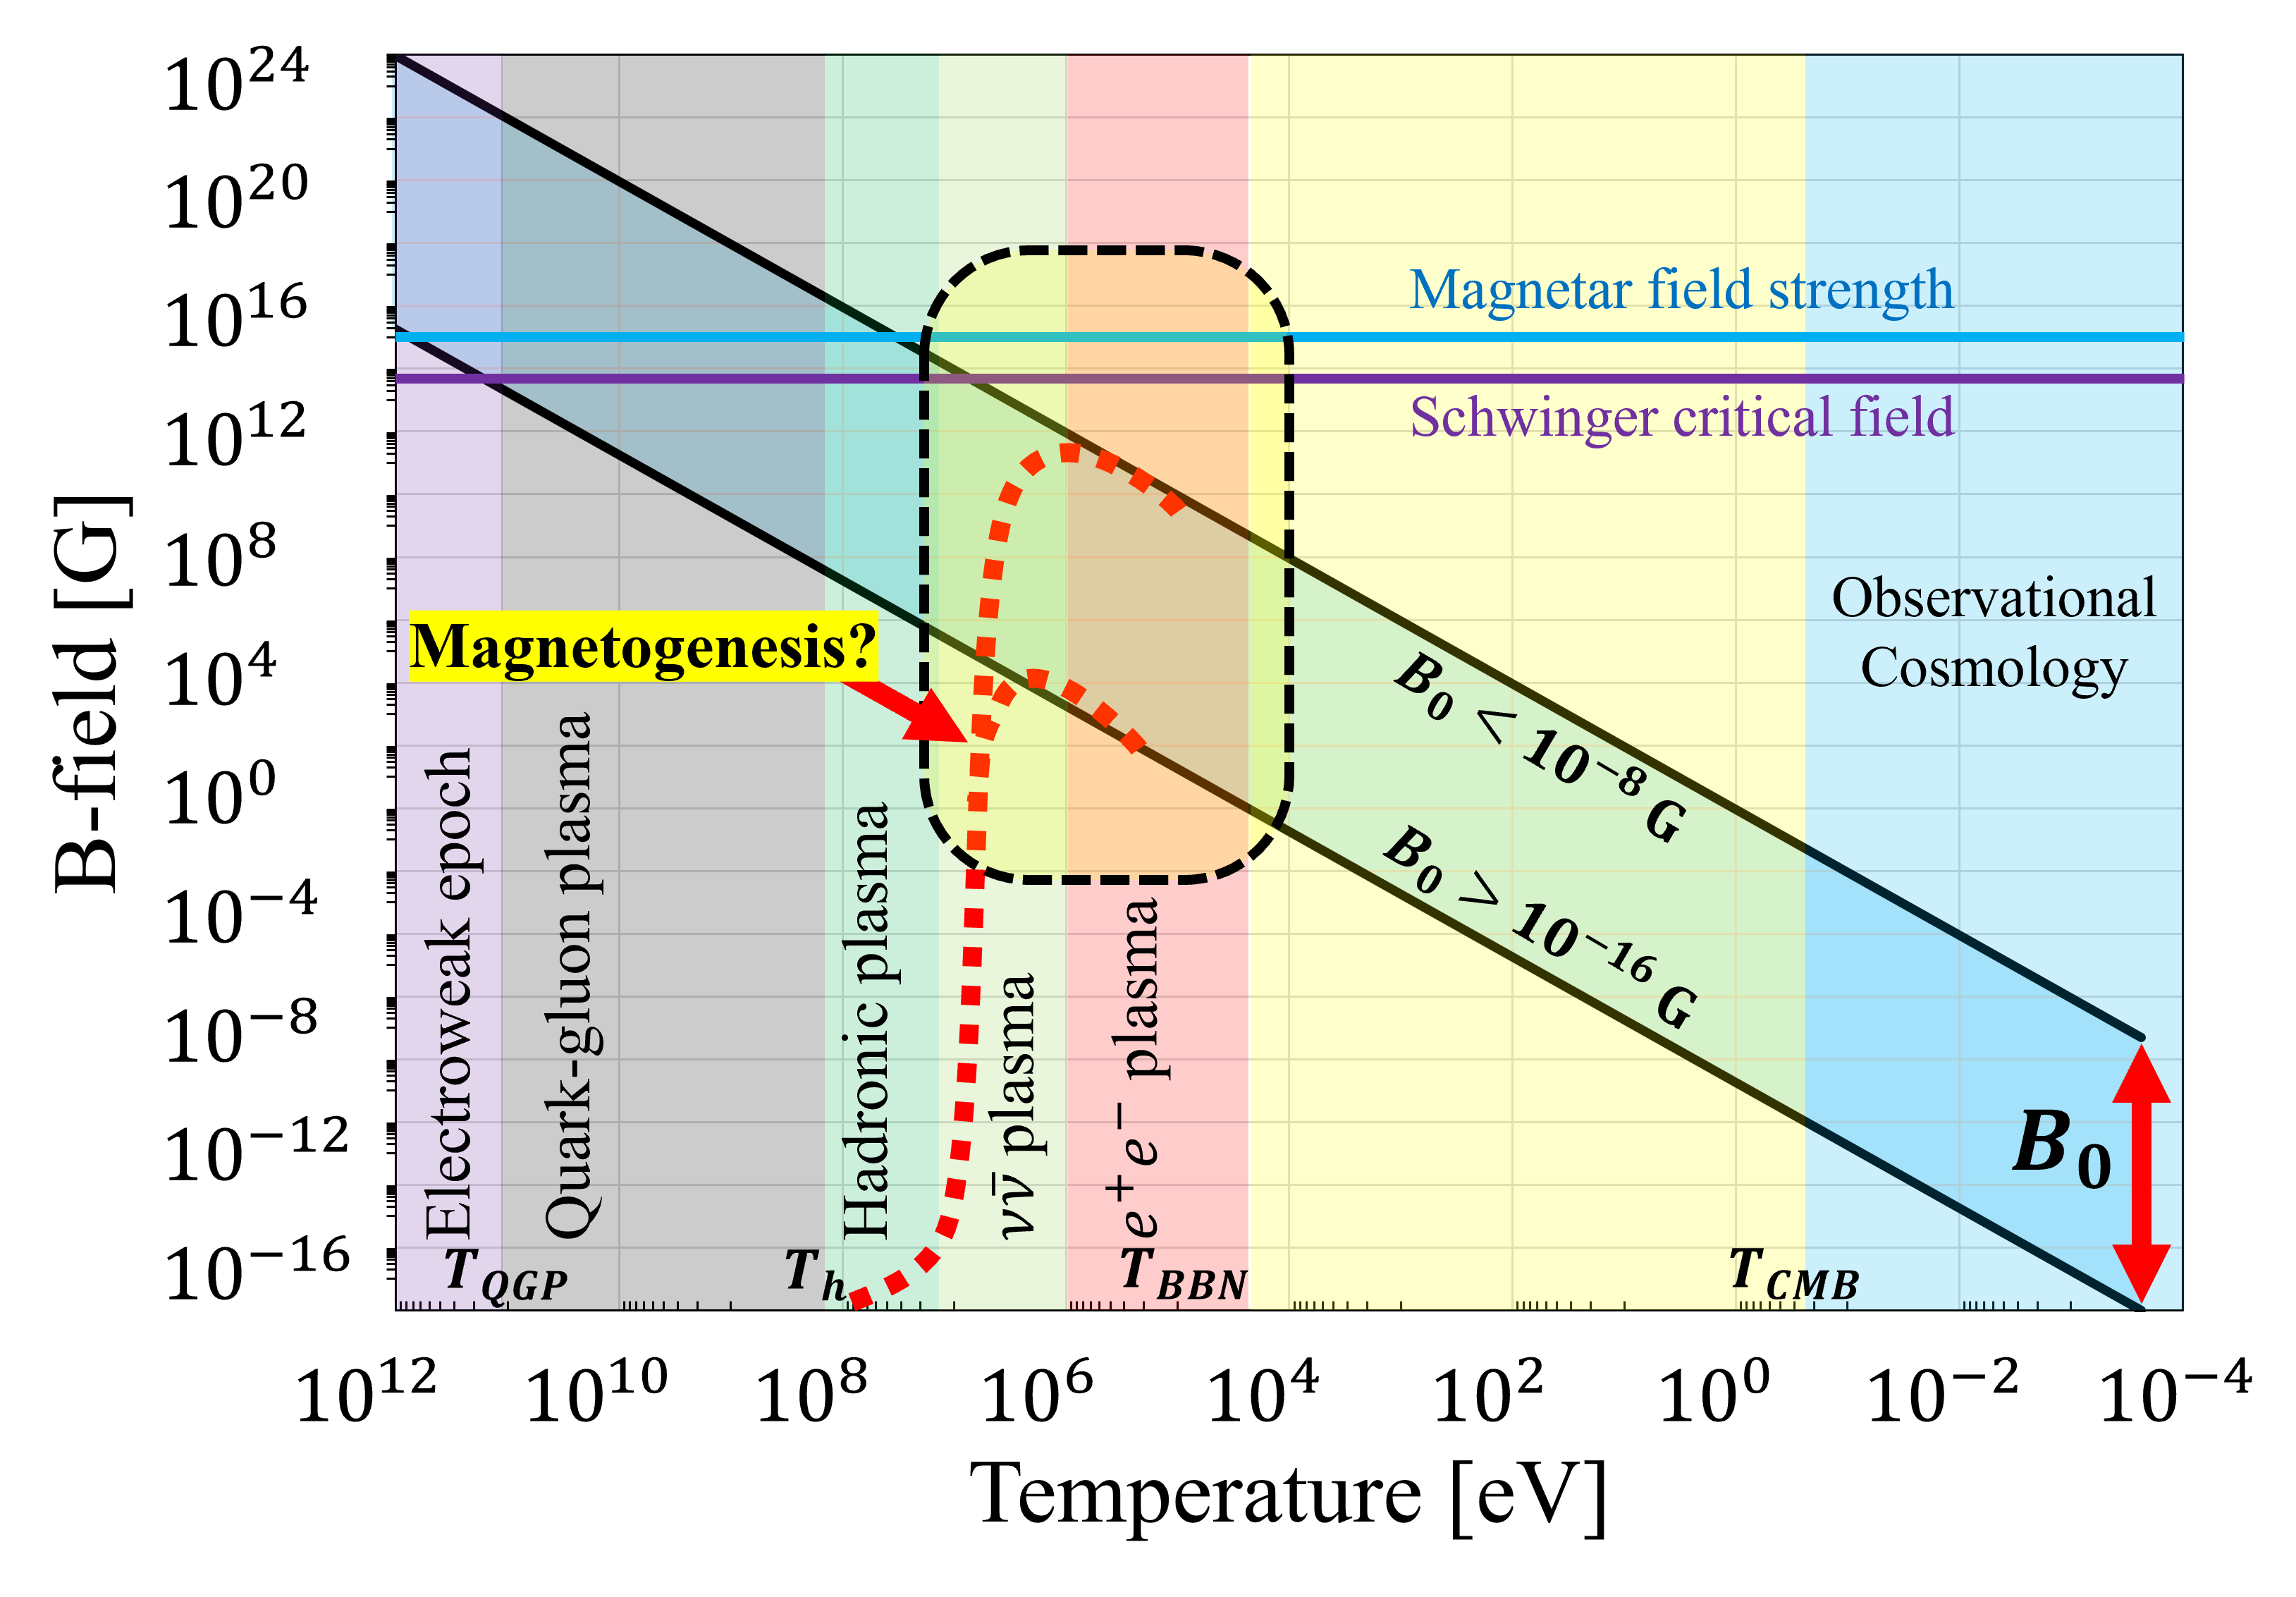
\includegraphics[width=0.95\textwidth]{plots/chap04cosmo/pmf.png}
    \caption{Qualitative plot of the primordial magnetic field strength over cosmic time. All figures are printed in temporal sequence in the expanding universe beginning with high temperatures (and early times) on the left and lower temperatures (and later times) on the right.}
    \label{fig:pmf}
\end{figure}
%%%%%%%%%%%%%%%%%%%%%%%%%%%%%%%%%%%%%%%

Our motivating hypothesis is outlined qualitatively in \rf{fig:pmf} where PMF evolution is plotted over the temperature history of the universe. The descending blue band indicates the range of possible PMF strengths. The different epochs of the universe according to $\Lambda\mathrm{CDM}$ are delineated by temperature. The horizontal lines mark two important scales: (a) the Schwinger critical field strength given by
\begin{align}
    \label{crit:1}
    B_\mathrm{C} = \frac{m_{e}^{2}}{e}\simeq4.41\times10^{13}\,\mathrm{G}\,.
\end{align}
where electrodynamics is expected to display nonlinear characteristics and (b) the upper field strength seen in magnetars of $\sim10^{15}\,\mathrm{G}$. A schematic of magnetogenesis is drawn with the dashed red lines indicating spontaneous formation of the PMF within the early universe plasma itself. The $e^{+}e^{-}$ era is notably the final epoch where antimatter exists in large quantities in the cosmos~\cite{Rafelski:2023emw}.

%%%%%%%%%%%%%%%%%%%%%%%%%%%%%%%%%%%%%%%
\section{Electron-positron abundance}
\label{sec:abundance}
%%%%%%%%%%%%%%%%%%%%%%%%%%%%%%%%%%%%%%%
\noindent As the universe cooled below temperature $T\!=\!m_{e}$ (the electron mass), the thermal electron and positron comoving density depleted by over eight orders of magnitude. At $T_\mathrm{split}=20.3\keV$, the charged lepton asymmetry (mirrored by baryon asymmetry and enforced by charge neutrality) became evident as the surviving excess electrons persisted while positrons vanished entirely from the particle inventory of the universe due to annihilation.

%%%%%%%%%%%%%%%%%%%%%%%%%%%%%%%%%%%%%%%
\begin{figure}[ht]
 \centering
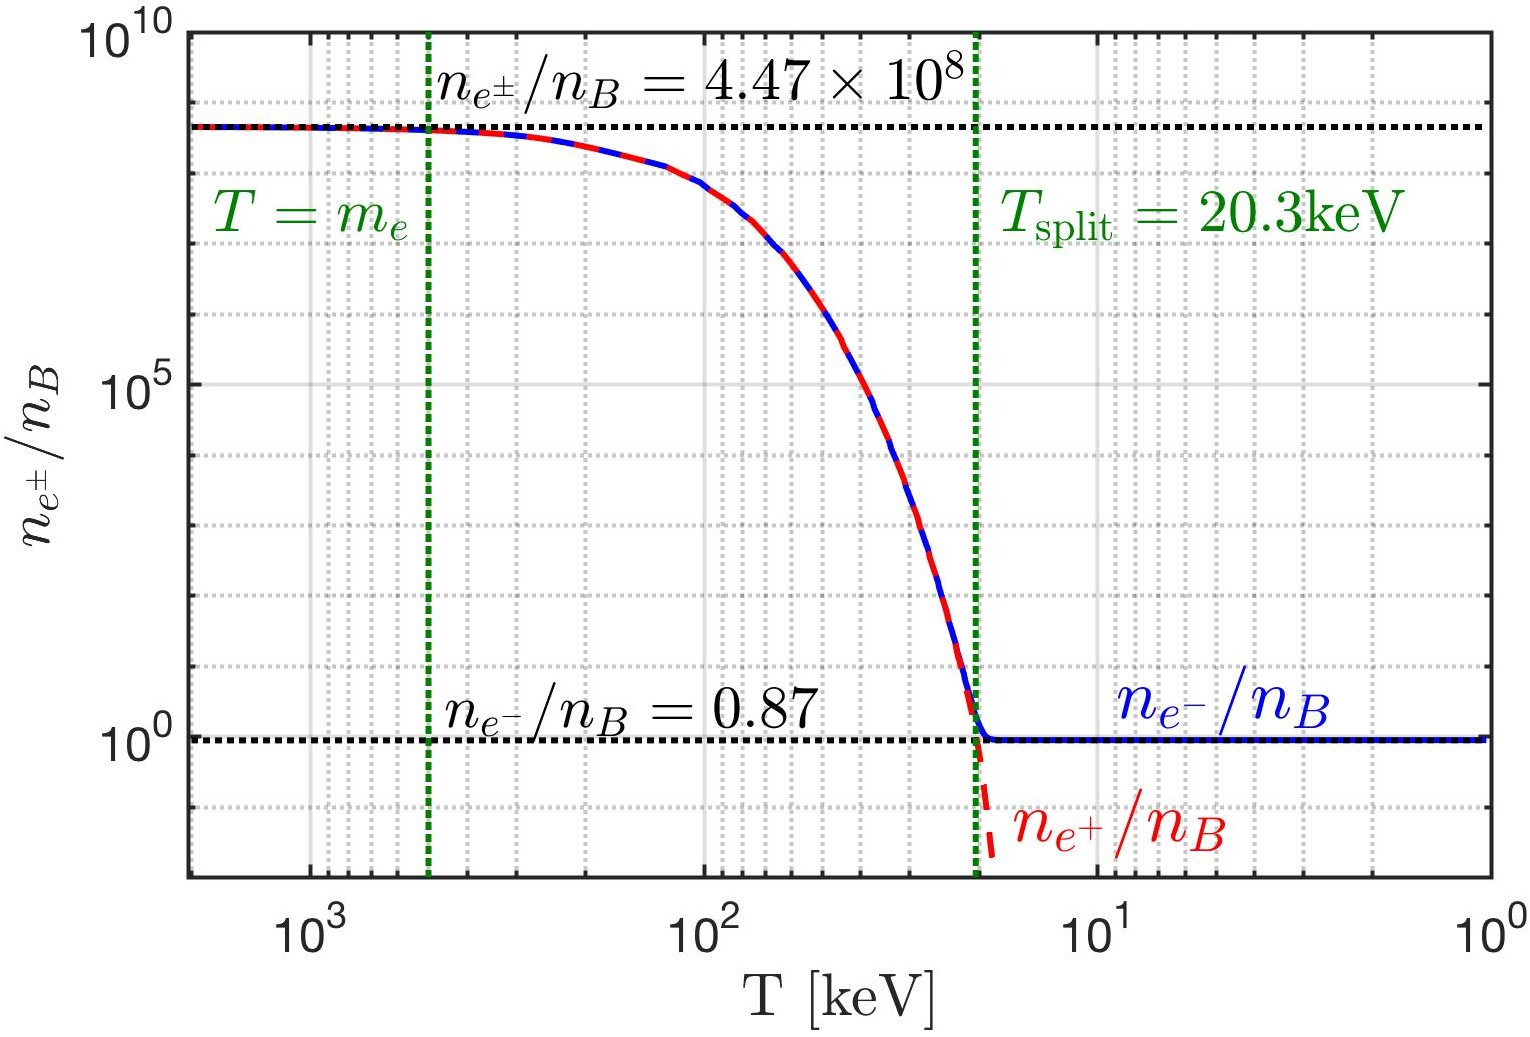
\includegraphics[width=0.95\textwidth]{plots/chap04cosmo/EEPlasmaDensityRatio_new01.jpg}
 \caption{Number density of electron $e^{-}$ and positron $e^{+}$ to baryon ratio $n_{e^{\pm}}/n_{B}$ as a function of photon temperature in the universe. See text for further details. In this work we measure temperature in units of energy (keV) thus we set the Boltzmann constant to $k_{B}=1$. Figure courtesy of Cheng Tao Yang.}
 \label{fig:densityratio} 
\end{figure}
%%%%%%%%%%%%%%%%%%%%%%%%%%%%%%%%%%%%%%%

The electron-to-baryon density ratio $n_{e^{-}}/n_{B}$ is shown in \rf{fig:densityratio} as the solid blue line while the positron-to-baryon ratio $n_{e^{+}}/n_{B}$ is represented by the dashed red line. These two lines overlap until the temperature drops below $T_\mathrm{split}=20.3\keV$ as positrons vanish from the universe marking the end of the $e^{+}e^{-}$ plasma and the dominance of the electron-proton $(e^{-}p)$ plasma. The two vertical dashed green lines denote temperatures $T\!=\!m_{e}\simeq511\keV$ and $T_\mathrm{split}=20.3\keV$. These results were obtained using charge neutrality and the baryon-to-photon content (entropy) of the universe; see details in~\cite{Rafelski:2023emw}. The two horizontal black dashed lines denote the relativistic $T\gg m_e$ abundance of $n_{e^{\pm}}/n_{B}=4.47\times10^{8}$ and post-annihilation abundance of $n_{e^{-}}/n_{B}=0.87$. Above temperature $T\simeq85\keV$, the $e^{+}e^{-}$ primordial plasma density exceeded that of the Sun's core density $n_{e}\simeq6\times10^{26}{\rm\ cm}^{-3}$~\cite{Bahcall:2000nu}. 

Conversion of the dense $e^{+}e^{-}$ pair plasma into photons reheated the photon background~\cite{Birrell:2014uka} separating the photon and neutrino temperatures. The $e^{+}e^{-}$ annihilation and photon reheating period lasted no longer than an afternoon lunch break. Because of charge neutrality, the post-annihilation comoving ratio $n_{e^{-}}/n_{B}=0.87$~\cite{Rafelski:2023emw} is slightly offset from unity in~\rf{fig:densityratio} by the presence of bound neutrons in $\alpha$ particles and other neutron containing light elements produced during BBN epoch.

The abundance of baryons is itself fixed by the known abundance relative to photons~\cite{ParticleDataGroup:2022pth} and we employed the contemporary recommended value $n_B/n_\gamma=6.09\times 10^{-10}$. The resulting chemical potential needs to be evaluated carefully to obtain the behavior near to $T_\mathrm{split}=20.3\keV$ where the relatively small value of chemical potential $\mu$ rises rapidly so that positrons vanish from the particle inventory of the universe while nearly one electron per baryon remains. The detailed solution of this problem is found in \cite{Fromerth:2012fe,Rafelski:2023emw} leading to the results shown in \rf{fig:densityratio}.

%%%%%%%%%%%%%%%%%%%%%%%%%%%%%%%%%%%%%%%
\section{Theory of thermal matter-antimatter plasmas}
\label{sec:theory}
%%%%%%%%%%%%%%%%%%%%%%%%%%%%%%%%%%%%%%%
\noindent To evaluate magnetic properties of the thermal $e^{+}e^{-}$ pair plasma we take inspiration from Ch. 9 of Melrose's treatise on magnetized plasmas~\cite{melrose2008quantum}. We focus on the bulk properties of thermalized plasmas in (near) equilibrium.

We consider a homogeneous magnetic field domain defined along the $z$-axis as
\begin{gather}
    \label{homoB:1}
    \bb{B}=(0,\,0,\,B)\,,
\end{gather}
with magnetic field magnitude $|\bb{B}|=B$. Following \rchap{chap:moment}, we reprint the microscopic energy (\req{lan24b} in different notation) of the charged relativistic fermion within a homogeneous magnetic field given by
\begin{align}
 \label{cosmokgp}
 E^{n}_{\sigma,s}(p_{z},{B})=\sqrt{m_{e}^{2}+p_{z}^{2}+e{B}\left(2n+1+\frac{g}{2}\sigma s\right)}\,,
\end{align}
where $n\in0,1,2,\ldots$ is the Landau orbital quantum number, $p_{z}$ is the momentum parallel to the field axis and the electric charge is $e\equiv q_{e^{+}}=-q_{e^{-}}$. The index $\sigma$ in \req{cosmokgp} differentiates electron $(e^{-};\ \sigma=+1)$ and positron $(e^{+};\ \sigma=-1)$ states. The index $s$ refers to the spin along the field axis: parallel $(\uparrow;\ s=+1)$ or anti-parallel $(\downarrow;\ s=-1)$ for both particle and antiparticle species.

%%%%%%%%%%%%%%%%%%%%%%%%%%%%%%%%%%%%%%%
\begin{figure}[ht]
 \centering
 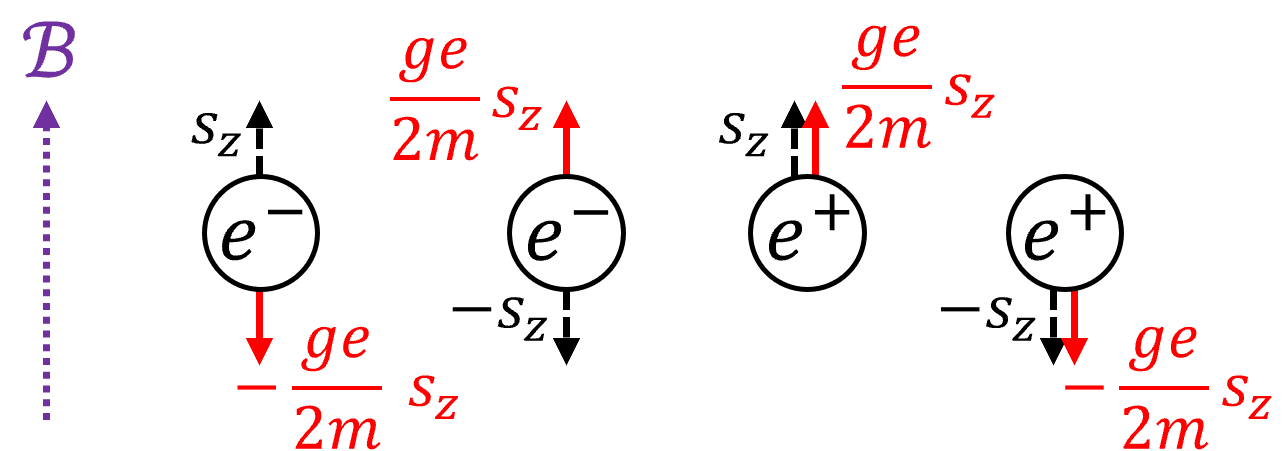
\includegraphics[width=0.95\linewidth]{plots/chap04cosmo/schematic.png}\Bstrut\\
 \begin{tabular}{ r|c|c| }
 \multicolumn{1}{r}{}
 & \multicolumn{1}{c}{aligned: $s=+1$}
 & \multicolumn{1}{c}{anti-aligned: $s=-1$} \\
 \cline{2-3}
 electron: $\sigma=+1$ & $U_{\rm Mag}>0$ & $U_{\rm Mag}<0$ \TBstrut\\
 \cline{2-3}
 positron: $\sigma=-1$ & $U_{\rm Mag}<0$ & $U_{\rm Mag}>0$ \TBstrut\\
 \cline{2-3}
 \end{tabular}\\
 \caption{Organizational schematic of matter-antimatter $(\sigma)$ and polarization $(s)$ states with respect to the sign of the non-relativistic magnetic dipole energy $U_{\rm Mag}$ obtainable from~\req{cosmokgp}.}
 \label{fig:schematic}
\end{figure}
%%%%%%%%%%%%%%%%%%%%%%%%%%%%%%%%%%%%%%%

The reason \req{cosmokgp} distinguishes between electrons and positrons is to ensure the correct non-relativistic limit for the magnetic dipole energy is reached. Following the conventions found in \cite{Tiesinga:2021myr}, we set the gyro-magnetic factor $g\equiv g_{e^{+}}=-g_{e^{-}}>0$ such that electrons and positrons have opposite $g$-factors and opposite magnetic moments relative to their spin; see \rf{fig:schematic}.

We recall the conventions established in \rsec{sec:flrw}. Conservation of magnetic flux requires that the magnetic field through a comoving surface $L_{0}^{2}$ remain unchanged. The magnetic field strength under expansion~\cite{Durrer:2013pga} starting at some initial time $t_{0}$ is then given by
\begin{gather}
 \label{bscale}
 B(t)=B_{0}\frac{a^{2}_{0}}{a^{2}(t)}\rightarrow B(z)=B_{0}\left(1+z\right)^{2}\,,
\end{gather}
where $B_{0}$ is the comoving value obtained from the contemporary value of the magnetic field today. Magnetic fields in the cosmos generated through mechanisms such as dynamo or astrophysical sources do not follow this scaling~\cite{Pomakov:2022cem}. It is only in deep intergalactic space where matter density is low are magnetic fields preserved (and thus uncontaminated) over cosmic time.

From \req{tscale} and \req{bscale} there emerges a natural ratio of interest which is conserved over cosmic expansion 
\begin{gather}
 \label{tbscale}
 \boxed{b\equiv\frac{e{B}(t)}{T^{2}(t)}=\frac{e{B}_{0}}{T_{0}^{2}}\equiv b_0={\rm\ const.}}\\
 10^{-3}>b_{0}>10^{-11}\,,
\end{gather}
given in natural units ($c=\hbar=k_{B}=1$). We computed the bounds for this cosmic magnetic scale ratio by using the present day IGMF observations given by \req{igmf} and the present CMB temperature $T_{0}=2.7{\rm\ K}\simeq2.3\times10^{-4}\eV$~\cite{Planck:2018vyg}.

%%%%%%%%%%%%%%%%%%%%%%%%%%%%%%%%%%%%%%%
\subsection{Eigenstatess of magnetic moment in cosmology}
\label{sec:protection}
%%%%%%%%%%%%%%%%%%%%%%%%%%%%%%%%%%%%%%%

As statistical properties depend on the characteristic Boltzmann factor $E/T$, another interpretation of \req{tbscale} in the context of energy eigenvalues (such as those given in \req{cosmokgp}) is the preservation of magnetic moment energy relative to momentum under adiabatic cosmic expansion. The Boltzmann statistical factor is given by
\begin{alignat}{1}
    \label{Boltz} x\equiv\frac{E}{T}\,.
\end{alignat}
We can explore this relationship for the magnetized system explicitly by writing out \req{Boltz} using the KGP energy eigenvalues written in \req{cosmokgp} as
\begin{alignat}{1}
    \label{XExplicit} x_{\sigma,s}^{n} = \frac{E_{\sigma,s}^{n}}{T} = \sqrt{\frac{m_{e}^{2}}{T^{2}}+\frac{p_{z}^{2}}{T^{2}}+\frac{eB}{T^{2}}\left(2n+1+\frac{g}{2}\sigma s\right)}\,.
\end{alignat}

Introducing the expansion scale factor $a(t)$ via \req{tscale}, \req{bscale} and \req{tbscale}. The Boltzmann factor can then be written as
\begin{alignat}{1}
    \label{xscale:1} x_{\sigma,s}^{n}(a(t)) = \sqrt{\frac{m_{e}^{2}}{T^{2}(t_{0})}\frac{a(t)^{2}}{a_{0}^{2}}+\frac{p_{z,0}^{2}}{T_{0}^{2}}+\frac{eB_{0}}{T_{0}^{2}}\left(2n+1+\frac{g}{2}\sigma s\right)}\,.
\end{alignat}
This reveals that only the mass contribution is dynamic over cosmological time. The constant of motion $b_{0}$ defined in \req{tbscale} is seen as the coefficient to the Landau and spin portion of the energy. For any given eigenstate, the mass term drives the state into the non-relativistic limit while the momenta and magnetic contributions are frozen by initial conditions. 

In comparison, the Boltzmann factor for the DP energy eigenvalues are given by
\begin{alignat}{1}
    \label{xscaledp:1} x_{\sigma,s}^{n}\vert_\mathrm{DP} = \sqrt{\left(\sqrt{\frac{m_{e}^{2}}{T^{2}}+\frac{eB}{T^{2}}\left(2n+1+\sigma s\right)}+\frac{eB}{2m_{e}T}\left(\frac{g}{2}-1\right)\sigma s\right)^{2}+\frac{p_{z}^{2}}{T^{2}}}\,,
\end{alignat}
which scales during FLRW expansion as
\begin{multline}
    \label{xscaledp:2} x_{\sigma,s}^{n}(a(t))\vert_\mathrm{DP} =\\ \sqrt{\left(\sqrt{\frac{m_{e}^{2}}{T_{0}^{2}}\frac{a(t)^{2}}{a_{0}^{2}}+\frac{eB_{0}}{T_{0}^{2}}\left(2n+1+\sigma s\right)}+\frac{eB_{0}}{2m_{e}T_{0}}\frac{a_{0}}{a(t)}\left(\frac{g}{2}-1\right)\sigma s\right)^{2}+\frac{p_{z,0}^{2}}{T_{0}^{2}}}\,.
\end{multline}
While the above expression is rather complicated, we note that the KGP~\req{xscale:1} and DP~\req{xscaledp:1} Boltzmann factors both reduce to the Sch{\"o}dinger-Pauli limit as $a(t)\rightarrow\infty$ thereby demonstrating that the total magnetic moment is protected under the adiabatic expansion of the universe.

As noted in in \rsec{sec:ikgp} and \rsec{sec:emmass}, higher order non-minimal magnetic contributions can be introduced to the Boltzmann factor such as $\sim(e/m)^{2}B^{2}/T^{2}$. The reasoning above suggests that these terms are suppressed over cosmological time driving the system into minimal electromagnetic coupling with the exception of the anomalous magnetic moment. It is interesting to note that cosmological expansion then serves to `smooth out' the characteristics of more complex electrodynamics erasing them from a statistical perspective in favor of minimal-like dynamics.

%%%%%%%%%%%%%%%%%%%%%%%%%%%%%%%%%%%%%%%
\subsection{Magnetized fermion partition function}
\label{sec:partition}
%%%%%%%%%%%%%%%%%%%%%%%%%%%%%%%%%%%%%%%
\noindent To obtain a quantitative description of the above evolution, we study the bulk properties of the relativistic charged/magnetic gasses in a nearly homogeneous and isotropic primordial universe via the thermal Fermi-Dirac or Bose distributions.

The grand partition function for the relativistic Fermi-Dirac ensemble is given by the standard definition
\begin{alignat}{1}
    \label{part:1} \ln\mathcal{Z}_\mathrm{total}=\sum_{\alpha}\ln\left(1+\Upsilon_{\alpha_{1}\ldots\alpha_{m}}\exp\left(-\frac{E_{\alpha}}{T}\right)\right)\,,\qquad\Upsilon_{\alpha_{1}\ldots\alpha_{m}}=\lambda_{\alpha_{1}}\lambda_{\alpha_{2}}\ldots\lambda_{\alpha_{m}}
\end{alignat}
where we are summing over the set all relevant quantum numbers $\alpha=(\alpha_{1},\alpha_{2},\ldots,\alpha_{m})$. We note here the generalized the fugacity $\Upsilon_{\alpha_{1}\ldots\alpha_{m}}$ allowing for any possible deformation caused by pressures effecting the distribution of any quantum numbers.

In the case of the Landau problem, there is an additional summation over $\widetilde{G}$ which represents the occupancy of Landau states~\cite{greiner2012thermodynamics} which are matched to the available phase space within $\Delta p_{x}\Delta p_{y}$. If we consider the orbital Landau quantum number $n$ to represent the transverse momentum $p_{T}^{2}=p_{x}^{2}+p_{y}^{2}$ of the system, then the relationship that defines $\widetilde{G}$ is given by
\begin{alignat}{1}
    \label{phase:1} \frac{L^{2}}{(2\pi)^{2}}\Delta p_{x}\Delta p_{y}=\frac{eBL^{2}}{2\pi}\Delta n\,,\qquad\widetilde{G}=\frac{eBL^{2}}{2\pi}\,.
\end{alignat}
The summation over the continuous $p_{z}$ is replaced with an integration and the double summation over $p_{x}$ and $p_{y}$ is replaced by a single sum over Landau orbits
\begin{alignat}{1}
    \label{phase:2}
    \sum_{p_{z}}\rightarrow\frac{L}{2\pi}\int^{+\infty}_{-\infty}dp_{z}\,,\qquad\sum_{p_{x}}\sum_{p_{y}}\rightarrow\frac{eBL^{2}}{2\pi}\sum_{n}\,,
\end{alignat}
where $L$ defines the boundary length of our considered volume $V=L^{3}$.

The partition function of the $e^{+}e^{-}$ plasma can be understood as the sum of four gaseous species
\begin{align}
    \label{partition:0}    
    \ln\mathcal{Z}_{e^{+}e^{-}}=\ln\mathcal{Z}_{e^{+}}^{\uparrow}+\ln\mathcal{Z}_{e^{+}}^{\downarrow}+\ln\mathcal{Z}_{e^{-}}^{\uparrow}+\ln\mathcal{Z}_{e^{-}}^{\downarrow}\,,
\end{align}
of electrons and positrons of both polarizations $(\uparrow\downarrow)$. The change in phase space written in \req{phase:2} modify the magnetized $e^{+}e^{-}$ plasma partition function from \req{part:1} into
\begin{gather}
     \label{partition:1}
     \ln\mathcal{Z}_{e^{+}e^{-}}=\frac{e{B}V}{(2\pi)^{2}}\sum_{\sigma}^{\pm1}\sum_{s}^{\pm1}\sum_{n=0}^{\infty}\int_{-\infty}^{\infty}\mathrm{d}p_{z}\left[\ln\left(1+\lambda_{\sigma}\xi_{\sigma,s}\exp\left(-\frac{E_{\sigma,s}^{n}}{T}\right)\right)\right]\,\\
    \label{partition:2}    
    \Upsilon_{\sigma,s} =\lambda_{\sigma}\xi_{\sigma,s} = \exp{\frac{\mu_{\sigma}+\eta_{\sigma,s}}{T}}\,,
\end{gather}
where the energy eigenvalues $E_{\sigma,s}^{n}$ are given in \req{cosmokgp}. The index $\sigma$ in \req{partition:1} is a sum over electron and positron states while $s$ is a sum over polarizations. The index $s$ refers to the spin along the field axis: parallel $(\uparrow;\ s=+1)$ or anti-parallel $(\downarrow;\ s=-1)$ for both particle and antiparticle species.

We are explicitly interested in small asymmetries such as baryon excess over antibaryons, or one polarization over another. These are described by \req{partition:2} as the following two fugacities:
\begin{itemize}[nosep]
 \item[(a)] Chemical fugacity $\lambda_{\sigma}$
 \item[(b)] Polarization fugacity $\xi_{\sigma,s}$
\end{itemize}
For matter $(e^{-};\ \sigma=+1)$ and antimatter $(e^{+};\ \sigma=-1)$ particles, a nonzero relativistic chemical potential $\mu_{\sigma}=\sigma\mu$ is caused by an imbalance of matter and antimatter. While the primordial electron-positron plasma era was overall charge neutral, there was a small asymmetry in the charged leptons (namely electrons) from baryon asymmetry~\cite{Fromerth:2012fe,Canetti:2012zc} in the universe. Reactions such as $e^{+}e^{-}\leftrightarrow\gamma\gamma$ constrains the chemical potential of electrons and positrons~\cite{Elze:1980er} as 
\begin{align}
 \label{cpotential}
 \mu\equiv\mu_{e^{-}}=-\mu_{e^{+}}\,,\qquad
 \lambda\equiv\lambda_{e^{-}}=\lambda_{e^{+}}^{-1}=\exp\frac{\mu}{T}\,,
\end{align}
where $\lambda$ is the chemical fugacity of the system.

We can then parameterize the chemical potential of the $e^{+}e^{-}$ plasma as a function of temperature $\mu\rightarrow\mu(T)$ via the charge neutrality of the universe which implies
\begin{align}
 \label{chargeneutrality}
 n_{p}=n_{e^{-}}-n_{e^{+}}=\frac{1}{V}\lambda\frac{\partial}{\partial\lambda}\ln\mathcal{Z}_{e^{+}e^{-}}\,.
\end{align}
In \req{chargeneutrality}, $n_{p}$ is the observed total number density of protons in all baryon species. The chemical potential defined in \req{cpotential} is obtained from the requirement that the positive charge of baryons (protons, $\alpha$ particles, light nuclei produced after BBN) is exactly and locally compensated by a tiny net excess of electrons over positrons.

We then introduce a novel polarization fugacity $\xi_{\sigma,s}$ and polarization potential $\eta_{\sigma,s}=\sigma s\eta$. We propose the polarization potential follows analogous expressions as seen in \req{cpotential} obeying
\begin{align}
 \label{spotential}
 \eta\equiv\eta_{+,+}=\eta_{-,-}\,,\quad\eta=-\eta_{\pm,\mp}\,,\quad\xi_{\sigma,s}\equiv\exp{\frac{\eta_{\sigma,s}}{T}}\,.
\end{align}
An imbalance in polarization within a region of volume $V$ results in a nonzero polarization potential $\eta\neq0$. Conveniently since antiparticles have opposite signs of charge and magnetic moment, the same magnetic moment is associated with opposite spin orientations. A completely particle-antiparticle symmetric magnetized plasma will have therefore zero total angular momentum.

%%%%%%%%%%%%%%%%%%%%%%%%%%%%%%%%%%%%%%%
\subsubsection{Euler-Maclaurin integration}
\label{sec:eulermac}
%%%%%%%%%%%%%%%%%%%%%%%%%%%%%%%%%%%%%%%
\noindent Before we proceed with the Boltzmann distribution approximation which makes up the bulk of our analysis, we will comment on the full Fermi-Dirac distribution analysis. The Euler-Maclaurin formula~\cite{abramowitz1988handbook} is used to convert the summation over Landau levels $n$ into an integration given by
\begin{multline}
    \label{eulermaclaurin}\sum^{b}_{n=a}f(n)-\int^{b}_{a}f(x)dx = \frac{1}{2}\left(f(b)+f(a)\right)\\
    +\sum_{i=1}^{j}\frac{b_{2i}}{(2i)!}\left(f^{(2i-1)}(b)-f^{(2i-1)}(a)\right)+R(j)\,,
\end{multline}
where $b_{2i}$ are the Bernoulli numbers and $R(j)$ is the error remainder defined by integrals over Bernoulli polynomials. The integer $j$ is chosen for the level of approximation that is desired. Euler-Maclaurin integration is rarely convergent, and in this case serves only as an approximation within the domain where the error remainder is small and bounded; see~\cite{greiner2012thermodynamics} for the non-relativistic case. In this analysis, we keep the zeroth and first order terms in the Euler-Maclaurin formula. We note that regularization of the excess terms in \req{eulermaclaurin} is done in the context of strong field QED~\cite{greiner2008quantum} though that is outside our scope.

Using \req{eulermaclaurin} allows us to convert the sum over $n$ quantum numbers in \req{partition:1} into an integral. Defining
\begin{alignat}{1}
    \label{Func} f_{\sigma,s}^{n}=\ln\left(1+\Upsilon_{\sigma,s}\exp\left(-\frac{E_{\sigma,s}^{n}}{T}\right)\right)\,,
\end{alignat}
\req{partition:1} for $j=1$ becomes
\begin{multline}
    \label{PartFuncTwo} \ln\mathcal{Z}_{e^{+}e^{-}} = \frac{e{B}V}{(2\pi)^{2}}\sum_{\sigma,s}^{\pm1}\int_{-\infty}^{+\infty}dp_{z}\\
    \left(\int_{0}^{+\infty}dn f_{\sigma,s}^{n} + \frac{1}{2}f_{\sigma,s}^{0} + \frac{1}{12}\frac{\partial f_{\sigma,s}^{n}}{\partial n}\bigg\rvert_{n=0} + R(1)\right)
\end{multline}
It will be useful to rearrange \req{cosmokgp} by pulling the spin dependency and the ground state Landau orbital into the mass writing
\begin{gather}
 \label{effmass:1}
 E^{n}_{\sigma,s}={\tilde m}_{\sigma,s}\sqrt{1+\frac{p_{z}^{2}}{{\tilde m}_{\sigma,s}^{2}}+\frac{2e{B}n}{{\tilde m}_{\sigma,s}^{2}}}\,,\\
 \label{effmass:2}
 \varepsilon_{\sigma,s}^{n}(p_{z},{B})=\frac{E_{\sigma,s}^{n}}{{\tilde m}_{\sigma,s}}\,,\qquad{\tilde m}_{\sigma,s}^{2}=m_{e}^{2}+e{B}\left(1+\frac{g}{2}\sigma s\right)\,,
\end{gather}
where we introduced the dimensionless energy $\varepsilon^{n}_{\sigma,s}$ and effective polarized mass ${\tilde m}_{\sigma,s}$ which is distinct for each spin alignment and is a function of magnetic field strength ${B}$. The effective polarized mass ${\tilde m}_{\sigma,s}$ allows us to describe the $e^{+}e^{-}$ plasma with the spin effects almost wholly separated from the Landau characteristics of the gas when considering the plasma's thermodynamic properties.

With the energies written in this fashion, we recognize the first term in \req{PartFuncTwo} as mathematically equivalent to the free particle fermion partition function with a re-scaled mass $m_{\sigma,s}$. The phase-space relationship between transverse momentum and Landau orbits in \req{phase:1} and \req{phase:2} can be succinctly described by
\begin{gather}
    p_{T}^{2} \sim 2eBn\,,\qquad2p_{T}dp_{T} \sim 2eBdn\,,\qquad d\bb{p}^{3}=2\pi p_{T}dp_{T}dp_{z}\\
    \frac{eBV}{(2\pi)^{2}}\int_{-\infty}^{+\infty}dp_{z}\int_{0}^{+\infty}dn \rightarrow \frac{V}{(2\pi)^{3}}\int d\bb{p}^{3}
\end{gather}
which recasts the first term in \req{PartFuncTwo} as
\begin{align}
    \label{FreePart}
    \ln\mathcal{Z}_{e^{+}e^{-}} = \frac{V}{(2\pi)^{3}}\sum_{\sigma,s}^{\pm1}\int d\bb{p}^{3}\ln\left(1+\Upsilon_{\sigma,s}\exp{\left(-\frac{m_{\sigma,s}\sqrt{1+p^{2}/m_{\sigma,s}^{2}}}{T}\right)}\right)+\ldots
\end{align}
As we will see in the proceeding section, this separation of the `free-like' partition function can be reproduced in the Boltzmann distribution limit as well. This marks the end of the analytic analysis without approximations.

%%%%%%%%%%%%%%%%%%%%%%%%%%%%%%%%%%%%%%%
\subsection{Boltzmann approach to electron-positron plasma}
\label{sec:boltzmann}
%%%%%%%%%%%%%%%%%%%%%%%%%%%%%%%%%%%%%%%
\noindent Since we address the temperature interval $200\keV>T>20\keV$ where the effects of quantum Fermi statistics on the $e^{+}e^{-}$ pair plasma are relatively small, but the gas is still considered relativistic, we will employ the Boltzmann approximation to the partition function in \req{partition:1}. However, we extrapolate our results for presentation completeness up to $T\simeq 4m_{e}$.

%%%%%%%%%%%%%%%%%%%%%%%%%%%%%%%%%%%%%%%
\begin{table}[ht]
 \centering
 \begin{tabular}{ r|c|c| }
 \multicolumn{1}{r}{}
 & \multicolumn{1}{c}{aligned: $s=+1$}
 & \multicolumn{1}{c}{anti-aligned: $s=-1$} \\
 \cline{2-3}
 electron: $\sigma=+1$ & $+\mu+\eta$ & $+\mu-\eta$ \TBstrut\\
 \cline{2-3}
 positron: $\sigma=-1$ & $-\mu-\eta$ & $-\mu+\eta$ \TBstrut\\
 \cline{2-3}
 \end{tabular}\\\,\Bstrut\\
 \caption{Organizational schematic of matter-antimatter $(\sigma)$ and polarization $(s)$ states with respect to the chemical $\mu$ and polarization $\eta$ potentials as seen in~\req{partitionpower:2}. Companion to \rt{fig:schematic}.}
 \label{fig:org}
\end{table}
%%%%%%%%%%%%%%%%%%%%%%%%%%%%%%%%%%%%%%%

The partition function shown in equation \req{partition:1} can be rewritten removing the logarithm as
\begin{gather}
\label{partitionpower:1}
\ln{\mathcal{Z}_{e^{+}e^{-}}}=\frac{e{B}V}{(2\pi)^{2}}\sum_{\sigma,s}^{\pm1}\sum_{n=0}^{\infty}\sum_{k=1}^{\infty}\int_{-\infty}^{+\infty}\mathrm{d}p_{z}
\frac{(-1)^{k+1}}{k}\exp\left({k\frac{\sigma\mu+\sigma s\eta-{\tilde m}_{\sigma,s}\varepsilon^{n}_{\sigma,s}}{T}}\right)\,,\\
\label{bapprox} 
\sigma\mu+\sigma s\eta-{\tilde m}_{\sigma,s}\varepsilon_{\sigma,s}^{n}<0\,,
\end{gather}
which is well behaved as long as the factor in \req{bapprox} remains negative. We evaluate the sums over $\sigma$ and $s$ as
\begin{multline}
    \label{partitionpower:2}
    \ln{\mathcal{Z}_{e^{+}e^{-}}}=\frac{e{B}V}{(2\pi)^{2}}\sum_{n=0}^{\infty}\sum_{k=1}^{\infty}\int_{-\infty}^{+\infty}\mathrm{d}p_{z}\frac{(-1)^{k+1}}{k}\times\\
    \left(\ \exp\left(k\frac{+\mu+\eta}{T}\right)\exp\left(-k\frac{{\tilde m}_{+,+}\varepsilon_{+,+}^{n}}{T}\right)\right.
    +\exp\left(k\frac{+\mu-\eta}{T}\right)\exp\left(-k\frac{{\tilde m}_{+,-}\varepsilon_{+,-}^{n}}{T}\right)\qquad\\
    +\exp\left(k\frac{-\mu-\eta}{T}\right)\exp\left(-k\frac{{\tilde m}_{-,+}\varepsilon_{-,+}^{n}}{T}\right)
    +\left.\exp\left(k\frac{-\mu+\eta}{T}\right)\exp\left(-k\frac{{\tilde m}_{-,-}\varepsilon_{-,-}^{n}}{T}\right)\right)
\end{multline}
We note from \rf{fig:schematic} that the first and forth terms and the second and third terms share the same energies via
\begin{align}
    \label{partitionpower:3}
    \varepsilon_{+,+}^{n}=\varepsilon_{-,-}^{n}\,,\qquad
    \varepsilon_{+,-}^{n}=\varepsilon_{-,+}^{n}\,.\qquad
    \varepsilon_{+,-}^{n}<\varepsilon_{+,+}^{n}\,,
\end{align}

\req{partitionpower:3} allows us to reorganize the partition function with a new magnetization quantum number $s'$ which characterizes paramagnetic flux increasing states $(s'=+1)$ and diamagnetic flux decreasing states $(s'=-1)$. This recasts \req{partitionpower:2} as
\begin{multline}
    \label{partitionpower:4}
    \ln{\mathcal{Z}_{e^{+}e^{-}}}=\frac{e{B}V}{(2\pi)^{2}}\sum_{s'}^{\pm1}\sum_{n=0}^{\infty}\sum_{k=1}^{\infty}\int_{-\infty}^{+\infty}\mathrm{d}p_{z}\frac{(-1)^{k+1}}{k}\\
    \left[2\xi_{s'}\cosh\frac{k\mu}{T}\right]\exp\left(-k\frac{{\tilde m}_{s'}\varepsilon_{s'}^{n}}{T}\right)
\end{multline}
with dimensionless energy $\varepsilon_{s'}^{n}$, polarization mass $\tilde{m}_{s'}$, and polarization $\eta_{s'}$ redefined in terms of the moment orientation quantum number $s'$
\begin{gather}
    {\tilde m}_{s'}^{2}=m_{e}^{2}+e{B}\left(1-\frac{g}{2}s'\right)\,,\\
    \eta\equiv\eta_{+}=-\eta_{-}\qquad\xi\equiv\xi_{+}=\xi_{-}^{-1}\,,\qquad\xi_{s'}=\xi^{\pm1}=\exp\left(\pm\frac{\eta}{T}\right)\,.
\end{gather}

We introduce the modified Bessel function $K_{\nu}$ (see Ch. 10 of~\cite{Letessier:2002ony}) of the second kind
\begin{gather}
\label{besselk}
K_{\nu}\left(\frac{m}{T}\right)=\frac{\sqrt{\pi}}{\Gamma(\nu-1/2)}\frac{1}{m}\left(\frac{1}{2mT}\right)^{\nu-1}
\int_{0}^{\infty}\mathrm{d}p\,p^{2\nu-2}\exp\left({-\frac{m\varepsilon}{T}}\right)\,,\\
\nu>1/2\,,\qquad\varepsilon=\sqrt{1+p^{2}/m^{2}}\,,
\end{gather}
allowing us to rewrite the integral over momentum in \req{partitionpower:4} as
\begin{align}
 \label{besselkint}
 \frac{1}{T}\int_{0}^{\infty}\!\!\mathrm{d}p_{z}\exp\!\left(\!{-\frac{k{\tilde m}_{s'}\varepsilon_{s'}^{n}}{T}}\!\right)\!=\!W_{1}\!\!\left(\frac{k{\tilde m}_{s'}\varepsilon_{s'}^{n}(0,{B})}{T}\right)\,.
\end{align}
The function $W_{\nu}$ serves as an auxiliary function of the form $W_{\nu}(x)=xK_{\nu}(x)$. The notation $\varepsilon(0,{B})$ in \req{besselkint} refers to the definition of dimensionless energy found in \req{effmass:2} with $p_{z}=0$. The standard Boltzmann distribution is obtained by summing only $k=1$ and neglecting the higher order terms.

We take advantage again of Euler-Maclaurin integration \req{eulermaclaurin} and integrate the partition function. After truncation of the series and error remainder, the partition function \req{partitionpower:1} can then be written in terms of modified Bessel $K_{\nu}$ functions of the second kind and cosmic magnetic scale $b_{0}$, yielding
\begin{gather}
    \label{boltzmann}
    \boxed{\ln\mathcal{Z}_{e^{+}e^{-}}\simeq\frac{T^{3}V}{\pi^{2}}\sum_{s'}^{\pm1}\left[\xi_{s'}\cosh{\frac{\mu}{T}}\right]
    \left(x_{s'}^{2}K_{2}(x_{s'})+\frac{b_{0}}{2}x_{s'}K_{1}(x_{s'})+\frac{b_{0}^{2}}{12}K_{0}(x_{s'})\right)}\,,\\
    \label{xfunc}
    x_{s'}=\frac{{\tilde m}_{s'}}{T}=\sqrt{\frac{m_{e}^{2}}{T^{2}}+b_{0}\left(1-\frac{g}{2}s'\right)}\,.
\end{gather}
The latter two terms in \req{boltzmann} proportional to $b_{0}K_{1}$ and $b_{0}^{2}K_{0}$ are the uniquely magnetic terms present in powers of magnetic scale \req{tbscale} containing both spin and Landau orbital influences in the partition function. The $K_{2}$ term is analogous to the free Fermi gas~\cite{greiner2012thermodynamics} being modified only by spin effects.

This `separation of concerns' can be rewritten as
\begin{gather}
    \label{spin}
    \ln\mathcal{Z}_\mathrm{S}=\frac{T^{3}V}{\pi^{2}}\sum_{s'}^{\pm1}\left[\xi_{s'}\cosh{\frac{\mu}{T}}\right]\left(x_{s'}^{2}K_{2}(x_{s'})\right)\,,\\
    \label{spinorbit}
    \ln\mathcal{Z}_\mathrm{SO}=\frac{T^{3}V}{\pi^{2}}\sum_{s'}^{\pm}\left[\xi_{s'}\cosh{\frac{\mu}{T}}\right]
    \left(\frac{b_{0}}{2}x_{s'}K_{1}(x_{s'})+\frac{b_{0}^{2}}{12}K_{0}(x_{s'})\right)\,,        
\end{gather}

where the spin (S) and spin-orbit (SO) partition functions can be considered independently. When the magnetic scale $b_{0}$ is small, the spin-orbit term \req{spinorbit} becomes negligible leaving only paramagnetic effects in \req{spin} due to spin. In the non-relativistic limit, \req{spin} reproduces a quantum gas whose Hamiltonian is defined as the free particle (FP) Hamiltonian plus the magnetic dipole (MD) Hamiltonian which span two independent Hilbert spaces $\mathcal{H}_\mathrm{FP}\otimes\mathcal{H}_\mathrm{MD}$. The non-relativistic limit is further discussed in \rsec{sec:nrboltz}.

Writing the partition function as \req{boltzmann} instead of \req{partitionpower:1} has the additional benefit that the partition function remains finite in the free gas $({B}\rightarrow0)$ limit. This is because the free Fermi gas and \req{spin} are mathematically analogous to one another. As the Bessel $K_{\nu}$ functions are evaluated as functions of $x_{\pm}$ in \req{xfunc}, the `free' part of the partition $K_{2}$ is still subject to spin magnetization effects. In the limit where ${B}\rightarrow0$, the free Fermi gas is recovered in both the Boltzmann approximation $k=1$ and the general case $\sum_{k=1}^{\infty}$.

%%%%%%%%%%%%%%%%%%%%%%%%%%%%%%%%%%%%%%%
\subsection{Non-relativistic limit of the magnetized partition function}
\label{sec:nrboltz}
%%%%%%%%%%%%%%%%%%%%%%%%%%%%%%%%%%%%%%%
While we label the first term in \req{FreePart} as the `free' partition function, this is not strictly true as the partition function dependant on the magnetic-mass we defined in \req{effmass:2}. When determining the magnetization of the quantum Fermi gas, derivatives of the magnetic field $B$ will not fully vanish on this first term which will resulting in an intrinsic magnetization which is distinct from the Landau levels.

This represents magnetization that arises from the spin magnetic energy rather than orbital contributions. To demonstrate this, we will briefly consider the weak field limit for $g=2$. The effective polarized mass for electrons is then
\begin{align}
  \label{MagMassPlus}
  \tilde{m}_{+}^{2}&=m_{e}^{2}\,,\\
  \label{MagMassMinus}
  \tilde{m}_{-}^{2}&=m_{e}^{2}+2eB\,,
\end{align}
with energy eigenvalues
\begin{align}
  \label{EPlus}
  E_{n}^{+}&=\sqrt{p_{z}^{2}+m_{e}^{2}+2eBn}\,,\\
  \label{EMinus}
  E_{n}^{-}&=\sqrt{\left(E_{n}^{+}\right)^{2}+2eB}\,.
\end{align}
The spin anti-aligned states in the non-relativistic (NR) limit reduce to
\begin{align}
  \label{EMinusNR} E_{n}^{-}\vert_\mathrm{NR}\approx E_{n}^{+}\vert_\mathrm{NR}+\frac{eB}{m_{e}}\,.
\end{align}
This shift in energies is otherwise not influenced by summation over Landau quantum number $n$, therefore we can interpret this energy shift as a shift in the polarization potential from \req{spotential}. The polarization potential is then
\begin{align}
  \label{SpinChem} \eta_{e}^{\pm}=\eta_{e}\pm\frac{eB}{2m_{e}}\,,
\end{align}
allowing us to rewrite the partition function in \req{partitionpower:1} as
\begin{gather}
  \label{PartTotalNR} \ln\mathcal{Z}_{e^{-}}\vert_{NR}=\frac{eBV}{(2\pi)^{2}}\sum_{s'}^{\pm}\sum_{n=0}^{\infty}\sum_{k=1}^{\infty}\int_{-\infty}^{+\infty}dp_{z}\frac{(-1)^{k+1}}{k}2\cosh(k\beta\eta_{e}^{s'})\lambda^{k}\exp(-k\epsilon_{n}/T)\,,\\
  \label{NREnergy} \epsilon_{n}=m_{e}+\frac{p_{z}^{2}}{2m_{e}}+\frac{eB}{2m_{e}}\left(n+1\right)\,.
\end{gather}

\req{PartTotalNR} is then the traditional NR quantum harmonic oscillator partition function with a spin dependant potential shift differentiating the aligned and anti-aligned states. We note that in this formulation, the spin contribution is entirely excised from the orbital contribution. Under Euler-Maclaurin integration, the now spin-independant Boltzmann factor can be further separated into `free' and Landau quantum parts as was done in \req{FreePart} for the relativistic case. We note however that the inclusion of anomalous magnetic moment spoils this clean separation.

%%%%%%%%%%%%%%%%%%%%%%%%%%%%%%%%%%%%%%%
\subsection{Electron-positron chemical potential}
\label{sec:chem}
%%%%%%%%%%%%%%%%%%%%%%%%%%%%%%%%%%%%%%%
\noindent In presence of a magnetic field in the Boltzmann approximation, the charge neutrality condition \req{chargeneutrality} becomes
\begin{gather}
 \label{chem}
 \sinh\frac{\mu}{T}=n_{p}\frac{\pi^{2}}{T^{3}}
 \left[\sum_{s'}^{\pm1}\xi_{s'}\!\left(\!x_{s'}^{2}K_{2}(x_{s'})\!+\!\frac{b_{0}}{2}x_{s'}K_{1}(x_{s'})\!+\!\frac{b_{0}^{2}}{12}K_{0}(x_{s'}\!)\!\right)\!\right]^{-1}\!.
\end{gather}
\req{chem} is fully determined by the right-hand-side expression if the spin fugacity is set to unity $\eta=0$ implying no external bias to the number of polarizations except as a consequence of the difference in energy eigenvalues. In practice, the latter two terms in \req{chem} are negligible to chemical potential in the bounds of the primordial $e^{+}e^{-}$ plasma considered and only becomes relevant for extreme (see \rf{fig:chemicalpotential}) magnetic field strengths well outside our scope.

%%%%%%%%%%%%%%%%%%%%%%%%%%%%%%%%%%%%%%%
\begin{figure}[ht]
 \centering
 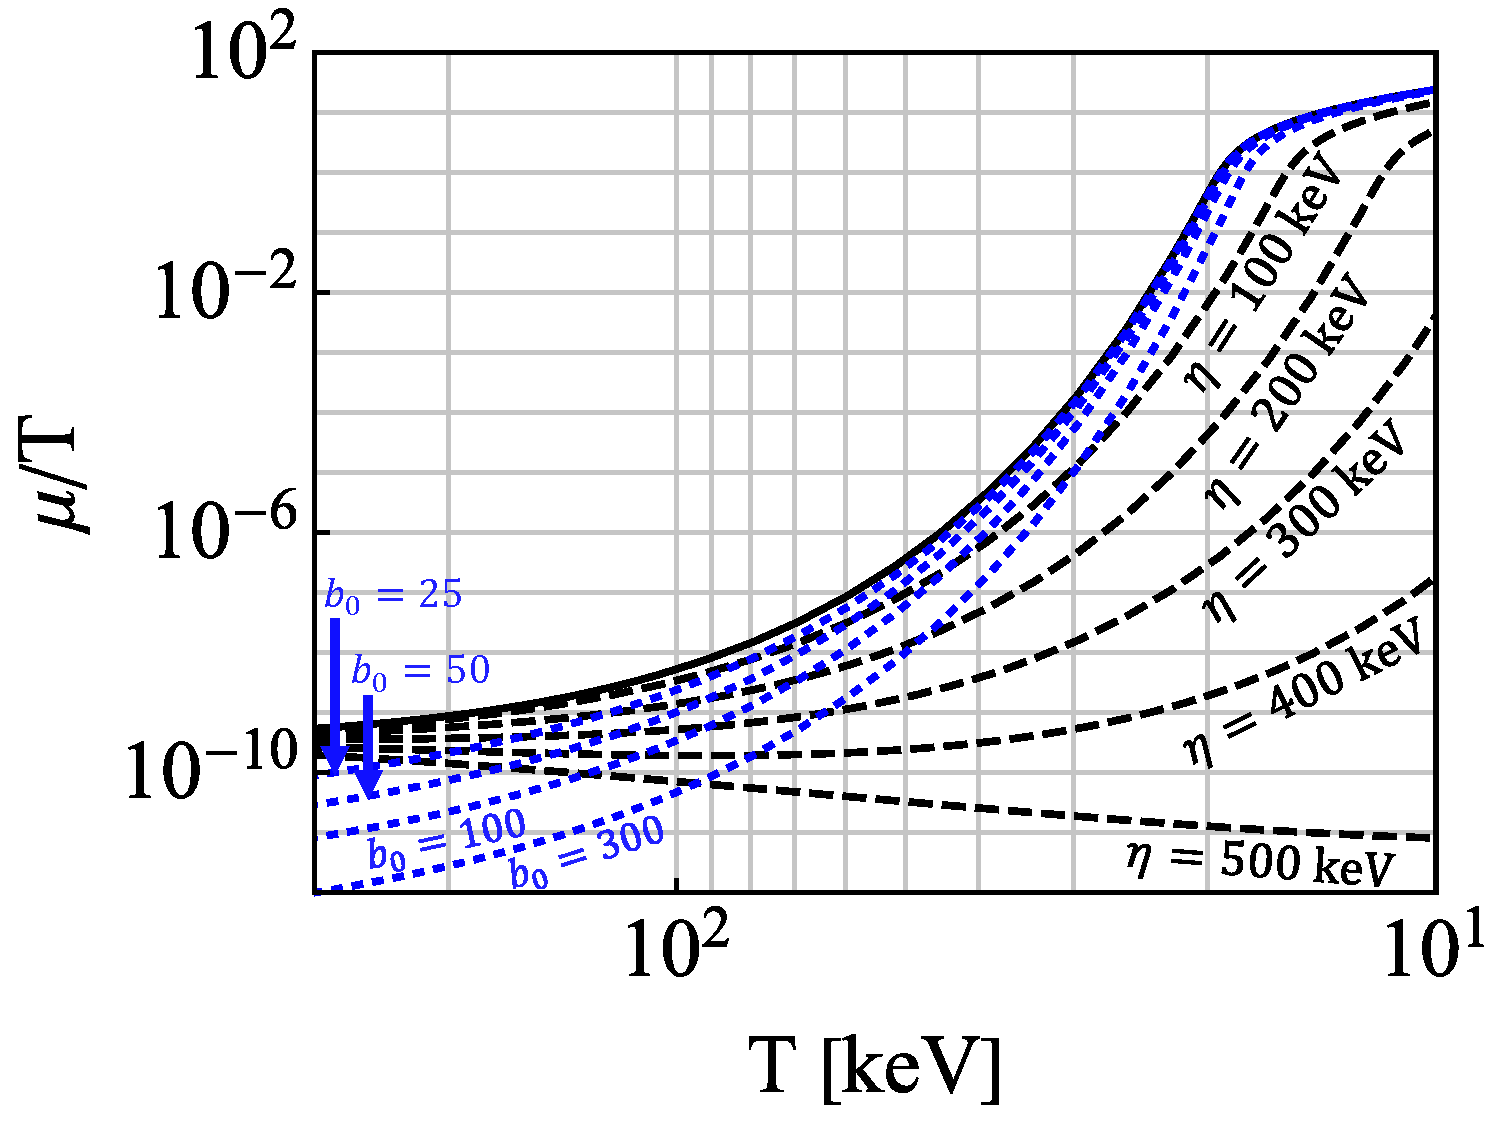
\includegraphics[clip, trim=0.0cm 0.0cm 0.0cm 0.0cm,width=0.95\linewidth]{plots/chap04cosmo/thesis_chempot_fixed.pdf}
 \caption{The chemical potential over temperature $\mu/T$ is plotted as a function of temperature with differing values of spin potential $\eta$ and magnetic scale $b_{0}$.}
 \label{fig:chemicalpotential}
\end{figure}
%%%%%%%%%%%%%%%%%%%%%%%%%%%%%%%%%%%%%%%

\req{chem} simplifies if there is no external magnetic field $b_{0}=0$ into
\begin{align}
    \label{simpchem:1}
    \sinh\frac{\mu}{T}=n_{p}\frac{\pi^{2}}{T^{3}}\left[2\cosh\frac{\eta}{T}\left(\frac{m_{e}}{T}\right)^{2}K_{2}\left(\frac{m_{e}}{T}\right)\right]^{-1}\,.
\end{align}

In \rf{fig:chemicalpotential} we plot the chemical potential $\mu/T$ in \req{chem} and \req{simpchem:1} which characterizes the importance of the charged lepton asymmetry as a function of temperature. Since the baryon (and thus charged lepton) asymmetry remains fixed, the suppression of $\mu/T$ at high temperatures indicates a large pair density which is seen explicitly in \rf{fig:densityratio}. The black line corresponds to the $b_{0}=0$ and $\eta=0$ case. 

The para-diamagnetic contribution from \req{spinorbit} does not appreciably influence $\mu/T$ until the magnetic scales involved become incredibly large well outside the observational bounds defined in \req{igmf} and \req{tbscale} as seen by the dotted blue curves of various large values $b_{0}=\{25,\ 50,\ 100,\ 300\}$. The chemical potential is also insensitive to forcing by the spin potential until $\eta$ reaches a significant fraction of the electron mass $m_{e}$ in size. The chemical potential for large values of spin potential $\eta=\{100,\ 200,\ 300,\ 400,\ 500\}\,\keV$ are also plotted as dashed black lines with $b_{0}=0$.

It is interesting to note that there are crossing points where a given chemical potential can be described as either an imbalance in spin-polarization or presence of external magnetic field. While spin potential suppresses the chemical potential at low temperatures, external magnetic fields only suppress the chemical potential at high temperatures.

The profound insensitivity of the chemical potential to these parameters justifies the use of the free particle chemical potential (black line) in the ranges of magnetic field strength considered for cosmology. Mathematically this can be understood as $\xi$ and $b_{0}$ act as small corrections in the denominator of \req{chem} if expanded in powers of these two parameters.

%%%%%%%%%%%%%%%%%%%%%%%%%%%%%%%%%%%%%%%
\section{Relativistic paramagnetism of electron-positron gas}
\label{sec:magnetization}
%%%%%%%%%%%%%%%%%%%%%%%%%%%%%%%%%%%%%%%
\noindent The total magnetic flux within a region of space can be written as the sum of external fields and the magnetization of the medium via
\begin{align}
 \label{totalmag}
 {B}_\mathrm{total} = {B} + \mathcal{M}\,.
\end{align}
For the simplest mediums without ferromagnetic or hysteresis considerations, the relationship can be parameterized by the susceptibility $\chi$ of the medium as
\begin{align}
 \label{susceptibility}
 {B}_\mathrm{total} = (1+\chi){B}\,,\qquad \mathcal{M} = \chi{B}\,,\qquad \chi\equiv\frac{\partial\mathcal{M}}{\partial{B}}\,,
\end{align}
with the possibility of both paramagnetic materials $(\chi>1)$ and diamagnetic materials $(\chi<1)$. The $e^{+}e^{-}$ plasma however does not so neatly fit in either category as given by \req{spin} and \req{spinorbit}. In general, the susceptibility of the gas will itself be a field dependant quantity.

In our analysis, the external magnetic field always appears within the context of the magnetic scale $b_{0}$, therefore we can introduce the change of variables
\begin{align}
 \frac{\partial b_{0}}{\partial{B}}=\frac{e}{T^{2}}\,.
\end{align}
The magnetization of the $e^{+}e^{-}$ plasma described by the partition function in \req{boltzmann} can then be written as
\begin{align}
 \label{defmagetization}
 \mathcal{M}\equiv\frac{T}{V}\frac{\partial}{\partial{B}}\ln{\mathcal{Z}_{e^{+}e^{-}}} = \frac{T}{V}\left(\frac{\partial b_{0}}{\partial{B}}\right)\frac{\partial}{\partial b_{0}}\ln{\mathcal{Z}_{e^{+}e^{-}}}\,,
\end{align}
Magnetization arising from other components in the cosmic gas (protons, neutrinos, etc.) could in principle also be included. Localized inhomogeneities of matter evolution are often non-trivial and generally be solved numerically using magneto-hydrodynamics (MHD)~\cite{melrose2008quantum,Vazza:2017qge,Vachaspati:2020blt} or with a suitable Boltzmann-Vlasov transport equation. An extension of our work would be to embed magnetization into transport theory~\cite{Formanek:2021blc}. In the context of MHD, primordial magnetogenesis from fluid flows in the electron-positron epoch was considered in~\cite{Gopal:2004ut,Perrone:2021srr}.

We introduce dimensionless units for magnetization ${\mathfrak M}$ by defining the critical field strength
\begin{align}
 {B}_{C}\equiv\frac{m_{e}^{2}}{e}\,,\qquad{\mathfrak M}\equiv\frac{\mathcal{M}}{{B}_{C}}\,.
\end{align}
The scale ${B}_{C}$ is where electromagnetism is expected to become subject to non-linear effects, though luckily in our regime of interest, electrodynamics should be linear. We note however that the upper bounds of IGMFs in \req{igmf} (with $b_{0}=10^{-3}$; see \req{tbscale}) brings us to within $1\%$ of that limit for the external field strength in the temperature range considered.

The total magnetization ${\mathfrak M}$ can be broken into the sum of magnetic moment parallel ${\mathfrak M}_{+}$ and magnetic moment anti-parallel ${\mathfrak M}_{-}$ contributions
\begin{align}
\label{g2mag}
{\mathfrak M}={\mathfrak M}_{+}+{\mathfrak M}_{-}\,.
\end{align}
We note that the expression for the magnetization simplifies significantly for $g\!=\!2$ which is the `natural' gyro-magnetic factor~\cite{Evans:2022fsu,Rafelski:2022bsv} for Dirac particles. For illustration, the $g\!=\!2$ magnetization from \req{defmagetization} is then
\begin{align}
 \label{g2magplus}
 {\mathfrak M}_{+}&=\frac{e^{2}}{\pi^{2}}\frac{T^{2}}{m_{e}^{2}}\xi\cosh{\frac{\mu}{T}}\left[\frac{1}{2}x_{+}K_{1}(x_{+})+\frac{b_{0}}{6}K_{0}(x_{+})\right]\,,\\
 \label{g2magminus}
 -{\mathfrak M}_{-}&=\frac{e^{2}}{\pi^{2}}\frac{T^{2}}{m_{e}^{2}}\xi^{-1}\cosh{\frac{\mu}{T}}
 \left[\left(\frac{1}{2}+\frac{b_{0}^{2}}{12x_{-}^{2}}\right)x_{-}K_{1}(x_{-})+\frac{b_{0}}{3}K_{0}(x_{-})\right]\,,\\
 x_{+}&=\frac{m_{e}}{T}\,,\qquad
 x_{-}=\sqrt{\frac{m_{e}^{2}}{T^{2}}+2b_{0}}\,.
\end{align}
As the $g$-factor of the electron is only slightly above two at $g\simeq2.00232$~\cite{Tiesinga:2021myr}, the above two expressions for ${\mathfrak M}_{+}$ and ${\mathfrak M}_{-}$ are only modified by a small amount because of anomalous magnetic moment (AMM) and would be otherwise invisible on our figures.

%%%%%%%%%%%%%%%%%%%%%%%%%%%%%%%%%%%%%%%
\subsection{Evolution of electron-positron magnetization}
\label{sec:paramagnetism}
%%%%%%%%%%%%%%%%%%%%%%%%%%%%%%%%%%%%%%%
\noindent In \rf{fig:magnet}, we plot the magnetization as given by \req{g2magplus} and \req{g2magminus} with the spin potential set to unity $\xi=1$. The lower (solid red) and upper (solid blue) bounds for cosmic magnetic scale $b_{0}$ are included. The external magnetic field strength ${B}/{B}_{C}$ is also plotted for lower (dotted red) and upper (dotted blue) bounds. Since the derivative of the partition function governing magnetization may manifest differences between Fermi-Dirac and the here used Boltzmann limit more acutely, out of abundance of caution, we indicate extrapolation outside the domain of validity of the Boltzmann limit with dashes.

%%%%%%%%%%%%%%%%%%%%%%%%%%%%%%%%%%%%%%%
\begin{figure}[ht]
 \centering
 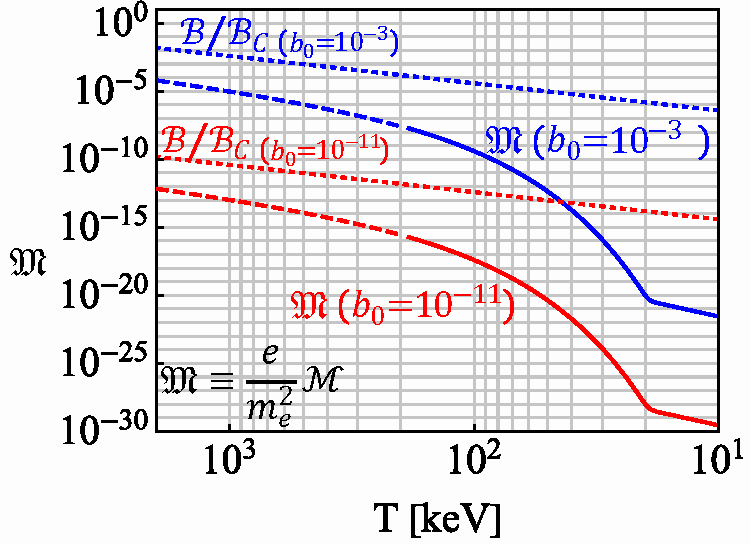
\includegraphics[width=0.95\linewidth]{plots/chap04cosmo/thesis_mag.pdf}
 \caption{The magnetization ${\mathfrak M}$, with $g\!=\!2$, of the primordial $e^{+}e^{-}$ plasma is plotted as a function of temperature. Figure made in collaboration with Cheng Tao Yang.}
 \label{fig:magnet} 
\end{figure}
%%%%%%%%%%%%%%%%%%%%%%%%%%%%%%%%%%%%%%%

We see in \rf{fig:magnet} that the $e^{+}e^{-}$ plasma is overall paramagnetic and yields a positive overall magnetization which is contrary to the traditional assumption that matter-antimatter plasma lack significant magnetic responses of their own in the bulk. With that said, the magnetization never exceeds the external field under the parameters considered which shows a lack of ferromagnetic behavior. 

The large abundance of pairs causes the smallness of the chemical potential seen in~\rf{fig:chemicalpotential} at high temperatures. As the universe expands and temperature decreases, there is a rapid decrease of the density $n_{e^{\pm}}$ of $e^{+}e^{-}$ pairs. This is the primary the cause of the rapid paramagnetic decrease seen in \rf{fig:magnet} above $T\!=\!21\keV$. At lower temperatures $T<21\keV$ there remains a small electron excess (see~\rf{fig:densityratio}) needed to neutralize proton charge. These excess electrons then govern the residual magnetization and dilutes with cosmic expansion.

An interesting feature of \rf{fig:magnet} is that the magnetization in the full temperature range increases as a function of temperature. This is contrary to Curie's law~\cite{greiner2012thermodynamics} which stipulates that paramagnetic susceptibility of a laboratory material is inversely proportional to temperature. However, Curie's law applies to systems with fixed number of particles which is not true in our situation; see \rsec{sec:perlepton}.

A further consideration is possible hysteresis as the $e^{+}e^{-}$ density drops with temperature. It is not immediately obvious the gas's magnetization should simply `degauss' so rapidly without further consequence. If the very large paramagnetic susceptibility present for $T\simeq m_{e}$ is the origin of an overall magnetization of the plasma, the conservation of magnetic flux through the comoving surface ensures that the initial residual magnetization is preserved at a lower temperature by Faraday induced kinetic flow processes however our model presented here cannot account for such effects.

Early universe conditions may also apply to some extreme stellar objects with rapid change in $n_{e^{\pm}}$ with temperatures above $T\!=\!21\keV$. Production and annihilation of $e^{+}e^{-}$ plasmas is also predicted around compact stellar objects~\cite{Ruffini:2009hg,Ruffini:2012it} potentially as a source of gamma-ray bursts.

%%%%%%%%%%%%%%%%%%%%%%%%%%%%%%%%%%%%%%%
\subsection{Dependency on g-factor}
\label{sec:gfac}
%%%%%%%%%%%%%%%%%%%%%%%%%%%%%%%%%%%%%%%

\noindent As discussed at the end of \rsec{sec:magnetization}, the AMM of $e^{+}e^{-}$ is not relevant in the present model. However out of academic interest, it is valuable to consider how magnetization is effected by changing the $g$-factor significantly.

%%%%%%%%%%%%%%%%%%%%%%%%%%%%%%%%%%%%%%%
\begin{figure}[ht]
 \centering
 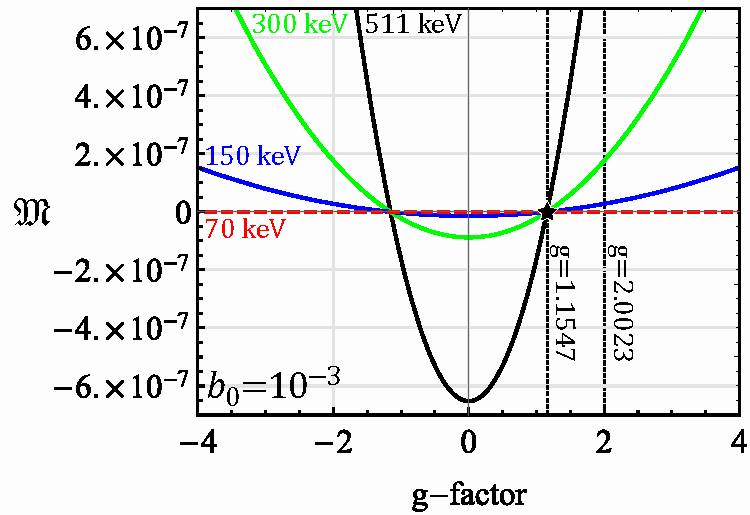
\includegraphics[width=0.95\textwidth]{plots/chap04cosmo/thesis_gfac.pdf}
 \caption{The magnetization $\mathfrak M$ as a function of $g$-factor plotted for several temperatures with magnetic scale $b_{0}=10^{-3}$ and polarization fugacity $\xi=1$.}
 \label{fig:gfac} 
\end{figure}
%%%%%%%%%%%%%%%%%%%%%%%%%%%%%%%%%%%%%%%

The influence of AMM would be more relevant for the magnetization of baryon gasses since the $g$-factor for protons $(g\approx5.6)$ and neutrons $(g\approx3.8)$ are substantially different from $g\!=\!2$. The influence of AMM on the magnetization of thermal systems with large baryon content (neutron stars, magnetars, hypothetical bose stars, etc.) is therefore also of interest~\cite{Ferrer:2019xlr,Ferrer:2023pgq}.

\req{g2magplus} and \req{g2magminus} with arbitrary $g$ reintroduced is given by
\begin{gather}
\label{arbg:1}
{\mathfrak M}=\frac{e^{2}}{\pi^{2}}\frac{T^{2}}{m_{e}^{2}}\sum_{s'}^{\pm1}\xi_{s'}\cosh{\frac{\mu}{T}}
\left[C^{1}_{s'}(x_{s'})K_{1}(x_{s'})+C^{0}_{s'}K_{0}(x_{s'})\right]\,,\\
\label{arbg:2}
C^{1}_{s'}(x_{\pm}) = \left[\frac{1}{2}-\left(\frac{1}{2}-\frac{g}{4}s'\right)\left(1+\frac{b^2_0}{12x^{2}_{s'}}\right)\right]x_{s'}\,,\qquad
C^{0}_{s'} = \left[\frac{1}{6}-\left(\frac{1}{4}-\frac{g}{8}s'\right)\right]b_0\,,
\end{gather}
where $x_{s'}$ was previously defined in \req{xfunc}.

In \rf{fig:gfac}, we plot the magnetization as a function of $g$-factor between $4>g>-4$ for temperatures $T\!=\!\{511,\ 300,\ 150,\ 70\}\keV$. We find that the magnetization is sensitive to the value of AMM revealing a transition point between paramagnetic $({\mathfrak M}>0)$ and diamagnetic gasses $({\mathfrak M}<0)$. Curiously, the transition point was numerically determined to be around $g\simeq1.1547$ in the limit $b_{0}\rightarrow0$. The exact position of this transition point however was found to be both temperature and $b_{0}$ sensitive, though it moved little in the ranges considered.

It is not surprising for there to be a transition between diamagnetism and paramagnetism given that the partition function (see \req{spin} and \req{spinorbit}) contained elements of both. With that said, the transition point presented at $g\approx1.15$ should not be taken as exact because of the approximations used to obtain the above results. 

It is likely that the exact transition point has been altered by our taking of the Boltzmann approximation and Euler-Maclaurin integration steps. It is known that the Klein-Gordon-Pauli solutions to the Landau problem in \req{cosmokgp} have periodic behavior~\cite{Steinmetz:2018ryf,Evans:2022fsu,Rafelski:2022bsv} for $|g|=k/2$ (where $k\in1,2,3\ldots$).

These integer and half-integer points represent when the two Landau towers of orbital levels match up exactly. Therefore, we propose a more natural transition between the spinless diamagnetic gas of $g=0$ and a paramagnetic gas is $g=1$. A more careful analysis is required to confirm this, but that our numerical value is close to unity is suggestive.

%%%%%%%%%%%%%%%%%%%%%%%%%%%%%%%%%%%%%%%
\subsection{Magnetization per lepton}
\label{sec:perlepton}
%%%%%%%%%%%%%%%%%%%%%%%%%%%%%%%%%%%%%%%
\noindent Despite the relatively large magnetization seen in \rf{fig:magnet}, the average contribution per lepton is only a small fraction of its overall magnetic moment indicating the magnetization is only loosely organized. Specifically, the magnetization regime we are in is described by
\begin{align}
 \label{fractionalmagnetization}
 \mathcal{M}\ll\mu_{B}\frac{N_{e^{+}}+N_{e^{-}}}{V}\,,\qquad\mu_{B}\equiv\frac{e}{2m_{e}}\,,
\end{align}
where $\mu_{B}$ is the Bohr magneton and $N=nV$ is the total particle number in the proper volume V. To better demonstrate that the plasma is only weakly magnetized, we define the average magnetic moment per lepton given by along the field ($z$-direction) axis as
\begin{align}
 \label{momentperlepton}
 \vert\vec{m}\vert_{z}\equiv\frac{\mathcal{M}}{n_{e^{-}}+n_{e^{+}}}\,,\qquad\vert\vec{m}\vert_{x}=\vert\vec{m}\vert_{y}=0\,.
\end{align}
Statistically, we expect the transverse expectation values to be zero. We emphasize here that despite $|\vec{m}|_{z}$ being nonzero, this doesn't indicate a nonzero spin angular momentum as our plasma is nearly matter-antimatter symmetric. The quantity defined in \req{momentperlepton} gives us an insight into the microscopic response of the plasma.

%%%%%%%%%%%%%%%%%%%%%%%%%%%%%%%%%%%%%%%
\begin{figure}[ht]
 \centering
 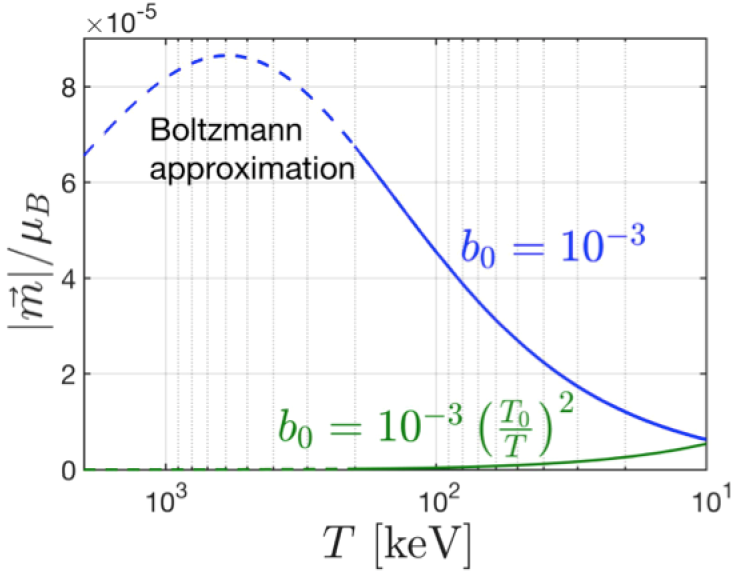
\includegraphics[clip, trim=0.0cm 0.0cm 0.0cm 0.0cm,width=0.95\textwidth]{plots/chap04cosmo/thesis_perlepton.png}
 \caption{The magnetic moment per lepton $\vert\vec{m}\vert_{z}$ along the field axis as a function of temperature. Figure made in collaboration with Cheng Tao Yang.}
 \label{fig:momentperlepton}
\end{figure}
%%%%%%%%%%%%%%%%%%%%%%%%%%%%%%%%%%%%%%%

The average magnetic moment $\vert\vec{m}\vert_{z}$ defined in \req{momentperlepton} is plotted in \rf{fig:momentperlepton} which displays how essential the external field is on the `per lepton' magnetization. The $b_{0}=10^{-3}$ case (blue curve) is plotted in the Boltzmann approximation. The dashed lines indicate where this approximation is only qualitatively correct. For illustration, a constant magnetic field case (solid green line) with a comoving reference value chosen at temperature $T_{0}=10\keV$ is also plotted.

If the field strength is held constant, then the average magnetic moment per lepton is suppressed at higher temperatures as expected for magnetization satisfying Curie's law. The difference in \rf{fig:momentperlepton} between the non-constant (blue solid curve) case and the constant field (solid green curve) case demonstrates the importance of the conservation of primordial magnetic flux in the plasma, required by \req{bscale}. While not shown, if \rf{fig:momentperlepton} was extended to lower temperatures, the magnetization per lepton of the constant field case would be greater than the non-constant case which agrees with our intuition that magnetization is easier to achieve at lower temperatures. This feature again highlights the importance of flux conservation in the system and the uniqueness of the primordial cosmic environment.

%%%%%%%%%%%%%%%%%%%%%%%%%%%%%%%%%%%%%%%
\section{Polarization potential and ferromagnetism}
\label{sec:ferro}
%%%%%%%%%%%%%%%%%%%%%%%%%%%%%%%%%%%%%%%
\noindent Up to this point, we have neglected the impact that a nonzero spin potential $\eta\neq0$ (and thus $\xi\neq1$) would have on the primordial $e^{+}e^{-}$ plasma magnetization. In the limit that $(m_{e}/T)^2\gg b_0$ the magnetization given in \req{arbg:1} and \req{arbg:2} is entirely controlled by the spin fugacity $\xi$ asymmetry generated by the spin potential $\eta$ yielding up to first order $\mathcal{O}(b_{0})$ in magnetic scale
\begin{multline}
 \label{ferro}
 \lim_{m_{e}^{2}/T^{2}\gg b_0}{\mathfrak M}=\frac{g}{2}\frac{e^{2}}{\pi^{2}}\frac{T^{2}}{m_{e}^{2}}\sinh{\frac{\eta}{T}}\cosh{\frac{\mu}{T}}\left[\frac{m_{e}}{T}K_{1}\left(\frac{m_{e}}{T}\right)\right]\\
 +b_{0}\left(g^{2}-\frac{4}{3}\right)\frac{e^{2}}{8\pi^{2}}\frac{T^{2}}{m_{e}^{2}}\cosh{\frac{\eta}{T}}\cosh{\frac{\mu}{T}}K_{0}\left(\frac{m_{e}}{T}\right)
 +\mathcal{O}\left(b_{0}^{2}\right)
\end{multline}

Given \req{ferro}, we can understand the spin potential as a kind of `ferromagnetic' influence on the primordial gas which allows for magnetization even in the absence of external magnetic fields. This interpretation is reinforced by the fact the leading coefficient is $g/2$.

We suggest that a variety of physics could produce a small nonzero $\eta$ within a domain of the gas. Such asymmetries could also originate statistically as while the expectation value of free gas polarization is zero, the variance is likely not.

As $\sinh{\eta/T}$ is an odd function, the sign of $\eta$ also controls the alignment of the magnetization. In the high temperature limit \req{ferro} with strictly $b_{0}=0$ assumes a form of to lowest order for brevity
\begin{align}
 \label{hiTferro}
 \lim_{m_{e}/T\rightarrow0}{\mathfrak M}\vert_{b_{0}=0}=\frac{g}{2}\frac{e^{2}}{\pi^{2}}\frac{T^{2}}{m_{e}^{2}}\frac{\eta}{T}\,,
\end{align}

While the limit in \req{hiTferro} was calculated in only the Boltzmann limit, it is noteworthy that the high temperature (and $m\rightarrow0$) limit of Fermi-Dirac distributions only differs from the Boltzmann result by a proportionality factor. 

The natural scale of the $e^{+}e^{-}$ magnetization with only a small spin fugacity ($\eta<1\eV$) fits easily within the bounds of the predicted magnetization during this era if the IGMF measured today was of primordial origin. The reason for this is that the magnetization seen in \req{g2magplus}, \req{g2magminus} and \req{ferro} are scaled by $\alpha{B}_{C}$ where $\alpha$ is the fine structure constant.

%%%%%%%%%%%%%%%%%%%%%%%%%%%%%%%%%%%%%%%
\subsection{Hypothesis of ferromagnetic self-magnetization}
\label{sec:self}
%%%%%%%%%%%%%%%%%%%%%%%%%%%%%%%%%%%%%%%
\noindent One exploratory model we propose is to fix the spin polarization asymmetry, described in \req{spotential}, to generate a homogeneous magnetic field which dissipates as the universe cools down. In this model, there is no external primordial magnetic field $({B}_\mathrm{PMF}=0)$ generated by some unrelated physics, but rather the $e^{+}e^{-}$ plasma itself is responsible for the field by virtue of spin polarization.

%%%%%%%%%%%%%%%%%%%%%%%%%%%%%%%%%%%%%%%
\begin{figure}[ht]
 \centering
 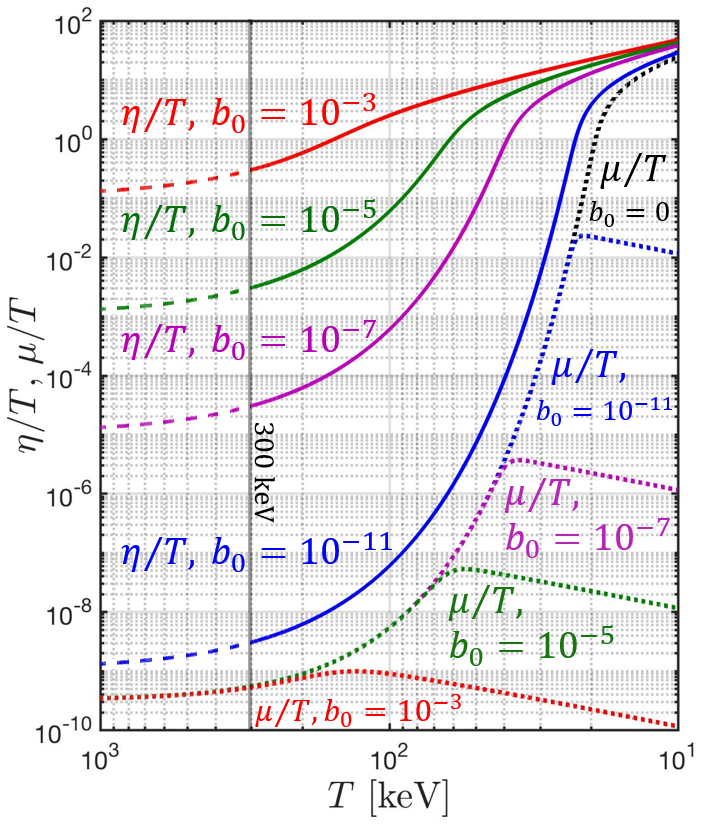
\includegraphics[width=0.5\textwidth]{plots/chap04cosmo/Spinchemical_03.png}
 \caption{The spin potential $\eta$ and chemical potential $\mu$ are plotted under the assumption of self-magnetization through a nonzero spin polarization in bulk of the plasma. Figure made in collaboration with Cheng Tao Yang.}
 \label{fig:self} 
\end{figure}
%%%%%%%%%%%%%%%%%%%%%%%%%%%%%%%%%%%%%%%

This would obey the following assumption of
\begin{align}
 \label{selfmag}
 {\mathfrak M}(b_{0})=\frac{\mathcal{M}(b_0)}{{B}_{C}}\longleftrightarrow\frac{B}{{B}_{C}}=b_{0}\frac{T^{2}}{m_{e}^{2}}\,,
\end{align}
which sets the total magnetization as a function of itself. The spin polarization described by $\eta\rightarrow\eta(b_{0},T)$ then becomes a fixed function of the temperature and magnetic scale. The underlying assumption would be the preservation of the homogeneous field would be maintained by scattering within the gas (as it is still in thermal equilibrium) modulating the polarization to conserve total magnetic flux.

The result of the self-magnetization assumption in \req{selfmag} for the potentials is plotted in \rf{fig:self}. The solid lines indicate the curves for $\eta/T$ for differing values of $b_{0}=\{10^{-11},\ 10^{-7},\ 10^{-5},\ 10^{-3}\}$ which become dashed above $T\!=\!300\keV$ to indicate that the Boltzmann approximation is no longer appropriate though the general trend should remain unchanged.

%%%%%%%%%%%%%%%%%%%%%%%%%%%%%%%%%%%%%%%
\begin{figure}[ht]
 \centering
 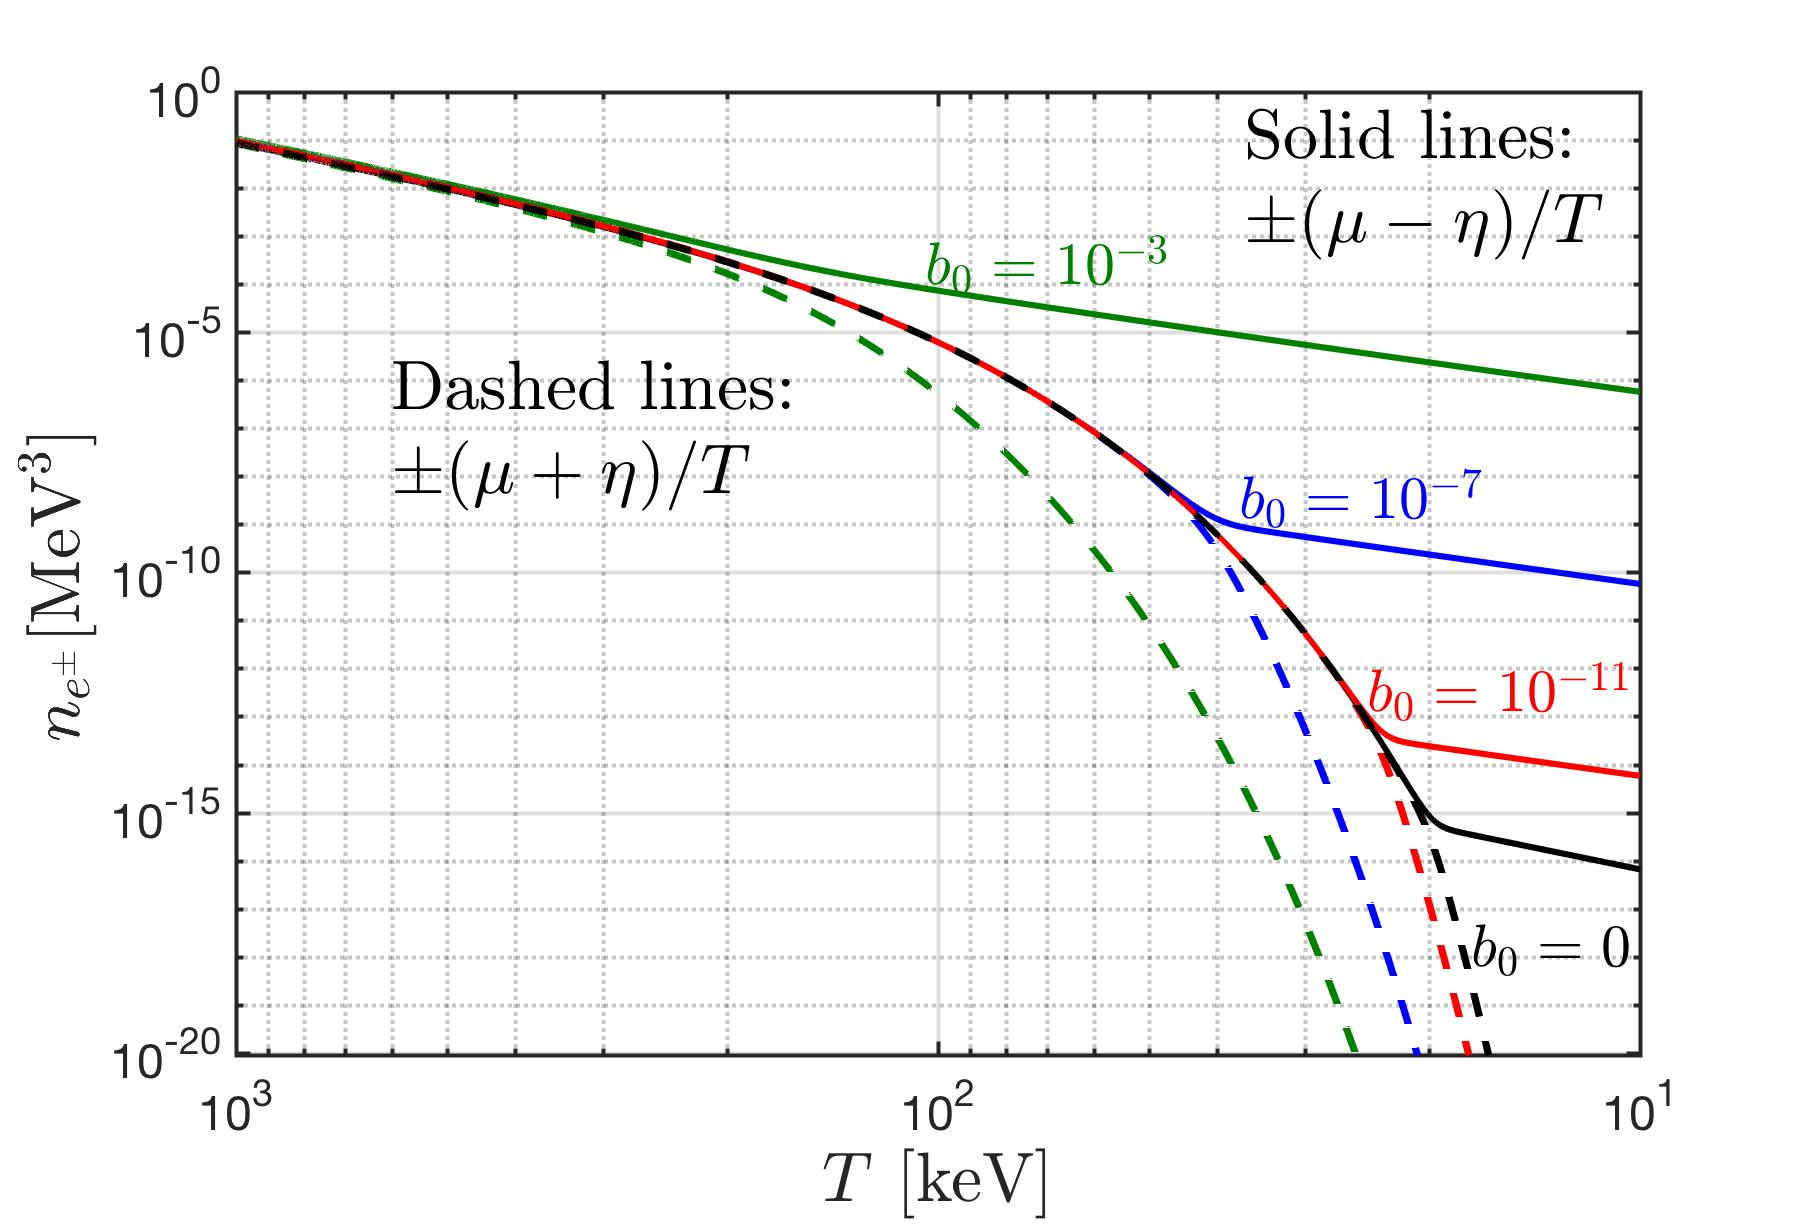
\includegraphics[width=0.95\textwidth]{plots/chap04cosmo/ElectronDensity_SpinChemicalPotential004.jpg}
 \caption{The number density $n_{e^{\pm}}$ of polarized electrons and positrons under the self-magnetization model for differing values of $b_{0}$. Figure courtesy of Cheng Tao Yang.}
 \label{fig:polarswap} 
\end{figure}
%%%%%%%%%%%%%%%%%%%%%%%%%%%%%%%%%%%%%%%

The dotted lines are the curves for the chemical potential $\mu/T$. At high temperatures we see that a relatively small $\eta/T$ is needed to produce magnetization owing to the large densities present. \rf{fig:self} also shows that the chemical potential does not deviate from the free particle case until the spin polarization becomes sufficiently high which indicates that this form of self-magnetization would require the annihilation of positrons to be incomplete even at lower temperatures.

This is seen explicitly in~\rf{fig:polarswap} where we plot the numerical density of particles as a function of temperature for spin aligned $(+\eta)$ and spin anti-aligned $(-\eta)$ species for both positrons $(-\mu)$ and electrons $(+\mu)$. Various self-magnetization strengths are also plotted to match those seen in~\rf{fig:self}. The nature of $T_{\rm split}$ changes under this model since antimatter and polarization states can be extinguished separately. Positrons persist where there is insufficient electron density to maintain the magnetic flux. Polarization asymmetry therefore appears physical only in the domain where there is a large number of matter-antimatter pairs.

%%%%%%%%%%%%%%%%%%%%%%%%%%%%%%%%%%%%%%%
\subsection{Matter inhomogeneities in the cosmic plasma}
\label{sec:inhomogeneous}
%%%%%%%%%%%%%%%%%%%%%%%%%%%%%%%%%%%%%%%
\noindent In general, an additional physical constraint is required to fully determine $\mu$ and $\eta$ simultaneously as both potentials have mutual dependency (see \rsec{sec:ferro}). We note that spin polarizations are not required to be in balanced within a single species to preserve angular momentum.

The CMB~\cite{Planck:2018vyg} indicates that the early universe was home to domains of slightly higher and lower baryon densities which resulted in the presence of galactic super-clusters, cosmic filaments, and great voids seen today. However, the CMB, as measured today, is blind to the localized inhomogeneities required for gravity to begin galaxy and supermassive black hole formation.

Such acute inhomogeneities distributed like a dust~\cite{Grayson:2023flr} in the plasma would make the proton density sharply and spatially dependant $n_{p}\rightarrow n_{p}(x)$ which would directly affect the potentials $\mu(x)$ and $\eta(x)$ and thus the density of electrons and positrons locally. This suggests that $e^{+}e^{-}$ may play a role in the initial seeding of gravitational collapse. If the plasma were home to such localized magnetic domains, the nonzero local angular momentum within these domains would provide a natural mechanism for the formation of rotating galaxies today.

Recent measurements by the James Webb Space Telescope (JWST)~\cite{Yan:2022sxd,adams2023discovery,arrabal2023spectroscopic} indicate that galaxy formation began surprisingly early at large redshift values of $z\gtrsim10$ within the first 500 million years of the universe requiring gravitational collapse to begin in a hotter environment than expected. The observation of supermassive black holes already present~\cite{CEERSTeam:2023qgy} in this same high redshift period (with millions of solar masses) indicates the need for local high density regions in the early universe whose generation is not yet explained and likely need to exist long before the recombination epoch.

%%%%%%%%%%%%%%%%%%%%%%%%

\bibliographystyle{spphys}
\bibliography{bibs/birrell-refs,bibs/steinmetz-refs,bibs/yang-refs}
%%%%%%%%%%%%%%%%%%%%%%%%
\end{document}
